%\documentclass[journal,10pt,onecolumn]{IEEEtran}
\documentclass[12pt,draftcls,onecolumn]{IEEEtran}

\ifCLASSINFOpdf
\else
   \usepackage[dvips]{graphicx}
\fi
\usepackage{url}
\hyphenation{op-tical net-works semi-conduc-tor}
\usepackage{graphicx}
\usepackage{amsmath}
\usepackage{comment}
\usepackage[utf8]{inputenc}
\usepackage[english]{babel}
\usepackage{color}
\usepackage{framed}
\usepackage{cite}
\usepackage{amssymb,amsfonts}
%\usepackage{algorithmic}
%\usepackage{algorithm}
%\usepackage{algpseudocode}
%\usepackage{graphicx}
\usepackage{textcomp}
%\usepackage{xcolor}
% *** CITATION PACKAGES ***
\usepackage{cite}
\renewcommand*{\citepunct}{, } % Was {], [}
\renewcommand*{\citedash}{--}  % Was {]--[}

%\usepackage{cite}
\usepackage{bbold}
\usepackage{ifpdf}
\usepackage{times}
\usepackage{layout}
\usepackage{float}
\usepackage{afterpage}
%\usepackage{amsmath}
\usepackage{amstext}
\usepackage{amssymb,bm}
\usepackage{latexsym}
\usepackage{color}
\usepackage{flexisym}
%\usepackage{dblfloatfix}    % To enable figures at the bottom of page
\usepackage{kantlipsum}
%\usepackage{subcaption}
%\usepackage{graphicx}
%\usepackage{amsmath}
\usepackage{amsthm}
\usepackage{upgreek}
%\usepackage{graphicx}
%\usepackage{caption}
%\usepackage{subcaption}

% *** SUBFIGURE PACKAGES ***
\usepackage[caption=false,font=footnotesize]{subfig}

\usepackage{booktabs}
\usepackage{multicol}
%\usepackage{lipsum}% dummy text
\let\labelindent\relax
\usepackage{enumitem}
%\usepackage[]{algorithm2e}
\input{symbols.tex}
\DeclareMathOperator*{\argmin}{arg\,min}
%\documentclass{article}
\makeatletter
\newcommand*{\rom}[1]{\expandafter\@slowromancap\romannumeral #1@}
\makeatother
\def\at{\Tilde{a}}
\def\bt{\Tilde{b}}
\newcommand{\stcomp}[1]{{#1}^\complement}
\newcommand{\ms}[1]{\textcolor{cyan}{#1}}
\newcommand{\Ae}[1]{\textcolor{red}{#1}}
\newcommand{\Fr}[1]{\textcolor{blue}{#1}}
\begin{document}

%\title{ORKA: Accelerated Kaczmarz Algorithms for Signal Recovery from One-Bit Samples}
%\title{One-Bit Sensing With Time-Varying Sampling Thresholds:\\
%\title{One-Bit Sensing via Sample Abundance:\\
%Theoretical Guarantees and Accelerated Kaczmarz Algorithms}
%\title{The Power of Plenty: Theoretical Guarantees and Accelerated Kaczmarz Algorithms for Efficient One-Bit Sensing}
\title{Harnessing the Power of Sample Abundance: Theoretical Guarantees and Algorithms for Accelerated One-Bit Sensing}
\author{Arian Eamaz, \IEEEmembership{Student Member, IEEE}, Farhang Yeganegi, Deanna Needell, \IEEEmembership{Member, IEEE}, and \\ Mojtaba Soltanalian, \IEEEmembership{Senior Member, IEEE}
\thanks{This work relates in part to Department of Navy Award N00014-22-1-2666 issued by the Office of Naval Research. Any opinions, findings, conclusions, or recommendations expressed in
this material are those of the authors and do not necessarily reflect the views of the
Office of Naval Research. A conference precursor to this work was presented at the 2023 IEEE International Symposium on Information Theory (ISIT). The first two authors contributed equally to this work.}
\thanks{A. Eamaz, F. Yeganegi, and M. Soltanalian are with the Department of Electrical and Computer Engineering, University of Illinois Chicago, Chicago, IL 60607, USA (\emph{Corresponding author: Arian Eamaz}).
}
\thanks{D. Needell is with the Department of Mathematics, University of California Los Angeles, Los
Angeles, CA 90095, USA.}
}

\markboth{Submitted to the IEEE TRANSACTIONS ON INFORMATION THEORY, 2023
}
{Shell \MakeLowercase{\textit{et al.}}: Bare Demo of IEEEtran.cls for IEEE Journals}
\maketitle

\begin{abstract}
One-bit quantization with time-varying sampling thresholds (also known as random dithering)
has recently found significant utilization potential in statistical signal processing applications due to its relatively low
power consumption and low implementation cost. In addition
to such advantages, an attractive feature of one-bit analog-to-digital converters (ADCs) is their superior sampling rates as compared to their conventional multi-bit counterparts. This characteristic endows one-bit signal processing frameworks with what one may refer to as \emph{sample abundance}.  We show that sample abundance plays a pivotal role in many signal recovery and optimization problems that are formulated as (possibly non-convex) quadratic programs with linear feasibility constraints. Of particular interest to our work are low-rank matrix recovery and compressed sensing applications that take advantage of one-bit quantization. We demonstrate that the sample abundance paradigm allows for the transformation of such problems to merely linear feasibility problems by forming large-scale overdetermined linear systems---thus removing the need for handling costly optimization constraints and objectives. To make the proposed computational cost savings achievable, we offer enhanced randomized Kaczmarz algorithms to solve these highly overdetermined feasibility problems and provide theoretical guarantees in terms of their convergence, sample size requirements, and overall performance. Several numerical results are presented to illustrate the effectiveness of the proposed
methodologies.  
\end{abstract}


\begin{IEEEkeywords}
Convex-relaxed problems, compressed sensing, low-rank matrix sensing, one-bit quantization, one-bit ADCs, randomized Kaczmarz algorithm, statistical signal processing, time-varying sampling thresholds.
\end{IEEEkeywords}


\IEEEpeerreviewmaketitle



\section{Introduction}
%
\IEEEPARstart{W}{e} consider an optimization problem of the form:
\begin{equation}
\label{eq:1nnnn}
\begin{aligned}
\underset{\mbX \in \Omega_{c}}{\textrm{minimize}}\quad f(\mbX)\quad
\text{subject to} \quad &\mathcal{A}\left(\mbX\right)=\mathbf{y},
\end{aligned}
\end{equation}\normalsize
where $f(.)$ is a cost function, $\Omega_{c}$ is a feasible set, $\mbX\in \mathbb{C}^{n_{1}\times n_{2}}$ is the matrix of unknowns, $\mathbf{y}\in \mathbb{R}^{n}$ is the measurement vector, and $\mathcal{A}$ is a linear transformation mapping $\mathbb{C}^{n_{1}\times n_{2}}$ into $\mathbb{R}^{n}$. This problem emerges in a wide variety of applications, particularly as the relaxed variant of some well-known NP-hard problems. Although many problems can be expressed in
the form in (\ref{eq:1nnnn}), the applications we will focus on in this paper
include some specific problems of interest which can take advantage of low-resolution (and particularly one-bit) sampling and processing:
\begin{itemize}
\item The task of \emph{recovering a low-rank matrix from its linear measurements} plays a central role in computational science. The problem occurs in many areas of applied mathematics, such as signal processing \cite{candes2015phase,cai2010singular,davenport20141,davenport2016overview,candes2011tight,chen2013low,li2019survey}, machine learning \cite{haeffele2014structured,nie2012low,blei2012probabilistic,obozinski2010joint,pontile2007convex,argyriou2006multi}, and computer vision\cite{tomasi1992shape}. In this scenario, the cost function of (\ref{eq:1nnnn}), $f(.)$, is typically the nuclear norm or the Frobenius norm, and the constraint set $\Omega_{c}$ would be an amplitude restriction on the elements of matrix $\mbX$; see \cite{recht2011null,cai2010singular}.
    \item \emph{Compressed sensing} (CS) offers a framework for the simultaneous sensing and compression
of finite-dimensional vectors by relying on linear dimensionality reduction. Through a CS formulation, sparse signals may be recovered from highly incomplete measurements \cite{candes2006robust,candes2006compressive,candes2008introduction}. The problem (1) can be adopted in the CS context when $f\left(\mbX\right)=\left\|\operatorname{vec}\left(\mbX\right)\right\|_{1}$.
\end{itemize}
%Phase retrieval has received a great deal of interest as it aims to recover an unknown signal solely from phaseless
%measurements that depend on the signal through a linear
%observation, commanding numerous applications in applied physics and statistical signal processing communities over the past decades \cite{eamaz2022phase,millane,kim,Fienup93, Krist95, Sarnik,GS1,GS2,fienup1,fienup2,fienup3,candes2013phaselift, candes2014solving}. To have a convex formulation, the phase retrieval has been relaxed into semi-definite programs where the problem boils down to a trace minimization while considering the positive semi-definite constraint \cite{eamaz2022phase,candes2015phase}.
This paper will primarily concentrate on relaxation problems in which the objective function $f(\cdot)$ is relaxed to address the NP-hard cost caused due to the associated  feasibility constraints. Such relaxation techniques prove significantly helpful in various applications, such as nuclear norm minimization for low-rank matrix recovery and $\ell_1$ minimization for compressed sensing problems.

Sampling the signals of interest at high data rates with high-resolution ADCs would dramatically increase the overall manufacturing cost and power consumption of such ADCs. In multi-bit sampling scenarios, a very large number of quantization levels is necessary in order to represent the original continuous signal in with high accuracy, which in turn leads to a considerable reduction in sampling rate \cite{boufounos2015quantization,eamaz2021modified}. This attribute of multi-bit sampling is the key reason for the general emergence of underdetermined systems $n_{1}n_{2}\geq n$ in (\ref{eq:1nnnn}) \cite{candes2013phaselift,candes2015phase,eamaz2022phase}. An alternative solution to such challenges is to deploy \emph{one-bit quantization} which is an extreme sampling scenario, where the signals are merely compared with given threshold levels at the ADCs, producing sign data ($\pm1$). This enables signal processing equipments to sample at a very high rate, with a considerably lower cost and energy consumption, compared to their counterparts which employ multi-bit ADCs \cite{mezghani2018blind,eamaz2021modified,sedighi2020one,sedighi2021performance}. Several applications abound of one-bit ADCs, such as multiple-input multiple-output wireless communications \cite{kong2018multipair,mezghani2018blind,maly2022new}, channel estimation \cite{li2017channel,choi2016near}, and array signal processing \cite{liu2017one}. Extensive research on one-bit Sigma-Delta quantization explores the impact of adaptive threshold selection on achieving rapidly decaying reconstruction errors with respect to the number of measurements or the oversampling rate, depending on the scenario. For more detailed insights, readers can refer to relevant works such as \cite{gunturk2003one,deift2011optimal,benedetto2006sigma}. Various methods for one-bit quantization, including our own, offer distinct trade-offs between computational and implementation complexity and reconstruction accuracy. Take the Sigma-Delta approach as an example, which necessitates memory elements to store state-variables associated with thresholds. This sequential quantization of incoming measurements demands significant memory and computational power, causing delays in acquiring measurements while the thresholds are being updated. Therefore, sensors used to collect measurements must possess substantial computational capabilities to accommodate such requirements \cite{knudson2016one,boufounos2015quantization}. 

The classical one-bit sampling problem involves reconstructing a signal by comparing it with a fixed threshold, often set at zero. This method has limitations in accurately estimating signal parameters, especially when the input signal $\mathbf{x}$ is converted into one-bit data since the power information is lost. This occurs because the signs of $\mathbf{x}$ and $\eta\mathbf{x}$ are the same for $\eta>0$. The effectiveness of incorporating random thresholds (dithers) within the framework of one-bit quantization has been extensively established in various contexts \cite{dabeer2006signal,rousseau2003nonlinear}.
Extensive research has been dedicated to investigating the impact of thresholding (dithering) on the quantization process and its effect on quantization error \cite{schuchman1964dither, vanderkooy1987dither,  wagdy1989validity,gray1993dithered,   carbone1997quantitative, ali202012}. In the evaluation of quantizing systems, particularly in digital signal processing applications, the mean squared error (MSE) serves as a relevant parameter for assessing performance. Dithering provides the flexibility to control system performance by enabling a trade-off between accuracy and resolution. An intriguing property of dithering is its ability to reduce the overall average quantization error \cite{carbone1997quantitative}.

Various dithering schemes have been studied, including uniform dither, discrete dither, and Gaussian dither. Research findings suggest that a carefully chosen dither signal can significantly improve the resolution and performance of digital instrumentation. While discrete dithering has been examined, it generally does not perform as effectively as uniform or Gaussian dithering in terms of reducing quantization error \cite{carbone1997quantitative}.
Uniformly distributed dither sequences have been selected due to their effectiveness in minimizing the average quantization error under appropriate conditions \cite{schuchman1964dither}. Gaussian distributed dither signals, on the other hand, are favored for their ability to provide good resolution \cite{carbone1994effect, wagdy1989effect}. Furthermore, studies have shown that while Uniform dithering theoretically offers infinite resolution, its performance can rapidly deteriorate when uncertainties in dither amplitude are present. In contrast, Gaussian dithering has proven to be more robust in practical scenarios, exhibiting fewer sensitivity issues \cite{wagdy1989effect, xi2020gridless}. After a thorough analysis in \cite{carbone1997quantitative}, it becomes evident that when considering both resolution and accuracy in quantizers, the choice between Gaussian and uniformly distributed dither signals has minimal impact on the performance of the quantizing scheme.
%It is important to acknowledge that while discrete dithering may not match the performance of uniform or Gaussian dithering, it offers notable advantages in terms of practical implementation.

The implementation of a dithered generator, specifically for generating Gaussian dithering in quantization systems within an ADC system, was described in \cite{robinson2019analog}. According to their work, the dither generator produces Gaussian dithering by generating a random analog noise signal. One method of achieving this is by utilizing a low-cost thermal noise diode, which introduces analog Gaussian dither. The intrinsic quantum mechanical properties of electron-hole pairing in such devices generate a truly random noise signal. In some cases, the power levels of the noise generated by certain dither generators may be relatively small. Therefore, optional processing circuitry can be employed alongside the dither generator, which may include components such as gain control circuitry for the analog noise signal, low-cost operational amplifiers, or similar elements, as required. Additionally, the implementation of multiple random dithering was demonstrated in \cite{ali2020background} for a 12-bit, 18-GS/s ADC. 

Recent works, such as \cite{qian2017admm,gianelli2016one,wang2017angular,xi2020gridless,xu2020quantized}, have proposed using time-varying thresholds to improve the estimation of signal characteristics. For instance, \cite{eamaz2021modified} considered Gaussian dithering for recovering covariance from one-bit measurements, while \cite{eamaz2023covariance} extended this method for better estimation of signal autocorrelation through the "modified arcsine law." In non-stationary scenarios, the authors in \cite{eamaz2022covariance} utilized time-varying sampling thresholds with the modified arcsine law. In \cite{dirksen2022covariance}, the authors provide a comprehensive investigation of estimating the covariance matrix from one-bit measurements using Uniform dithering. Dithered One-bit quantization has also been applied to various problems, such as sparse parameter estimation \cite{gianelli2016one,dabeer2006signal,thrampoulidis2020generalized}, phase retrieval \cite{eamaz2022phase}, and sampling theory \cite{eamaz2022uno} as discussed in contemporary literature. The study presented in \cite{eamaz2022covariance} demonstrates that one-bit signal parameter estimation with time-varying thresholds yields notably superior results compared to using constant thresholds. Similarly, constant thresholds, just like zero thresholds, have the potential to overlook certain signal information. 
While Uniform dithering has been extensively studied and proven to offer theoretical guarantees and good performance for bounded measurements, recent studies \cite{xi2020gridless,eamaz2023covariance} have shown that Gaussian dithering outperforms Uniform dithering in signal reconstruction. Specifically, in the context of Cram\'er-Rao bound (CRB) analysis, Gaussian dithering exhibits better performance for input signals with bell-shaped distributions.
%The various methods for one-bit quantization, including our own approach, offer different trade-offs between computational and implementation complexity and the accuracy of reconstruction.

Randomized iterative algorithms have become a widely employed technique for dimension reduction, encompassing various iterative methods for solving linear systems and their variations, as well as extensions to non-linear optimization problems \cite{martinsson2020randomized}. These algorithms include well-known methods such as randomized Kaczmarz algorithm (RKA) \cite{strohmer2009randomized,dai2013randomized}, coordinate descent \cite{leventhal2010randomized, ma2015convergence}, and variants of the Newton method in convex optimization \cite{yuan2022sketched}, among others.
\emph{In this approach, instead of utilizing all available information at each iteration, a sketched subset of the information is used, selected through a sketching process.} By multiplying the data with a random matrix, randomized sketching effectively reduces the size of the problem while preserving its essential characteristics.
Common examples of sketching matrices include Gaussian matrices with independent entries and other matrices that satisfy the Johnson-Lindenstrauss property. Another example is block-identity matrices, which effectively subsample the data matrix.
The Kaczmarz method \cite{kaczmarz1937angenaherte} is an iterative projection algorithm for solving linear systems of equations and inequalities. It is usually applied to highly overdetermined systems because of its simplicity.
Each iteration projects onto the solution space corresponding to one row in the linear system, in a sequential regimen. The method has been applied to various applications in image reconstruction, digital signal processing, and
computer tomography \cite{feichtinger1995kaczmarz,sezan1987applications,eamaz2022phase}. Many variants of this iterative method and their convergence rates have been proposed and studied in recent decades for both consistent and inconsistent systems including the randomized Kaczmarz algorithm, the randomized block Kaczmarz algorithm and most recently, the sampling Kaczmarz-Motzkin method \cite{strohmer2009randomized,leventhal2010randomized,needell2014paved,briskman2015block,de2017sampling}.

\subsection{Prior Art}
Our work aligns seamlessly with the recent advancements in the exploration of coarse quantization for parameter estimation from random measurements. The emergence of one-bit compressed sensing (one-bit CS) has led to a plethora of papers that have greatly enhanced our understanding of employing dithering for one-bit signal reconstruction.

The domain of one-bit low-rank matrix sensing has garnered considerable interest, yet it remains relatively unexplored. Several noteworthy papers, such as \cite{foucart2019recovering, foucart2019one}, have shed light on this intriguing subject. In \cite{foucart2019recovering}, the authors delve into the theoretical guarantees of one-bit sensing from low-rank matrices, employing two distinct algorithms: one based on hard singular value thresholding and the other utilizing semidefinite programming.
The initial investigation in this study considers a scenario \emph{without} thresholds and subsequently progresses to the Gaussian sampling matrix and Gaussian dithering scenario, where both adaptive and non-adaptive thresholds are employed. However, the recovery algorithms and theoretical guarantees presented in this study require the availability of side information regarding the signal of interest, specifically an upper bound on the Frobenius norm of input signal. This requirement contradicts the essence of employing dithering in one-bit sensing, as the literature suggests that the primary advantage of dithering lies in the ability to recover the signal magnitude without additional information. In the notable work of \cite{foucart2019one}, the authors explore one-bit sensing for both low-rank and bisparse matrices. Notably, they achieve a significant milestone by deriving tailored theoretical guarantees for these types of matrices, providing a novel contribution to the field. Additionally, they investigate the impact of coarse quantization in thresholdless scenarios, focusing on recovering only the signal direction rather than its exact magnitude. It is worth mentioning that both of these influential papers exclusively focus on scenarios involving Gaussian sampling matrices.

One-bit CS was first introduced in \cite{boufounos20081}. Later, in \cite{jacques2013robust}, this method was extensively investigated, and they presented a lower bound on the reconstruction error, alongside proposing heuristic algorithms for recovering the underlying signals. Extensive research has been dedicated to the problem of one-bit CS \emph{without} dithering, resulting in numerous proposed approaches for its solution. Notably, the binary iterative hard thresholding (BIHT) and its normalized version, normalized BIHT (NBIHT), have emerged as prominent methods in this field \cite{boufounos20081,boufounos2015quantization,bahmani2013robust,plan2013one,jacques2013quantized,jacques2013robust,friedlander2021nbiht,matsumoto2022binary}. %In some earlier works, dithering was ignored and the signal norm was constrained to be $1$, leading to the derivation of various theoretical guarantees for reconstruction algorithms
Support recovery in one-bit CS has been extensively studied in the literature, resulting in a wealth of research that has yielded improved bounds for performance guarantees \cite{haupt2011robust,acharya2017improved,flodin2019superset}.
In some earlier works, the ditherless setup was taken into account with a further assumption on the norm of the signal, $\|\mbx\|_{2}=1$, leading to the derivation of various theoretical guarantees for reconstruction algorithms \cite{jacques2013robust,ai2014one,shi2016methods,friedlander2021nbiht,liu2019one}. For instance, %In \cite{jacques2013robust}, the authors proposed the necessary number of measurements required for robust signal reconstruction within a ball around the optimal solution for a zero threshold, specifically for Gaussian sampling matrices.
the authors of \cite{jacques2013robust} presented the required number of measurements for robust sparse signal reconstruction within a ball %centered 
around the original signal, specifically focusing on Gaussian sampling matrices. However, %more recent research has demonstrated that complete signal reconstruction is achievable under appropriate conditions by utilizing random thresholds 
recent studies have shown that under appropriate conditions, complete signal reconstruction can be accomplished by employing nonzero random thresholds \cite{knudson2016one,baraniuk2017exponential,dirksen2021non,xu2020quantized}.
%\nocite{khobahi2020model} 
The authors of \cite{knudson2016one} introduced two algorithms to address the one-bit CS problem with nonzero thresholds
%constant threshold and 
under the second norm restriction. 
The first method utilizes augmented convex programming to recover the signal $\mbx$ from affine one-bit measurements with assumed structural constraint $\|\mbx\|_1 /\|\mbx\|_2 \leq \sqrt{s}$. Note that the error guarantees associated with this method (augmented convex programming) were derived in the case of the Gaussian dither.
%both the norm and directional information of the unknown vector. 
%This method inherits the error guarantees associated with the augmented convex programming approach. 
The second method %directly 
firstly estimates the norm of the unknown signal from the one-bit measurements by empirical cumulative distribution function,
%measured proportion, 
leveraging the Gaussianity of the sampling matrix. %In contrast to a direct reconstruction algorithm, this method adopts a different approach. 
Specifically, this method partitions the measurements into two sets and utilizes a constant threshold in one-bit data acquisition,
%to compare \Fr{quantize} some of them, 
thereby estimating the second norm of the signal $\|\mbx\|_2$. Simultaneously, this method employs a zero threshold for the remaining one-bit data acquisition part,
%to compare \Fr{quantize} the remaining measurements, 
allowing for the estimation of the direction of the signal. In %their work 
\cite{baraniuk2017exponential}, the authors addressed the problem of one-bit CS with adaptively designed thresholds and Gaussian thresholds, while considering the second norm restriction, $\|\mbx\|_2\leq R$. They provided theoretical guarantees specifically for Gaussian sampling matrices. The problem was approached through (i) the second order cone programming, and (ii) hard thresholding based order one recovery scheme (BIHT algorithm).
%Also, they employed the BIHT algorithm developed for the dithered scenario to solve the problem. 
In \cite{dirksen2020one}, the authors proposed the second order cone program for the one-bit CS problem with the Gaussian circulant matrix
as the sensing matrix. They also established the theoretical guarantees for their approach by leveraging the $\ell_1/\ell_2$-restricted isometry property (RIP) for the sampling matrix.
%Gaussian circulant matrices, incorporating the $\ell_1/\ell_2$-restricted isometry property (RIP) for the sampling matrix and a norm restriction of $\left\|\mbx\right\|_2$, and derive some theoretical guarantees for their approach.
A recent study, as demonstrated in \cite{dirksen2021non}, has revealed that one-bit CS is feasible for certain non-Gaussian sampling matrices, while considering the norm restriction $\left\|\mbx\right\|_2\leq 1$, and employing Uniform thresholds. This finding expands the understanding of one-bit CS beyond Gaussian sampling matrices, opening up new possibilities and avenues for research in this field. In \cite{thrampoulidis2020generalized}, the authors tackled the problem of parameter estimation with coarse quantization using Uniform dithering by formulating it as a generalized LASSO problem. This approach allowed the authors to leverage the existing theoretical guarantees available in the literature for generalized LASSO. They achieved this by constructing a quadratic objective that bridges the gap between full precision measurements and quantized data (nonlinear measurements) through a tuning parameter selected based on the quantization process.
In the work presented in \cite{chen2023high}, the authors built upon the foundations laid in \cite{thrampoulidis2020generalized} and extended its application to various parameter estimation problems. They derive an upper bound for the performance guarantee, which they show to be a nearly optimal minimax rate in the sub-Gaussian regime. Their results encompass scenarios involving both sub-Gaussian and heavy-tailed data, using Uniform dithering and bounded measurements.
When faced with situations where the measurements are not bounded, they employ truncation on the measurements to leverage the guarantees obtained from the assumption of bounded measurements with Uniform dithering. 
Also, authors of \cite{dirksen2018robust} comprehensively studied the one-bit CS problem with sub-sampled circulant sensing matrices and Uniform thresholds. 
%\Fr{until here} 
Another recent study \cite{xu2020quantized} presented that a scalar quantization scheme combined with a uniformly
distributed dithering signal promises pushing much of the
theory beyond Gaussian measurements. They established theoretical guarantees for the sampling matrices that satisfy the RIP under certain conditions. 

Our work was primarily motivated by two key references, \cite{xu2020quantized} and \cite{dirksen2021non}. Similar to these works, we explore the theoretical guarantees of one-bit sensing without being confined to a specific problem formulation. In this paper, we try to broaden the theoretical guarantees \emph{beyond} Uniform dithering. Specifically, we seek to include various sampling matrices, including \emph{deterministic} ones like the Discrete Cosine Transform (DCT).
Additionally, we delve into the scenario of \emph{sample abundance}, a common situation in one-bit sensing, where we reformulate the relaxed optimization problem \eqref{eq:1nnnn} into a linear feasibility problem. Strong linear feasibility solvers only provide a solution that satisfies all inequalities. Nevertheless, we require a solution that not only satisfies the given inequalities but also fulfills the constraints of the original problem \eqref{eq:1nnnn}.
Using our theorems, we aim to address the question of \emph{how many samples are necessary for a linear inequality system solver to obtain a solution within the ball with a specific radius, around the original signal}. 
Moreover, we endeavor to harness the advantages of \emph{randomized algorithms} for one-bit sensing, a novel endeavor where we explore their theoretical guarantees and convergence analysis in this context for the first time. 
It is important to note that all the theoretical guarantees derived in this paper are \emph{uniform reconstruction} guarantees. This means that they hold true for all desired signals in the given space, ensuring consistent and reliable reconstruction across the entire signal set.

\subsection{Contributions of the Paper}
This paper principally contributes to the following areas:\\
\textbf{1) RKA-based recovery for the dithered one-bit sensing.} 
In this paper, we consider the deployment of one-bit sampling with time-varying thresholds,leading to an increased sample size and a \emph{highly overdetermined system} as a result. The proposed \emph{O}ne-bit aided \emph{R}andomized \emph{K}aczmarz \emph{Algorithm}, which we refer to as ORKA, can find the desired signal $\mbX_{\star}$ in (\ref{eq:1nnnn}) by (i) generating abundant one-bit measurements, in order to define a large scale overdetermined system where a finite volume feasible set is created for (\ref{eq:1nnnn}), and (ii) solving this obtained linear feasibility problem by leveraging one of the efficient solver families of overdetermined systems, \emph{Kaczmarz algorithms}.
In \cite{eamaz2022phase}, we showed that the sheer number of measurements acquired in one bit sampling facilitates recovering the signal of interest in a less costly manner by making costly constraints such as semidefiniteness and rank redundant. Then, a simple RKA was utilized to solve the obtained linear feasibility problem. This idea is generalized in this paper to (\ref{eq:1nnnn}) where we generate the abundant samples and eventually introduce a one-bit linear feasibility region named the \emph{one-bit polyhedron}. In other words, by using this technique, we make (\ref{eq:1nnnn}) into a large-scale overdetermined system, an ideal application setting for Kaczmarz algorithms.
To solve our highly overdetermined system, we propose \emph{two novel} variants of RKA which will be compared with the existing RKA variants. We conduct a thorough investigation into the robustness of RKA when dealing with a noisy linear inequality system. Our findings demonstrate that RKA for the linear inequality system, remains robust in the presence of noise, and we are able to obtain the upper recovery bound under this condition. Furthermore, an
algorithm is proposed based on our model to design the time-varying sampling thresholds. %The convergence rate of the proposed algorithm is investigated based on the moments generating function of recovery errors and the scaled condition number of the constraint matrix. Finally, the performance of the proposed method is examined in nuclear norm minimization-based problems.
\\
\textbf{2) Theoretical Guarantees of dithered one-bit sensing.} 
In order to determine the necessary number of one-bit samples for achieving perfect signal reconstruction, we introduce the concept of the \emph{finite volume property} (FVP). The FVP explores an upper bound on the probability of creating a finite volume enclosed by hyperplanes around the original signal. By leveraging the FVP, we can obtain the required number of samples needed for one-bit sensing to ensure that the solution lies within a ball around the original signal, thereby enabling perfect reconstruction.
This required number of samples is investigated for various scenarios, including low-rank matrices and sparse signals, considering different sampling matrices and dithering schemes. Additionally, the convergence rate of the proposed algorithms is derived for both noiseless and noisy scenarios.\\
\textbf{3) Projected Kaczmarz algorithm-based recovery.}
Various sampling schemes present trade-offs among the number of samples, computational cost of the reconstruction, and storage requirements. While the abundance of samples is desirable in scenarios involving dithered one-bit sensing, as it proves effective with low-cost ADCs, practical applications such as matrix completion and phase retrieval from coded diffraction patterns \cite{candes2015phase} impose restrictions on the number of available measurements. In such cases, it is not feasible to increase the number of measurements or obtain informative samples even with the presence of multiple comparisons in the dithered sensing process.
In these restricted scenarios, the only viable approach is to develop algorithms that require fewer samples, albeit at the cost of increased computational complexity. This can be achieved by incorporating convex projectors at each iteration, which helps mitigate the limitations imposed by the restricted number of measurements. While this may result in higher computational costs, it becomes necessary to handle the measurement constraints prevalent in these applications. In our pursuit of a storage-friendly algorithm for the matrix sensing problem, we strive to avoid the burden of recording the full matrix per iteration. To achieve this, we leverage the power of two well-studied techniques: sketch-and-project and low-rank matrix factorization. These approaches are skillfully integrated with our proposed randomized algorithms.
\\
\textbf{4) One-bit low-rank matrix sensing with sample abundance and randomized algorithms.} 
In what we believe is a pioneering contribution to the field, we unveil a novel approach that combines low-rank matrix factorization with RKA to address the challenging problem of one-bit low-rank matrix sensing. In traditional matrix sensing, a large number of measurements are typically required for perfect recovery due to the inherent dimensionality of the matrix space. However, our proposed randomized algorithms offer a more efficient solution by leveraging only a subset of the measurements in each iteration.
A key advantage of our proposed algorithms is that they do not rely on any additional side information, such as known upper bounds on the Frobenius norm. This makes them more practical and versatile for real-world applications.
Through comprehensive numerical evaluations, we demonstrate the superior performance of our proposed algorithms compared to state-of-the-art approaches.
\\
\textbf{5) One-bit CS with sample abundance and randomized algorithm.}
We utilize the proposed randomized algorithms to tackle the one-bit CS problem, incorporating multiple time-varying dithering. Initially, we apply the randomized algorithms under the sample abundance condition, where the number of measurements is not a limiting factor. Subsequently, we employ projected algorithms to address scenarios afflicted by the curse of dimensionality.
One of the key advantages of employing randomized algorithms in one-bit CS, as compared to methods like BIHT \cite{jacques2013robust,baraniuk2017exponential}, is that instead of utilizing all one-bit data in each iteration, we leverage sketched one-bit data, representing only a subset of the complete data. This approach leads to a highly efficient algorithm.
We will provide numerical evidence demonstrating the superior performance of the proposed algorithms in both ditherless and dithering scenarios.

\subsection{Organization and Notations}

Section~\rom{2} is dedicated to a review of proximal methods which have been utilized to tackle (\ref{eq:1nnnn}) by projecting the final solution on the desired feasible set. In Section~\rom{3}, we will introduce our algorithm to solve (\ref{eq:1nnnn}), ORKA, which tackles the problem as a large-scale overdetermined system and finds the original signal in the one-bit polyhedron by an accelerated Kaczmarz approach. Moreover, two new variants of the Kaczmarz algorithms are proposed that enhance the convergence rate and the computational complexity of these solvers. To investigate the convergence rate of ORKA, we will first introduce the FVP theorem in Section~\rom{4} based on the general Hoeffding's bound. In Section~\rom{5}, we delve into the robustness of the proposed algorithms in the presence of noise. We thoroughly discuss the impact of noise on the performance of the algorithms and address the need for novel algorithms specifically designed for noisy scenarios. Section~\rom{6} discusses an iterative algorithm to achieve optimized time-varying sampling threshold sequences which benefit the signal recovery process with enhanced accuracy. As a representative application, in Section~\rom{7}, ORKA and other proposed algorithms will be applied in the  context of low-rank matrix recovery in the form of a nuclear norm minimization problem. In Section~\rom{8}, we apply the ORKA and other proposed algorithms within the context of one-bit CS.
Dedicated to numerical evaluations, Section~\rom{9} focuses on investigating the performance of the proposed algorithms in the tasks of one-bit low-rank matrix sensing and one-bit CS. We consider scenarios involving both noisy and noiseless conditions. Through comprehensive comparisons with state-of-the-art methods, we aim to demonstrate the superior performance and efficiency of our proposed algorithms. 
Finally, Section~\rom{10} concludes the paper.

\underline{\emph{Notation:}}
We use bold lowercase letters for vectors and bold uppercase letters for matrices. $\mathbb{C}$ and $\mathbb{R}$ represent the set of complex and real numbers, respectively. $(\cdot)^{\top}$ and $(\cdot)^{\mathrm{H}}$ denote the vector/matrix transpose, and the Hermitian transpose, respectively. $\mbI_{N}\in \mathbb{R}^{N\times N}$ is the identity matrix of size $N$. $\operatorname{Tr}(.)$ denotes the trace of the matrix argument. $\left\langle \mbB_{1},\mbB_{2}\right\rangle=\operatorname{Tr}(\mbB_{1}^{\mathrm{H}}\mbB_{2})$ is the standard inner product between two
matrices. The nuclear norm of a matrix $\mbB\in \mathbb{C}^{N_{1}\times N_{2}}$ is denoted $\left\|\mbB\right\|_{\star}=\sum^{M}_{i=1}\sigma_{i}$ where $M$ and $\left\{\sigma_{i}\right\}$ are the rank and singular values of $\mbB$, respectively. The Frobenius norm of a matrix $\mbB$ is defined as $\|\mbB\|_{\mathrm{F}}=\sqrt{\sum^{N_{1}}_{r=1}\sum^{N_{2}}_{s=1}\left|b_{rs}\right|^{2}}$ where $\{b_{rs}\}$ are elements of $\mbB$. The $\ell_{k}$-norm of a vector $\mathbf{b}$ is defined as $\|\mbb\|^{k}_{k}=\sum_{i}|b|^{k}_{i}$. The Hadamard (element-wise) product of two matrices $\mbB_{1}$ and $\mbB_{2}$ is denoted as $\mbB_{1}\odot \mbB_{2}$. Additionally, the  Kronecker product is denoted as $\mbB_{1}\otimes\mbB_{2}$. The vectorized form of a matrix $\mbB$ is written as $\operatorname{vec}(\mbB)$. $\mathbf{1}_{s}$ is the $s$-dimensional all-one vector. Given a scalar $x$, we define $(x)^{+}$ as $\max\left\{x,0\right\}$. The set $[n]$ is defined as $[n]=\left\{1,\cdots,n\right\}$. $\operatorname{Diag}\left\{\mathbf{b}\right\}$ denotes a diagonal matrix with $\{b_{i}\}$ as its diagonal elements. A ball with radius $r$ centered at a point $\mby\in\mathbb{R}^{n}$ is defined as $\mathcal{B}_r\left(\mby\right)=\left\{\mby_1\in\mathbb{R}^{n}|\left\|\mby-\mby_1\right\|_2\leq r\right\}$. The function $\operatorname{sgn}(\cdot)$ yields the sign of its argument. The function $\log(\cdot)$ denotes the natural logarithm, unless its base is otherwise stated. The notation $x \sim \mathcal{U}(a,b)$ means a random variable drawn from the uniform distribution over the interval $[a,b]$ and $x \sim \mathcal{N}(\mu,\sigma^2)$ represents the normal distribution with mean $\mu$ and variance $\sigma^2$. The sub-Gaussian norm of a random variable~$X$ characterized by
\begin{equation}
\label{STARIAN}
\|X\|_{\psi_2}=\inf \left\{t>0: \mathbb{E}\left\{e^{X^2/t^2}\right\} \leq 2\right\}.
\end{equation}

\section{Projections On Convex Sets: Dealing With Costly Constraints}
\label{sec_1}
To tackle (\ref{eq:1nnnn}), many non-convex and local optimization algorithms have been developed over the years. Nevertheless, in recent decades, convex programming formulations via \emph{relaxation} have come to the fore to approximate \emph{global} solutions. Within the convex framework, various iterative methods have been proposed to tackle the problem with a Lagrangian formulation such as \emph{Uzawa's algorithm} and the proximal forward-backward splitting method (PFBS) \cite{daubechies2004iterative,combettes2005signal,cai2010singular}. Moreover, to keep the problem solution inside the constraint set $\Omega_{c}$, the orthogonal projection $P_{\Omega_{c}}$ is applied to solutions at each iteration.
The Lagrangian for (\ref{eq:1nnnn}) is written as 
$\mathcal{L}\left(\mbX,\blambda\right)= f\left(\mbX\right)+	\left\langle \blambda,\mathbf{y}-\mathcal{A}\left(\mbX\right)\right\rangle$,
where $\blambda\in \mathbb{R}^{n}$ \cite{cai2010singular}. Uzawa's algorithm aims to find a saddle point $\left(\mbX_{\star},\blambda_{\star}\right)$, where $\sup_{\blambda}\inf_{\mbX} \mathcal{L}\left(\mbX,\blambda\right)=\inf_{\mbX}\sup_{\blambda} \mathcal{L}\left(\mbX,\blambda\right)$, with the iterative procedure:
\begin{equation}
\label{eq:3}
\begin{aligned}
\begin{cases}\mbX_{k}=P_{\Omega_{c}}\left(\mathcal{A}^{\star}\left(\blambda_{k-1}\right)\right), \\ \blambda_{k}=\blambda_{k-1}+\alpha_{k}\left(\mathbf{y}-\mathcal{A}\left(\mbX_{k}\right)\right),\end{cases}
\end{aligned}
\end{equation}\normalsize
where $\alpha_{k}$ is the step size and $\mathcal{A}^{\star}$ is the adjoint of $\mathcal{A}$.
Since every linear equation can be reformulated in standard form, we recast $\mathcal{A}\left(\mbX\right)=\mathbf{y}$ as $\mbA\mathbf{x}=\mathbf{y}$, where $\mbA\in \mathbb{C}^{n\times n_{1} n_{2}}$ is a matrix version of the operator $\mathcal{A}$, and  $\mathbf{x}=\operatorname{vec}\left(\mbX\right)$\cite{recht2011null}. 
The optimization problem (\ref{eq:1nnnn}) is equivalently given by \cite{cai2010singular,yin2008bregman}
\begin{equation}
\label{eq:4}
\begin{aligned}
\underset{\mbX \in \Omega_{c}}{\textrm{minimize}}\quad g\left(\mbX\right)=\frac{1}{2}\left\|\mathbf{y}-\mbA\operatorname{vec}\left(\mbX\right)\right\|^{2}_{2}+\lambda f(\mbX)
\end{aligned}
\end{equation}
To solve this problem, instead of using proximal methods, a projected gradient method such as Nesterov iterative approach may be utilized, i.e., 
$\mbX_{k}=P_{\Omega_{c}}\left(\mbX_{k-1}-\alpha_{k}\nabla g\left(\mbX_{k-1}\right)\right)$.

Famous examples for $P_{\Omega_{c}}$, are the singular value thresholding operator (SVT) and the semi-definite orthogonal projector, respectively. SVT is useful when $f\left(\mbX\right)=\left\|\mbX\right\|_{\star}$, mathematically defined as:
$P_{\Omega_{c}} = \mbU \operatorname{Diag}\left\{\left(\sigma_{k}-\delta\right)^{+}\right\}\mbV^{\top}$ \cite{cai2010singular},
where $\mbU$ and $\mbV$ are unitary matrices from singular value decomposition (SVD), and $\{\sigma_{k}\}$ are the singular values. %Furthermore, the semi-definite projector emerges in semi-definite programming where the convex constraint set is a positive semi-definite (PSD) matrix. It compares eigenvalues of the solution in each iteration with zero or a fixed threshold, i.e., 
%$P_{\Omega_{c}} = \mbU  \operatorname{Diag}\left\{\left(\lambda_{k}-\delta\right)^{+}\right\}\mbU^{\top}$  \cite{candes2015phase},
%where $\mbU$ is the unitary matrix coming from the Schur decomposition. 
The approximate solution should be projected onto a feasible convex set at each iteration via recovering all singular values and eigenvalues and comparing their smaller elements with a threshold, which is quite expensive~\cite{candes2015phase}. 

An interesting alternative to enforcing the feasible set $\Omega_{c}$ in (\ref{eq:1nnnn}) emerges when one increases the number of samples $n$, and solves the overdetermined linear system of equations with $n\geq n_{1}n_{2}$. In this sample abundance regimen, the linear constraint $\mathcal{A}\left( \mbX\right)=\mathbf{y}$ may actually yield the optimum inside $\Omega_{c}$. As a result of increasing the number of samples, it is possible that the intersection of these hyperplanes will achieve the desired point without the need to consider costly constraints. However, this idea may face practical limitations in the case of multi-bit quantization systems since ADCs capable of ultra-high rate sampling are difficult and expensive to produce. Moreover, one cannot necessarily expect these constraints to intersect with $\Omega_{c}$ in such a way to form a finite-volume space before the optimum is obtained \cite{eamaz2022phase,candes2013phaselift}.

In the next section, by deploying the idea of one-bit quantization with time-varying thresholds, linear equality constraints are superseded by a massive array of linear inequalities in forming the feasible polyhedron. Therefore, by increasing the number of samples, a finite-volume space may be created inside $\Omega_{c}$ with shrinking size; making projections on $\Omega_{c}$ redundant. \emph{From a practical point of view, one-bit sampling is done efficiently at a very high rate with a significantly lower cost compared to its high-resolution counterpart. It has been examined in \cite{eamaz2022phase} that even though only partial information is made available to one-bit signal processing algorithms, they can achieve acceptable recovery performance with less complexity compared to the high-resolution scenario. Thus, it is both practical and necessary to study the ground-breaking opportunities that emerge in the context of the wide array of problems formulated as (\ref{eq:1nnnn}) due to the availability of a large number of one-bit samples.}

\section{ORKA: Towards Circumventing Costly Constraints }
\label{sec_3}
In this section, we first formulate the one-bit quantization with multiple time-varying thresholds. In Sections~\ref{sec_RKA} and \ref{sec_SKM}, we present a 
%begin by presenting 
a summarized review of RKA and Sampling Kaczmarz-Motzkin algorithm (SKM), respectively.
%randomized Kaczmarz algorithms. 
Then in Section~\ref{sec_preSKM}, we propose a novel Kaczmarz method variant formulated based on the 
%\emph{sampling Kaczmarz-Motzkin algorithm} 
\emph{SKM} 
and a \emph{preconditioning approach}. One-bit sampling via time-varying thresholds will be combined with the proposed randomized Kaczmarz method to create highly overdetermined linear inequalities. This paves the way for the recovery of the desired signal $\mbX_{\star}$ in (\ref{eq:1nnnn}) without solving the original optimization problem; merely by tacking accounts of its linear constraints. 
%We name our algorithm \emph{O}ne-bit aided \emph{R}andomized \emph{K}aczmarz \emph{A}lgorithm (ORKA). 
Due to the block structure of the linear feasibility in ORKA, we will propose a block-based Kaczmarz algorithm accordingly in Section~\ref{ORKA}.

\subsection{One-Bit Quantization With Multiple Time-Varying Thresholds}
\label{one-bit}
%Consider a bandlimited continuous-time signal $y\in\textrm{PW}_{\Omega}$ that we represent via Shannon's sampling theorem as \cite{hogan2012duration},
%\begin{equation}
%\label{eq:1shanon}
%y(t)=\sum_{k=-\infty}^{k=+\infty} y(k \mathrm{T}) \operatorname{sinc}\left(\frac{t}{\mathrm{T}}-k\right),\quad 0<\mathrm{T} \leqslant \frac{\pi}{\Omega},
%\end{equation}
%where $1/\mathrm{T}$ is the sampling rate, $\Omega$ is the signal bandwidth, and $\operatorname{sinc}(t)=\frac{\sin (\pi t)}{\pi t}$ is an \emph{ideal} low-pass filter. 
Let $y_{k}=y(k\mathrm{T})$ denote the uniform samples of signal $y(t)$ with the sampling rate $1/\mathrm{T}$. % by $y_{k}=y(k\mathrm{T})$.
In practice, the discrete-time samples occupy pre-determined quantized values. We denote the quantization operation on $y_{k}$ by the function $Q(\cdot)$. This yields the scalar quantized signal as $r_{k} = Q(y_{k})$.
%Let $r_{k}$ denote the quantized version of $y_{k}$ with the formulation
\begin{comment}
\begin{equation}
\label{eq:2bit}
r_{k} = Q(y_{k}),
\end{equation}
\end{comment}
In one-bit quantization, compared to zero or constant thresholds, time-varying sampling thresholds yield a better recovery performance \cite{ameri2018one,eamaz2023covariance}. These thresholds may be chosen from any distribution. 
%In this work, to be consistent with the state-of-the-art \cite{ameri2018one,eamaz2021modified,baraniuk2017exponential,xi2020gridless}, we consider a Gaussian nonzero time-varying threshold vector $\boldsymbol{\uptau}=\left[\tau_{k}\right]$ that follows the distribution $\boldsymbol{\uptau}\sim \mathcal{N}\left(\mathbf{d}=\mathbf{1}d,\bSigma\right)$.
%where $Q$ denotes the quantization effect. 
%Consider a nonzero time-varying Gaussian threshold $\boldsymbol{\uptau}=\left[\uptau_{k}\right]$ with the distribution $\boldsymbol{\uptau} \sim \mathcal{N}\left(\mathbf{d}=\mathbf{1}d,\bSigma\right)$. 
In the case of one-bit quantization with such time-varying sampling thresholds, we have
$r_{k} = \operatorname{sgn}\left(y_{k}-\tau_{k}\right)$.
\begin{comment}
\begin{algorithm}[t]
\caption{Block SKM Algorithm}
\label{algorithm_1}
\begin{algorithmic}[1]
\Statex\emph{Input:} Matrix $\mbB\in \mathbb{R}^{mn\times d}$ where $\mbB=\left[\begin{array}{c|c|c}\mbB^{\top}_{1} &\cdots&\mbB^{\top}_{m}\end{array}\right]^{\top}$, right-hand side $\mbb$ with dimension $mn$, initial value of $\mathbf{x}_{0}$ with dimension $n$, convergence tolerance $\epsilon>0$, and relaxation parameter $\lambda_{i}$.
\Statex \emph{Output:} An estimate $\mathbf{x}$ for the solution to the linear feasibility problem $\mbB\mathbf{x}\preceq \mathbf{b}$.
\State Initiate the following loop by setting $i=0$.
\While{$\left\|\left(\mbB\mathbf{x}_{i}-\mbb\right)^{+}\right\|_{2}\leq \epsilon$}
\State Choose a block $\mbB_{j}$ uniformly at random with the probability $P\{j=k\}=\frac{\left\|\mbB_{k}\right\|^{2}_{\mathrm{F}}}{\|\mbB\|_{\mathrm{F}}^{2}}$.
\State Let $\mathbf{e}^{\prime}$ denote the sorted version of $\mathbf{e}$ from $e_{\text{max}}$ (the maximum element of $\mathbf{e}$) to $e_{\text{min}}$ (the minimum element of $\mathbf{e}$).
\State Select the first $k^{\prime}<d$ element of $\mathbf{e}^{\prime}$ and construct the problem $\mbB_{j}^{\prime}\mathbf{x}	\preceq\mathbf{b}_{j}^{\prime}$, where $\mbB_{j}^{\prime}\in\mathbb{R}^{k^{\prime}\times d}$ and $\mathbf{b}_{j}^{\prime}\in\mathbb{R}^{k^{\prime}\times 1}$.
\State Compute the Moore-Penrose of $\mbB_{j}^{\prime}$, i.e.,
\[
\mbB_{j}^{\prime\dagger}\gets\mbB_{j}^{\prime\top}\left(\mbB_{j}^{\prime}\mbB_{j}^{\prime\top}\right)^{-1}.
\]
\State Update the solution $\mbx_{i+1}$ as:
\[
\mathbf{x}_{i+1}\gets\mathbf{x}_{i}-\lambda_{i}\mbB_{j}^{\prime\dagger}\left(\mbB_{j}^{\prime}\mathbf{x}-\mathbf{b}_{j}^{\prime}\right)^{+}.
\]
\State Increase $i$ by one.
\EndWhile
\end{algorithmic}
\end{algorithm}
\end{comment}
The information gathered through the one-bit sampling with time-varying thresholds presented here may be formulated in terms of an overdetermined linear system of inequalities. 
%In Eq.~(\ref{eq:3bit}), 
\begin{comment}
\begin{equation}
\label{eq:220000}
r_{k}=\begin{cases} +1 &y_{k}>\uptau_{k}, \\ -1&y_{k}<\uptau_{k}.\end{cases}
\end{equation}
\end{comment}
We have $r_{k}=+1$ when $y_{k}>\tau_{k}$ and $r_{k}=-1$ when $y_{k}<\tau_{k}$. Therefore, one can formulate the geometric location of the signal as
$r_{k}\left(y_{k}-\tau_{k}\right) \geq 0$.
%Therefore, one can formulate the geometric location of the signal as
\begin{comment}
\begin{equation}
\label{eq:4bit}
r_{k}\left(y_{k}-\uptau_{k}\right) \geq 0.
\end{equation}
\end{comment}
Collecting all the elements in the vectors as $\mathbf{y}=[y_{k}] \in \mathbb{R}^{n}$ and $\mathbf{r}=[r_{k}] \in \mathbb{R}^{n}$, we have
%Let $\mathbf{y}=[y_{k}]$ and $\mbr=[r_{k}]$. Then, the vectorized representation of (\ref{eq:4bit}) is
$\mbr\odot\left(\mathbf{y}-\boldsymbol{\uptau}\right) \succeq \mathbf{0}$,
\begin{comment}
\begin{equation}
\label{eq:5arar}
\mbr\odot\left(\mathbf{y}-\boldsymbol{\uptau}\right) \geq \mathbf{0},
\end{equation}
\end{comment}
or equivalently
\begin{equation}
\label{eq:6}
\begin{aligned}
\bOmega \mathbf{y} &\succeq \mbr \odot \boldsymbol{\uptau},
\end{aligned}
\end{equation}
where $\bOmega \triangleq \operatorname{diag}\left\{\mbr\right\}$. Denote the time-varying sampling threshold in $\ell$-th  signal sequence by $\boldsymbol{\uptau}^{(\ell)}$, where  $\ell\in [m]$.
%Suppose $\mathbf{y},\boldsymbol{\uptau} \in \mathbb{R}^{n}$, and that $\boldsymbol{\uptau}^{(\ell)}$ denotes the time-varying sampling threshold sequence in $\ell$-th experiment where  $\ell\in\mathcal{L}=\{1,\cdots,m\}$. According to (\ref{eq:6}), we have
It follows from \eqref{eq:6} that

\begin{equation}
\label{eq:7}
\begin{aligned}
\bOmega^{(\ell)}\mathbf{y} &\succeq \mathbf{r}^{(\ell)} \odot \boldsymbol{\uptau}^{(\ell)}, \quad \ell \in [m],
\end{aligned}
\end{equation}
\begin{comment}
\begin{equation}
\label{eq:7}
\begin{aligned}\begin{cases}
\bOmega^{(1)} \mathbf{y} \succeq \mbr^{(1)} \odot \boldsymbol{\uptau}^{(1)}&\quad \mbr^{(1)} = \operatorname{sgn}\left(\mathbf{y}-\boldsymbol{\uptau}^{(1)}\right),\\
\bOmega^{(2)} \mathbf{y} \succeq \mbr^{(2)} \odot \boldsymbol{\uptau}^{(2)}&\quad \mbr^{(2)} = \operatorname{sgn}\left(\mathbf{y}-\boldsymbol{\uptau}^{(2)}\right),\\
\vdots&\quad \vdots\\
\bOmega^{(m)} \mathbf{y} \succeq \mbr^{(m)} \odot \boldsymbol{\uptau}^{(m)}&\quad \mbr^{(m)} = \operatorname{sgn}\left(\mathbf{y}-\boldsymbol{\uptau}^{(m)}\right),\end{cases}
\end{aligned}
\end{equation}
\end{comment}
where $\bOmega^{(\ell)}=\operatorname{diag}\left(\mbr^{(\ell)}\right)$. 
Denote the concatenation of all $m$ sign matrices as
%In Eq.~(\ref{eq:7}), we have $m$ linear system of inequalities which can also be merged in one inequality as

\begin{equation}
\label{eq:9}
\Tilde{\bOmega}=\left[\begin{array}{c|c|c}
\bOmega^{(1)} &\cdots &\bOmega^{(m)}
\end{array}\right]^{\top}, \quad \Tilde{\bOmega}\in \mathbb{R}^{m n\times n}.
\end{equation}\normalsize
Rewrite the $m$ linear %system of
inequalities in \eqref{eq:7} as
\begin{equation}
\label{eq:8}
\Tilde{\bOmega} \mathbf{y} \succeq \operatorname{vec}\left(\mbR\right)\odot \operatorname{vec}\left(\bGamma\right),
\end{equation}\normalsize
where $\mathbf{R}$ and $\bGamma$ are matrices, whose columns are the sequences $\left\{\mathbf{r}^{(\ell)}\right\}_{\ell=1}^{m}$ and $\left\{\boldsymbol{\uptau}^{(\ell)}\right\}_{\ell=1}^{m}$, respectively.
%where $\mbR$ and $\bGamma$ are matrices with $\left\{\mbr^{(\ell)}\right\}$ and $\left\{\boldsymbol{\uptau}^{(\ell)}\right\}$ representing their columns, respectively, and $\Tilde{\bOmega}$ is

Assuming a large number of samples --- a common situation in one-bit sampling scenarios --- hereafter we treat (\ref{eq:8}) as an overdetermined linear system of inequalities associated with the one-bit sensing scheme.
The inequality (\ref{eq:8}) can be recast as a polyhedron,
\begin{equation}
\label{eq:8n}
\begin{aligned}
\mathcal{P}_{\mathbf{y}} = \left\{\mathbf{y} \mid \Tilde{\bOmega} \mathbf{y}\succeq \operatorname{vec}\left(\mbR\right)\odot \operatorname{vec}\left(\bGamma\right)\right\},
\end{aligned}
\end{equation}
which we refer to as the \emph{one-bit polyhedron}. Generally, it can be assumed that the signal $\mbx\in\mathbb{R}^{d}$ is observed linearly through the sampling matrix $\mbA\in\mathbb{R}^{n\times d}$, creating the measurements as $\mby=\mbA\mbx$. Based on \eqref{eq:8}, the one-bit polyhedron for this type of problem is given by
\begin{equation}
\label{eq:80n}
\begin{aligned}
\mathcal{P}_{\mathbf{x}} = \left\{\mathbf{x} \mid \mbP \mathbf{x} \succeq \operatorname{vec}\left(\mbR\right)\odot \operatorname{vec}\left(\bGamma\right)\right\},
\end{aligned}
\end{equation}
where $\mbP=\Tilde{\bOmega}\mbA$ or equivalently
\begin{equation}
\label{eq:90}
\mbP=\left[\begin{array}{c|c|c}
\mbA^{\top}\bOmega^{(1)} &\cdots &\mbA^{\top}\bOmega^{(m)}
\end{array}\right]^{\top}, \quad \mbP\in\mathbb{R}^{m n\times d}.
\end{equation}\normalsize
By taking advantage of one-bit sampling in the asymptotic sample size scenario (sample abundance), the space constrained by the one-bit polyhedron $\mathcal{P}_{\mathbf{x}}$ \emph{shrinks} to become contained within the feasible set~$\Omega_c$. Note that this shrinking space always contains the global minima, with a volume that is diminished with an increased sample size. To find a solution inside the one-bit polyhedron, the ORKA employs the variants of RKA introduced in the following subsections. %Therefore, instead of complex high-dimensional optimization with techniques such as MLE, one of our objectives in this paper is to employ the polyhedron (\ref{eq:80n}) that encapsulates the desired signal $\mathbf{x}$ and leads to solving linear inequalities with variants of Kaczmarz algorithm.

\subsection{Randomized Kaczmarz Algroithm}
\label{sec_RKA}
The RKA is a \emph{sub-conjugate gradient method} to solve a linear feasibility problem, i.e, $\mbC\mathbf{x}\succeq\mathbf{b}$ where $\mbC$ is a ${m\times n}$ matrix with $m>n$ \cite{leventhal2010randomized,strohmer2009randomized}. Conjugate-gradient methods immediately turn the mentioned inequality to an equality in the following form $\left(\mbb-\mbC\mathbf{x}\right)^{+}=0$,
and then, approach the solution by the same process as used for systems of equations. %Given a sample index set $\mathcal{J}$, without any loss of generality,
%we write
%\begin{equation}
%\label{eq:21}
%\begin{aligned}
%\begin{cases}
%\mathbf{c}_{j}\mathbf{x}\geq b_{j} & \left(j \in \mathcal{I}_{\geq}\right), \\ \mathbf{c}_{j} \mathbf{x}=b_{j} & \left(j \in \mathcal{I}_{=}\right),
%\end{cases}
%\end{aligned}
%\end{equation}
The projection coefficient $\beta_{i}$ of the RKA is \cite{leventhal2010randomized,briskman2015block}
\begin{equation}
\label{eq:22}
\beta_{i}= \begin{cases}
\left(b_{j}-\mathbf{c}_{j}\mathbf{x}_{i}\right)^{+} & \left(j \in \mathcal{I}_{\geq}\right), \\ b_{j}-\mathbf{c}_{j} \mathbf{x}_{i} & \left(j \in \mathcal{I}_{=}\right).
\end{cases}
\end{equation}
where the disjoint index sets $\mathcal{I}_{\geq}$ and $\mathcal{I}_{=}$ partition $\mathcal{J}$ and $\{\mathbf{c}_{j}\}$ are the rows of $\mathbf{C}$.
Also, the unknown column vector $\mathbf{x}$ is iteratively updated as
\begin{equation}
\label{eq:23}
\mathbf{x}_{i+1}=\mathbf{x}_{i}+\frac{\beta_{i}}{\left\|\mbc_{j}\right\|^{2}_{2}} \mbc^{\mathrm{H}}_{j},
\end{equation}
where, at each iteration $i$, the index $j$ is drawn from the set $\mathcal{J}$ independently at random following the distribution
$\operatorname{Pr}\{j=k\}=\frac{\left\|\mbc_{k}\right\|^{2}_{2}}{\|\mbC\|_{\mathrm{F}}^{2}}$.
Assuming that the linear system is consistent with nonempty feasible set $\mathcal{P}_{\mbx}$ created by the intersection
of hyperplanes around the desired point $\mbx_{\star}$,
RKA converges linearly in expectation to the solution $\widehat{\mbx}\in\mathcal{P}_{\mbx}$\cite{strohmer2009randomized,leventhal2010randomized}:
\begin{equation}
\label{eq:15}
\mathbb{E}\left\{\hbar\left(\mathbf{x}_{i},\widehat{\mbx}\right)\right\} \leq \left(1-q_{_{\text{RKA}}}\right)^{i}~ \hbar\left(\mathbf{x}_{0},\widehat{\mbx}\right),
\end{equation}
where $\hbar\left(\mathbf{x}_{i},\widehat{\mbx}\right)=\left\|\mathbf{x}_{i}-\widehat{\mbx}\right\|_{2}^{2}$, is the euclidean distance between two points in the space, %$\mathbf{x}_{\star}$ is a desired point, 
$i$ is the number of required iterations for RKA, and $q_{_{\text{RKA}}} \in \left(0,1\right)$ is given by $q_{_{\text{RKA}}}=\frac{1}{\kappa^{2}\left(\mbC\right)}$,
\begin{comment}
\begin{equation}
\label{eq:16}
q_{_{\text{RKA}}}=\frac{1}{\kappa^{2}\left(\mbC\right)},
\end{equation}
\end{comment}
with $\kappa\left(\mbC\right)=\|\mbC\|_{\mathrm{F}}\|\mbC^{\dagger}\|_{2}$ denoting the scaled condition number of a matrix $\mbC$.

\subsection{Sampling Kaczmarz Motzkin Method}
\label{sec_SKM}
The SKM combines the ideas of both the RKA and the Motzkin method. The generalized convergence analysis of the SKM with sketch matrix which has been formulated based on the convergence analysis of RKA, and sampling Motzkin method for solving linear feasibility problem has been comprehensively explored in \cite{de2017sampling}.
The central contribution of SKM lies in its innovative way of projection plane selection. The hyperplane selection is done as follows: At iteration $i$, the SKM algorithm selects a collection of $\gamma$ (denoted by the set $\mathcal{T}_{i}$) rows, uniformly at random out of $m$ rows of the constraint matrix $\mbC$. Then, out of these $\gamma$ rows, the row $j^{\star}$ with the maximum positive residual is selected; i.e.
\begin{equation}
j^{\star}=\operatorname{argmax}~\left\{ \left(b_{j}-\mbc_{j}\mathbf{x}_{i}\right)^{+}\right\},~j\in\mathcal{T}_{i}.    
\end{equation} 
Finally, the solution is updated as \cite{de2017sampling,sarowar2020sampling} $\mathbf{x}_{i+1}=\mathbf{x}_{i}+\lambda_{i}\frac{\beta_{i}}{\left\|\mbc_{j^\star}\right\|^{2}_{2}} \mbc^{\mathrm{H}}_{j^{\star}}$,
\begin{comment}
\begin{equation}
\label{eq:230}
\mathbf{x}_{i+1}=\mathbf{x}_{i}-\lambda_{i}\frac{\beta_{i}}{\left\|\mbc_{j^\star}\right\|^{2}_{2}} \mbc^{\mathrm{H}}_{j^{\star}},
\end{equation}
\end{comment}
where $\lambda_{i}$ is a relaxation parameter which for consistent systems must satisfy $0\leq \lim_{i\to\infty} \inf \lambda_{i}\leq \lim_{i\to\infty} \sup \lambda_{i}<2$ \cite{strohmer2009randomized},
\begin{comment}
\begin{equation}
\label{relaxation} 
0\leq \lim_{i\to\infty} \inf \lambda_{i}\leq \lim_{i\to\infty} \sup \lambda_{i}<2,
\end{equation}
\end{comment}
to ensure convergence. %Similar to RKA, the SKM converges linearly in expectation to a nonempty feasible set $\mathcal{S}$ as follows,
%the convergence bound of SKM is given by
%\begin{equation}
%\label{eq:150}
%\mathbb{E}\left\{\hbar\left(\mathbf{x}_{i},\mathcal{S}\right)\right\} \leq \prod_{k=1}^{i}\left(1-\frac{2\lambda_{k}-\lambda^{2}_{k}}{\kappa^{2}\left(\mbC\right)}\right)~ \hbar\left(\mathbf{x}_{0},\mathcal{S}\right).
%\end{equation}
%\Fr{For the rest of the paper, we assume that $\lambda_{k}=1$ for all $k$.}
\begin{comment}
\Fr{In the case where the constraint matrix is normalized, i.e. $\|\mbc_{j}\|^{2}_{2}=1$, $s_{i}$ is the number of satisfied constraints after iteration $i$, and $V_{i}=\max\left\{m-s_{i},m-\gamma+1\right\}$, for the $(i+1)$th iteration we have \cite{de2017sampling},
\begin{equation}
\label{eq:1500}
\mathbb{E}\left\{\hbar\left(\mathbf{x}_{i},\mathbf{x}_{\star}\right)\right\} \leq \left(1-\frac{\sigma^{2}_{min}\left(2\lambda_{i}-\lambda^{2}_{i}\right)}{V_{i}}\right)^{i}~ \hbar\left(\mathbf{x}_{0},\mathbf{x}_{\star}\right).
\end{equation}
This recovery error bound is tighter than (\ref{eq:150}). This is not important here. agree?}
\end{comment}

\subsection{Preconditioned SKM}
\label{sec_preSKM}
Assume $\mathcal{P}_{\mbx}$ as the space created by the intersection of hyperplanes in a linear feasibility problem. According to the convergence rate of RKA, reducing the value of the scaled condition number $\kappa\left(\mbC\right)$ or equivalently increasing the value of $q_{_{\text{RKA}}}$ in \eqref{eq:15} leads to an accelerated convergence of the RKA to $\mathcal{P}_{\mbx}$. As a result, the upper bound of the recovery error $\mathbb{E}\left\{\left\|\mathbf{x}_{i}-\widehat{\mbx}\right\|_{2}^{2}\right\}$ with $\widehat{\mbx} \in \mathcal{P}_{\mbx}$, decreases, as well.
%if we can reduce the value of the scaled condition number, the convergence is accelerated, and the upper bound of the recovery error $\mathbb{E}\left\{\left\|\mathbf{x}_{i}-\mathbf{x}_{\star}\right\|_{2}^{2}\right\}$ decreases. 
%Moreover, by having a lower value of $q$, 
From another perspective, this property (lower value of $\kappa\left(\mbC\right)$) provides the RKA or its variant, SKM, enjoying a lower number of iterations required to reach a specific recovery error bound, usually considered to be the algorithm's termination criterion. Consequently, assuming $I$ as a number of iterations, the computational cost of RKA which behaves as $\mathcal{O}\left(I n\right)$, is diminished as well. %To make this happen, one can start from reducing $q=1-\frac{1}{\kappa^{2}\left(\mbC\right)}$ which occurs when the scaled condition number $\kappa\left(\mbC\right)$ is diminished; a condition that can be satisfied by considering the following theorem.
The following theorem states how one can achieve the infimum of the scaled condition number $\kappa\left(\mbC\right)$.
\begin{theorem}
\label{scaled_number}
The infimum scaled condition number of a matrix $\mbC\in\mathbb{R}^{m\times n}$ is given by
\begin{equation}
\label{eq:Arian}
\inf_{\mbC} \kappa\left(\mbC\right) = \sqrt{n},
\end{equation}
which is achieved if and only if $\mbC$ is of the form $\mbC=\alpha \mbU$, where $\mbU$ is an orthonormal matrix and $\alpha\in\mathbb{R}$ is a scalar.
\end{theorem}
\begin{proof}
The condition number of the matrix $\mbC$ is defined as $\varrho\left(\mbC\right)=\frac{\sigma_{\mathrm{max}}}{\sigma_{\mathrm{min}}}$, where $\sigma_{\mathrm{max}}$ and $\sigma_{\mathrm{min}}$ are the maximum and minimum singular values of the matrix $\mbC$, respectively \cite{van1996matrix}. The scaled condition number can be written as $\kappa\left(\mbC\right)=\frac{\|\mbC\|_{\mathrm{F}}}{\sigma_{\mathrm{min}}}$. Therefore, the scaled condition number $\kappa\left(\mbC\right)$ has the following relation with the condition number $\varrho\left(\mbC\right)$,
\begin{equation}
\label{gorang}
\kappa\left(\mbC\right)=\frac{\|\mbC\|_{\mathrm{F}}}{\sigma_{\mathrm{max}}}\varrho\left(\mbC\right). 
\end{equation}\normalsize
Based on the relation between the norm-$2$ and the Frobenius norm of a matrix $\mbC$ \cite{van1996matrix}, $\|\mbC\|_{\mathrm{F}}\leq \sqrt{n}  \|\mbC\|_{\mathrm{2}}$ or equivalently, $\frac{\|\mbC\|_{\mathrm{F}}}{\sigma_{\mathrm{min}}} \leq \sqrt{n} \frac{\|\mbC\|_{\mathrm{2}}}{\sigma_{\mathrm{min}}}$,
%Furthermore, the condition number can be considered to be an upper bound for the scaled condition number as well based on the readily-known inequality relation between norm-$2$ and the Frobenius norm \cite{van1996matrix}:
\begin{comment}
\begin{equation}
\label{sca}
\begin{aligned}
\|\mbC\|_{\mathrm{F}}&\leq \sqrt{n}  \|\mbC\|_{\mathrm{2}},\\
\frac{\|\mbC\|_{\mathrm{F}}}{\sigma_{\min}} &\leq \sqrt{n} \frac{\|\mbC\|_{\mathrm{2}}}{\sigma_{\min}},
\end{aligned}
\end{equation}
\end{comment}
%or equivalently,
the condition number $\varrho\left(\mbC\right)$ can be considered to be an upper bound for the scaled condition number $\kappa\left(\mbC\right)$ as follows,
$\kappa\left(\mbC\right)\leq \sqrt{n} \varrho\left(\mbC\right)$.
Thus, lowering $\varrho\left(\mbC\right)$ generally decreases the scaled condition number $\kappa\left(\mbC\right)$. Additionally,
the lowest possible value of $\varrho$ is $1$ which is achieved for scaled unitary matrices $\mbU$ as if we let $\mbS=\alpha \mbU$, and $\mbO=\mbS^{\top}\mbS=\alpha^{2}\mbI_{n}$, then, $\sigma_{\mathrm{min}}=\sigma_{\mathrm{max}}=\alpha$, and $\varrho=1$. Vice versa, if $\varrho=1$, it means $\sigma_{\mathrm{min}}=\sigma_{\mathrm{max}}$ which leads to a diagonal matrix $\mbO=\alpha^{2}\mbI_{n}$. It is straightforward to verify that the decomposition of $\mbO$ results in $\mbS$ which is a scaled-version of an orthonormal matrix. As a result, the lowest achievable upper bound for the scaled condition number $\kappa\left(\mbC\right)$ is obtained as $\kappa\left(\mbC\right)\leq \sqrt{n}$, and according to (\ref{gorang}), $ \kappa\left(\mbC\right)=\frac{\alpha\|\mbU\|_{\mathrm{F}}}{\alpha}=\sqrt{n}$. 
\end{proof}

Following Theorem~\ref{scaled_number}, it would be enough to make the matrix $\mbC$ unitary by a process which is referred to as the \emph{preconditioning method}. In preconditioning, the linear feasibility is rewritten as $\mbC \mbM \mathbf{z}\succeq\mathbf{b}$,
where $\mbM$ is the preconditioner and $\mathbf{x}=\mbM \mathbf{z}$. The straightforward way to approach this task is to use QR decomposition where the constraint matrix is decomposed as $\mbC=\mbQ_{c}\mbR_{c}$, where $\mbQ_{c}\in\mathbb{R}^{m\times n}$ is a unitary matrix, and $\mbR_{c}\in\mathbb{R}^{n\times n}$ is an upper triangular matrix, leading to\footnote{For a matrix $\mbC\in\mathbb{R}^{m\times n}$, since we have assumed $m>n$, we can obtain a unitary matrix $\mbQ_{c}\in\mathbb{R}^{m\times n}$ and an upper triangular matrix $\mbR_{c}\in\mathbb{R}^{n\times n}$ such that the QR-decomposition holds; i.e. $\mbC=\mbQ_{c}\mbR_{c}$.} $\mbQ_{c}=\mbC\mbR^{-1}_{c}$.
\begin{comment}
\begin{equation}
\label{eq:qr} 
\mbQ_{c}=\mbC\mbR^{-1}_{c}. 
\end{equation}
\end{comment}
Thus, based on Theorem~\ref{scaled_number}, a good choice for the preconditioner is $\mbM=\mbR^{-1}_{c}$. To find a
%the desired 
point $\bar{\mathbf{z}}$ in a nonempty feasible set,
%$\mathbf{z}^{\star}$, 
%the SKM is selected in order to apply to the linear feasibility (\ref{new}), sec_SKM
the SKM method described in Section~\ref{sec_SKM} is employed.
Finally, one may approach the solution of the original linear feasibility $\mbC\mbx\succeq\mathbf{b}$ by computing $\bar{\mathbf{x}}=\mbR^{-1}_{c}\bar{\mathbf{z}}$.
%Note that in practice, to efficiently obtain $\bar{\mbx}$ in the system of equations $\mbR_{c}\bar{\mbx}=\bar{\mathbf{z}}$, one can use the Gaussian elimination algorithm.
%then the desired signal $\mathbf{x}_{\star}$ is obtained from $\mathbf{x}_{\star}=\mbR^{-1}_{c}\mathbf{z}^{\star}$. 
We refer to this method \emph{Pr}econditioned \emph{SKM} (PrSKM) which is summarized in Algorithm~\ref{algorithm_1}.
%---------------------------------------------------------
\begin{algorithm}[t]
\caption{PrSKM Algorithm}
\label{algorithm_1}
\begin{algorithmic}[1]
\Statex \emph{Input:} A matrix $\mbC$ and the measurement vector $\mbb$.
\Statex \emph{Output:} A solution $\bar{\mbx}$ in a nonempty feasible set of $\mbC\mbx\succeq\mbb$.
\State $\left[\mbQ_{c},\mbR_{c}\right]=\operatorname{QR}\left(\mbC\right)$ $\triangleright$ $\operatorname{QR}(\cdot)$ computes the QR-decomposition of a matrix $\mbC$.
%\State $\mbM\gets\mbR^{-1}_{c}$ $\triangleright$ $\mbM$ is the preconditioner matrix.
\State $\mbQ_{c}\mbz\succeq\mbb$ $\triangleright$ The new problem that we should solve respect to $\mbz$.
\State Choose a sample set of $\gamma$ constraints (denoted as $\mathcal{T}_{i}$) uniformly at random from the rows of $\mbQ_{c}$.
\State $j^{\star}\gets\operatorname{argmax}~\left\{ \left(b_{j}-\mbq_{j}\mathbf{z}_{i}\right)^{+}\right\},~j\in\mathcal{T}_{i}$ $\triangleright$ $\mbq_{j}$ is the $j$-th row of $\mbQ_{c}$.
\State $\mathbf{z}_{i+1}\gets\mathbf{z}_{i}+\lambda_{i}\frac{\left(b_{j^{\star}}-\mbq_{j^{\star}}\mathbf{z}_{i}\right)^{+}}{\left\|\mbq_{j^\star}\right\|^{2}_{2}} \mbq^{\mathrm{H}}_{j^{\star}}$.
\State Repeat steps (4)-(6) until convergence and obtain $\bar{\mbz}$.
\State $\mbR_{c}\bar{\mbx}=\bar{\mathbf{z}}$ $\triangleright$ Obtain $\bar{\mbx}$ via the Gaussian elimination algorithm.
\State \Return $\bar{\mbx}$
\end{algorithmic}
\end{algorithm}
%---------------------------------------------------------
\begin{comment}
The proposed algorithm, PrSKM, can be summarized as follows:
\begin{enumerate}
    \item Calculate the QR decomposition of the constraint matrix $\mbC$ to obtain the preconditioner $\mbM$.
    \item Using the change of variables, $\mathbf{x}=\mbM\mathbf{z}$, obtain $\mbH \mathbf{z}\preceq \mathbf{b}$, where $\mbH=\mbC\mbM$ and $\mbM=\mbR^{-1}_{c}$.
    \item Choose a sample set of $\gamma$ constraints (denoted as $\tau_{i}$) uniformly at random from the rows of $\mbH$.
    \item From these $\gamma$ constraints, choose $j^{\star}=\operatorname{argmax}~\left\{ \left(\mbh_{j} \mathbf{z}_{i}-b_{j}\right)^{+}\right\},~j\in\tau_{i}$ where $\mbh_{j}$ is the $j$th row of $\mbH$.
    \item Update the solution via the iterations $\mathbf{z}_{i+1}=\mathbf{z}_{i}-\lambda_{i}\frac{\left(\mbh_{j^{\star}} \mathbf{z}_{i}-b_{j^{\star}}\right)^{+}}{\left\|\mbh_{j^\star}\right\|^{2}_{2}} \mbh^{\mathrm{H}}_{j^{\star}}$ until convergence.
    \item Recover the desired signal from the final solution of SKM as $\mathbf{x}_{\star}=\mbM\mathbf{z}^{\star}$.
\end{enumerate}
\end{comment}
As shown in Theorem~\ref{scaled_number}, the scaled condition number of the matrix $\mbQ_{c}$ is $\kappa\left(\mbQ_{c}\right)=\sqrt{n}$. Therefore, step~$5$ of Algorithm~\ref{algorithm_1} converges linearly in expectation to a nonempty feasible set of $\mbQ_{c}\mbz\succeq\mbb$ as follows,
\begin{equation}
\label{convergence}
\mathbb{E}\left\{\hbar\left(\mathbf{x}_{i},\widehat{\mbx}\right)\right\} \leq \left(1-\frac{1}{n}\right)^{i}~ \hbar\left(\mathbf{x}_{0},\widehat{\mbx}\right).
\end{equation}\normalsize
Note that to run the Algorithm~\ref{algorithm_1} for solving the one-bit polyhedron \eqref{eq:80n}, it is enough to set $\mbC=\mbP$ and $\mbb=\operatorname{vec}\left(\mbR\right)\odot \operatorname{vec}\left(\bGamma\right)$. Later, in Theorem~\ref{theorem_2}, we will show that it is only required to set $\mbC=\mbA$ in Algorithm~\ref{algorithm_1} which is more computationally and storagelly efficient compared to that of setting $\mbC=\mbP$.
%The scaled condition number of PrSKM is obtained as $\kappa\left(\mbH\right)=\sqrt{n}$, which implies $q=\frac{n-1}{n}$. 

\subsection{Storage-Friendly PrSKM}
The PrSKM algorithm uses QR decomposition as a preconditioning process, which can be computationally challenging for high-dimensional matrices. To address this issue, the literature has proposed a technique called \emph{sketch-and-precondition}, as outlined in \cite{rokhlin2008fast}. This approach is designed to mitigate the curse of dimensionality associated with QR-decomposition-based preconditioning. 

To explain how this method works, consider for simplicity an overdetermined linear system, i.e., $\mbU\mbx=\mbb$ with $\mbU\in\mathbb{R}^{m\times n}$, $m\gg n$. 
%Define $\bOmega\in \mathbb{R}^{m\times s}$ a Gaussian matrix,
Define a Gaussian matrix $\mbN\in \mathbb{R}^{m\times s}$. Sketch-and-precondition computes a sketch $\mbN^{\top}\mbU$ using a random test matrix $\mbN$ with sketch size $s=\mathcal{O}\left(n/\epsilon^{2}\right)\ll m$ where $\epsilon\in (0,1)$. Next, it performs a QR-decomposition $\mbN^{\top}\mbU=\mbQ_p\mbR_p$ of the resulting $s\times n$ matrix and then uses $\mbR_{p}^{-1}$ as a preconditioner for $\mbU$. This approach significantly reduces the computational cost of QR-decomposition from $\mathcal{O}\left(mn^2\right)$ to $\mathcal{O}\left(sn^2\right)$, regardless of the number of rows. This reduction in computational cost is particularly advantageous for highly-overdetermined linear systems, demonstrating the significance of this approach. For more information, we encourage a reader to see
%This approach is comprehensively investigated in 
\cite{martinsson2020randomized,woodruff2014sketching}. This paper introduces the first instance of utilizing the sketch-and-precondition technique on a linear inequality system within the literature. 
%Therefore, 
To explicitly state the algorithmic implementation of storage-friendly PrSKM, the first two steps of Algorithm~\ref{algorithm_1} must be replaced by the following steps:
\begin{enumerate}
    \item Generate a Gaussian test matrix $\mbN\in\mathbb{R}^{m\times s}$ where $s$ follows $\mathcal{O}\left(n/\epsilon^{2}\right)$ with $\epsilon\in(0,1)$, sketch the matrix $\mbC\in\mathbb{R}^{m\times n}$ from $\mbC\mbx\succeq\mbb$ as $\mbS=\mbN^{\top}\mbC$.
    \item $\left[\mbQ_s,\mbR_s\right]=\operatorname{QR}\left(\mbS\right)$ $\triangleright$ $\operatorname{QR}(\cdot)$ computes the QR-decomposition of the sketched matrix $\mbS$, where $\mbQ_s\in \mathbb{R}^{s\times n}$ and $\mbR_{s}\in\mathbb{R}^{n\times n}$.
    \item $\mbM=\mbR^{-1}_{s}$ $\triangleright$ $\mbM$ is the preconditioner.
    \item $\mbC \mbM \mathbf{z}\succeq\mathbf{b}$ $\triangleright$ New problem that we should solve respect to $\mbz$.
    %First, calculate the QR decomposition of the sketched matrix $\mbS$ as $\mbS=\mbQ_s\mbR_s$, and obtain the preconditioner $\mbM$ as $\mbM=\mbR^{-1}_{s}\in \mathbb{R}^{n\times n}$. Then, use a change of variables $\mathbf{x}=\mbM_s\mathbf{z}$ to transform the inequality system to $\mbH_s \mathbf{z}\preceq \mathbf{b}$, where $\mbH_s=\mbC\mbM_s$.
\end{enumerate}

We provide the convergence of storage-friendly PrSKM to the nonempty feasible set of $\mbC \mbM \mathbf{z}\succeq\mathbf{b}$ in the following theorem:
\begin{theorem}
\label{stprskm}
Suppose $\mbN\in\mathbb{R}^{m\times s}$ is a Gaussian matrix with the sketch size $s=\mathcal{O}\left(n/\epsilon^{2}\right)$ with $\epsilon=\frac{1}{2}$. Consider the sketch matrix as $\mbS=\mbN^{\top}\mbC$ where $\mbC\in\mathbb{R}^{m\times n}$, $m\gg n$. Assume $\left[\mbQ_s,\mbR_s\right]=\operatorname{QR}\left(\mbS\right)$ where $\operatorname{QR}(\cdot)$ denotes the QR-decomposition operator. Then, the storage-friendly PrSKM algorithm converges linearly in expectation to the nonempty feasible set of $\mbC\mbR_{s}^{-1} \mathbf{z}\succeq\mathbf{b}$ as follows:
\begin{equation}
\label{stprskm1}
\mathbb{E}\left\{\hbar\left(\mathbf{x}_{i},\widehat{\mbx}\right)\right\}\leq\left(1-\frac{1}{3 n}\right)^{i}~ \hbar\left(\mathbf{x}_{0},\widehat{\mbx}\right).
\end{equation}
\end{theorem}\normalsize
The proof of Theorem~\ref{stprskm} is presented in Appendix~\ref{ak}.
%Section A of the Supplementary Material.
%where $\sigma_{\mathrm{max}}$ denotes the maximum singular value of $\mbC\mbR_{s}^{-1}$.

\subsection{Block SKM}
\label{ORKA}
\begin{comment}
If one applies one-bit sampling with time-varying sampling thresholds to the measurement $\mathbf{y}\in\mathbb{R}^{n}$ from (\ref{eq:1nnnn}) following the process defined in Subsection~\ref{one-bit}, the arising inequality system is simply given by
\begin{equation}
\label{eq:8over}
\Tilde{\bOmega}\mbA\mathbf{x} \succeq \operatorname{vec}\left(\mbR\right)\odot \operatorname{vec}\left(\bGamma\right),
\end{equation}
where $\mbA\mathbf{x}=\mathbf{y}$, and $\mathbf{x}=\operatorname{vec}\left(\mbX\right)$. Consequently, the one-bit polyhedron for this problem is obtained as
\begin{equation}
\label{eq:80n}
\begin{aligned}
\mathcal{P}_{\mathbf{x}} = \left\{\mathbf{x} \mid \mbP \mathbf{x} \succeq \operatorname{vec}\left(\mbR\right)\odot \operatorname{vec}\left(\bGamma\right)\right\},
\end{aligned}
\end{equation}
where $\mbP=\Tilde{\bOmega}\mbA$.
\end{comment}
%By taking advantage of one-bit sampling, in the asymptotic scenario of with sample abundance, the space restricted by the one-bit polyhedron $\mathcal{P}_{\mathbf{x}}$, \emph{shrinks} to become contained inside the feasible set $\mathcal{F}_{\mbX}$. Note that this shrinking space always contains the global minima, with a volume that is diminished with an increased sample size. 
%As a result, instead of using proximal operators and orthogonal projectors, it is enough to find the desired signal $\mathbf{x}_{\star}$ in (\ref{eq:80n}).
In two previous sections, we have proposed PrSKM and storage-friendly PrSKM algorithms in order to solve the one-bit polyhedron \eqref{eq:80n} in an asymptotic sample size scenario.
%To do so, one can use the PrSKM algorithm proposed in Section~\ref{sec_preSKM}. 
It is worth noting that both methods are
%the PrSKM is a 
\emph{row-based} approaches, where at each iteration, the row index of the matrix $\mbP$ is chosen independently at random. However, the matrix $\mbP$ in (\ref{eq:80n}) has a block structure as formulated in \eqref{eq:90}.
%with the following formulation
\begin{comment}
\begin{equation}
\label{eq:90}
\mbP=\left[\begin{array}{c|c|c}
\mbA^{\top}\bOmega^{(1)} &\cdots &\mbA^{\top}\bOmega^{(m)}
\end{array}\right]^{\top}, \quad \mbP\in\mathbb{R}^{mn\times d},
\end{equation}
\end{comment}
This fact motivates us 
%where $d=n_{1}n_{2}$. 
%Therefore, it is useful 
to investigate the block-based RKA methods to find the desired signal in the one-bit polyhedron $\mathcal{P}_{\mathbf{x}}$ for further efficiency enhancement. Our proposed algorithm for block systems, \emph{Block SKM}, is motivated by (i) random selection of one block at each iteration, (ii) choosing a subset of rows using the idea of Motzkin sampling, and (iii) updating the solution using the randomized block Kaczmarz method \cite{elfving1980block,needell2014paved}, which takes advantage of the efficient matrix-vector multiplication, thus giving the method a significant reduction in computational cost \cite{briskman2015block}. Algorithm~\ref{algorithm_2} shows the implementation of our proposed Block SKM method to solve the linear feasibility $\mbB\mbx\succeq\mbb$ with $\mbB=\left[\begin{array}{c|c|c}\mbB^{\top}_{1} &\cdots&\mbB^{\top}_{m}\end{array}\right]^{\top}$ and $\mathbf{b}=\left[\begin{array}{c|c|c}\mathbf{b}^{\top}_{1} &\cdots&\mathbf{b}^{\top}_{m}\end{array}\right]^{\top}$ where $\mbB_{j}\in\mathbb{R}^{n\times d}$ and $\mbb_{j}\in\mathbb{R}^{n}$ for all $j\in\{1,\cdots,m\}$. Note that in step~$4$ of Algorithm~\ref{algorithm_2}, the reason behind choosing $k^{\prime}<d$ is due to the computation of $\left(\mbB_{j}^{\prime}\mbB_{j}^{\prime\top}\right)^{-1}$ in the next step (step $5$). For $k^{\prime}>d$, the matrix $\mbB_{j}^{\prime}\mbB_{j}^{\prime\top}$ is rank-deficient and its inverse is not available. The Block SKM algorithm can be considered to be a special case of the more general \emph{sketch-and-project} method with a sparse block sketch matrix as defined in \cite{derezinski2022sharp}. The convergence of Block SKM algorithm
%is obtained 
with the sparse Gaussian sketch in the case of $k^{\prime}=1$ is presented in the following lemma:

%described as follows:
\begin{comment}
%---------------------------------------------------------
\begin{algorithm}[t]
\caption{Architecture of ORKA.}
\label{algorithm_2}
\begin{algorithmic}[1]
\Statex \emph{Input:} The measurement vector $\mathbf{y}$ obtained as $\mathcal{A}\left(\mbX\right)=\mathbf{y}$ from (\ref{eq:1nnnn}), $m$ sequences of time-varying sampling thresholds generated as $\left\{\boldsymbol{\uptau}^{(\ell)}\sim \mathcal{N}\left(\mathbf{0},\mbI\right); \ell\in\mathcal{L}\right\}$.
\Statex \emph{Output:} Recovered optimal signal $\mathbf{x}_{\star}=\operatorname{vec}\left(\mbX^{\star}\right)$.
\State Apply one-bit sampling on $\mathbf{y}$ and generate sequences of one-bit measurements from:
\[
\mbr^{(\ell)}\gets\operatorname{sgn}\left(\mathbf{x}-\boldsymbol{\uptau}^{(\ell)}\right), \quad \ell \in \mathcal{L}.
\]
\State Construct a linear feasibility region from the one-bit sampled data as:
\[
\bOmega^{(\ell)} \mathbf{y} \succeq \mbr^{(\ell)} \odot \boldsymbol{\uptau}^{(\ell)}, \quad \ell \in \mathcal{L}.
\]
\State Define a highly-overdetermined system, the one-bit polyhedron, based on obtained inequalities:
\[
\mathcal{P}_{\mathbf{x}} = \left\{\mathbf{x} \mid \mbP \mathbf{x} \succeq \operatorname{vec}\left(\mbR\right)\odot \operatorname{vec}\left(\bGamma\right)\right\},
\]
where $\mbR$ and $\bGamma$ are matrices with $\left\{\mbr^{(\ell)}\right\}$ and $\left\{\boldsymbol{\uptau}^{(\ell)}\right\}$ representing their columns, respectively.
\State Employ RKA variants (PrSKM or Block SKM) to recover $\mbX^{\star}$ within the one-bit polyhedron.
\end{algorithmic}
\end{algorithm}
%---------------------------------------------------------
\end{comment}
%We have a linear feasibility problem $\mbB\mathbf{x}\preceq \mathbf{b}$ where $\mbB=\left[\begin{array}{c|c|c}\mbB^{\top}_{1} &\cdots&\mbB^{\top}_{m}\end{array}\right]^{\top}$, and $\mathbf{b}=\left[\begin{array}{c|c|c}\mathbf{b}^{\top}_{1} &\cdots&\mathbf{b}^{\top}_{m}\end{array}\right]^{\top}$. The proposed algorithm for feasible signal recovery, Block SKM, can be summarized as follows:
%---------------------------------------------------------
\begin{algorithm}[t]
\caption{Block SKM Algorithm}
\label{algorithm_2}
\begin{algorithmic}[1]
\Statex \emph{Input:} A block matrix $\mbB=\left[\begin{array}{c|c|c}\mbB^{\top}_{1} &\cdots&\mbB^{\top}_{m}\end{array}\right]^{\top}$, and the measurement vector $\mathbf{b}=\left[\begin{array}{c|c|c}\mathbf{b}^{\top}_{1} &\cdots&\mathbf{b}^{\top}_{m}\end{array}\right]^{\top}$.
\Statex \emph{Output:} A solution $\bar{\mbx}$ in a nonempty feasible set of $\mbB\mbx\succeq\mbb$.
\State Choose a block $\mbB_{j}$ uniformly at random with the probability $\operatorname{Pr}\{j=k\}=\frac{\left\|\mbB_{k}\right\|^{2}_{\mathrm{F}}}{\|\mbB\|_{\mathrm{F}}^{2}}$.
\State $\mathbf{e}\gets\mbB_{j}\mathbf{x}-\mathbf{b}_{j}$.
\State $\mbe^{\prime}\gets\operatorname{sort}\left(\mbe\right)$ $\triangleright$ $\operatorname{sort}(\cdot)$ is the operator that sorts the elements of the vector $\mbe$ from $e_{\mathrm{max}}$ (the maximum element of $\mathbf{e}$) to $e_{\mathrm{min}}$ (the minimum element of $\mathbf{e}$). This step is inspired by the idea of the Motzkin sampling, presented in Section~\ref{sec_SKM}, to have an accelerated convergence.
\State $[\mbB_{j}^{\prime},\mbb_{j}^{\prime}]=\operatorname{select}_{k^{\prime}}(\mbB_{j},\mbb_{j},\mbe^{\prime})$ $\triangleright$ $\operatorname{select}_{k^{\prime}}(\cdot)$ is the operator which selects the first $k^{\prime}<d$ element of $\mathbf{e}^{\prime}$ and construct the sub-problem $\mbB_{j}^{\prime}\mathbf{x}	\succeq\mathbf{b}_{j}^{\prime}$, where $\mbB_{j}^{\prime}\in\mathbb{R}^{k^{\prime}\times d}$ and $\mathbf{b}_{j}^{\prime}\in\mathbb{R}^{k^{\prime}}$.
\State $\mbB_{j}^{\prime\dagger}\gets\mbB_{j}^{\prime\top}\left(\mbB_{j}^{\prime}\mbB_{j}^{\prime\top}\right)^{-1}$ $\triangleright$ $\mbB_{j}^{\prime\dagger}$ is the Moore-Penrose pseudoinverse of $\mbB_{j}^{\prime}$.
\State $\mathbf{x}_{i+1}\gets\mathbf{x}_{i}+\lambda_{i}\mbB_{j}^{\prime\dagger}\left(\mathbf{b}_{j}^{\prime}-\mbB_{j}^{\prime}\mathbf{x}\right)^{+}$.
\State Repeat steps (1)-(6) until convergence and obtain $\bar{\mbx}$.
\State \Return $\bar{\mbx}$
\end{algorithmic}
\end{algorithm}
%---------------------------------------------------------
\begin{comment}
\begin{enumerate}
    \item Choose a block $\mbB_{j}$ uniformly at random with the probability $P\{j=k\}=\frac{\left\|\mbB_{k}\right\|^{2}_{\mathrm{F}}}{\|\mbB\|_{\mathrm{F}}^{2}}$.
    \item Compute $\mathbf{e}=\mbB_{j}\mathbf{x}-\mathbf{b}_{j}$.
    \item Let $\mathbf{e}^{\prime}$ denote the sorted version of $\mathbf{e}$ from $e_{\text{max}}$ (the maximum element of $\mathbf{e}$) to $e_{\text{min}}$ (the minimum element of $\mathbf{e}$). This step is inspired by the idea of the Motzkin sampling, presented in Section~\ref{sec_SKM}, to have an accelerated convergence.
    \item Select the first $k^{\prime}<d$ element of $\mathbf{e}^{\prime}$ and construct the sub-problem $\mbB_{j}^{\prime}\mathbf{x}	\preceq\mathbf{b}_{j}^{\prime}$, where $\mbB_{j}^{\prime}\in\mathbb{R}^{k^{\prime}\times d}$ and $\mathbf{b}_{j}^{\prime}\in\mathbb{R}^{k^{\prime}\times 1}$. The reason behind choosing $k^{\prime}<d$ is due to the computation of $\left(\mbB_{j}^{\prime}\mbB_{j}^{\prime\top}\right)^{-1}$ in the next step (Step $5$). For $k^{\prime}>d$, the matrix $\mbB_{j}^{\prime}\mbB_{j}^{\prime\top}$ is rank-deficient and its inverse is not available.
    \item Compute the Moore-Penrose of $\mbB_{j}^{\prime}$, $\mbB_{j}^{\prime\dagger}=\mbB_{j}^{\prime\top}\left(\mbB_{j}^{\prime}\mbB_{j}^{\prime\top}\right)^{-1}$.
    \item Update the solution $\mathbf{x}_{i+1}=\mathbf{x}_{i}-\lambda_{i}\mbB_{j}^{\prime\dagger}\left(\mbB_{j}^{\prime}\mathbf{x}-\mathbf{b}_{j}^{\prime}\right)^{+}$. This update process is inspired from the randomized block Kaczmarz method \cite{elfving1980block,needell2014paved} which takes advantage of the efficient matrix-vector multiplication, thus giving the method a significant reduction in computational cost \cite{briskman2015block}.
\end{enumerate}
\end{comment}

%follows:
\begin{comment}
\begin{equation}
\label{St_1}   
j^{\star}_{i}=\underset{j}{\textrm{argmax}}\left\{ \left(\left(\mbS^{\top}\mbB\right)_{j}\mbx_{i}- \left(\mbS^{\top}\mbb\right)_{j}\right)^{+}\right\}
\end{equation}
\end{comment}
\begin{lemma}
\label{kvm}
The Block SKM algorithm with the sparse Gaussian sketch in the case of $k^{\prime}=1$, 
%i.e., $\mbS\in\mathbb{R}^{m m^{\prime}\times m}$, 
%can tackle the linear feasibility problem 
converges linearly in expectation to the nonempty feasible set of $\mbB\mathbf{x}\succeq \mathbf{b}$, $\mbB\in\mathbb{R}^{m n\times d}$, as follows,
%with the following error recovery:

\begin{equation}
\begin{aligned}
\mathbb{E}\left\{\hbar\left(\mathbf{x}_{i},\widehat{\mbx}\right)\right\}\leq \left(1-\frac{c \sigma_{\min }^2(\hat{\mbB})\log n}{\|\hat{\mbB}\|_{\mathrm{F}}^2}\right)^{K}\hbar\left(\mathbf{x}_{0},\widehat{\mbx}\right),
\end{aligned}
\end{equation}\normalsize
where $c$ is a positive constant value, $\hat{\mbB}$ is the $n\times d$ submatrix of $\mbB$ (one of the candidates of $\mbB_{j}$ in Algorithm~\ref{algorithm_2}), and $K$ is the number of update process for the linear inequalities.
\end{lemma}
The proof of Lemma~\ref{kvm} is provided in Appendix~\ref{A}.
%Section B of the Supplementary Material. 
In the rest of the paper, we will derive all theoretical guarantees for the RKA. Similar guarantees can also be derived for the variants of the RKA; i.e. SKM, Block SKM and etc.
%\textcolor{red}{we should discuss (i) a feasible condition on $\mbS$ that satisfies the inequality, (ii) derive the theoretical guarantee when $k^{\prime}>1$.}
%The proof of Lemma~1 is provided in Appendix~\ref{A}.
%The steps of ORKA are summarized in Algorithm~\ref{algorithm_2}. 
Throughout the paper, we represent each iterate of the update process for RKA, PrSKM, and Block SKM, aimed at solving the feasibility problem $\mbB\mbx\succeq\mbb$, as $\mathrm{KA}_{r}(\mbx)$, $\mathrm{KA}_{p}(\mbx)$, and $\mathrm{KA}_{b}(\mbx)$, respectively. To examine the performance of the Block SKM, we will compare it with the PrSKM, SKM and RKA.

\subsection{Comparing RKA, SKM, PrSKM and Block SKM}
\label{NUM_COM}
In this section, we numerically compare the RKA, SKM, PrSKM, and Block SKM in linear system of
%of equalities as well as those formed by 
inequalities.
\begin{comment}
\textbf{Linear feasibility of equalities}: Herein, we consider a block linear system of equalities $\mbA\mathbf{x}=\mathbf{b}$, where $\mbA=\left[\begin{array}{c|c|c}
\mbA_{1}^{\top} &\cdots &\mbA_{100}^{\top}\end{array}\right]^{\top}$, $\mbA_{i}\in\mathbb{R}^{10\times 10}$, $\mathbf{x}\in\mathbb{R}^{10}$, and $\mathbf{b}\in\mathbb{R}^{1000}$. Each row of $\mbA_{i}$ is generated as $\mathbf{a}_{j}^{i}\sim \mathcal{N}\left(\mathbf{0},\mbI_{10}\right)$. Also, the unknown signal $\mathbf{x}$ is generated as $\mathbf{x}\sim\mathcal{N}\left(\mathbf{0},\mbI_{10}\right)$.
The normalized mean square error (NMSE) is defined as
$\operatorname{NMSE} \triangleq \frac{\left\|\mathbf{x}_{\star}-\bar{\mathbf{x}}\right\|_{2}^{2}}{\left\|\mathbf{x}_{\star}\right\|_{2}^{2}}$,
where $\mathbf{x}_{\star}$ and $\bar{\mathbf{x}}$ denote the true discretized signal and its recovered version, respectively.

Fig.~\ref{figure_1} illustrates the performance of RKA, SKM, PrSKM, and Block SKM in the recovery of $\mathbf{x}$ from the system $\mbA\mathbf{x}=\mathbf{b}$ with NMSE results. As can be observed, the Block SKM outperforms the other three approaches in the recovery task. Also, it can be seen that the PrSKM has a better recovery performance compared to that of the RKA and the SKM.\\
\end{comment}
%\textbf{Linear feasibility of inequalities}: 
Accordingly, we utilize ORKA to make a linear equation $\mbB\mathbf{x}=\mathbf{y}$ a linear inequality system, where the number of time-varying sampling threshold sequences is $m=40$, $\mbB\in\mathbb{R}^{100\times 10}$, $\mathbf{x}\in\mathbb{R}^{10}$, and $\mathbf{y}\in\mathbb{R}^{100}$. Each row of $\mbB$ is generated as $\mathbf{b}_{j}\sim\mathcal{N}\left(\mathbf{0},\mbI_{10}\right)$. Also, the desired signal $\mathbf{x}$ is generated as $\mathbf{x}\sim\mathcal{N}\left(\mathbf{0},\mbI_{10}\right)$. All
%Each 
time-varying sampling threshold sequences are generated according to
%$\boldsymbol{\uptau}^{(\ell)}$ is considered to have the distribution 
$\left\{\boldsymbol{\uptau}^{(\ell)}\sim\mathcal{N}\left(\mathbf{0},\mbI_{10}\right)\right\}_{\ell=1}^{m}$. The performance of the RKA, SKM, PrSKM, and Block SKM is illustrated in Fig.~\ref{figure_1}. Similar to the linear feasibility of equalities, it can be seen that the Block SKM has a better accuracy in recovering the desired signal $\mathbf{x}$ in the one-bit polyhedron (\ref{eq:80n}) compared to the other three approaches. The NMSE results in Fig.~\ref{figure_1} are averaged over $1000$ experiments.

%-------------------------------------------------------
\begin{figure}[t]
	\centering
	%\subfloat[]
		{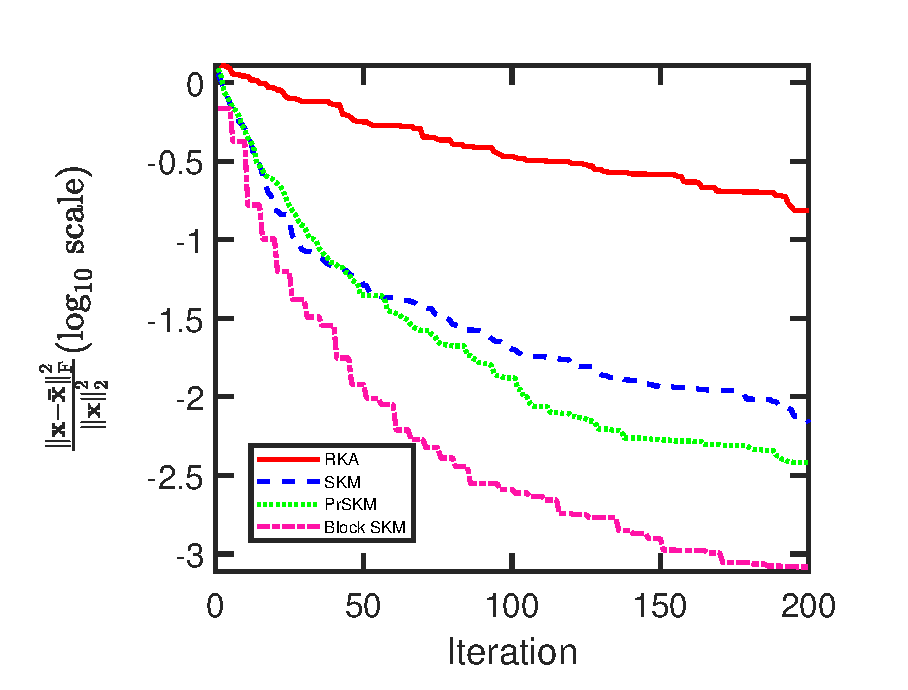
\includegraphics[width=0.47\columnwidth]{nmse_inequality.eps}}
	\caption{Comparing the 
 recovery performance of the two proposed Kaczmarz algorithms, namely the PrSKM and the Block SKM, with that of SKM and RKA for
 %: (a) a linear equation system, (b) 
 a linear inequality system. 
 \vspace{-15pt}
 }
	\label{figure_1}
\end{figure}
%-------------------------------------------------------

\section{Probabilistic Effect of Sample Abundance In One-Bit Sensing}
\label{ada_thresh_prob}
In Section~\ref{penalt}, we will introduce the concept of FVP and subsequently obtain the required number of one-bit samples $m^{\prime}$ to accurately capture the solution in the case of sample abundance, one-bit CS, and one-bit low-rank matrix recovery. In Section~\ref{error}, we will provide the convergence of ORKA based on the theoretical results obtained in Section~\ref{penalt}.
%An integral part of our proposed recovery algorithm is the RKA, whose recovery error was readily given in (\ref{eq:15}). In Section~\ref{error}, at first we will show that ORKA converges linearly in expectation to the nonempty feasible set \eqref{eq:80n} with the rate that depends on the sampling matrix $\mbA$.
%This fact will be shown in Theorem~\ref{theorem_2} by bridging the scaled condition number of matrices $\mbP$ and $\mbA$. Then, in Section~\ref{penalt}, we will derive a tight convergence bound for ORKA taking into account the effect of increasing the number of time-varying threshold sequences $m$. %Moreover, we will obtain some bounds on the required number of one-bit samples such that the recovered signal $\bar{\mbx}$ from the one-bit polyhedron \eqref{eq:80n} by ORKA falls inside the desired signal's ball space $\mathcal{B}_{r}(\mbx_{\star})$.
\begin{comment}
As was shown in \cite{strohmer2009randomized}, \Fr{in the case of linear system of equations such as $\mbA\mbx=\mbb$ with $\mbA\in\mathbb{R}^{m\times n}$ and $\mbb\in\mathbb{R}^{m}$,} the convergence rate of RKA does not depend on the number of equations $m$. \Fr{Similar conclusion has been made in the literature in the case of linear system of inequalities $\mbA\mbx\succeq\mbb$ \cite{leventhal2010randomized}. Note that our goal is to recover the signal $\bar{\mbx}$ in the polyhedron \eqref{eq:80n} which is as close as possible to the optimal signal $\mbx_{\star}$. Mathematically speaking, we are interested in the signal $\bar{\mbx}$ that is inside the desired signal's ball space with a small radius $r$; i.e. $\bar{\mbx}\in\mathcal{B}_{r}(\mbx_{\star})$. To achieve that,}
%in the system. 
%Nevertheless, when we face a non-linear constraint in our problem, as is generally the case in (\ref{eq:1nnnn}), it is desirable are made redundant by using the opportunity of having a large 
we are required to increase the number of samples in the polyhedron \eqref{eq:80n}, as typically provided via one-bit sampling, to make a non-linear constraint redundant in the original problem of interest. \textcolor{red}{we should cite the problem of interest here later.}
In such a case, the offered convergence rate \Fr{for the RKA (or its variants)} appears to be
%insufficient 
\Fr{not tight} since we must have enough number of samples to fulfill costly constraints (\Fr{or equivalently, we must have enough number of samples so that the finite-volume space created by the intersection of hyperplanes of \eqref{eq:80n} be inside the desired signal's ball space $\mathcal{B}_{r}(\mbx_{\star})$}). \Fr{As a result, to achieve a tighter convergence bound, an extra term as a \emph{penalty} must be considered alongside the derived bounds of the RKA (or its variants) to present the importance of sample size in our algorithm \cite{eamaz2022phase}.}

\Fr{To derive such sample-dependent penalty term for our convergence bound, we will rely on the average distances between the desired signal $\mbx_{\star}$ and its surrounding hyperplanes in \eqref{eq:80n}. The intuition behind our approach is that}
by adding more inequality constraints in (\ref{eq:80n}) as a result of extra one-bit samples, the shrinkage of the said polyhedron will put a downward pressure on the distance between the desired signal $\mathbf{x}_{\star}$ and its surrounding hyperplanes, each presenting an informative measurement that will shrink the feasibility space. As a result,
%We will show that 
by judicious sampling, the average of these distances will be bounded, which may be \Fr{alternatively} considered to model
%be 
a finite-volume space created around $\mathbf{x}_{\star}$. Moreover, \Fr{once the number of one-bit samples is enough such that the finite-volume space created by the intersection of hyperplanes in \eqref{eq:80n} be inside the desired signal's ball space $\mathcal{B}_{r}(\mbx_{\star})$,}
%as a result of using an overdetermined linear system of inequalities, 
the convergence of the RKA (or its variants) is guaranteed \Fr{to capture the local optima that is in the vicinity of the global optima of the original problem of interest} \cite{eamaz2022phase,leventhal2010randomized,needell2014paved,de2017sampling}.
\end{comment}

\subsection{Finite Volume Property}
\label{penalt}
%We derive the sample-dependent penalty function $\Upsilon\left(m^{\prime}\right)$ for the convergence rate of ORKA presented in \eqref{bound2}.
%We investigate the convergence of ORKA through a probabilistic lens. 
%To do so, assume that the $j$-th row of the matrix $\mbP$ in the one-bit polyhedron \eqref{eq:80n} is presented as $\left(\mbP\right)_{j}=r^{(\ell)}_{j^{\prime}}\mba_{_{j^{\prime}(j)}}$ with $\mba_{_{j^{\prime}(j)}}$ denotes the $j^{\prime}$-th row of the matrix $\mbA$, where $j^{\prime}(j)$ is defined as,
%\begin{equation}
%\label{Negindex} 
%\begin{aligned}
%j^{\prime}(j)=\begin{cases} \operatorname{mod}(j,n), & j\neq k n, \\ n, & j=k n,\end{cases}
%\end{aligned}
%\end{equation}
%with $1\leq k \leq m$. Similarly, the $j$-th element of $\operatorname{vec}\left(\mbR\right)\odot \operatorname{vec}\left(\bGamma\right)$ in the one-bit polyhedron is obtained as $\left(\operatorname{vec}\left(\mbR\right)\odot \operatorname{vec}\left(\bGamma\right)\right)_{j}=r^{(\ell)}_{j^{\prime}(j)}\tau^{(\ell)}_{j^{\prime}(j)}$.
Define the distance between the original signal $\mathbf{x}_{\star}$ and the $j$-th hyperplane presented in (\ref{eq:80n}) as 
\begin{equation}
\label{distance}
d^{(\ell)}_{j}\left(\mathbf{x}_{\star},\tau_{j}^{(\ell)}\right)=\left|r^{(\ell)}_{j}\mba_{_j}\mathbf{x}_{\star}-r^{(\ell)}_{j}\tau^{(\ell)}_{j}\right|,~j\in [n],~ \ell\in[m],%\mathcal{L},
\end{equation}\normalsize 
It is essential to clarify that in our analysis, we adopt the worst-case scenario for the distance between the desired point and the solutions. This approach considers the solution to lie precisely on the hyperplane. However, it is crucial to note that in reality, the solution to a linear inequality system can exist anywhere between the desired point and the hyperplane. \emph{It is easy to observe that by reducing the distances between $\mathbf{x}_{\star}$ and the constraint-associated hyperplanes in \eqref{eq:80n}, the possibility of capturing the original signal $\mbx_{\star}$ is increased.} For a specific sample size $m^{\prime}$, 
when $\operatorname{vol}\left(\mathcal{P}_{\mbx}\right)$ is reduced,
%when the volume of the finite space $\operatorname{vol}\left(\mathcal{P}_{\mbx}\right)$ (created by the hyperplanes in \eqref{eq:80n}) around the optimal point $\mbx_{\star}$ is reduced, 
the average of $\left\{d^{(\ell)}_{j}\left(\mathbf{x}_{\star},\tau_{j}^{(\ell)}\right)\right\}_{j,\ell=1}^{m^{\prime}}$ is diminished as well. This average of distances can be written as:
\begin{equation}
\label{ave}
\begin{aligned}
T_{\mathrm{ave}}=\frac{1}{m^{\prime}}\sum^{m^{\prime}}_{j,\ell=1}d^{(\ell)}_{j}\left(\mathbf{x}_{\star},\tau_{j}^{(\ell)}\right).
\end{aligned}
\end{equation}\normalsize
The one-bit phase retrieval problem, as investigated in \cite{eamaz2022phase}, derived a \emph{general Hoeffding's bound} \cite[Theorem~2.6.2]{vershynin2018high} to quantify the likelihood of achieving a finite volume and determine the necessary number of samples for one-bit signal reconstruction. In Theorem~\ref{theorem_0}, we utilize this result to address the problem of one-bit sensing. Specifically, we consider the distance between the original signal $\mbx_{\star}$ and the $j$-th hyperplane within the polyhedron defined in \eqref{eq:80n}, as described in \eqref{distance}.
%The possibility of creating a finite-volume, and the importance of the number of samples in the recovery performance of RKA, can be captured by the \emph{Chernoff bound} as illustrated below.
%\Fr{rewrite this based on the Hoeffding bound}
\begin{theorem}[Finite volume property (FVP)]
\label{theorem_0}
Assume the distances $\left\{d^{(\ell)}_{j}\left(\mathbf{x}_{\star},\tau^{(\ell)}_{j}\right)\right\}_{j,\ell=1}^{m^{\prime}}$ defined in \eqref{distance} between the desired point $\mathbf{x}_{\star}$ and the hyperplanes of the one-bit polyhedron \eqref{eq:80n} 
are %i.i.d. 
independent random variables with,
$\mathbb{E}\left\{T_{\mathrm{ave}}\right\}=\mu$ and $\left\|d^{(\ell)}_{j}\left(\mathbf{x}_{\star},\tau^{(\ell)}_{j}\right)\right\|_{\psi_{2}}^{2}\leq K$.
Then, based on the general Hoeffding's inequality, the probability of the finite volume created by hyperplanes lying within a ball $\mathcal{B}_\rho\left(\mbx_{\star}\right)$ centered at the original signal, with a radius of $\rho$, is bounded by:
\begin{equation}
\label{eq:theorem_cher}
\operatorname{Pr}\left(T_{\mathrm{ave}}\geq C \rho\right)\leq e^{\frac{-c_1\left(C\rho-\mu\right)^{2}}{K}m^{\prime}},
\end{equation}
where $C$ and $c_1$ are positive numbers. 
\end{theorem}
%The complete proof of deriving the bound in \eqref{eq:hoeffding_cher} can be found in the Appendix~\ref{A2}. 
%The MGF $\Psi_{_{T_{\mathrm{ave}}}}$ contains two parts. The first part has an increasing trend until a specific sample size $m^{\star}$, which indicates the existence of an abundant number of samples. After that, the function has a decreasing behavior. Therefore, $\Psi_{_{T_{\mathrm{ave}}}}$ with $m^{\prime}\geq m^{\star}$ can be a good choice for a sample size-dependent penalty function. Particularly, the penalty function can be chosen as $\Psi_{_{T_{\mathrm{ave}}}}-\Psi_{\infty}$, where $\Psi_{\infty}=\lim_{m^{\prime}\rightarrow \infty} \Psi_{_{T_{\mathrm{ave}}}}$, to ensure $\Upsilon(m^{\prime})\rightarrow 0$ as $m^{\prime}\rightarrow \infty$. 
Theorem~\ref{theorem_0} provides the probability of the finite volume, created by hyperplanes, being contained within the ball around the original signal. The positive number
%constant 
$C$ serves to consider the distances beyond the radius $\rho$ of the ball.
%(this value solely relies on the type of sub-Gaussianity exhibited by the sampling matrix and the time-varying thresholds). 
These distances correspond to ineffective hyperplanes that are incapable of forming a finite volume around the original signal. 
Mathematically, based on the general Hoeffding's inequality presented in \eqref{eq:theorem_cher}, it follows $\delta=C\rho-\mu$ for a positive constant $\delta$. We utilize this constant, $\delta$, in all the theoretical guarantees that will be obtained in this paper.
%, which leads to $C\geq\frac{\mu}{\rho}$. This informs that there exists a positive constant $c^{\prime}$ such that $C=\frac{\mu}{\rho}+c^{\prime}$, which results in $\delta=c^{\prime}\rho$. Therefore, one can replace $\delta=C\rho-\mu$ with $\delta=c^{\prime}\rho$ in all the theoretical guarantees that will be obtained in this paper.
In the remainder of the paper, our objective is to derive theoretical guarantees that enable us to achieve the uniform perfect reconstruction, as defined in the following definition: 
%Let $\mathcal{T}$ be a subset of $\mathbb{R}^n$, $\mathcal{T}\subseteq\mathbb{R}^n$. 
\begin{definition}[Uniform perfect reconstruction]
Uniform perfect reconstruction of a signal from one-bit polyhedron is achieved when all possible recovery solutions for $\bar{\mbx}\in\mathcal{P}_{\mbx}$ with 
\begin{equation}
\label{kumjun}
\operatorname{sgn}(\mba_j\mbx_{\star}-\tau_{j}^{(\ell)})=\operatorname{sgn}(\mba_j\bar{\mbx}-\tau_{j}^{(\ell)}),~j\in[n],~\ell\in[m],
\end{equation}
satisfy $\bar{\mbx}\in\mathcal{B}_\rho\left(\mbx_{\star}\right)$, for all $\mbx_{\star}$ in the space.
\end{definition}
Note that the sign preservation mentioned in our work, as stated in Definition~1, is equivalent to the solution provided by a linear feasibility solver, denoted as $\bar{\mbx}$, satisfying all the given inequalities, meaning $\bar{\mbx}\in\mathcal{P}_{\mbx}$. \emph{To fulfill Definition~1, it appears sufficient to acquire the number of samples that ensures the creation of a finite volume of intersections of hyperplanes with the maximum radius $\rho$}. This central idea underlies all of our theorems.
In the following theorem, we establish the minimum number of one-bit samples $m^{\prime}$ required in the sample abundance scenario to achieve an accurate recovery:
%to ensure that a solution $\bar{\mbx}$ lies within the ball space $\mathcal{B}_{\rho}\left(\mbx_{\star}\right)$ of the desired signal:

\begin{comment}
\Fr{To prove the bound in \eqref{eq:hoeffding_cher}, we use the following Lemma.
\begin{lemma}\cite[Lemma~1]{hoeffding1994probability}
\label{lemma_mgf}
If $X$ is a random variable such that $a\leq X\leq b$, then for any real number $t$
\begin{equation}
\label{eq:mgf}
\mathbb{E}\left\{e^{tX}\right\}\leq \frac{b-\mathbb{E}\left\{X\right\}}{b-a}e^{ta}+\frac{\mathbb{E}\left\{X\right\}-a}{b-a}e^{tb}.
\end{equation}
\end{lemma}
The complete proof of deriving the bound in \eqref{eq:hoeffding_cher} can be seen in the \textcolor{red}{Appendix}. Note that the decreasing bound in \eqref{eq:hoeffding_cher} is true when the distances $\left\{d^{(\ell)}_{j}\left(\mathbf{x}_{\star},\tau^{(\ell)}_{j^{\prime}(j)}\right)\right\}_{j,\ell=1}^{m^{\prime}}$ are all bounded (the second condition in \eqref{prop_dist}). For such cases of distances defined in $\eqref{distance}$ which the second condition in \eqref{prop_dist}, $0\leq d^{(\ell)}_{j}\left(\mathbf{x}_{\star},\tau^{(\ell)}_{j^{\prime}(j)}\right)\leq b$, is correct under an specific probability constraint, the bound \eqref{eq:hoeffding_cher} cannot be utilized in a straightforward manner. The example of this can be the case where each distance defined in \eqref{distance} follows the folded normal distribution; i.e. each term $r^{(\ell)}_{j^{\prime}(j)}\mba_{_{j^{\prime}(j)}}\mathbf{x}_{\star}-r^{(\ell)}_{j^{\prime}(j)}\tau^{(\ell)}_{j^{\prime}(j)}$ in \eqref{distance} has the normal distribution.
}
\end{comment}
%Note that the decreasing bound in \eqref{eq:hoeffding_cher} is true when the distances $\left\{d^{(\ell)}_{j}\left(\mathbf{x}_{\star},\tau^{(\ell)}_{j^{\prime}(j)}\right)\right\}_{j,\ell=1}^{m^{\prime}}$ are all bounded. While the condition $0\leq d^{(\ell)}_{j}\left(\mathbf{x}_{\star},\tau^{(\ell)}_{j^{\prime}(j)}\right)\leq b$ can be met with a specific probability constraint, the straightforward utilization of the bound \eqref{eq:hoeffding_cher} becomes challenging. A notable example is when each distance, as defined in \eqref{distance}, follows the folded normal distribution where each term $r^{(\ell)}_{j^{\prime}(j)}\mba_{_{j^{\prime}(j)}}\mathbf{x}_{\star}-r^{(\ell)}_{j^{\prime}(j)}\tau^{(\ell)}_{j^{\prime}(j)}$ in \eqref{distance} has the normal distribution. 
%For an arbitrary vector $\mbx\in\mathbb{R}^{d}$ generated as $\mbx\sim\mathcal{N}\left(\mathbf{0},\sigma^{2}\mbI\right)$, it has been shown that $\operatorname{Pr}\left(\left\|\mbx\right\|_{\infty}>\sqrt{2 \sigma^2 \log (d)}\right) \stackrel{d \rightarrow \infty}{\longrightarrow} 0$ \cite{leadbetter2012extremes}. This probabilistic bound can be employed to establish an expression for the bound of each distance $d^{(\ell)}_{j}\left(\mathbf{x}_{\star},\tau^{(\ell)}_{j^{\prime}(j)}\right)$ when they follow a folded normal distribution. 
%In order to address the concern associated with such examples, we will direct our attention to the MGF $\Psi_{T}$ itself, taking into account the Chernoff bound \eqref{eq:theorem_cher}. Specifically, we focus our analysis on Gaussian matrices, i.e., each element of the sensing matrix $\mbA$ 
%such that each element 
%is independently
%randomly 
%drawn from the standard Gaussian distribution, $\mathcal{N}(0,1)$. For these matrices, the required number of samples $m^{\prime}$ to capture the optimal solution $\mbx_{\star}$ in the one-bit polyhedron \eqref{eq:80n} is obtained from the FVP by the following theorem:
\begin{comment}
\begin{theorem}
\label{TH1}
Assume a $n\times d$ 
%Gaussian 
sensing matrix $\mbA=[a_{ij}]$ with $a_{ij}$ independently drawn from the standard Gaussian distribution, $\mathcal{N}(0,1)$, and the one-bit sampling matrix $\mbP=\Tilde{\bOmega}\mbA \in \mathbb{R}^{m^{\prime}\times d}$, where $m^{\prime}=mn$ denotes the total number of one-bit samples, and $m$ represents the number of time-varying sampling threshold sequences. The time-varying thresholds %$\uptau^{(\ell)}_{j}$ 
are generated according to $\left\{\tau^{(\ell)}_{j}\sim \mathcal{N}\left(0,\sigma^2\right)\right\}_{j,\ell=1}^{m^{\prime}}$. Consider a fixed $0<\eta< 1$ and $a=c\operatorname{vol}\left(\mathcal{B}_r\left(\mbx_{\star}\right)\right)$, where $\operatorname{vol}\left(\mathcal{B}_r\left(\mbx_{\star}\right)\right)=\frac{\left(\sqrt{\pi}r\right)^d}{\Gamma\left(\frac{d}{2}+1\right)}$ denotes the volume of a $d$-dimensional %volume of a 
ball with radius $r$ centered at the optimal solution $\mbx_{\star}$, and $c$ is a positive constant. If $\left\|\mbx_{\star}\right\|_{2}^{2}=M$, %the norm 2 of $\mbx$ is equal to $M$, 
then the minimum number of one-bit samples $m^{\prime}$ required to accurately capture a solution $\bar{\mbx}$ such that $\bar{\mbx}\in\mathcal{B}_r\left(\mbx_{\star}\right)$ with a probability higher than $1-\eta$ satisfies%inside the desired signal's ball, defined as
\begin{equation}
\label{numsample}
m^{\prime} \geq \frac{\left(M+\sigma^2\right)\ln\left(\frac{1}{\eta}\right)}{a^2-2\left(M+\sigma^2\right)\ln\left(2\right)}.
\end{equation}
\end{theorem}
The proof of Theorem~\ref{TH1} is discussed in Appendix~\ref{A3}. Note that when considering a small radius $r\leq 1$, the volume $\operatorname{vol}\left(\mathcal{B}_r\left(\mbx_{\star}\right)\right)$ decreases as the signal dimension $d$ grows sufficiently large. As a result, the right-hand side of \eqref{numsample} increases which means we require more number of one-bit samples $m^{\prime}$ to capture a solution $\bar{\mbx}$ such that $\bar{\mbx}\in\mathcal{B}_r\left(\mbx_{\star}\right)$ when the signal dimension $d$ increases.
\end{comment}
\begin{comment}
\begin{equation}
\label{ST-AR}
\mathcal{B}_r\left(\mbx\right) = \left\{\mbx\in\mathbb{R}^{d}\mid\left\|\mbx-\mbx_{\star}\right\|_2\leq r\right\},
\end{equation}
can be calculated as follows:
\end{comment}
%If we wish to move beyond the use of the Gaussian sampling matrix $\mbA$, it is possible to obtain the minimum number of
%necessary 
%one-bit samples $m^{\prime}$ in the sample abundance scenario under certain mild conditions. This is achieved by considering the following theorem:
\begin{theorem}
\label{TH10-ST}
Assume a $n\times d$ sampling matrix $\mbA$ such that each distance defined in \eqref{distance} is a
%an unbounded 
sub-Gaussian random variable,
%with $\mathbb{E}\left\{T_{\mathrm{ave}}\right\}=\mu$ and $\left\|d^{(\ell)}_{j}\left(\mathbf{x}_{\star},\tau^{(\ell)}_{j}\right)\right\|_{\psi_{2}}^{2}\leq K$
and the one-bit sampling matrix $\mbP=\Tilde{\bOmega}\mbA \in \mathbb{R}^{m^{\prime}\times d}$, where $m^{\prime}=mn$ denotes the total number of one-bit samples, and $m$ represents the number of time-varying sampling threshold sequences. %Define the set $\mathcal{T}=\left\{\mbx\in\mathbb{R}^d\mid\|\mbx\|_2\leq 1\right\}$. 
Denote $\delta$ and $C_1$ as positive constants. 
%and $0<\rho<1$.
%and $C$ is a positive constant.
%Consider a fixed $0<\eta< 1$ %and $cr>\mu$ %$a=c\operatorname{vol}\left(\mathcal{B}_r\left(\mbx_{\star}\right)\right)$, 
%and $\rho$ %$\operatorname{vol}\left(\mathcal{B}_r\left(\mbx_{\star}\right)\right)=\frac{\left(\sqrt{\pi}r\right)^d}{\Gamma\left(\frac{d}{2}+1\right)}$ 
%to be the radius
%volume 
%of a $d$-dimensional ball $\mathcal{B}_\rho\left(\mbx_{\star}\right)$ %with radius $r$ 
%centered at the optimal solution $\mbx_{\star}$.
%For a positive absolute constant $C_1$, 
If the number of one-bit samples obeys
\begin{equation}
\label{goodarz}
m^{\prime}\geq C_1\delta^{-2}\left(\frac{3d}{\rho}+\log\left(\frac{1}{\eta}\right)\right), 
\end{equation}
then with a probability of at least $1-\eta$, we achieve the uniform perfect reconstruction with $\bar{\mbx}\in\mathcal{B}_\rho\left(\mbx_{\star}\right)$.
%the minimum number of one-bit samples $m^{\prime}$ required to accurately capture a solution $\bar{\mbx}$ such that $\bar{\mbx}\in\mathcal{B}_\rho\left(\mbx_{\star}\right)$ with a probability higher than $1-\eta$ satisfies
\begin{comment}
\begin{equation}
\label{goodarz}
m^{\prime}\geq\frac{K\ln\left(\frac{1}{\eta}\right)}{c_{1}\left(C \rho-\mu\right)^2}.
\end{equation}\normalsize
\end{comment}
\end{theorem}
The proof of Theorem~\ref{TH10-ST} is presented in Appendix~\ref{ealmaz}.
%The condition stated in \eqref{kumjun} is commonly referred to as the \emph{consistent reconstruction} in one-bit settings in prior literature
%The condition in \eqref{kvm_27} is called the \emph{consistent reconstruction} in one-bit settings in previous literature 
%\cite{baraniuk2017exponential,jacques2013robust,laska2011trust,boufounos20081}.
%simply proved considering the bound \eqref{eq:theorem_cher}. %Note that the effect of signal dimension $d$ on the right-hand side of \eqref{goodarz} is concealed within the variables $\mu$ and $K$. 
%In the supplementary material, we delve deeper into the exploration of the optimal sample count for dithered one-bit sensing. Specifically, we focus on analyzing the cases of the DCT sampling matrix $\mbA$ and uniform dither. The Gaussian sampling matrix with Gaussian dithering scheme is also comprehensively investigated in the supplementary material.
Following the discussion provided in \cite{xu2020quantized} regarding the benefit of uniform dithering in the case of bounded measurements, the Corollary~\ref{uniform_dither} presents the result of Theorem~\ref{TH10-ST} in the case of the DCT sensing matrix $\mbA$ and uniform dither:
\begin{corollary}
\label{uniform_dither}
Consider 
%the settings in Theorem~\ref{TH10-ST} with 
a $n\times d$ DCT matrix $\mbA$, and the time-varying thresholds which
are generated according to $\left\{\tau^{(\ell)}_{j}\sim \mathcal{U}\left(-\bt,\bt\right)\right\}_{j,\ell=1}^{m^{\prime}}$ such that $\bt>0$. 
%Assume that 
Denote $f_j$ as the $j$-th DCT coefficient of $\mbx_{\star}$.
%optimal solution 
%with the constraint $\left\|\mbx_{\star}\right\|_{\infty}\leq M$. 
%For a positive constant $\delta$, 
If we have
%Then for a positive constant $C$, the minimum number of one-bit samples $m^{\prime}$ required to accurately capture a solution $\bar{\mbx}$ from the one-bit DCT coefficients such that $\bar{\mbx}\in\mathcal{B}_{\rho}\left(\mbx_{\star}\right)$ with a probability higher than $1-\eta$ satisfies
\begin{equation}
\label{kvm_3}
m^{\prime}\geq \frac{1}{2}\delta^{-2}\left(\bt+\sqrt{2}\right)^2\left(\frac{3d}{\rho}+\log\left(\frac{1}{\eta}\right)\right),%\frac{\left(\sqrt{2d}M+\bt\right)\ln\left(\frac{1}{\eta}\right)}{2(C\rho-\mu)^2},
\end{equation}
then with a probability of at least $1-\eta$, we achieve the uniform perfect reconstruction with
%for all $\mbx_{\star}$, all possible recovery solutions $\bar{\mbx}$ with the consistent reconstruction criterion \eqref{kumjun} satisfy 
$\bar{\mbx}\in\mathcal{B}_\rho\left(\mbx_{\star}\right)$,
%where $\delta=C\rho-\mu$ is a constant which is fixed over the signal dimension $d$, 
and $\delta=C\rho-\mu$ for a positive value $C$ with
\begin{equation}
\label{kvm_4}
\begin{aligned}
\mu=\frac{1}{2\bt n}&\sum_{j=1}^{n}I(-\bt\leq f_j\leq\bt)\left(f_{j}^2+\bt^2\right)\\&+I(f_j\geq\bt)(2\bt f_j)+I(f_j\leq-\bt)(-2\bt f_j).
\end{aligned}
\end{equation}
\end{corollary}
The proof of Corollary~\ref{uniform_dither} is presented in Appendix~\ref{kvm_5}. In the following corollary, we present the result of Theorem~\ref{TH10-ST} for the Gaussian sampling matrix with Gaussian dithering scheme:
%when each term $r^{(\ell)}_{j}\mba_{_{j}}\mathbf{x}_{\star}-r^{(\ell)}_{j}\tau^{(\ell)}_{j}$ in \eqref{distance} follows the normal distribution:
\begin{corollary}
\label{jennifer}
Consider 
%the settings in Theorem~\ref{TH10-ST} with 
a $n\times d$ sampling matrix $\mbA=[a_{ij}]$ with $a_{ij}$ independently drawn from the standard Gaussian distribution, $\mathcal{N}(0,1)$, and
%and the one-bit sampling matrix $\mbP=\Tilde{\bOmega}\mbA \in \mathbb{R}^{m^{\prime}\times d}$, where $m^{\prime}=mn$ denotes the total number of one-bit samples, and $m$ represents the number of time-varying sampling threshold sequences. 
the time-varying thresholds which %$\uptau^{(\ell)}_{j}$ 
are generated according to $\left\{\tau^{(\ell)}_{j}\sim \mathcal{N}\left(0,\sigma^2\right)\right\}_{j,\ell=1}^{m^{\prime}}$. %Consider a fixed $0<\eta< 1$ and $a=c\operatorname{vol}\left(\mathcal{B}_r\left(\mbx_{\star}\right)\right)$, where $\operatorname{vol}\left(\mathcal{B}_r\left(\mbx_{\star}\right)\right)=\frac{\left(\sqrt{\pi}r\right)^d}{\Gamma\left(\frac{d}{2}+1\right)}$ denotes the volume of a $d$-dimensional %volume of a ball with radius $r$ centered at the optimal solution $\mbx_{\star}$, and $c$ is a positive constant. 
%If $\left\|\mbx_{\star}\right\|_{\infty}\leq M$, for positive constants $C$ and $C^{\prime}$
%$c^{\prime}$ and $\Tilde{c}$ 
%the minimum number of one-bit samples $m^{\prime}$ required to accurately capture a solution $\bar{\mbx}$ such that $\bar{\mbx}\in\mathcal{B}_{\rho}\left(\mbx_{\star}\right)$ with a probability higher than $1-\eta$ satisfies
If we have
\begin{equation}
\label{jen_1}
m^{\prime}\geq C_1\delta^{-2}\left(\sigma^2+1\right)\left(\frac{3d}{\rho}+\log\left(\frac{1}{\eta}\right)\right),
%\left(dM^2+\sigma^2\right)\log\left(\frac{1}{\eta}\right),
%\frac{c^{\prime}\sqrt{dM^2+\sigma^2}\ln\left(\frac{1}{\eta}\right)}{\left(\Tilde{c}r-\sqrt{\frac{2}{\pi}\left(dM^2+\sigma^2\right)}\right)^2}.
\end{equation}
then with a probability of at least $1-\eta$, we achieve the uniform perfect reconstruction with $\bar{\mbx}\in\mathcal{B}_\rho\left(\mbx_{\star}\right)$, and $\delta=C\rho-\mu$ for a positive value $C$ with
%where $\delta=C\rho-\mu$ is a constant which is fixed over the signal dimension $d$, and 
$\mu\leq\sqrt{\frac{2}{\pi}\left(\sigma^2+1\right)}$.
\end{corollary}
The proof of Corollary~\ref{jennifer} is presented in Appendix~\ref{A6}.
\begin{comment}
\begin{corollary}
\label{uniform_dither}
Consider the settings in Theorem~\ref{TH10-ST} with a $n\times d$ DCT matrix $\mbA$, and the time-varying thresholds which
are generated according to $\left\{\tau^{(\ell)}_{j}\sim \mathcal{U}\left(-\bt,\bt\right)\right\}_{j,\ell=1}^{m^{\prime}}$ such that $\bt>0$. Assume that $\mbx_{\star}$ is a nonnegative optimal solution with the constraint $\left\|\mbx_{\star}\right\|_{\infty}\leq M$. Denote $f_j$ as the $j$-th DCT coefficient of $\mbx_{\star}$. Then for a positive constant $c>1$, the minimum number of one-bit samples $m^{\prime}$ required to accurately capture a solution $\bar{\mbx}$ such that $\bar{\mbx}\in\mathcal{B}_r\left(\mbx_{\star}\right)$ with a probability higher than $1-\eta$ satisfies
\begin{equation}
\label{kvm_3}
m^{\prime}\geq \frac{\left(\sqrt{2d}M+\bt\right)\ln\left(\frac{1}{\eta}\right)}{2(cr-\mu)^2},
\end{equation}
where $\mu$ is
\begin{equation}
\label{kvm_4}
\begin{aligned}
\mu=\frac{1}{2\bt n}&\sum_{j=1}^{n}I(-\bt\leq f_j\leq\bt)\left(f_{j}^2+\bt^2\right)\\&+I(f_j\geq\bt)(2\bt f_j)+I(f_j\leq-\bt)(-2\bt f_j).
\end{aligned}
\end{equation}
\end{corollary}
The proof of Corollary~\ref{uniform_dither} is presented in Appendix~\ref{kvm_5}. Note that the decreasing bound in \eqref{eq:hoeffding_cher} is true when the distances $\left\{d^{(\ell)}_{j}\left(\mathbf{x}_{\star},\tau^{(\ell)}_{j^{\prime}(j)}\right)\right\}_{j,\ell=1}^{m^{\prime}}$ are all bounded. While the condition $0\leq d^{(\ell)}_{j}\left(\mathbf{x}_{\star},\tau^{(\ell)}_{j^{\prime}(j)}\right)\leq b$ can be met with a specific probability constraint, the straightforward utilization of the bound \eqref{eq:hoeffding_cher} becomes challenging. A notable example is when each distance, as defined in \eqref{distance}, follows the folded normal distribution where each term $r^{(\ell)}_{j^{\prime}(j)}\mba_{_{j^{\prime}(j)}}\mathbf{x}_{\star}-r^{(\ell)}_{j^{\prime}(j)}\tau^{(\ell)}_{j^{\prime}(j)}$ in \eqref{distance} has the normal distribution. The following Theorem provides the minimum number of one-bit samples $m^{\prime}$ for such scenarios:

This Theorem can be simply proved by a minor modification to the general Hoeffding's inequality \cite[Theorem~2.6.2]{vershynin2018high}. Note that the effect of signal dimension $d$ on the right-hand side of \eqref{goodarz} is hidden within the variables $\mu$ and $K$. In the following corollary, we present the result of Theorem~\ref{prob_distance} when each term $r^{(\ell)}_{j^{\prime}(j)}\mba_{_{j^{\prime}(j)}}\mathbf{x}_{\star}-r^{(\ell)}_{j^{\prime}(j)}\tau^{(\ell)}_{j^{\prime}(j)}$ in \eqref{distance} follows the normal distribution:
\begin{corollary}
\label{jennifer}
Consider the settings in Theorem~\ref{prob_distance} with a $n\times d$ sensing matrix $\mbA=[a_{ij}]$ with $a_{ij}$ independently drawn from the standard Gaussian distribution, $\mathcal{N}(0,1)$, and
%and the one-bit sampling matrix $\mbP=\Tilde{\bOmega}\mbA \in \mathbb{R}^{m^{\prime}\times d}$, where $m^{\prime}=mn$ denotes the total number of one-bit samples, and $m$ represents the number of time-varying sampling threshold sequences. 
the time-varying thresholds which %$\uptau^{(\ell)}_{j}$ 
are generated according to $\left\{\tau^{(\ell)}_{j}\sim \mathcal{N}\left(0,\sigma^2\right)\right\}_{j,\ell=1}^{m^{\prime}}$. %Consider a fixed $0<\eta< 1$ and $a=c\operatorname{vol}\left(\mathcal{B}_r\left(\mbx_{\star}\right)\right)$, where $\operatorname{vol}\left(\mathcal{B}_r\left(\mbx_{\star}\right)\right)=\frac{\left(\sqrt{\pi}r\right)^d}{\Gamma\left(\frac{d}{2}+1\right)}$ denotes the volume of a $d$-dimensional %volume of a ball with radius $r$ centered at the optimal solution $\mbx_{\star}$, and $c$ is a positive constant. 
If $\left\|\mbx_{\star}\right\|_{\infty}\leq M$, for positive values $c^{\prime}$ and $\Tilde{c}$ the minimum number of one-bit samples $m^{\prime}$ required to accurately capture a solution $\bar{\mbx}$ such that $\bar{\mbx}\in\mathcal{B}_r\left(\mbx_{\star}\right)$ with a probability higher than $1-\eta$ satisfies
\begin{equation}
\label{jen_1}
m^{\prime}\geq\frac{c^{\prime}\sqrt{dM^2+\sigma^2}\ln\left(\frac{1}{\eta}\right)}{\left(\Tilde{c}r-\sqrt{\frac{2}{\pi}\left(dM^2+\sigma^2\right)}\right)^2}.
\end{equation}
\end{corollary}
The proof of Corollary~\ref{jennifer} is discussed in Appendix~\ref{A6}. Later in Section~\ref{ada_thresh}, we will utilize Theorem~\ref{prob_distance} to statistically design the threshold parameters. Note that the Hoeffding's inequality for bounded random variables \cite[Theorem~2]{hoeffding1994probability} can be deduced from the general Hoeffding's inequality for sub-Gaussian random variables \cite[Theorem~2.6.2]{vershynin2018high}. Therefore, we derive the sample size-dependent penalty function $\Upsilon\left(m^{\prime}\right)$ for ORKA in the sample abundance scenario based on Theorem~\ref{prob_distance}.
\end{comment}
%Considering the assumptions provided in Theorem~\ref{TH10-ST}, $\mathbb{E}\left\{T_{\mathrm{ave}}\right\}=\mu$ and $\left\|d^{(\ell)}_{j}\left(\mathbf{x}_{\star},\tau^{(\ell)}_{j}\right)\right\|_{\psi_{2}}^{2}\leq K$, we present the sample size-dependent penalty function $\Upsilon\left(m^{\prime}\right)$ in the following Proposition:
%\begin{proposition}
%\label{Penalty for Stephanie}   
%The appropriate choice for the sample size-dependent penalty function $\Upsilon\left(m^{\prime}\right)$ can be determined by considering the convergence rate of ORKA in the sample abundance scenario \eqref{bound2} and the settings provided in Theorem~\ref{TH10-ST} with positive constant values $c>1$, $c_1$ and $c_2$, as follows:
%\begin{equation}
%\label{ST?}
%\Upsilon\left(m^{\prime}\right)=c_2\left(e^{-\frac{c_1 m^{\prime} \left(C \rho-\mu\right)^2}{K}}-\eta\right)^{+},
%\end{equation}\normalsize
%with a probability higher than $1-\eta$.
%\end{proposition}
%Based on our discussion in Proposition~\ref{penaltyyy}, the penalty function $\Upsilon\left(m^{\prime}\right)$ should satisfy $\Upsilon\left(m^{\prime}\right)\rightarrow 0$ when $\operatorname{vol}\left(\mathcal{P}_{\mbx}\right)\subset\operatorname{vol}\left(\mathcal{B}_{\rho}(\mbx_{\star})\right)$. Based on Theorem~\ref{TH10-ST}, once the number of one-bit samples $m^{\prime}$ satisfies the bound \eqref{goodarz}, one can achieve the solution $\bar{\mbx}$ such that $\bar{\mbx}\in\mathcal{B}_\rho\left(\mbx_{\star}\right)$ with a probability at least $1-\eta$. This also informs that with such number of one-bit samples $m^{\prime}$ in \eqref{goodarz}, $\operatorname{vol}\left(\mathcal{P}_{\mbx}\right)\subset\operatorname{vol}\left(\mathcal{B}_{\rho}(\mbx_{\star})\right)$ with a probability at least $1-\eta$. As a result, with such probability and the number of one-bit samples $m^{\prime}$, the penalty function $\Upsilon\left(m^{\prime}\right)$ in \eqref{ST?} approaches zero. It is easy to verify that when the distances defined in \eqref{distance} are bounded random variables, $0\leq d^{(\ell)}_{j}\left(\mathbf{x}_{\star},\tau^{(\ell)}_{j}\right)\leq b$, then based on Hoeffding's inequality \cite[Theorem~2]{hoeffding1994probability}, the penalty function $\Upsilon\left(m^{\prime}\right)$ takes the form $\Upsilon\left(m^{\prime}\right)=c_2\left(e^{-\frac{2 m^{\prime} \left(C\rho-\mu\right)^2}{b^2}}-\eta\right)^{+}$ with a probability higher than $1-\eta$. The discussion about the required number of iterations for ORKA to obtain an upper recovery bound $\mathbb{E}\left\{\left\|\mbx_{i+1}-\mbx_{\star}\right\|^2_2\right\}\leq \epsilon_0$ in the sample abundance scenario can be found in Section~F of the Supplementary Material.
%The proof of this corollary is presented in Section F of the Supplementary Material. 
It is important to note that in the absence of dithering, creating a finite volume around the desired solution becomes impossible, rendering the FVP ineffective. Furthermore, in such scenarios, certain information, such as the signal amplitude, may be lost. However, in specific circumstances where the signal is $s$-sparse and confined within a unit ball, some sampling theorems have been derived in the literature \cite[Theorem~2]{jacques2013robust}.

The existing literature provides numerous theoretical derivations for the case where the input signal possesses an $s$-sparse structure, primarily focusing on the zero threshold scenario (e.g., \cite[Theorem~2]{jacques2013robust}). However, in order to determine the minimum number of samples required for achieving perfect reconstruction of sparse signals, we need to introduce the distance within the $s$-dimensional space. Let us consider an $s$-support column-submatrix of the sampling matrix, denoted as $\mathbf{A}_s$. The rows of this submatrix are represented by $\mathbf{a}^{(s)}_j$. Additionally, we have an $s$-subvector of $\mathbf{x}_\star$, denoted as $\mathbf{x}^{(s)}_\star$. The distances between the $s$-sparse original signal and the hyperplanes are given by
\begin{equation}
\label{distance_st}
d^{(\ell)s}_{j}\left(\mathbf{x}_{\star}^{(s)},\tau_{j}^{(\ell)}\right)=\left|r^{(\ell)}_{j}\mba^{(s)}_{_{j}}\mathbf{x}_{\star}^{(s)}-r^{(\ell)}_{j}\tau^{(\ell)}_{j}\right|,\quad s\in [d]. 
\end{equation}\normalsize
It is important to note that for a $s$-sparse signal, we have a total of $\binom{d}{s}$ 
%$\left(\begin{array}{c}d\\s\end{array}\right)$ 
possible choices for the distances. In other words, in the case of a $s$-support problem, we can select $\binom{d}{s}$ %$\left(\begin{array}{c}d\\s\end{array}\right)$ 
different submatrices $\mathbf{A}_s$ from the sampling matrix. By utilizing the general Hoeffding's inequality along with the union bound for these $\binom{d}{s}$
%$\left(\begin{array}{c}d\\s\end{array}\right)$ 
possibilities, the following theorem provides the necessary number of one-bit samples to achieve uniform perfect reconstruction of a $s$-sparse signal:
\begin{theorem}
\label{TH10-Stephania}
Assume a $n\times d$ sampling matrix $\mbA$ such that each distance defined in \eqref{distance_st} is a
%an unbounded 
sub-Gaussian random variable. Assume that the desired signal is $s$-sparse and $\rho$ is the radius of a ball centered at the original signal $\mbx_{\star}\in\mathbb{R}^{d}$. Consider a fixed $0<\eta< 1$ %and $cr>\mu$ %$a=c\operatorname{vol}\left(\mathcal{B}_r\left(\mbx_{\star}\right)\right)$, 
and $\delta_s$ %$\operatorname{vol}\left(\mathcal{B}_r\left(\mbx_{\star}\right)\right)=\frac{\left(\sqrt{\pi}r\right)^d}{\Gamma\left(\frac{d}{2}+1\right)}$ 
to be a positive constant value.  
%For a positive value $c_1$, 
Then the minimum number of one-bit samples $m^{\prime}$ required to accurately capture a $s$-sparse solution $\bar{\mbx}$, satisfies
\begin{equation}
\label{goodarz_1}
m^{\prime}\geq\delta_s\left(\log\left(\frac{1}{\eta}\right)+s\left(\log\left(\frac{ed}{s}\right)+\frac{3}{\rho}\right)\right),
\end{equation}\normalsize
with a probability higher than $1-\eta$. 
\end{theorem}
The proof of Theorem~\ref{TH10-Stephania} is provided in Appendix~\ref{arian}. 
In the following corollary, we provide the result of Theorem~\ref{TH10-Stephania} in the case of Gaussian sensing matrix with a Gaussian dithering scheme:
\begin{corollary}
\label{kvm_35}
Assume a $n\times d$ sampling matrix $\mbA=[a_{ij}]$ with $a_{ij}$ independently drawn from the standard Gaussian distribution, $\mathcal{N}(0,1)$, and the time-varying thresholds which %$\uptau^{(\ell)}_{j}$ 
are generated according to $\left\{\tau^{(\ell)}_{j}\sim \mathcal{N}\left(0,\sigma^2\right)\right\}_{j,\ell=1}^{m^{\prime}}$. Define the set $\mathcal{H}_{d,s}$ as
\begin{equation}
\label{kvm_36}
\mathcal{H}_{d,s}=\left\{\mbx\in\mathbb{R}^{d}\mid\|\mbx\|_1\leq\sqrt{s},\|\mbx\|_2\leq 1\right\},
\end{equation}
with $s\ll d$. Denote $\delta=C\rho-\sqrt{\frac{2}{\pi}(\sigma^2+1)}$ for a positive value $C$ and $0<\rho<1$. For a positive constant $C_1$, if $m^{\prime}\geq C_1\delta^{-2}(\sigma^2+1)\left(\log\left(\frac{1}{\eta}\right)+s\left(\log\left(\frac{ed}{s}\right)+\frac{3}{\rho}\right)\right)$, then with probability of at least $1-\eta$, and for all $\mbx_{\star},\bar{\mbx}\in\mathcal{H}_{d,s}$ we achieve the uniform perfect reconstruction with $\bar{\mbx}\in\mathcal{B}_\rho\left(\mbx_{\star}\right)$.
\begin{comment}
for all $\mbx_{\star}\in\mathcal{H}_{d,s}$, all possible recovery solutions $\bar{\mbx}\in\mathcal{H}_{d,s}$ with
\begin{equation}
\label{kvm_37}
\operatorname{sgn}(\mba_j\mbx_{\star}-\tau_{j}^{(\ell)})=\operatorname{sgn}(\mba_j\bar{\mbx}-\tau_{j}^{(\ell)}),~j\in[n],~\ell\in[m],
\end{equation}
satisfy $\|\mbx_{\star}-\bar{\mbx}\|_2\leq\rho$. The positive constant $C_1$ is an absolute constant.
\end{comment}
\end{corollary}
The proof of Corollary~\ref{kvm_35} follows directly from the proof of Theorem~\ref{TH10-Stephania} and the proof of Corollary~\ref{jennifer}. To investigate the necessary number of one-bit samples for $r$-rank matrices, one can identify a value $k \in [K]$ from a set of $K$ possibilities, such that $\mathbf{X}_k$ lies within a ball centered at the original signal with a radius of $\rho$. Assume $n_1=n_2$, previous studies, such as \cite[Lemma~3.1]{candes2011tight}, have demonstrated that $K$ satisfies the inequality $K \leq (1 + \frac{6}{\rho})^{(2n_1+1)r}$. By combining the general Hoeffding's inequality with the union bound applied to all $K$ possibilities, we can establish the following theorem:
\begin{theorem}
\label{TH10-Stephania❤️}
Assume a $n\times n^2_1$ sampling matrix $\mbA$ such that each distance defined in \eqref{distance} is a
%an unbounded 
sub-Gaussian random variable. Assume that the desired signal is $r$-rank matrix and $\rho$ is the radius of a ball centered at the original signal $\mbX_{\star}\in\mathbb{R}^{n_1\times n_1}$. Consider a fixed $0<\eta< 1$ %and $cr>\mu$ %$a=c\operatorname{vol}\left(\mathcal{B}_r\left(\mbx_{\star}\right)\right)$, 
and $\delta_r$ %$\operatorname{vol}\left(\mathcal{B}_r\left(\mbx_{\star}\right)\right)=\frac{\left(\sqrt{\pi}r\right)^d}{\Gamma\left(\frac{d}{2}+1\right)}$ 
to be a positive constant value.  
%For a positive value $c_1$, 
Then the minimum number of one-bit samples $m^{\prime}$ required to precisely capture a $r$-rank solution, satisfies
\begin{equation}
\label{goodarz_2}
m^{\prime}\geq\delta_r\left(\frac{18 n_1 r}{\rho}+\log\left(\frac{1}{\eta}\right)\right),
\end{equation}\normalsize
with a probability higher than $1-\eta$.
\end{theorem}
The proof of Theorem~\ref{TH10-Stephania❤️} is provided in Appendix~\ref{soli}. In the following corollary, we provide the result of Theorem~\ref{TH10-Stephania❤️} in the case of Gaussian sensing matrix with a Gaussian dithering scheme:
\begin{corollary}
\label{kvm_53}
Assume a $n\times n_1^2$ sampling matrix $\mbA=[a_{ij}]$ with $a_{ij}$ independently drawn from the standard Gaussian distribution, $\mathcal{N}(0,1)$,
%Let each element of $\left\{\mbA_j\in\mathbb{R}^{n\times n}\right\}_{j=1}^{n}$ be independently drawn from the standard normal distribution. Assume 
and the time-varying thresholds which are generated according to $\left\{\tau^{(\ell)}_{j}\sim \mathcal{N}\left(0,\sigma^2\right)\right\}_{j,\ell=1}^{m^{\prime}}$. Define the set $\mathcal{K}_{n_1,r}$ as
\begin{equation}
\label{boz}
\mathcal{K}_{n_1,r}=\left\{\mbX\in\mathbb{R}^{n_1\times n_1}\mid \operatorname{rank}(\mbX)\leq r,\|\mbX\|_{\mathrm{F}}\leq 1\right\}.
\end{equation}
Denote $\delta=C\rho-\sqrt{\frac{2}{\pi}(\sigma^2+1)}$ for a positive value $C$ and $0<\rho<1$. For a positive constant $C_1$, if $m^{\prime}\geq C_1\delta^{-2}(\sigma^2+1)\left(\frac{18n_1r}{\rho_r}+\log\left(\frac{1}{\eta}\right)\right)$, then with a probability of at least $1-\eta$, and for all $\mbX_{\star},\bar{\mbX}\in\mathcal{K}_{n_1,r}$, we achieve the uniform perfect reconstruction with $\bar{\mbX}\in\mathcal{B}_\rho\left(\operatorname{vec}\left(\mbX_{\star}\right)\right)$.
\begin{comment}
defined in \eqref{kvm_45}, all possible recovery solutions $\bar{\mbX}\in\mathcal{K}_{n,r}$ with

\begin{equation}
\label{kvm_54}
\operatorname{sgn}\left(\operatorname{Tr}\left(\mbA_j^{\top}\mbX_{\star}\right)-\tau_j^{(\ell)}\right)=\operatorname{sgn}\left(\operatorname{Tr}\left(\mbA_j^{\top}\bar{\mbX}\right)-\tau_j^{(\ell)}\right),j\in[n],\ell\in[m],
\end{equation} \normalsize
satisfy $\|\mbX_{\star}-\bar{\mbX}\|_{\mathrm{F}}\leq\rho$. The positive constant $C_1$ is an absolute constant.
\end{comment}
\end{corollary}
The proof of Corollary~\ref{kvm_53} follows directly from the proof of Theorem~\ref{TH10-Stephania❤️} and the proof of Corollary~\ref{jennifer}. As per the aforementioned theorems, the specific structure of the signal, such as sparsity or low-rank, has a direct impact on the probability of creating a finite volume around the original signal using one-bit hyperplanes. This structural characteristic manifests itself in the required number of samples for achieving accurate reconstruction. Note that Theorems~\ref{TH10-ST}, \ref{TH10-Stephania}, and \ref{TH10-Stephania❤️} present uniform reconstruction results, indicating that with high probability, all vectors can be reconstructed. This differs from a nonuniform result where each vector is individually reconstructed with high probability.

To have a robust recovery performance in one-bit signal sensing, it is necessary to design the time-varying thresholds such that the dynamic range (DR) of such thresholds covers the DR of the high-resolution measurements. In the following proposition,
%Herein, 
we focus our analysis to the sub-Gaussian
%standard normal 
sensing matrix with both Gaussian and Uniform dithering:
%where the result is presented in the following Proposition:
%(similar to the settings in Corollary~\ref{kvm_35} and Corollary~\ref{kvm_53}). 
%The following lemma provides how to design the standard deviation of the Gaussian dither in this scenario:
\begin{lemma}
\label{kvm_57}
Assume a $n\times d$ sub-Gaussian sensing matrix $\mbA$ with the rows $\{\mba_j\}_{j=1}^{n}$ 
%with $a_{ij}$ independently drawn from the standard Gaussian distribution, $\mathcal{N}(0,1)$, 
and the time-varying thresholds which %$\uptau^{(\ell)}_{j}$ 
are generated according to $\left\{\tau_{j}^{g}\sim \mathcal{N}\left(0,\sigma^2\right)\right\}_{j=1}^{n}$ and $\left\{\tau_{j}^{u}\sim \mathcal{U}\left(-\Tilde{b},\Tilde{b}\right)\right\}_{j=1}^{n}$. The high-resolution measurements are represented as $\mby=\mbA\mbx$. Define $K=\max_j\|\mba_j\mbx\|_{\psi_2}$. If $\|\mbx\|_2\leq R$, then setting $\sigma=\mathcal{O}\left(\sqrt{\frac{3}{8}}K R\right)$ in the Gaussian dither and  $\Tilde{b}=\mathcal{O}\left(\log(2) KR\right)$ in the Uniform dither guarantee the cover of $\mathrm{DR}_{\mby}$.
\end{lemma}
The proof of Lemma~\ref{kvm_57} is presented in Appendix~\ref{fy}. In the case of the Gaussian sensing matrix $\mbA=[a_{ij}]$ with $a_{ij}$ independently drawn from the standard Gaussian distribution, $\mathcal{N}(0,1)$, the result of Lemma~\ref{kvm_57}
%this result 
is simplified to $\sigma=\mathcal{O}(R)$ in the Gaussian dither and $\Tilde{b}=\mathcal{O}\left(R\log(2)\sqrt{\frac{8}{3}}\right)$ in the Uniform dither. For the example provided in Corollary~\ref{uniform_dither} regarding the DCT sampling matrix and uniform dithering, we should have $\bt=\mathcal{O}(\sqrt{2})$ to cover the DR of high-resolution measurements (DCT coefficients). The reason behind this can be seen in the proof of Corollary~\ref{uniform_dither}.

\subsection{Recovery Error Upper Bound for ORKA}
\label{error}
As the scaled condition number is the central parameter governing the recovery error of the RKA or its variants, in the following theorem we will evaluate the scaled condition number of the matrix $\mbP$ defined in \eqref{eq:90} to unveil the connection between the convergence bounds of the RKA (or its variants) and ORKA.
%it for ORKA-created matrix $\mbP$ in the following, starting with $\sigma_{min}$. The singular values of $\mbP$ may be determined based on the following theorem, which thus unveils the value of $\sigma_{min}$.
\begin{theorem}
\label{theorem_2}
Consider the one-bit polyhedron \eqref{eq:80n} associated with the linear system of equations $\mbA\mbx=\mby$ with $\mbA\in\mathbb{R}^{n\times d}$ and $m$ denotes the number of time-varying sampling threshold sequences. Then, the scaled condition number of the matrix $\mbP$ is equal to that of $\mbA$,
\begin{comment}
In ORKA, the rank of $\mbP$ is equal to that of the constraint matrix $\mbA$, and its singular values are given by 
\begin{equation}
\label{singular}
\left\{\sigma_{i}\right\}=\sqrt{m}\left\{\sigma_{i\mbA}\right\},
\end{equation}
where $\left\{\sigma_{i\mbA}\right\}$ are singular values of $\mbA$, and $m$ is the number of time-varying sampling threshold sequences. Moreover, the scaled condition number of the ORKA-created matrix $\mbP$ is equal to that of the constraint matrix $\mbA$:
\end{comment}

\begin{equation}
\kappa\left(\mbP\right)=\kappa\left(\mbA\right).   
\end{equation}
\end{theorem}\normalsize
The proof of Theorem~\ref{theorem_2} is provided in Appendix~\ref{akk}.
%Section C of the Supplementary Material. 
Considering $\mbA=\mbI$ corresponds to the one-bit sampled signal sensing problem with $\mbP=\Tilde{\bOmega}$ as formulated in \eqref{eq:8n}. In the following corollary, we present the scaled condition number of the matrix $\Tilde{\bOmega}$ in the light of Theorem~\ref{theorem_2}:
\begin{corollary}
\label{col_1}
For $\mbA=\mbI$, corresponding to the one-bit sampled signal reconstruction problem formulated in \eqref{eq:8n}, the scaled condition number of $\Tilde{\bOmega}=\left[\begin{array}{c|c|c}
\bOmega^{(1)} &\cdots &\bOmega^{(m)}
\end{array}\right]^{\top}, \quad \Tilde{\bOmega}\in \mathbb{R}^{m n\times n}$ is $\kappa\left(\Omega\right)=\sqrt{n}$, which is the infimum of the scaled condition number as was shown in Theorem~\ref{scaled_number}.
\end{corollary}
Based on Theorem~\ref{theorem_2} and the convergence bound of the RKA, it is concluded that ORKA converges to the feasible set of $\mbP \mathbf{x} \succeq \operatorname{vec}\left(\mbR\right)\odot \operatorname{vec}\left(\bGamma\right)$ with the rate that depends on the sampling matrix $\mbA$. Therefore,
%Note that 
the convergence bound of
%(\ref{eq:150}) for 
ORKA is independent of the number of time-varying sampling threshold sequences $m$ which means
%, and 
it cannot take into account the effect of increasing the number of time-varying threshold sequences. 
Our objective is to recover the signal $\bar{\mbx}$ within the polyhedron defined in \eqref{eq:80n}, aiming for its proximity to the original signal $\mbx_{\star}$. From a mathematical perspective, we seek a signal $\bar{\mbx}$ that lies within a ball space centered at the desired signal, characterized by a small radius $\rho$. In other words, we aim for $\bar{\mbx}$ to belong to the ball space $\mathcal{B}_{\rho}\left(\mbx_{\star}\right)$. To achieve that,
%in the system. 
%Nevertheless, when we face a non-linear constraint in our problem, as is generally the case in (\ref{eq:1nnnn}), it is desirable are made redundant by using the opportunity of having a large 
we are required to increase the number of samples in the polyhedron \eqref{eq:80n}, as typically provided via one-bit sensing, to make a non-linear constraint redundant in the original problem of interest. %\textcolor{red}{we should cite the problem of interest here later.}
In such a case, the offered convergence rate for the RKA appears to be insufficient since we must have enough number of samples to fulfill costly constraints (or equivalently, we must have enough number of samples so that the finite-volume space created by the intersection of hyperplanes of \eqref{eq:80n} be inside the desired signal's ball space $\mathcal{B}_{\rho}(\mbx_{\star})$). %Inspired by \cite{eamaz2022phase}, we augment (\ref{eq:15}) with a sample size-dependent penalty function to make it useful in a sample abundance scenario. %Assume $m^{\prime}=mn$ in the one-bit polyhedron \eqref{eq:80n}. 
Define $\operatorname{vol}\left(\mathcal{P}_{\mbx}\right)$ as the volume space created by the intersection of hyperplanes in $\eqref{eq:80n}$. In the following proposition, we present the 
%\emph{sample size-aware} 
convergence rate of ORKA:
\begin{comment}
\Fr{Our goal is to recover the signal $\bar{\mbx}$ that falls inside the desired signal's ball space $\mathcal{B}_{r}(\mbx_{\star})$.}
Inspired by \cite{eamaz2022phase}, we augment (\ref{eq:150}) with a sample size-dependent penalty function to make it useful in a sample abundance scenario:
\end{comment}
\begin{proposition}[Convergence rate of ORKA]
\label{penaltyyy}
Consider the one-bit polyhedron $\mathcal{P}_{\mbx}$ obtained in \eqref{eq:80n} associated with the linear system of equations $\mbA\mbx=\mby$ with $\mbA\in\mathbb{R}^{n\times d}$. %Then, ORKA converges to the desired signal's ball space $\mathcal{B}_{r}(\mbx_{\star})$ with the following sample size-aware convergence rate:
Consider a ball centered at the original signal $\mathcal{B}_{\rho}\left(\mbx_{\star}\right)$ and $\widehat{\mbx}\in\mathcal{P}_{\mbx}$, a convergence rate for ORKA may be formulated as:
\begin{equation}
\label{bound2}
\begin{aligned}
\mathbb{E}\left\{\hbar\left(\mathbf{x}_{i},\mbx_{\star}\right)\right\} \leq \left(1-\frac{1}{\kappa^{2}\left(\mbA\right)}\right)^{i} \hbar\left(\mathbf{x}_{0},\widehat{\mathbf{x}}\right)+\rho^2,
\end{aligned}
\end{equation}\normalsize
with a probability higher than $1-e^{\frac{-c_1\left(C \rho-\mu\right)^{2}}{K}m^{\prime}}$.
%where $\bar{\mbx}\in\mathcal{B}_{\rho}\left(\mbx_{\star}\right)$, and $\Upsilon(.)$ is an asymptotically decreasing function respect to the sample size $m^{\prime}=m n$, such that if the number of time-varying threshold sequences $m$ is enough for the one-bit polyhedron \eqref{eq:80n} to fit inside $\operatorname{vol}\left(\mathcal{P}_{\mbx}\right)\subset\operatorname{vol}\left(\mathcal{B}_{r}(\mbx_{\star})\right)$, the sample size-dependent penalty function $\Upsilon\left(m^{\prime}\right)$ approaches zero.
%with $\Upsilon\left(m^{\prime}\right)$ satisfying the following properties,
%\begin{enumerate}
   % \item $\Upsilon\left(m^{\prime}\right)$ is an asymptotically decreasing function with respect to $m^{\prime}$.
  %  \item $\Upsilon\left(m^{\prime}\right)$ approaches zero when the number of time-varying threshold sequences $m$ is enough such that $\operatorname{vol}\left(\mathcal{P}_{\mbx}\right)\subset\operatorname{vol}\left(\mathcal{B}_{r}(\mbx_{\star})\right)$.
%\end{enumerate}
\end{proposition}
\begin{IEEEproof}
%\Fr{Following our previous discussion, to have a near-optimum recovery, we are required to have sufficient number of one-bit samples $m^{\prime}$ such that $\operatorname{vol}\left(\mathcal{P}_{\mbx}\right)\subset\operatorname{vol}\left(\mathcal{B}_{r}(\mbx_{\star})\right)$. Once this condition met, ORKA converges linearly in expectation to the desired signal's ball space $\mathcal{B}_{r}(\mbx_{\star})$ with the convergence rate described in \eqref{eq:15}. As a result, for such a case, $\Upsilon\left(m^{\prime}\right)$ in \eqref{bound2} approaches zero.}
As demonstrated in \cite{leventhal2010randomized}, the solution obtained from RKA lies in the space formed by the hyperplanes of the linear inequality problem with the following convergence rate:
\begin{equation}
\label{bound200}
\begin{aligned}
\mathbb{E}\left\{\hbar\left(\mathbf{x}_{i},\widehat{\mathbf{x}}\right)\right\} \leq \left(1-\frac{1}{\kappa^{2}\left(\mbA\right)}\right)^{i} \hbar\left(\mathbf{x}_{0},\widehat{\mathbf{x}}\right),
\end{aligned}
\end{equation}
where $\widehat{\mbx}$ is a point inside the space created by a polyhedron $\mathcal{P}_{\mbx}$. The convergence rate \eqref{bound200} only ensures that the solution will lie within the space created by the hyperplanes, not necessarily within the ball around the desired solution. However, in order to guarantee a perfect reconstruction and ensure that the solution of the linear feasibility problem lies within the ball around the desired solution with radius $\rho$, it is essential to have a sufficient number of samples. Until we reach the required number of samples, the upper bound of convergence to a solution lying within the space $\mathcal{P}_{\mbx}$, differs (and is smaller than) from that of the convergence to a solution within the ball around the desired point, since $\operatorname{vol}\left(\mathcal{P}_{\mbx}\right) \nsubseteq \operatorname{vol}\left(\mathcal{B}_{\rho}(\mbx_{\star})\right)$. However, once we obtain a sufficient number of samples to have the volume created by the intersections of hyperplanes inside the ball, i.e., $\operatorname{vol}\left(\mathcal{P}_{\mbx}\right) \subseteq \operatorname{vol}\left(\mathcal{B}_{\rho}(\mbx_{\star})\right)$, we then have $\widehat{\mbx}$  lying within the ball around the desired point $\mbx_{\star}$, i.e., $\widehat{\mbx} \in \mathcal{B}_{\rho}\left(\mbx_{\star}\right)$. To address this discrepancy between the two scenarios, we introduce a second term that is dependent on the difference between $\widehat{\mbx}$ and $\mbx_{\star}$, as follows:
\begin{equation}
\begin{aligned}
\mathbb{E}\left\{\left\|\mbx_i-\mbx_{\star}\right\|^2_{2}\right\} &= \mathbb{E}\left\{\left\|\mbx_i-\widehat{\mbx}+\widehat{\mbx}-\mbx_{\star}\right\|^2_{2}\right\}\\&\leq \mathbb{E}\left\{\left\|\mbx_i-\widehat{\mbx}\right\|^2_{2}\right\} + \mathbb{E}\left\{\left\|\mbx_{\star}-\widehat{\mbx}\right\|^2_{2}\right\},
\end{aligned}   
\end{equation}
where from  \eqref{bound200} and the fact that the error between $\widehat{\mbx}$ and the original signal remains deterministic with respect to each iteration, we can write
\begin{equation}
\begin{aligned}
\mathbb{E}\left\{\left\|\mbx_i-\mbx_{\star}\right\|^2_{2}\right\} \leq \left(1-\frac{1}{\kappa^{2}\left(\mbA\right)}\right)^{i} \hbar\left(\mathbf{x}_{0},\widehat{\mathbf{x}}\right) + \left\|\mbx_{\star}-\widehat{\mbx}\right\|^2_{2}.
\end{aligned}
\end{equation}
The convergence to $\mbx_{\star}$ is ensured only when the second term, $\left\|\mbx_{\star}-\widehat{\mbx}\right\|^2_{2}$, is bounded. As demonstrated in Theorem~\ref{theorem_0}, with a minimum probability of $1-e^{\frac{-c_1\left(C\rho-\mu\right)^{2}}{K}m^{\prime}}$, we establish that $\operatorname{vol}\left(\mathcal{P}_{\mbx}\right) \subseteq \operatorname{vol}\left(\mathcal{B}_{\rho}(\mbx_{\star})\right)$ and consequently have $\left\|\mbx_{\star}-\widehat{\mbx}\right\|^2_{2} \leq \rho^2$, which proves the proposition. 

\end{IEEEproof}
In the following corollary, we present the required number of iterations $i$
%one-bit samples 
such that ORKA obtains an upper recovery bound $\mathbb{E}\left\{\left\|\mbx_{i}-\mbx_{\star}\right\|^2_2\right\}\leq \epsilon_0$ at the $i$-th iteration:
\begin{corollary}
\label{:-)}
%Consider the one-bit polyhedron $\mathcal{P}_{\mbx}$ obtained in \eqref{eq:80n} associated with the linear system of equations $\mbA\mbx=\mby$ with a well conditioned sensing matrix $\mbA\in\mathbb{R}^{n\times d}$.
%Define $\omega_{0}=\hbar\left(\mathbf{x}_{0},\mathbf{x}_{\star}\right)$. 
Based on the assumptions in Proposition~\ref{penaltyyy}, ORKA meets an upper recovery bound $\mathbb{E}\left\{\left\|\mbx_{i}-\mbx_{\star}\right\|^2_2\right\}\leq \epsilon_0$ in the sample abundance scenario with the required number of iterations $i$ satisfies $i=\mathcal{O}\left(d\log\left(\frac{1}{\epsilon_0-\rho^2}\right)\right)$.
%To obtain an upper recovery bound of an iterative linear inequality solver at the $i$-th iteration, i.e., $\mathbb{E}\left\{\left\|\mbx_{i+1}-\mbx_{\star}\right\|^2_2\right\}\leq \epsilon_0$, in the sample abundance scenario, the required number of one-bit samples $m^{\prime}$ is given by\

\begin{comment}

\begin{equation}
\label{iter}
\begin{aligned}
i &= \begin{cases} \mathcal{O}\left(d\log\left(\frac{1}{\epsilon_0}\right)\right), & m^{\prime}\geq\frac{K\log\left(\frac{1}{\eta}\right)}{c_1\left(C \rho-\mu\right)^2},\\ \mathcal{O}\left(d\log\left(\frac{1}{\epsilon_1(m^{\prime})}\right)\right), & \frac{K\log\left(\frac{c_2}{c_2\eta+\epsilon_0}\right)}{c_1\left(C \rho-\mu\right)^2}\leq m^{\prime}<\frac{K\log\left(\frac{1}{\eta}\right)}{c_1\left(C \rho-\mu\right)^2},
\end{cases}
\end{aligned}
\end{equation}\normalsize
\begin{equation}
m^{\prime} \geq \frac{b^2\ln\left(\frac{1}{\eta+\frac{\epsilon_0-\left(1-q\right)^i\omega_0}{C_1}}\right)}{2\left(a-\mu\right)^2},   
\end{equation}
\end{comment}
%with a probability higher than $1-\eta$.
%where $\epsilon_1(m^{\prime})=\epsilon_0-c_2\left(e^{-\frac{c_1 m^{\prime} \left(C \rho-\mu\right)^2}{K}}-\eta\right)$.
\end{corollary}
%To propose an appropriate sample size-dependent penalty function, we will utilize the first theorem in \cite{eamaz2022phase}, which studies the possibility of creating a finite-volume space around the optimal signal.
%To derive an appropriate sample size-dependent penalty function $\Upsilon\left(m^{\prime}\right)$ in \eqref{bound2},
%for our convergence bound, 
%we will rely on the average distances between the desired signal $\mbx_{\star}$ and its surrounding hyperplanes in \eqref{eq:80n}. 
The proof of Corollary~\ref{:-)} is provided in Appendix~\ref{A4}.

Based on (\ref{goodarz_1}) and its proof, it is evident that the constant $\delta_s$ contains $\rho^{-2}$, which leads to the conclusion that $\rho=\mathcal{O}\left(m^{\prime-\frac{1}{3}}\right)$ and $\rho^2=\mathcal{O}\left(m^{\prime-\frac{2}{3}}\right)$. As a result, the upper bound of ORKA error decays with a rate of $\mathcal{O}\left(m^{\prime-\frac{2}{3}}\right)$ with respect to the number of samples.
Similarly, for low-rank matrix sensing according to (\ref{goodarz_2}), the second term $\rho^2=\mathcal{O}\left(m^{\prime-\frac{2}{3}}\right)$. Since the constant $\delta_r$ also contains $\rho^{-2}$, the relation includes $\rho$ as well. Hence, the upper bound of ORKA for low-rank matrix sensing decays with a rate of $\mathcal{O}\left(m^{\prime-\frac{2}{3}}\right)$.

Note that if any other randomized algorithm is utilized for one-bit sensing instead of RKA to achieve uniform reconstruction, the convergence rate will maintain the same structure as Proposition~\ref{penaltyyy}. However, there will be a difference in the first term, which will be substituted by the algorithm's convergence rate to a point inside the feasible space of hyperplanes.

\begin{comment}
The intuition behind our approach is that
by adding more inequality constraints in (\ref{eq:80n}) as a result of extra one-bit samples, the shrinkage of the obtained polyhedron will put a downward pressure on the distance between the desired signal $\mathbf{x}_{\star}$ and its surrounding hyperplanes, each presenting an informative measurement that will shrink the feasibility space. As a result,
%We will show that 
%by judicious sampling, 
the average of these distances will be bounded, which may be alternatively considered to model
%be 
the finite-volume space created around $\mathbf{x}_{\star}$. 
\end{comment}

%Moreover, \Fr{once the number of one-bit samples is enough such that the finite-volume space created by the intersection of hyperplanes in \eqref{eq:80n} be inside the desired signal's ball space $\mathcal{B}_{r}(\mbx_{\star})$,}
%as a result of using an overdetermined linear system of inequalities, 
%the convergence of the RKA (or its variants) is guaranteed \Fr{to capture the local optima that is in the vicinity of the global optima of the original problem of interest} \cite{eamaz2022phase,leventhal2010randomized,needell2014paved,de2017sampling}.

\section{ORKA With Noisy Measurements}
\label{NOISE}
%\textcolor{red}{move to last part (needs edits)}
In addition to the theoretical assurances offered by our proposed algorithms, it is crucial to assess their effectiveness in the presence of noise. Previous studies, such as \cite{zymnis2009compressed, eamaz2022phase}, have examined one-bit noisy models with a linear measurement framework incorporating additive Gaussian noise. In these models, the input signal was recovered using a MLE approach, employing the Gaussian likelihood function. However, when dealing with non-Gaussian contamination, the MLE objective becomes nonconcave, leading to non-unique solutions for signal recovery. Moreover, MLE-based recovery is computationally more complex for high-dimensional signals. %In the context of one-bit compressive sensing with zero threshold, \cite{laska2011trust,jacques2013robust,boufounos20081} have considered the recovery of an sparse vector under additive noisy constraint. Specifically, \cite{jacques2013robust} proposed the BIHT algorithm which consists of computing the gradient descent to reduce the one-sided least squares objective and then imposes a sparse signal model by projecting the current solution onto the $\ell_{0}$ ball. In \cite{boufounos20081}, the authors proposed an $\ell_{1}$-based recovery approach which consists of computing the gradient of the one-sided least squares objective and then project the solution based on the soft-thresholding method. Similar approach was considered in \cite{laska2011trust} with the exception that authors proposed the trust-region methods. In \cite{baraniuk2017exponential}, it was shown that adaptive threshold design in the context of one-bit compressed sensing with time-varying threshold can lead to a superior performance (exponential decay of reconstruction error) compared to the previous literature in the presence of additive noise.
Herein, we formulate the noisy version of one-bit sampling with time-varying thresholds. Denote $\mbz=[z_{j}]\in\mathbb{R}^{n}$ as a noise vector which has been added to the linear system of equations $\mby=\mbA\mbx$. Then, the corresponding noisy one-bit samples are generated as
\begin{equation}
\label{St_8}
\begin{aligned}
r_{j}^{(\ell)} &= \begin{cases} +1 & \mba_j\mbx+z_j>\tau_{j}^{(\ell)},\\ -1 & \mba_j\mbx+z_j<\tau_{j}^{(\ell)},
\end{cases}
\quad j\in[n],~\ell\in[m],
\end{aligned}
\end{equation}
where $\mba_{j}$ denotes the $j$-th row of a sampling matrix $\mbA$.
Consequently, the one-bit polyhedron associated with \eqref{St_8} is rewritten as
\begin{comment}
\begin{equation}
\label{St_9}   
\mbP \left(\mbx+\mbz\right) \succeq \operatorname{vec}\left(\mathbf{R}\right)\odot \operatorname{vec}\left(\bGamma\right),
\end{equation}
or equivalently,
\end{comment}

\begin{equation}
\label{St_10}   
\mbP \mbx+\boldsymbol{\upnu}\succeq \operatorname{vec}\left(\mathbf{R}\right)\odot \operatorname{vec}\left(\bGamma\right),
\end{equation}\normalsize
where $\mbP$ is defined in \eqref{eq:90} and $\boldsymbol{\upnu}=\Tilde{\bOmega}\mbz$ is the noise of our system with $\Tilde{\bOmega}$ defined in \eqref{eq:9}. For instance, %if we consider 
assuming a zero-mean Gaussian noise vector 
$\mbz\sim\mathcal{N}\left(\mathbf{0},\bSigma_z\right)$ with 
%mean vector $\boldsymbol{\upmu}$ and 
the covariance matrix $\bSigma_z$, the distribution of $\boldsymbol{\upnu}$ will be $\mathcal{N}\left(\mathbf{0}, \Tilde{\bOmega}\bSigma_z\Tilde{\bOmega}^{\mathrm{H}}\right)$.

The robustness of the RKA
%Kaczmarz algorithm 
against noise has been demonstrated in \cite{needell2010randomized} and \cite{romer2021randomized}. Furthermore, the authors of \cite{huang2022linear} specifically explored the performance of the RKA %Kaczmarz algorithm 
in the presence of \emph{Gaussian} and \emph{Poisson} noise, highlighting its robustness even when dealing with Poisson noisy measurements. In our discussion, in Section~\ref{sec_noisy_a} we will explore how the inconsistency of a linear system in a noisy scenario manifests itself in the recovery error of the RKA. Next, in Section~\ref{QRKA} we will propose a novel algorithm to have a robust recovery performance in the presence of impulsive noise.
%Kaczmarz algorithm.

\subsection{Robustness of ORKA Against Noise}
\label{sec_noisy_a}
Given a linear system  of equations $\mbU\mbx=\mbb$ that is highly over-determined and subject to a noise vector $\mbn=[n_{j}]$ resulting in a corrupted system of equations $\mbU\mbx\approx\mbb+\mbn$.
%right-hand side $\mbb+\mbn$. 
%If we disconsider the effect of noise and solve $\mbU\mbx=\mbb$ with the RKA, we have the following convergence rate \cite{needell2010randomized}:
The convergence rate of the noisy RKA was comprehensively discussed in \cite[Theorem~2.1]{needell2010randomized} for the case of $\mbU\mbx\approx\mbb+\mbn$.
%\begin{theorem}\cite[Theorem~2.1]{needell2010randomized}
%\label{thrm_noisyRKA}
%Let $\mbU$ have full column rank and assume the system $\mbU\mbx=\mbb$ is consistent. Let $\bar{\mbx}_{i}$ be the $i$-th iterate of the noisy RKA run with $\mbU\mbx\approx\mbb+\mbn$, and let $\mbu_{j}$ denote the $j$-th row of $\mbU$. Then we have
%\begin{equation}
%\label{St_150}
%\mathbb{E}\left\{\hbar\left(\bar{\mbx}_{i},\mathbf{x}_{\star}\right)\right\} \leq \left(1-\frac{1}{\kappa^{2}\left(\mbU\right)}\right)^{i}~ \hbar\left(\mathbf{x}_{0},\mathbf{x}_{\star}\right)+\kappa^2\max_{j}\frac{n^{2}_j}{\left\|\mbu_j\right\|^2_2},
%\end{equation}
%where $\kappa$ is the scaled condition number of the matrix $\mbU$, and the expectation is taken over the choice of the rows in the algorithm.
%\end{theorem}
%where $\left\{n_j\right\}$ are elements of noise, $\left\{\mbu_j\right\}$ are rows of $\mbU$, $\hbar\left(\mathbf{x}_{i},\mathbf{x}_{\star}\right)=\left\|\mathbf{x}_{i}-\mathbf{x}_{\star}\right\|_{2}^{2}$ is the distance function between two points in the space, $\mathbf{x}_{\star}$ is a desired point and $i$ is the number of required iterations for RKA. 
The primary contrast between the convergence rates of RKA
and noisy RKA, as demonstrated in \cite[Theorem~2.1]{needell2010randomized}, lies in the second term of convergence rate $\kappa^2\max_{j}\frac{n^{2}_j}{\left\|\mbu_j\right\|^2_2}$. This term indicates the degree to which the error in the corrupted system $\mbU\mbx\approx\mbb+\mbn$ deviates from the main solution. 

Drawing inspiration from the convergence rate of the noisy RKA, 
we can similarly derive the convergence rate of noisy RKA in the case of noisy linear system of inequalities
%linear inequality systems, specifically 
$\mbC\mbx+\mbn\succeq\mbb$ using the following proposition:
\begin{proposition}
\label{prop_noisyRKA}
Let
%Assume 
$\mbC\in\mathbb{R}^{m\times n}$ have full column rank and assume $\widehat{\mbx}$ is the solution of the noisy linear feasibility problem $\mbC\mbx+\mbn\succeq\mbb$. Let $\bar{\mbx}_{i}$ be the $i$-th iterate of the noisy RKA run with 
$\mbC\mbx\succeq\mbb$, and
%Define $\hbar\left(\mathbf{x}_{i},\mathbf{x}_{\star}\right)=\left\|\mathbf{x}_{i}-\mathbf{x}_{\star}\right\|_{2}^{2}$ is the distance function between the desired solution $\mbx^{\star}$ and $\mbx_i$
%be the $i$-th iterate of the RKA run for $\mbC\mbx\succeq\mbb$ , and $\left\{\mbc_j\right\}$ denote the rows of $\mbC$.
let $n_j$ denote the $j$-th element of $\mbn$, respectively. Then we have
\begin{equation}
\label{St_15000}
\mathbb{E}\left\{\hbar\left(\bar{\mbx}_{i},\widehat{\mbx}\right)\right\} \leq \left(1-\frac{1}{\kappa^{2}\left(\mbC\right)}\right)^{i}~ \hbar\left(\mathbf{x}_{0},\widehat{\mbx}\right)+\kappa^2\max_{j}\gamma_j,
\end{equation}\normalsize
where $\gamma_j=\frac{\left(\left(n_j\right)^{+}\right)^2}{\left\|\mbc_j\right\|^2_2}$.
\end{proposition}
The proof of Proposition~\ref{prop_noisyRKA} is presented in Appendix~\ref{A5}.
%Section G of the Supplementary Material. 
Based on the noisy one-bit polyhedron \eqref{St_10}, the parameters $\mbC=\mbP$, $\mbn=\boldsymbol{\upnu}$, and $\mbb=\operatorname{vec}\left(\mathbf{R}\right)\odot \operatorname{vec}\left(\bGamma\right)$ can be replaced in the convergence rate presented in \eqref{St_15000} to get the similar result in the one-bit noisy scenario. Note that as can be observed in \eqref{St_15000}, a small perturbation in the linear feasibility problem $\mbC\mbx\succeq\mbb$ may slightly deviate the solution of the noisy RKA from the main solution.
\begin{comment}
This deviation is presented in the case of the normal random matrix $\mbC$ in the following corollary:
\begin{corollary}
\label{noisy_bound}
Assume a matrix $\mbC\in\mathbb{R}^{m\times n}$ whose entries are i.i.d. standard normal random variables. Consider the noisy linear feasibility problem $\mbC\mbx+\mbn\succeq\mbb$ with the condition $\left(\left(-n_{j}\right)^{+}\right)^2\leq\epsilon$. Let $\mbc_j$ denote the $j$-th row of the matrix $\mbC$. For any $m\geq 2$, $n\geq 2$, and $x\geq |n-m|+1$, the second term in the right-hand side of \eqref{St_15000}, $\kappa^2\max_{j}\gamma_j$, is bounded as:
\begin{equation}
\label{jafar}
\kappa^2\max_{j}\gamma_j\leq\frac{n^3x^2\epsilon}{\left(|n-m|+1\right)^2}\min_{j}\left\|\mbc_{j}\right\|_{2}^{2},
\end{equation}
with a probability at least $1-\frac{1}{\sqrt{2\pi}}\left(\frac{c_1}{x}\right)^{|n-m|+1}$ and at most $1-\frac{1}{\sqrt{2\pi}}\left(\frac{c_2}{x}\right)^{|n-m|+1}$, where $5.013\leq c_1\leq 6.414$ and $0.245\leq c_2\leq 2.000$ are universal positive constants independent of $m$, $n$, and $x$.
\end{corollary}
This corollary can be simply proved by considering \eqref{sca1} and the main result of \cite{chen2005condition}.
\end{comment}
\subsection{Upper Quantile-Based ORKA}
\label{QRKA}
\begin{comment}
To find the feasible solution from a linear inequality feasibility problem such as $\mathbf{C}\mathbf{x}  \succeq\mathbf{b}$, we can rewrite the problem as\cite{leventhal2010randomized}
\begin{equation}
\label{St_11}
\left(\mathbf{b}-\mathbf{C}\mathbf{x}\right)^{+}=0.
\end{equation}
If our system encounters a noise vector $\mbn$, we can slightly adjust \eqref{St_11} to minimize the impact of noise using the following formula:
\begin{equation}
\label{St_12}
\left|\left(\mathbf{b}-\mathbf{C}\mathbf{x}\right)^{+}\right|\preceq \boldsymbol{\upsigma}_n,
\end{equation}
where $\boldsymbol{\upsigma}_n$ is the effect of noise. Thus, if $\mbx$ is contained within $\mathbf{C}\mathbf{x} \succeq\mathbf{b}$, there is no need to take \eqref{St_12} into account. However, if it is not, we must consider the following:
\begin{equation}
\label{St_13}
\left|\mathbf{b}-\mathbf{C}\mathbf{x}\right|\preceq\boldsymbol{\upsigma}_n.
\end{equation}
Since $\mathbf{C}\mathbf{x} \preceq\mathbf{b}$, \eqref{St_13} is equivalent to
\begin{equation}
\label{St_14}
\mathbf{b}-\boldsymbol{\upsigma}_n\preceq\mathbf{C}\mathbf{x}\preceq \mbb.
\end{equation}
By applying the same process to \eqref{St_9}, the modified linear inequality feasibility constraint is given by
\begin{equation}
\label{St_140}
\begin{aligned}
\mathcal{Y}= \left\{ \left\{\mbP\mbx \succeq \mbt\right\}\cup \left\{ \mbt-\boldsymbol{\upsigma}_z\preceq\mbP\mbx \preceq \mbt\right\}\right\}.
\end{aligned}
\end{equation}
where $\mbt=\operatorname{vec}\left(\mathbf{R}\right)\odot \operatorname{vec}\left(\bGamma\right)$, and $\boldsymbol{\upsigma}_z$ is the effect of $\operatorname{vec}\left(\mbZ\right)$. Therefore, the one-bit polyhedron is reformulated as
\begin{equation}
\label{eq:8000n}
\begin{aligned}
\mathcal{P}^{(\text{noisy})}_{\mathbf{x}} = \left\{\mathbf{x} \mid \left(\mbt-\mbP\mathbf{x}\right)^{+}\preceq \boldsymbol{\upsigma}_z\right\}.
\end{aligned}
\end{equation}
By inspiring from the Lagrangian problem of Kaczmarz algorithm, we write 
\begin{equation}
\label{neg_3}
\mathcal{L}\left(\mbx,\eta\right)= \left\|\mbx-\mbx_{i}\right\|^{2}_{2}+\eta\left(\left(r^{(\ell)}_j\uptau^{(\ell)}_j-\mbp_j\mbx\right)^{+}-\left(\boldsymbol{\upsigma}_z\right)_j\right)^{+},
\end{equation}
where $\eta$ is Lagrangian multiplier $\mbp_j$ is the $j$-th row of $\mbP$, and $\left(\boldsymbol{\upsigma}_z\right)_j$ is the $j$-th element of $\boldsymbol{\upsigma}_z$ randomly chosen at each iteration. Therefore, the update process is given by
\begin{equation}
 \mbx_{(i+1)}=\arg \min \mathcal{L}\left(\mbx,\eta\right).  
\end{equation}
As outlined earlier, incorporating the noisy inequality constraint \eqref{St_12} can be achieved by only considering $\mbp_j\mbx_i\leq r^{(\ell)}_j\uptau^{(\ell)}_j$ at each iteration $i$. Otherwise, there is no need to update $\mbx$. As a result, $(\cdot)^{+}$ can be easily removed from \eqref{neg_3} and the problem is solved by the conventional Kaczmarz algorithm for inequality feasibility problem. According to our discussion, the noisy ORKA update process is obtained as
\begin{equation}
  \label{stefanie}  
 \mathbf{x}_{i+1}=\mathbf{x}_{i}-\frac{\left(\left(r^{(\ell)}_j\uptau^{(\ell)}_j-\mbp_{j}\mbx_i\right)^{+}-\left(\boldsymbol{\upsigma}_z\right)_j\right)^{+}}{\left\|\mbp_{j}\right\|^{2}_{2}} \mbp^{\mathrm{H}}_{j}.
\end{equation}
\end{comment}
%\Fr{In Section~\ref{sec_noisy_a}, the robustness of the noisy RKA in the presence of a small perturbation has been discussed. However, as can be observed in the convergence rate of the noisy RKA \eqref{St_15000}, a large perturbation in the linear feasibility $\mbC\mbx\succeq\mbb$ can lead to a significant error in the input signal recovery. Consider the noisy linear feasibility as $\mbC\mbx+\mbn\succeq\mbb$. Define $\bar{\mathcal{H}}_{j}=\left\{\mbx:\mbc_{j}\mbx\geq b_{j}-n_{j}\right\}$, where $\mbc_j$ denotes the $j$-th row of the matrix $\mbC$. Denote $\mbx_{\star}$ as the optimal solution to the linear feasibility $\mbC\mbx\succeq\mbb$. In the case of a large perturbation, $\mbx_{\star}\notin\cap_{j=1}^{m^{\prime}}\bar{\mathcal{H}}_{j}$ with a high probability; i.e. the noisy linear feasibility $\mbC\mbx+\mbn\succeq\mbb$ is inconsistent with a high probability. As a result, in such scenario, an accurate input signal recovery is quite a challenging task. A well-known example of large perturbation is the impulsive noise. Impulsive noise poses substantial challenges in the realm of signal processing and imaging applications. Within the domain of audio signal processing, it manifests as disruptive events such as clicks, pops, or random bursts, leading to a degradation in sound quality \cite{oudre2015automatic,nongpiur2008impulse}. In the field of magnetic resonance imaging (MRI), the presence of impulsive noise gives rise to unwanted anomalies and distortions in the acquired images \cite{pham2011improved}. In this section, our goal is to propose a novel RKA-based algorithm which is robust to impulsive noise.}
In Section~\ref{sec_noisy_a}, the robustness of the noisy RKA in the presence of a small perturbation has been discussed. However, as can be observed in the convergence rate of the noisy RKA \eqref{St_15000}, a large perturbation in the linear feasibility $\mbC\mbx\succeq\mbb$ can lead to a significant error in the input signal recovery. In such a scenario, an accurate input signal recovery is quite a challenging task. A well-known example of large perturbation is impulsive noise. Impulsive noise poses substantial challenges in the realm of signal processing and imaging applications. Within the domain of audio signal processing, it manifests as disruptive events such as clicks, pops, or random bursts, leading to a degradation in sound quality \cite{oudre2015automatic,nongpiur2008impulse}. In the field of magnetic resonance imaging (MRI), the presence of impulsive noise gives rise to unwanted anomalies and distortions in the acquired images \cite{pham2011improved}. In this section, our goal is to propose a novel RKA-based algorithm which is robust to impulsive noise.
The noisy linear inequality feasibility problem is defined as
$\mbC\mbx+\mbn\succeq \mbb$,
where $\mbn$ is the noise of our system.
If the noise does not have a significant impact on the inequality, we can rephrase the system with noise as $\mbC\mbx\succeq \mbb$ and solve it using the RKA problem. However, if the noise has the potential to alter the direction of the inequalities, we need to handle it differently. In this section, 
specifically, we introduce an algorithm that identifies the ``orthants" that are immune to corruption
%, i.e. a set of hyperplanes with the property $\mbx_{\star}\in\bar{\mathcal{H}}_{j}$,
(where noise cannot change their direction), and only incorporate them in the updates of RKA. 

%\Fr{Before going through the details of our proposed algorithm, we present the following corollary, which elucidates the probability of sign flips within the one-bit polyhedron \eqref{eq:80n} under the presence of additive noise with bounded $\ell_{\infty}$-norm:
%\begin{corollary}
%\label{goraz}
%\end{corollary}
%}
The probability of orthants that are corrupted with noise is formulated as the following upper quantile
\begin{equation}
\label{Stef2}
\alpha_j = \operatorname{Pr}\left(\mbc_j\mbx-b_j\geq -n_j\right),
\end{equation}
where
%$\left\{\mbc_j\right\}$ 
$b_j$ and $n_j$ are $j$-th
%rows of $\mbC$, 
elements of $\mbb$ and $\mbn$, respectively. By using this formulation, we may be able to determine a threshold for our residuals $\left\{\mbc_j\mbx-\mbb_j\right\}$ that can be used to identify the corrupted ones. The threshold is calculated based on the empirical $q$-quantile of the noise:
\begin{equation}
\label{Stef3}
\mathcal{Q}\left(\mbx\right) \triangleq q\text{-quantile}\left\{\left|\mbc_j\mbx-b_j\right|,~j\in [m]\right\}.
\end{equation}
If a residual exceeds this threshold, it suggests that the noise may not have been strong enough to change its direction. By applying the thresholding process, we ensure that a sufficient distance is maintained between $\mbc_j\mbx$ and $\mbb_j$ to prevent any noise from impacting the inequality system. This helps to preserve the integrity of the solution throughout the algorithm. Assume $\mbp_j$ is the $j$-th row of $\mbP$ randomly chosen at each iteration $i$, the proposed algorithm for the noisy one-bit sampled systems \eqref{St_10}, \emph{upper quantile-based ORKA} is written as follows: (i) update the RKA projection if $\left|\mbp_j\mbx_i-r^{(\ell)}_j\tau^{(\ell)}_j\right|\geq \mathcal{Q}\left(\mbx_i\right)$, and (ii) otherwise, set $\mbx_i=\mbx_{i+1}$.

\begin{comment}
\begin{algorithm}[t]
%\SetAlgoLined
\emph{Input:}\; One-bit data: $\left\{\br^{(\ell)}\right\}$, constraint matrix: $\bA$, initial time-varying threshold sequences: $\left\{\btau^{(\ell)}_{0}\right\}\sim \mathcal{N}\left(0,1\right)$ (with the same length as $\br^{(\ell)}$), small positive numbers: $\left\{\delta^{(\ell)}\right\}$.\\
\emph{Output:} Adaptive threshold sequences: $\left\{\btau^{(\ell)}_{\star}\right\}$.\\
\emph{Note:} $\mathbf{x}_{k}$, $\btau^{(\ell)}_{k}$, $\br^{(\ell)}_{k}$ and $\bepsilon_{k}$ denote their associated values at iteration $k$.\\
%\SetAlgoLined
%\vspace{3pt}

%- Set the positive values of $\bepsilon$.\\
- Set $\br^{(0)}=\br$.\\
- Initiate the following loop by setting $k=0$.\\
\While{$\left\|\btau^{(\ell)}_{k+1}-\btau^{(\ell)}_{k}\right\|_{2}\leq \delta^{(\ell)}$}{
- Find a point inside the following polyhedron with the RKA for $\btau=\left\{\btau^{(\ell)}_{k}\right\}$:
\[
\mathcal{P}=\left\{\mathbf{x}_{k} \mid \Tilde{\bOmega}_{k}\bA\geq\bb_{k}\right\},
\]
where $\bb_{k}=\operatorname{vec}\left(\bR_{k}\right)\odot \operatorname{vec}\left(\bGamma_{k}\right)$, and  $\bR_{k}$ and $\bGamma_{k}$ are matrices with $\left\{\br^{(\ell)}_{k}\right\}$ and $\left\{\btau^{(\ell)}_{k}\right\}$ representing their columns, respectively.\\
- Update $\bGamma_{k+1}$ as:
\[
\operatorname{vec}\left(\bR_{k}\right)\odot \operatorname{vec}\left(\bGamma_{k+1}\right)=\Tilde{\bOmega}_{k}\bA\mathbf{x}_{k}-\frac{\bepsilon_{k}}{2},
\]
where $\bepsilon_{k}$ is a block vector containing $\left\{\bepsilon^{(\ell)}_{k}\right\}$, and computed as:
\[
\bepsilon_{k}=\Tilde{\bOmega}_{k}\bA\mathbf{x}_{k}-\operatorname{vec}\left(\bR_{k}\right)\odot \operatorname{vec}\left(\bGamma_{k}\right).
\]
- Update $\bR_{k+1}$ based on (\ref{akhund}).\\
- Increase $k$ by one.
}
\caption{Adaptive Algorithm for Sampling Threshold Selection}
\label{algorithm_1}
\end{algorithm}
\end{comment}
\begin{comment}
%----------------------------------------------------------
\begin{figure*}[t]
	\centering
	\begin{subfigure}[b]{0.25\textwidth}
		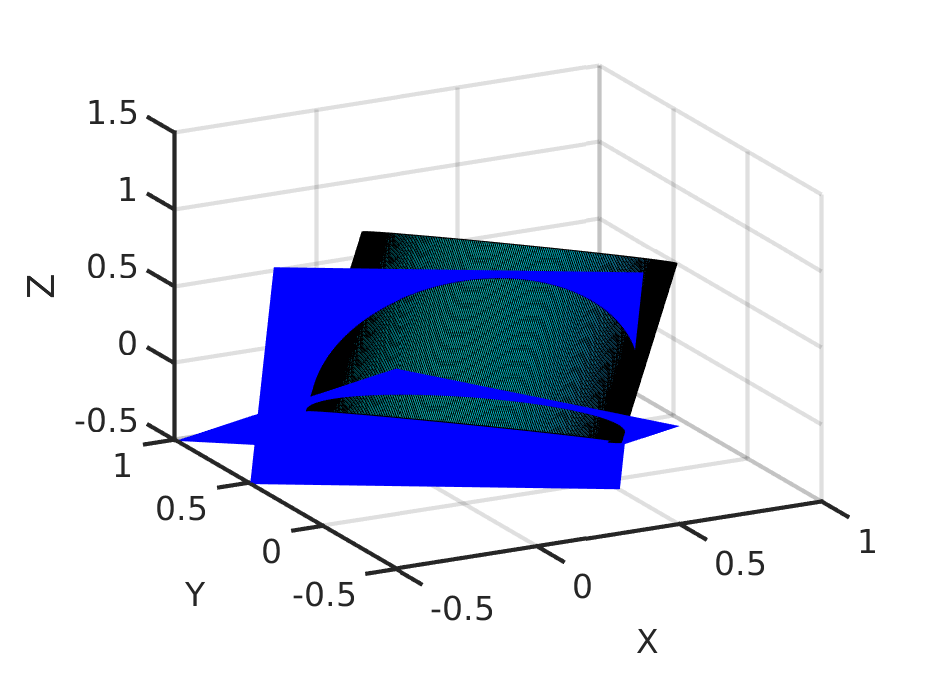
\includegraphics[width=.9\linewidth]{2hyper.eps}
		\caption{$m=2$}
	\end{subfigure}
	\begin{subfigure}[b]{0.25\textwidth}
		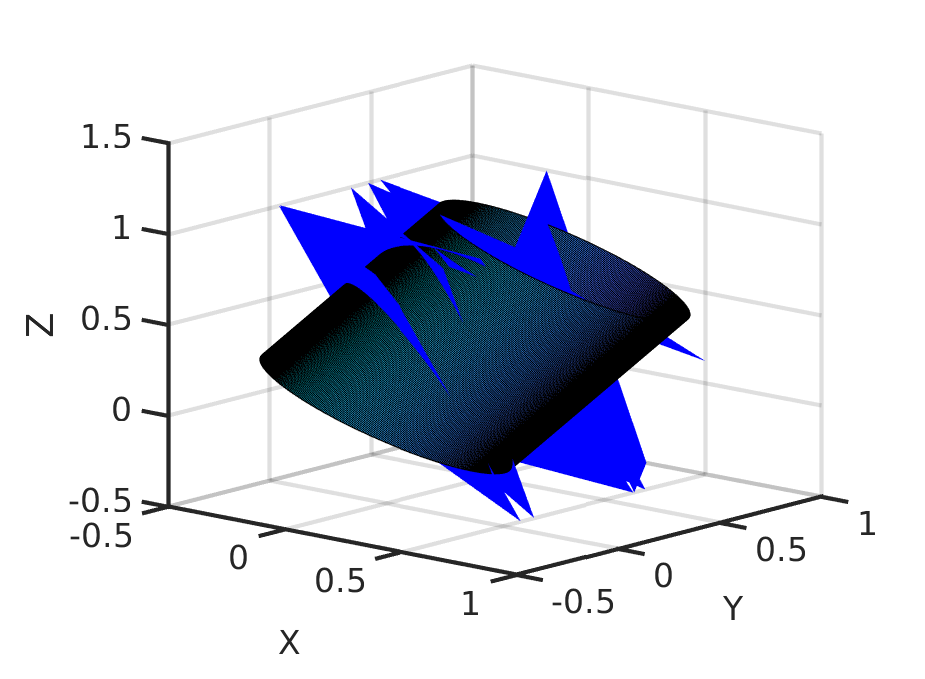
\includegraphics[width=.9\linewidth]{6hyper.eps}
		\caption{$m=6$}
	\end{subfigure}
	\begin{subfigure}[b]{0.25\textwidth}
		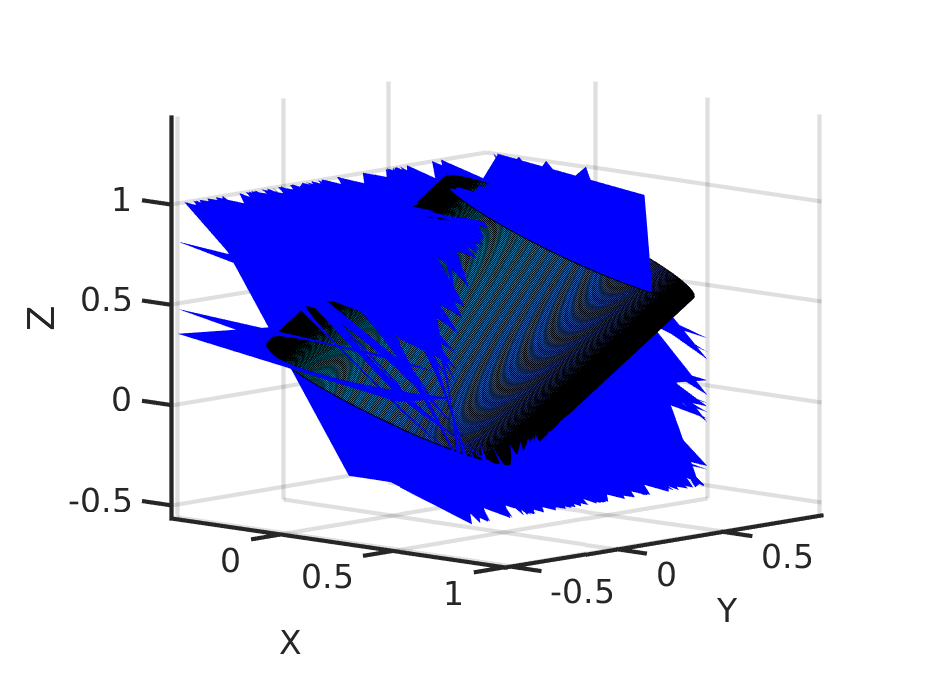
\includegraphics[width=.9\linewidth]{60hyper.eps}
		\caption{$m=60$}
	\end{subfigure}
		\begin{subfigure}[b]{0.25\textwidth}
		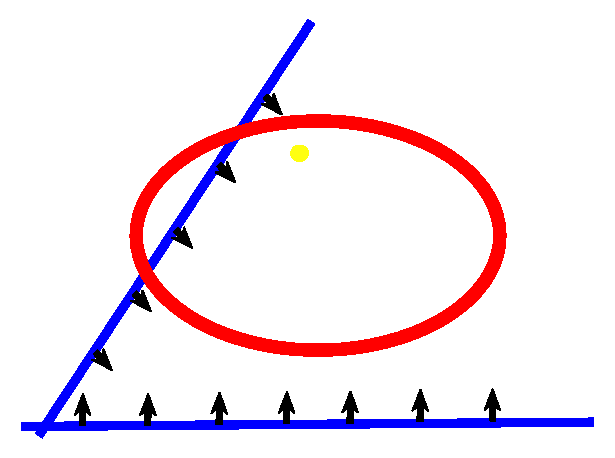
\includegraphics[width=.9\linewidth]{2D_2.eps}
		\caption{$m=2$}
	\end{subfigure}
		\begin{subfigure}[b]{0.25\textwidth}
		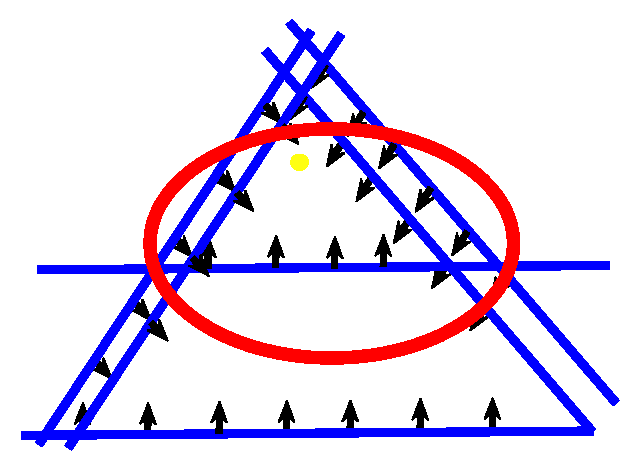
\includegraphics[width=.9\linewidth]{2D_6.eps}
		\caption{$m=6$}
	\end{subfigure}
		\begin{subfigure}[b]{0.25\textwidth}
		\includegraphics[width=.9\linewidth]{2D_60.eps}
		\caption{$m=60$}
	\end{subfigure}
\caption{Shrinkage of the one-bit polyhedron (\ref{eq:80n}) in blue, ultimately placed within the unit ball of the nuclear norm $\left\|\mbX\right\|_{\star}\leq 1$ shown with black cylindrical region and its red contours, when the number constraints (samples) grows large. The arrows point to the half-space associated with each inequality constraint. The evolution of the feasible regime is depicted with increasing samples in three cases: (a) and (d) small sample-size regime, constraints not forming a finite-value polyhedron; (b) and (e) medium sample-size regime, constraints forming a finite-volume polyhedron, parts of which are outside the cylinder; (c) and (f) large sample-size regime, constraints forming a finite-volume polyhedron inside the nuclear norm cylinder, making its constraint redundant. The optimal point representing the signal to be recovered is shown by yellow.}
\label{figure_1n}
\end{figure*}
\end{comment}
%\begin{comment}
\section{Judicious Sampling With Adaptive Thresholding for ORKA}
\label{ada_thresh}
%\textcolor{red}{move to last part (needs edits)}
By the spirit of using the iterative RKA, suitable time-varying sampling thresholds can be selected in order to enhance the recovery performance. In the sample abundance ORKA, we face a highly overdetermined linear feasibility problem creating a finite-volume space. To capture the desired signal $\mathbf{x}_{\star}$ more efficiently, the right-hand side of the inequalities in (\ref{eq:80n}), i.e. $\operatorname{vec}\left(\mbR\right)\odot \operatorname{vec}\left(\bGamma\right)$, must be determined in a way that each associated hyperplane passes through the desired feasible region within $\mathcal{F}_{\mbX}$. Therefore, an algorithm is proposed to ensure that this occurs in practice. Accordingly, we propose an iterative algorithm generating adaptive sampling thresholds to accurately obtain the desired solution. To have a smaller area of the finite-volume space around the desired signal $\mathbf{x}_{\star}$, one can somehow choose thresholds to reduce the distances between 
%them and 
the desired point and the associated hyperplanes in \eqref{eq:80n}. To do so, we update the time-varying thresholds 
%for $\ell\in\left\{1,\cdots,m\right\}$ 
as
\begin{equation}
\label{eq:200}
\left\{\begin{array}{l}
\boldsymbol{\uptau}^{(\ell)}_{k+1}=\mbA\mbx_{k}-\frac{1}{2}\left(\mbr^{(\ell)}\odot\boldsymbol{\epsilon}^{(\ell)}_{k}\right),\\\boldsymbol{\epsilon}^{(\ell)}_{k}=\mbr^{(\ell)}\odot\left(\mbA\mbx_k-\boldsymbol{\uptau}_{k}^{(\ell)}\right),
\end{array}\right.
\end{equation}\normalsize
where $\mbx_k$ and $\boldsymbol{\uptau}_{k}^{(\ell)}$ denote the $k$-th updates of $\mbx$ and $\boldsymbol{\uptau}^{(\ell)}$ in our proposed adaptive threshold design algorithm. 
%The discussion about the proper initialization of sampling thresholds in the adaptive threshold algorithm can be found in Supplementary Material.
%where $\bepsilon^{(\ell)}_{k}$ are positive vectors in the $k$-th iteration of the algorithm. This updating process is based on
%\begin{equation}
%\label{akhund}
%r_{j}=\begin{cases} +1 &\mba_{j}\mathbf{x}>\uptau_{j}, \\ -1&\mba_{j}\mathbf{x}<\uptau_{j},\end{cases}
%\end{equation}
%where $\{\mba_{j}\}$ are the rows of $\mbA$.
%The one-bit measurements $\left\{\mbr^{(\ell)}_{k}\right\}^{m}_{\ell=1}$ are updated in the way to satisfy (\ref{eq:80n}) in iteration $k$, i.e. the inequalities $\Omega^{(\ell)}_{k} \mbA\mathbf{x}_{\star}\geq \mbr^{(\ell)}_{k}\odot\boldsymbol{\uptau}^{(\ell)}_{k}$. The reason behind this updating is to ensure that each halfspace associated with a threshold in iteration $k$ is getting closer to the optimal point in the correct direction which means the main side of the halfspace is forced to cover the optimal solution. 
%Consider applying ORKA to a linear feasibility problem $\mbA\mathbf{x}= \mathbf{y}$ as part of the linear constraints of (\ref{eq:1nnnn}). Suppose the initial time-varying threshold sequences are $\left\{\boldsymbol{\uptau}^{(\ell)}_{0}\right\}\sim \mathcal{N}\left(0,1\right)$ (with the same length as $\mbr^{(\ell)}$), and $\left\{\delta^{(\ell)}\right\}$ are positive numbers. Also, $\mathbf{x}_{k}$, $\boldsymbol{\uptau}^{(\ell)}_{k}$, $\mbr^{(\ell)}_{k}$ and $\bepsilon_{k}$ denote their associated values at iteration $k$. 
The proposed sampling algorithm is summarized in Algorithm~\ref{algorithm_20}. By employing this adaptive thresholding algorithm, it is notable that each distance defined in \eqref{distance} tends to decrease, resulting in a reduction of $T_{\mathrm{ave}}$ with a high probability. Therefore, a smaller number of time-varying sampling threshold sequences can be utilized in ORKA with similar recovery performance. Additionally, non-informative sampling thresholds, which appear as extra inequality constraints in the random time-varying sampling thresholds scenario, may be efficiently removed by choosing the adaptive thresholds with closer hyperplanes to the desired point.
%\begin{enumerate}
  %  \item Find a point inside the following polyhedron with proposed accelerated Kaczmarz algorithms, i.e. the PrSKM or the block SKM for $\boldsymbol{\uptau}=\left\{\boldsymbol{\uptau}^{(\ell)}_{k}\right\}$:
   % $\mathcal{P}_{k}=\left\{\mathbf{x}_{k} \mid \Tilde{\bOmega}_{k}\mbA\mathbf{x}_{k}\succeq\mbb_{k}\right\},$ where $\mbb_{k}=\operatorname{vec}\left(\mbR_{k}\right)\odot \operatorname{vec}\left(\bGamma_{k}\right)$,  $\mbR_{k}$ and $\bGamma_{k}$ are matrices with $\left\{\mbr^{(\ell)}_{k}\right\}$ and $\left\{\boldsymbol{\uptau}^{(\ell)}_{k}\right\}$ representing their columns, respectively.
   % \item Update $\bGamma_{k+1}$ as:
 %  $\operatorname{vec}\left(\mbR_{k}\right)\odot \operatorname{vec}\left(\bGamma_{k+1}\right)=\Tilde{\bOmega}_{k}\mbA\mathbf{x}_{k}-\frac{\bepsilon_{k}}{2}$.
   
   % \item Compute $\bepsilon_{k}$, a block vector containing $\left\{\bepsilon^{(\ell)}_{k}\right\}$, as: $\bepsilon_{k}=\Tilde{\bOmega}_{k}\mbA\mathbf{x}_{k}-\operatorname{vec}\left(\mbR_{k}\right)\odot \operatorname{vec}\left(\bGamma_{k}\right).$    
    
    %\item Update $\mbR_{k+1}$ based on (\ref{akhund}):
%$ \mbr^{(\ell)}_{k+1}=\operatorname{sgn}\left(\mathbf{y}-\boldsymbol{\uptau}^{(\ell)}_{k+1}\right),\quad \ell \in \left\{1,\cdots,m\right\}$.
  %  \item Increase $k$ by one.
    %\item Stop when $\left\|\boldsymbol{\uptau}^{(\ell)}_{k+1}-\boldsymbol{\uptau}^{(\ell)}_{k}\right\|_{2}\leq \delta^{(\ell)}$.
%\end{enumerate}
\begin{algorithm}[t]
\caption{Adaptive Thresholding for ORKA}
\label{algorithm_20}
\begin{algorithmic}[1]
\Statex \emph{Input:} One-bit data,
%matrix $\mbR$, the 
time-varying sampling thresholds,
%matrix $\bGamma$, 
and the sampling matrix. %$\mbA\in\mathbb{R}^{n\times d}$. 
\Statex \emph{Output:} A solution $\bar{\mbx}$ in the one-bit polyhedron \eqref{eq:80n}.
%\State $k\gets 0$.
\State $\mbb^{(\ell)}\gets\boldsymbol{\uptau}_{k}^{(\ell)}$.
%\State $\mbb_{k}\gets \operatorname{vec}\left(\mbR_{k}\right)\odot \operatorname{vec}\left(\bGamma_{k}\right)$
\State $\mathcal{P}_{k}\gets\left\{\mathbf{x}_{k}\mid r_j^{(\ell)}\mba_j\mbx_k\geq r_j^{(\ell)}b_j^{(\ell)},~j\in[n],~\ell\in[m]\right\}$.
%$\mathcal{P}_{k}\gets\left\{\mathbf{x}_{k}\mid \Tilde{\bOmega}_{k}\mbA\mathbf{x}_{k}\succeq\mbb_{k}\right\}$
\State Obtain $\mbx_k$ in $\mathcal{P}_{k}$ by RKA, PrSKM or Block SKM.
%Find a point inside $\mathcal{P}_{k}$ with proposed accelerated Kaczmarz algorithms, i.e. the PrSKM or the Block SKM for $\boldsymbol{\uptau}=\left\{\boldsymbol{\uptau}^{(\ell)}_{k}\right\}$
\State $\boldsymbol{\epsilon}^{(\ell)}_{k}\gets\mbr^{(\ell)}\odot\left(\mbA\mbx_k-\mbb^{(\ell)}\right)$.
%Update $\bGamma_{k+1}$ as: $\operatorname{vec}\left(\mbR_{k}\right)\odot \operatorname{vec}\left(\bGamma_{k+1}\right)\gets\Tilde{\bOmega}_{k}\mbA\mathbf{x}_{k}-\frac{\bepsilon_{k}}{2}$.
\State $\boldsymbol{\uptau}^{(\ell)}_{k+1}\gets\mbA\mbx_{k}-\frac{1}{2}\left(\mbr^{(\ell)}\odot\boldsymbol{\epsilon}^{(\ell)}_{k}\right)$.
%Compute $\bepsilon_{k}$, a block vector containing $\left\{\bepsilon^{(\ell)}_{k}\right\}$, as: $\bepsilon_{k}\gets\Tilde{\bOmega}_{k}\mbA\mathbf{x}_{k}-\operatorname{vec}\left(\mbR_{k}\right)\odot \operatorname{vec}\left(\bGamma_{k}\right).$
%\State  Update $\mbR_{k+1}$ based on (\ref{akhund}):$ \mbr^{(\ell)}_{k+1}\gets\operatorname{sgn}\left(\mathbf{y}-\boldsymbol{\uptau}^{(\ell)}_{k+1}\right),\quad \ell \in \left\{1,\cdots,m\right\}$
\State Increase $k$ by one.
\State Repeat Steps ($1$)-($6$) until
%Stop when 
$\sum_{\ell=1}^{m}\left\|\boldsymbol{\uptau}^{(\ell)}_{k+1}-\boldsymbol{\uptau}^{(\ell)}_{k}\right\|_{2}\leq\delta$.
\State \Return $\bar{\mbx}$
\end{algorithmic}
\end{algorithm}
%One can observe that by deploying this adaptive thresholding algorithm, each distance defined in \eqref{distance}
%smaller values of $\{d_{j}\}$ will emerge which leads to their moments $\left\{\mu^{(\kappa)}_{d_{j}}\right\}$ to further diminish. Therefore, $\Psi_{T}$ is smaller in this scenario and a smaller number of time-varying sampling threshold sequences can be utilized in ORKA with similar recovery performance. Additionally, non-informative sampling thresholds, which appear as extra inequality constraints in the random time-varying sampling thresholds scenario, may be efficiently removed by choosing the adaptive thresholds with closer hyperplanes to the desired point.
%\end{comment}
\section{One-Bit Low-Rank Matrix Sensing}
\label{MATRIX}
Low-rank matrix sensing is an excellent example for problems that assume the form in (\ref{eq:1nnnn}), and that can be tackled using our methodology. In Section~\ref{pr}, we first briefly introduce the \emph{nuclear norm minimization} form of the low-rank matrix sensing problem. Subsequently, we apply ORKA to this problem without considering the associated costly constraints. 
%\Fr{Then in Section~\ref{matrixfactor}, we will present a new memory-efficient algorithm called \emph{ORKA with low-rank matrix factorization} suitable for large scale low-rank matrix sensing problems.} 
As mentioned previously, there exists a trade-off between the number of samples and the computational complexity of the reconstruction algorithm in the problem of signal parameters recovery. In 
%this 
Section~\ref{SVP}, we specifically address the scenario where, due to practical limitations or other factors, an adequate number of measurements or one-bit samples may not be available to satisfy the FVP described in Section~\ref{ada_thresh_prob}. To address this challenge, we will introduce a novel algorithm called \emph{SVP-ORKA}.
%new variants of the RKA algorithm.


\subsection{Problem Formulation}
\label{pr}
The problem of the low-rank matrix sensing is formulated as:
\begin{equation}
\label{eq:1nnnnn}
\begin{aligned}
\text{find}\quad \mbX \in \Omega_{c} \quad
\text{subject to} \quad \mathcal{A}\left(\mbX\right)=\mathbf{y},~ 
\operatorname{rank}\left(\mbX\right)\leq r,
\end{aligned}
\end{equation}\normalsize
where $\mbX\in \mathbb{R}^{n_{1}\times n_{2}}$ is the matrix of unknowns, $\mathbf{y}\in \mathbb{R}^{n}$ is the measurement vector, and $\mathcal{A}$ is a linear transformation such that $\mathcal{A}:\mathbb{R}^{n_1\times n_2}\mapsto\mathbb{R^{n}}$.
%$n_{1}\times n_{2}$ into $\mathbb{R}^{n}$. 
In general, $\Omega_{c}$ can be chosen such as the set of semi-definite matrices, symmetric matrices, upper or lower triangle matrices, Hessenberg matrices and a specific constraint on the matrix elements $\left\|\mbX\right\|_{\infty}\leq \alpha$ or on its eigenvalues, i.e., $\lambda_{i}\leq \epsilon$ where $\left\{\lambda_{i}\right\}$ are eigenvalues of $\mbX$ \cite{davenport2016overview,candes2015phase,van1996matrix}. The problem (\ref{eq:1nnnnn}) can be rewritten as an optimization problem:
\begin{equation}
\label{eq:1nnnnnn}
\begin{aligned}
\underset{\mbX \in \Omega_{c}}{\textrm{minimize}}\quad \operatorname{rank}\left(\mbX\right) \quad
\text{subject to} \quad \mathcal{A}\left(\mbX\right)=\mathbf{y}.
\end{aligned}
\end{equation}\normalsize
This problem is known to be NP-hard, whose solution is difficult to approximate \cite{meka2008rank,recht2011null}. Recall that the rank of $\mbX$ is equal to the number of nonzero singular values. In the
case when the singular values are all equal to one, the sum of the singular values is equal to the rank. When the singular values are less than or equal to one, the sum of the singular values is a convex function that is strictly less than the rank. Therefore, it has been popular for this problem to replace the rank function with
the sum of the singular values of $\mbX$; i.e., its nuclear norm. The nuclear norm minimization alternative of the problem is given by \cite{cai2010singular,recht2010guaranteed,recht2011null}:
\begin{equation}
\label{eq:1nnnnnnn}
\begin{aligned}
\underset{\mbX \in \Omega_{c}}{\textrm{minimize}}\quad \left\|\mbX\right\|_{\star}\quad
\text{subject to} \quad \mathcal{A}\left(\mbX\right)=\mathbf{y}.
\end{aligned}
\end{equation}
In this problem, the feasible set $\mathcal{F}_{\mbX}$ is obtained as
$\mathcal{F}_{\mbX}=\left\{\mathcal{P}^{\star}_{\mbX}\cap \Omega_{c}\right\}$,
where $\mathcal{P}^{\star}_{\mbX}$ is defined as follows
\begin{equation}
\label{stephanie}
\mathcal{P}^{\star}_{\mbX} = \left\{\mbX \mid
\left\|\mbX\right\|_{\star}\leq \tau\right\},\quad
\tau\in\mathbb{R}^{+}.
\end{equation}\normalsize
Next, we will apply ORKA to (\ref{eq:1nnnnnnn}) to make its costly constraints redundant by using abundant number of one-bit samples $m^{\prime}$.
%time-varying sampling thresholds $m$. 

In low-rank matrix sensing, the linear operator $\mathcal{A}\left(\mbX\right)$ is obtained as \cite{chi2019nonconvex},
\begin{equation}
\label{Stefanie_2}
\mathcal{A}\left(\mbX\right)=\frac{1}{\sqrt{n}}\left[\operatorname{Tr}\left(\mbA^{\top}_1\mbX\right)\cdots\operatorname{Tr}\left(\mbA^{\top}_n\mbX\right)\right]^{\top},
\end{equation}
where $\mbA_j\in\mathbb{R}^{n_1\times n_2}$ is the $j$-th sensing matrix. The one-bit polyhedron for the low-rank matrix sensing is given by
\begin{equation}
\label{kumar}
\mathcal{P}^{(M)}=\left\{\mbX \mid r^{(\ell)}_{j}\operatorname{Tr}\left(\mbA^{\top}_j\mbX\right)\geq r^{(\ell)}_{j}\tau^{(\ell)}_{j},~j\in[n],~\ell\in[m]\right\}.  
\end{equation}
Writing the update process of ORKA in matrix form yields the following representation:
\begin{equation}
\label{Stefanie_1}   
\mbX_{i+1} =\mbX_i+\frac{\left(r^{(\ell)}_j\tau^{(\ell)}_j-r^{(\ell)}_j\operatorname{Tr}\left(\mbA^{\top}_j\mbX_i\right) \right)^{+}}{\left\|\mbA_{j}\right\|^{2}_{\mathrm{F}}} \mbA_{j}.
\end{equation}
By applying the vectorization operator to both sides of \eqref{Stefanie_1} and utilizing the fact that $\left\|\mbA_j\right\|_{\mathrm{F}}=\left\|\operatorname{vec}\left(\mbA_j\right)\right\|_2$, we obtain an update process identical to that of RKA. Therefore, the convergence rate of this process is equivalent to that of RKA. Denote the update process in \eqref{Stefanie_1} by $\mbX_{i+1}=\mathrm{KA}_{r}(\mbX_i)$.
One can similarly utilize other variants of RKA, PrSKM and Block SKM, and generalize the update process \eqref{Stefanie_1} as $\mbX_{i+1}=\mathrm{KA}_{p}(\mbX_i)$ and $\mbX_{i+1}=\mathrm{KA}_{b}(\mbX_i)$.

A numerical investigation of (\ref{kumar}) 
%when it is achieved for the nuclear norm minimization, 
reveals that by increasing the number of time-varying sampling threshold sequences $m$, the space formed by the intersection of half-spaces (inequality constraints) can fully shrink to the desired signal $\mbX_{\star}$ inside the feasible region of (\ref{stephanie}) which is shown by the cylindrical space \cite{recht2011null}---see Fig.~\ref{figure_1n} for an illustrative example of this phenomenon. As can be seen in this figure, the blue lines displaying the linear feasibility form a finite-volume space around the original signal displayed by the yellow circle inside the cylinder (the elliptical region) by growing the number of threshold sequences or one-bit samples. In (a)/(d), constraints are not enough to create a finite-volume space, whereas in (b)/(e) such constraints can create the desired finite-volume polyhedron space which, however, is not fully inside the cylinder. Lastly, in (c)/(f), the created finite-volume space shrinks to be fully inside the cylinder. The theoretical discussion regarding the required number of one-bit samples $m^{\prime}$ to accurately recover the low-rank matrix from the polyhedron \eqref{kumar} has been presented in Section~\ref{penalt}.
%\Fr{Denote $\bar{\mbX}$ as the recovered low-rank matrix by ORKA in the sample abundance scenario. In the following corollary, we present the minimum number of one-bit samples $m^{\prime}$ such that $\bar{\mbX}\in\mathcal{B}_{r}(\mbX_{\star})$:
%\begin{corollary}
%\label{low_rank_orka}
%\end{corollary}
%}
\begin{comment}
\begin{figure*}[t]
	\centering
	\begin{subfigure}[b]{0.35\textwidth}
		\includegraphics[width=1\linewidth]{rank-one-nmse.eps}
		\caption{}
	\end{subfigure}
	\begin{subfigure}[b]{0.35\textwidth}
		\includegraphics[width=1\linewidth]{rank-four-nmse.eps}
		\caption{}
	\end{subfigure}
	\caption{Average NMSE for the Frobenius norm of error for the recovery of the matrix $\mbX$ associated with different time-varying sampling threshold sequences sizes when the PrSKM and the block SKM are utilized in ORKA: (a) $\operatorname{rank}\left(\mbX\right)=1$, (b) $\operatorname{rank}\left(\mbX\right)=4$.}
	\label{figure_2}
\end{figure*}
\begin{figure*}[t]
	\centering
	\begin{subfigure}[b]{0.35\textwidth}
		\includegraphics[width=1\linewidth]{rank-one-nmse-adaptive-threshold.eps}
		\caption{}
	\end{subfigure}
	\begin{subfigure}[b]{0.35\textwidth}
		\includegraphics[width=1\linewidth]{rank-four-nmse-adaptive-threshold.eps}
		\caption{}
	\end{subfigure}
	\caption{Comparing the average NMSE for the Frobenius norm of error for the recovery of the matrix $\mbX$ using ORKA when (i) a random threshold and (ii) the adaptive sampling threshold are adopted when the block SKM is utilized in ORKA: (a) $\operatorname{rank}\left(\mbX\right)=1$, (b) $\operatorname{rank}\left(\mbX\right)=4$.}
	\label{figure_3}
\end{figure*}
\end{comment}
%---------------------------------------------------------------
\begin{figure}[t]
	\centering
	\subfloat[$m=2$]
		{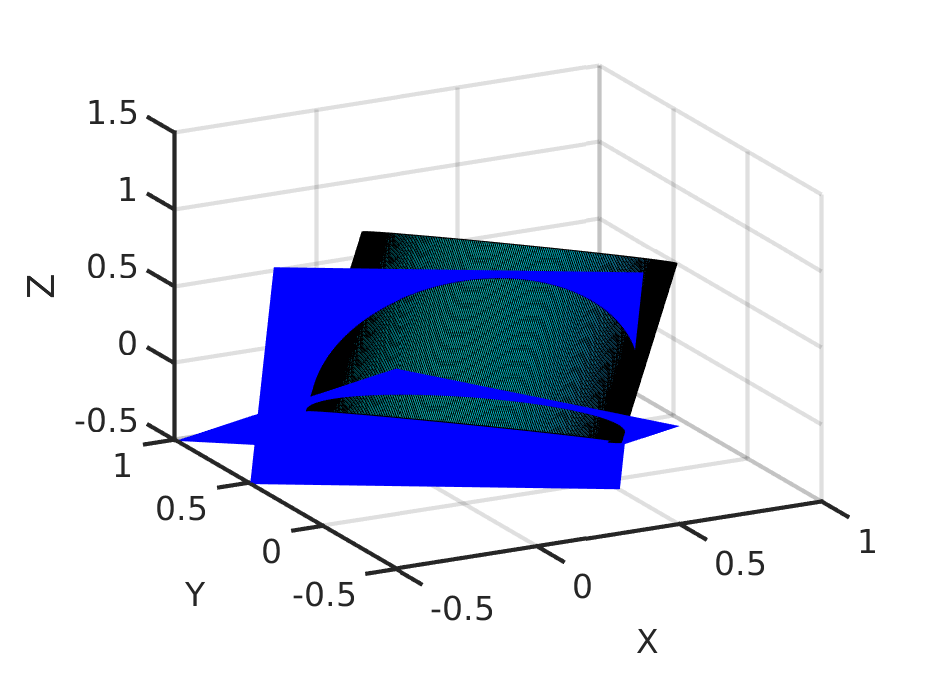
\includegraphics[width=0.25\textwidth]{2hyper.eps}}
	\subfloat[$m=6$]
		{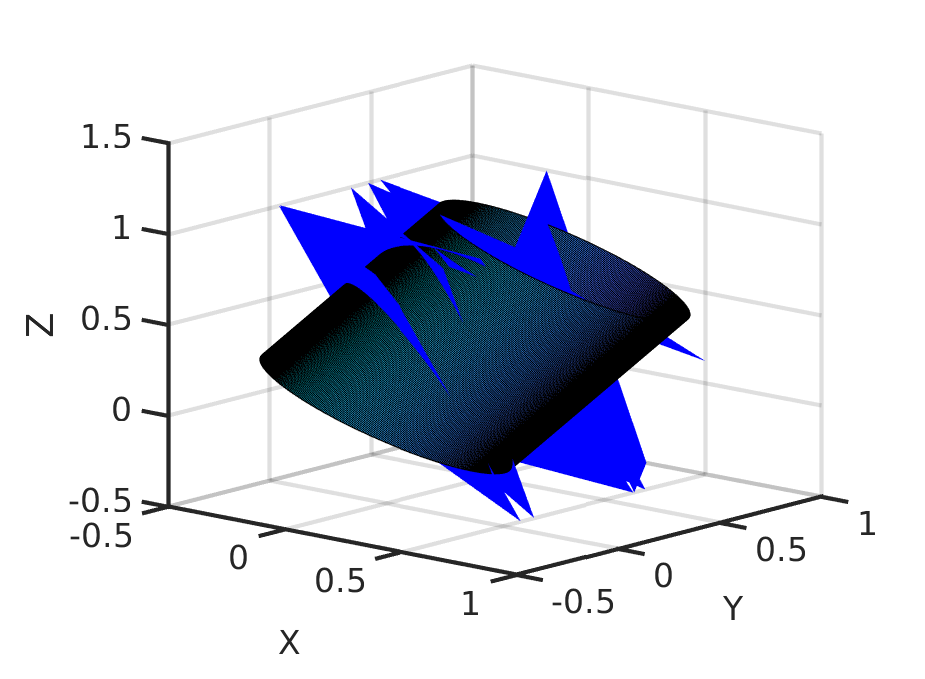
\includegraphics[width=0.25\textwidth]{6hyper.eps}}
	\subfloat[$m=60$]
		{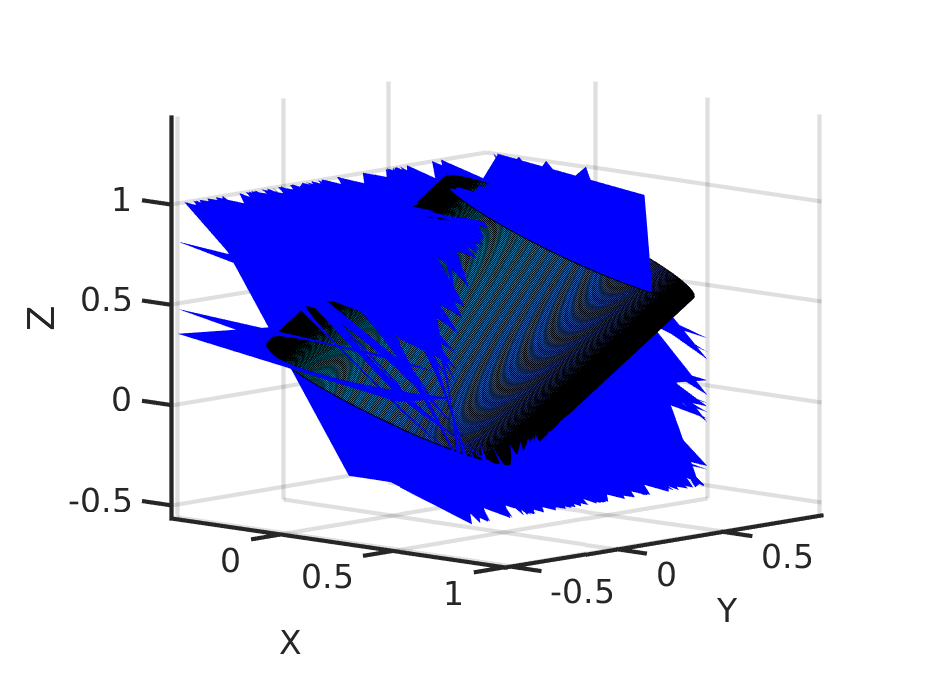
\includegraphics[width=0.25\textwidth]{60hyper.eps}}\\
	\subfloat[$m=2$]
		{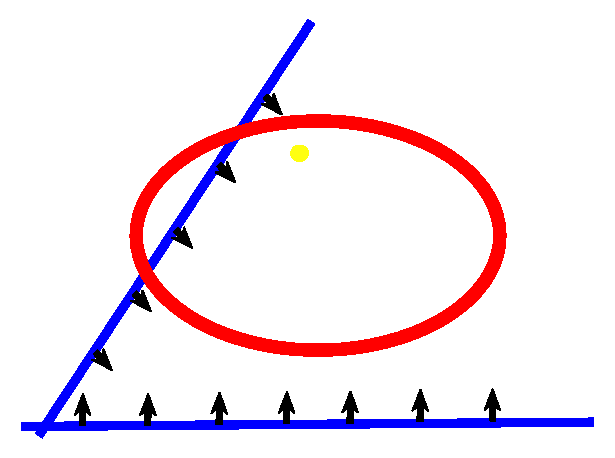
\includegraphics[width=0.25\textwidth]{2D_2.eps}}
	\subfloat[$m=6$]
		{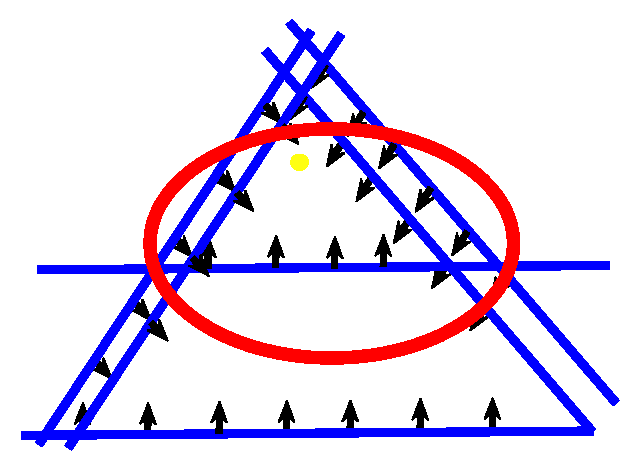
\includegraphics[width=0.25\textwidth]{2D_6.eps}}
	\subfloat[$m=60$]
		{\includegraphics[width=0.25\textwidth]
        {2D_60.eps}}
	\caption{Shrinkage of the one-bit polyhedron (\ref{eq:80n}) in blue, ultimately placed within the unit ball of the nuclear norm $\left\|\mbX\right\|_{\star}\leq 1$ shown with black cylindrical region and its red contours, when the number constraints (samples) grows large. The arrows point to the half-space associated with each inequality constraint. The evolution of the feasible regime is depicted with increasing samples in three cases: (a) and (d) small sample-size regime, constraints not forming a finite-value polyhedron; (b) and (e) medium sample-size regime, constraints forming a finite-volume polyhedron, parts of which are outside the cylinder; (c) and (f) large sample-size regime, constraints forming a finite-volume polyhedron inside the nuclear norm cylinder, making its constraint redundant. The original signal representing the signal to be recovered is shown by yellow.
    \vspace{-15pt}
	}
	\label{figure_1n}
\end{figure}
%-----------------------------------------------------------------
\subsection{ORKA With Low-Rank Matrix Factorization}
\label{matrixfactor}
Although Kaczmarz algorithms use a simple and low-complexity update process, the computational cost can still be prohibitively large for a matrix $\mbX\in\mathbb{R}^{n_1\times n_2}$ when $n_1$ and $n_2$ are large values, typically requiring $\mathcal{O}\left(n_1 n_2\right)$ operations. To address this issue, we employ the well-known \emph{low-rank matrix factorization} technique. Instead of using the full matrix $\mbX$, we use its low-rank factorization $\mbX=\mbL\mbW^{\top}$, where $\mbL\in\mathbb{R}^{n_1\times r}$ and $\mbW\in\mathbb{R}^{n_2\times r}$ are low-rank factors. The advantage of this approach is that the economical representation of the low-rank matrix results in lower storage requirements, lower per-iteration computational cost, and better amenability to parallelization. It also makes the method more scalable to larger problem sizes, especially when using iterative optimization methods like ORKA. %There is a rich discussion regarding the combining the low-rank matrix factorization with gradient descent methods \cite{chi2019nonconvex}. 
The combination of low-rank matrix factorization with gradient descent methods has been extensively discussed in the literature \cite{chi2019nonconvex}. In this section, we explore the integration of low-rank matrix factorization with ORKA and the alternating minimization (AltMin) algorithm discussed in \cite{jain2010guaranteed}. 

%The one-bot polyhedron $\mathcal{P}^{(M)}$ with low-rank minimization is written as
The one-bit polyhedron $\mathcal{P}^{(M)}$ associated with the low-rank matrix factorization approach is written as
\begin{equation}
\label{kvm_15}
\mathcal{P}^{(M)}_0=\left\{\mbL, \mbW \mid r^{(\ell)}_{j}\operatorname{Tr}\left(\mbA^{\top}_j\mbL\mbW^{\top}\right)\geq r^{(\ell)}_{j}\tau^{(\ell)}_{j},~j\in[n],~\ell\in [m]\right\}.
\end{equation}
To find the solution from $\mathcal{P}^{(M)}_0$, we use the idea of AltMin algorithm. We split $\mathcal{P}^{(M)}_0$ into two linear feasibility sub-problems with respect to $\mbL$ and $\mbW$, respectively. Specifically, with respect to $\mbL$ when $\mbW$ is fixed we have:
\begin{equation}
\label{kvm_16}
\mathcal{P}^{(M)}_{\mbL}=\left\{\mbL\mid r^{(\ell)}_{j}\operatorname{Tr}\left(\mbW^{\top}\mbA^{\top}_j\mbL\right)\geq r^{(\ell)}_{j}\tau^{(\ell)}_{j},~j\in[n],~\ell\in [m]\right\},
\end{equation}
and with respect to $\mbW$ when $\mbL$ is fixed we have:

\begin{equation}
\label{kvm_17}
\mathcal{P}^{(M)}_{\mbW}=\left\{\mbW \mid r^{(\ell)}_{j}\operatorname{Tr}\left(\mbA^{\top}_j\mbL\mbW^{\top}\right)\geq r^{(\ell)}_{j}\tau^{(\ell)}_{j},~j\in[n],~\ell\in [m]\right\}.
\end{equation}\normalsize
If either $\mbL$ or $\mbW$ are fixed, finding the solution with respect to the other variable is achieved via ORKA as indicated in Algorithm~\ref{algorithm_200}.
%\begin{enumerate}
   % \item For $t=0,\cdots, T$ do:
   % \item To update $\mbW$, solve the inequality $r^{(\ell)}_{j}\operatorname{Tr}\left(\mbA_j\mbL^{(t)}\mbW^{\top}\right)\geq r^{(\ell)}_{j}\uptau^{(\ell)}_{j}$ and set the obtained solution as $\mbW^{(t+1)}$.
   % \item Compute the solution for $\mbL$ that satisfies $r^{(\ell)}_{j}\operatorname{Tr}\left(\mbW^{(t+1)\top}\mbA_j\mbL\right)\geq r^{(\ell)}_{j}\uptau^{(\ell)}_{j}$, and denote this solution as $\mbL^{(t+1)}$.
   % \item Once the algorithm has converged, denote the obtained solutions as $\mbL_{\star}=\mbL^{(T)}$ and $\mbW_{\star}=\mbW^{(T)}$.
   % \item $\mbX_{\star}=\mbL_{\star}\mbW^{\top}_{\star}$.
%\end{enumerate}
\begin{algorithm}[t]
\caption{ORKA (with Low-Rank Matrix Factorization)}
\label{algorithm_200}
\begin{algorithmic}[1]
\Statex \emph{Input:} One-bit samples, 
%$\left\{r^{(\ell)}_{j}\right\}^{m^{\prime}}_{j,\ell=1}$, 
time-varying thresholds and
%$\left\{\uptau^{(\ell)}_{j}\right\}^{m^{\prime}}_{j,\ell=1}$, 
the sensing %sampling 
matrices presented in \eqref{kvm_15},
%$\left\{\mbA_j\in\mathbb{R}^{n_1\times n_2}\right\}^{n}_{j=1}$, 
total number of required iterations $T$, and $\operatorname{rank}(\mbX_{\star})=r$.
\Statex \emph{Output:} A solution $\bar{\mbX}\in\mathbb{R}^{n_1\times n_2}$ in the polyhedron \eqref{kvm_15}.
%one-bit low-rank matrix sensing feasible set $\mathcal{P}^{(M)}_0$.
\Statex \emph{Note:} $\mbL_t\in\mathbb{R}^{n_1\times r}$ and $\mbW_t\in\mathbb{R}^{n_2\times r}$ denote the obtained matrices at $t$-th iteration, $\mbH_{i+1}=\mathrm{KA}_{r}(\mbH_{i};\Tilde{\mbH})$ denotes the update process of ORKA using the RKA when $\Tilde{\mbH}$ is fixed.
%\State $\mbX\gets \mbL\mbW^{\top}$ $\triangleright$ $\mbL\in\mathbb{R}^{n_1\times r}$ and $\mbW\in\mathbb{R}^{n_2\times r}$.
%\State $\triangleright$ $\mbW^{(t)}$ and $\mbL^{(t)}$ the obtained matrices at $t$-th iteration. 
\State $\mbW_{t+1}\gets\mathrm{KA}_{r}(\mbW_t;\mbL_t)$ $\triangleright$ Update process for polyhedron \eqref{kvm_17}.
%To update $\mbW$, solve the inequality $r^{(\ell)}_{j}\operatorname{Tr}\left(\mbA^{\top}_j\mbL^{(t)}\mbW^{\top}\right)\geq r^{(\ell)}_{j}\uptau^{(\ell)}_{j}$ and set the obtained solution as $\mbW^{(t+1)}$.
\State $\mbL_{t+1}\gets\mathrm{KA}_{r}(\mbL_t;\mbW_{t+1})$ $\triangleright$ Update process for polyhedron \eqref{kvm_16}.
%Compute the solution for $\mbL$ that satisfies $r^{(\ell)}_{j}\operatorname{Tr}\left(\mbW^{(t+1)\top}\mbA^{\top}_j\mbL\right)\geq r^{(\ell)}_{j}\uptau^{(\ell)}_{j}$, and denote this solution as $\mbL^{(t+1)}$.
\State Repeat steps (1) and (2) until convergence. %and obtain $\mbX_{\star}$.
\State %Once the algorithm has converged, denote the obtained solutions as 
$\mbL_{\star}\gets\mbL_T$ and $\mbW_{\star}\gets\mbW_T$.
\State \Return  $\bar{\mbX}\gets\mbL_{\star}\mbW^{\top}_{\star}$.
\end{algorithmic}
\end{algorithm}

\subsection{Curse of Dimensionality: SVP-ORKA}
\label{SVP}
While acquiring a large number of samples is not typically an issue for one-bit sampling, it is still practical to avoid using excess samples, particularly in signal processing applications where access to sufficient measurements may be limited. Adhering to the law of parsimony, ``\emph{Entia non svnt mvltiplicanda præter necessitatem}," i.e., entities should not be multiplied beyond necessity, this section focuses on developing ORKA to facilitate low-rank matrix sensing with a reduced number of one-bit samples. As with any technique, there is a trade-off between the number of samples and the complexity of that technique, and this section aims to address the challenges associated with a limited number of samples.

Define $r$ 
%and $R$ 
as the predefined rank 
%and the bound on the Frobenius norm 
of the unknown matrix $\mbX$.
%, respectively. 
In order to obtain the solution within a reduced number of samples in the polyhedron $\mathcal{P}^{(M)}$ defined in \eqref{kumar}, we impose 
%(i) 
a rank constraint, $\operatorname{rank}(\mbX)\leq r$,
%, and (ii) the Frobenius norm constraint, $\|\mbX\|_{\mathrm{F}}\leq R$,
to shrink the entire space, as shown by the following polyhedron:
\begin{equation}
\label{Stefanie_5}
\mathcal{P}^{(M)}_1=\left\{\mbX \mid r^{(\ell)}_{j}\operatorname{Tr}\left(\mbA^{\top}_j\mbX\right)\geq r^{(\ell)}_{j}\tau^{(\ell)}_{j},~ \operatorname{rank}\left(\mbX\right)\leq r\right\},
\end{equation}\normalsize
%where $r$ is the predefined rank of unknown matrix $\mbX$ and 
where $j\in[n],~\ell \in [m]$. To tackle this problem, we apply the SVP method to ORKA. The SVP was introduced as a solution to the general affine rank minimization problem (ARMP). In \cite{jain2010guaranteed}, it was demonstrated that the SVP can effectively recover the minimum rank solution even in the presence of noise and when the affine constraints satisfy RIP. Moreover, some theoretical guarantees for this approach were also established. This method utilizes the operator
$P_{r}$ %operator 
to modify the gradient descent process at each iteration. The operator $P_{r}$ 
%operator 
calculates the $r$ largest singular values of a matrix and subsequently rewrites its SVD based on these $r$ singular values and their corresponding singular vectors. Similar to Section~\ref{pr}, denote $\mathrm{KA}_r(\cdot)$ as the update process of ORKA using the RKA defined in \eqref{Stefanie_1}. Through the integration of SVP into each iteration of ORKA, we can achieve the following update process:
\begin{equation}
\label{St_20}
\left\{\begin{array}{l}
\mbZ_{i+1}=\mathrm{KA}_{r}(\mbX_i),\\
%\mbX_i+\frac{\left(r^{(\ell)}_j\uptau^{(\ell)}_j-r^{(\ell)}_j\operatorname{Tr}\left(\mbA^{\top}_j\mbX_i\right) \right)^{+}}{\left\|\mbA_{j}\right\|^{2}_{\mathrm{F}}} \mbA_{j}\\
\mbX_{i+1}=P_{r}\left(\mbZ_{i+1}\right).
\end{array}\right.
\end{equation}\normalsize
The first step of the update process \eqref{St_20}, $\mbZ_{i+1}=\mathrm{KA}_{r}(\mbX_i)$, can be also replaced with $\mbZ_{i+1}=\mathrm{KA}_{p}(\mbX_i)$ or $\mbZ_{i+1}=\mathrm{KA}_{b}(\mbX_i)$ to be consistent with the updates of PrSKM and Block SKM, respectively. The convergence guarantee of SVP-ORKA is concluded according to the following lemma:
\begin{lemma}
\label{Ea}
The update process of SVP-ORKA presented in \eqref{St_20} converges linearly in expectation to a ball centered at the original signal
%$\bar{\mbX}\in \mathcal{B}_{\rho}\left(\mbX_{\star}\right)$
$\mathcal{B}_{\rho}\left(\operatorname{vec}\left(\mbX_{\star}\right)\right)$ 
with the number of samples satisfying Theorem~\ref{TH10-Stephania❤️} and probability exceeding $1-\eta$, as follows:
%The convergence of SVP-ORKA for solving the linear feasibility problem $\mathcal{P}^{(M)}_1$ is expressed as follows:
\begin{equation}
\label{kvm_19}
\begin{aligned}
\mathbb{E}\left\{\left\|\mbX_{i+1}-\mbX_{\star}\right\|^2_{\mathrm{F}}\right\}\leq\left(1-\frac{1}{\kappa^{2}\left(\mbV\right)}\right)^{i} \left\|\mbX_{0}-\widehat{\mbX}\right\|^2_{\mathrm{F}}+\rho^2,
\end{aligned}   
\end{equation}\normalsize
where $\widehat{\mbX}\in \mathcal{P}^{(M)}_{1}$,
%$\widehat{\mbX}\in \mathcal{P}^{(M)}_{1}\left(\operatorname{vec}\left(\mbX_{\star}\right)\right)$, 
and $\mbV$ is the matrix with vectorized sensing matrices $\left\{\operatorname{vec}\left(\mbA_j\right)\right\}^{n}_{j=1}$ as its rows. 
\end{lemma}
The proof of Lemma~\eqref{Ea} is studied in Appendix~\ref{svp_proof}.
%Section H-(2) of the Supplementary Material. 
%$\Tilde{\mbX}_{i+1}=f_{R}(\mbX_{i+1})$ within the update process of \eqref{St_20}, we ensure that the constraint $\|\mbX\|_{\mathrm{F}}\leq R$ is satisfied in each iteration.
%guarantees that the constraint $\|\mbX\|_{\mathrm{F}}\leq R$ satisfies in each iteration.
%In addition to Theorem~\ref{TH10-Stephania❤️}, which provides the required number of one-bit samples for achieving perfect one-bit low-rank matrix sensing, we also present the development of random hyperplane tessellations specifically for low-rank matrix sensing with dithered one-bit quantization. This novel extension of the random hyperplane tessellations framework is comprehensively detailed in \cite, offering valuable insights into the application of this technique in the context of dithered one-bit quantization for low-rank matrix sensing.

\begin{comment}
\begin{figure*}[t]
	\centering
	\begin{subfigure}[b]{0.35\textwidth}
		\includegraphics[width=1\linewidth]{CS1.eps}
		\caption{}
	\end{subfigure}
	\begin{subfigure}[b]{0.35\textwidth}
		\includegraphics[width=1\linewidth]{CS2.eps}
		\caption{}
	\end{subfigure}
	\caption{Average NMSE for the error between the desired signal $\mathbf{x}_{\star}$ and its recovered version $\bar{\mathbf{x}}$ for different time-varying sampling threshold sequences sizes when the PrSKM and the block SKM are utilized in ORKA with (a) $k=2$, (b) $k=4$.}
	\label{figure_4}
\end{figure*}
\end{comment}

\section{One-Bit Compressed Sensing:\\ 
From Optimization to Linear Feasibility}
CS is an interesting and rapidly growing area of research that has attracted considerable attention in electrical engineering, applied mathematics, statistics, and computer science \cite{eldar2012compressed,davenport2016overview}. In CS, 
%a sparse high-dimensional signal is to be recovered from incomplete measurements with such a recovery that may be formulated as
the objective is to recover a sparse high-dimensional signal from incomplete measurements, which may be formulated as follows \cite{eldar2012compressed}:
\begin{equation}
\label{eq:1nnnnnnnm}
\begin{aligned}
\underset{\mbx}{\textrm{minimize}}\quad \left\|\mathbf{x}\right\|_{1}\quad
\text{subject to}\quad \mbA\mathbf{x}=\mathbf{y},
\end{aligned}
\end{equation}
where $\mbA\in\mathbb{R}^{n\times d}$, and $n\ll d$. 
%One of the important applications of CS emerges in the signal recovery from a sequence of acquisitions $\{y_{i}\}$ obtained from a sparse linear transformation (wavelet transformations are known for such a property, for instance) in the magnetic resonance imaging (MRI). The reconstruction problem of the desired signal $\mathbf{x}^{\star}$ is given by
%\begin{equation}
%\label{eq:1nnnnnnnmm}
%\begin{aligned}
%\min_{\mathbf{x}}\quad & \left\|\mathbf{x}\right\|_{1}\\
%\text{s.t.} \quad &\mathcal{A}_{i}\left(\mathbf{x}\right)=y_{i},\quad i\in\left\{1,\cdots,n\right\}.
%\end{aligned}
%\end{equation}
%In this section, we first formulate the optimization problem of the \emph{one-bit compressed sensing}. Then, by taking advantage of one-bit sampling, we increase sample size in (\ref{eq:1nnnnnnnmm}) and create an  associated one-bit polyhedron.

The concise summary of CS theory mentioned earlier implies that, under ideal circumstances, the measurement vector $\mby$ is assumed to be represented with infinite precision. However, real-world sensing models typically involve digitalization and finite precision data representations for purposes such as storing, transmitting, or processing acquired observations.

%The one-bit Compressed Sensing (one-bit CS) problem has been the subject of extensive research, with many approaches proposed to solve it, in particular, the binary iterative hard thresholding (BIHT) and its normalized version, normalized BIHT (NBIHT) 

%As a result, we are inspired to 
Following our motivation in one-bit low-rank matrix recovery, herein we are inspired to investigate the one-bit CS problem in (i) sample abundance, and (ii) sample restricted scenarios. In Section~\ref{ocs_abundance}, our goal is to 
%we are inspired to investigate how one-bit quantization with multiple time-varying threshold sequences affects CS, and to 
examine the reconstruction performance of one-bit CS with multiple time-varying threshold sequences under a sample-abundance regime without any form of regularization. Beyond the sample abundance scenario, in Section~\ref{ocs_constrained} we also develop the ORKA for conditions where enough measurements to create a highly-overdetermined feasibility problem are not available. It is crucial to highlight that the choice of a particular one-bit 
%sampling 
reconstruction scheme for compressed sensing measurements is heavily influenced by factors such as available computational resources, implementation complexity, and cost considerations associated with the sensor. %Each scheme presents distinct trade-offs in terms of computational power and resource requirements, allowing users to select the most suitable option based on their unique needs and constraints.

\subsection{One-Bit CS via Sample Abundance}
\label{ocs_abundance}
%Denote $\mba_j$ as the $j$-th row of the sampling matrix $\mbA$. Similar to Section~\ref{one-bit}, the one-bit samples associated with the feasibility $\mby=\mbA\mbx$ are generated as
%Let $\boldsymbol{\uptau}$ denotes the time-varying threshold vector. The one-bit samples are generated as
%\begin{equation}
%\label{eq:101}
%\begin{aligned}
%r_{j} &= \begin{cases} +1 & \mba_{j}\mathbf{x}\geq\tau^{(\ell)}_{j}, \\ -1 & \mba_{j}\mathbf{x}<\tau^{(\ell)}_{j}.
%\end{cases}
%\end{aligned}
%\end{equation}
%where $\mathcal{A}_{i}\left(\mathbf{x}\right)=\mba^{\top}_{i}\mathbf{x}$.
\begin{comment}
The occurrence probability vector $\mbp$ for the one-bit measurement $\mbr$ is given as \cite{eamaz2022phase},
\begin{equation}
\label{eq:102}
\begin{aligned}
p_{i} &= \begin{cases} \Phi\left(\mba^{\top}_{i}\mathbf{x}\right) & \text{for}\quad \{r_{i}=+1\}, \\ 1-\Phi\left(\mba^{\top}_{i}\mathbf{x}\right) &\text{for}\quad \{r_{i}=-1\},
\end{cases}
\end{aligned}
\end{equation}
where $\Phi(.)$ is the CDF of $\boldsymbol{\uptau}$. The log-likelihood function of the sign data $\mbr$ is given by
\begin{equation}
\label{eq:103}
\begin{aligned}
\mathcal{L}_{\mbr}(\bmu,\mathbf{x}) &= \sum^{m}_{i=1}\left\{\mathbb{I}_{(r_{i}=+1)}\log\left(\Phi(\mba^{\top}_{i}\mathbf{x})\right) \right.\\& \left.+\mathbb{I}_{(r_{i}=-1)}\log\left(1-\Phi(\mba^{\top}_{i}\mathbf{x})\right)\right\}.
\end{aligned}
\end{equation}
Therefore, the maximum likelihood estimation (MLE) for the one-bit compressed sensing can be written as
\begin{equation}
\label{one-cs}
\min_{\mathbf{x}} \mathcal{L}_{\mbr}(\bmu,\mathbf{x})+\lambda \|\mathbf{x}\|_{1}.
\end{equation}
The alternative formulations for one-bit compressed sensing can be found in \cite{khobahi2020model}.
\end{comment}
As discussed earlier, by deploying one-bit quantization, the opportunity exists to increase the number of samples in (\ref{eq:1nnnnnnnm}). The one-bit CS is thus solely accomplished by creating a highly-constrained one-bit polyhedron:
\begin{equation}
\label{Stefanie_500}
\mathcal{P}^{(C)}=\left\{\mbx\mid r^{(\ell)}_{j}\mba_j\mbx\geq r^{(\ell)}_{j}\tau^{(\ell)}_{j},~ j\in[n],~\ell\in[d]\right\}.
\end{equation}
In other words, instead of solving an optimization problem with costly constraints, the problem may be tackled by 
%the proposed accelerated Kaczmarz algorithms; namely, PrSKM and the Block SKM such as 
the following update process:
\begin{equation}
\label{kvm_23}
\mbx_{i+1}=\mathrm{KA}_{r}\left(\mbx_i\right),
%\mbx_i+\frac{\left(r^{(\ell)}_j\uptau^{(\ell)}_j-r^{(\ell)}_j\mba_j\mbx_i\right)^{+}}{\left\|\mba_{j}\right\|^{2}_2} \mba^{\mathrm{H}}_j.
\end{equation}
where $\mathrm{KA}_r(\cdot)$ denotes the RKA update process presented as $\mbx_{i+1}=\mbx_i+\frac{\left(r^{(\ell)}_j\tau^{(\ell)}_j-r^{(\ell)}_j\mba_j\mbx_i\right)^{+}}{\left\|\mba_{j}\right\|^{2}_2} \mba^{\mathrm{H}}_j$. The update process in \eqref{kvm_23} can be also replaced with $\mbx_{i+1}=\mathrm{KA}_{p}\left(\mbx_i\right)$ or $\mbx_{i+1}=\mathrm{KA}_{b}\left(\mbx_i\right)$ to be consistent with the updates of PrSKM and Block SKM, respectively. The theoretical discussion about the minimum number of one-bit samples $m^{\prime}$ to precisely recover the sparse vector from the polyhedron \eqref{Stefanie_500} has been presented in Section~\ref{penalt}.

\begin{comment}
\begin{figure*}[t]
	\centering
	\begin{subfigure}[b]{0.35\textwidth}
		\includegraphics[width=1\linewidth]{CS3.eps}
		\caption{}
	\end{subfigure}
	\begin{subfigure}[b]{0.35\textwidth}
		\includegraphics[width=1\linewidth]{CS4.eps}
		\caption{}
	\end{subfigure}
	\caption{Comparing the average NMSE for the desired signal $\mathbf{x}_{\star}$ and its recovered signal using ORKA when (i) a random threshold and (ii) the adaptive sampling threshold are adopted with (a) $k=20$, (b) $k=40$}
	\label{figure_5}
\end{figure*}
\end{comment}

\subsection{ Regularized ORKA for One-Bit CS: ST-ORKA}
\label{ocs_constrained}
In this section, we continue our exploration of algorithms for one-bit CS by introducing the \emph{$\ell_1$ regularized ORKA}. Building on the motivation behind our earlier proposal of the SVP-ORKA, ORKA is developed to efficiently recover
%identify 
a sparse solution from the one-bit CS polyhedron using a reduced number of one-bit samples. This feature proves particularly useful in scenarios where the number of measurements is severely limited. The regularized one-bit CS polyhedron is obtained as
\begin{equation}
\label{Stefanie_50}
\mathcal{P}^{(C)}_1=\left\{\mbx\mid r^{(\ell)}_{j}\mba_j\mbx\geq r^{(\ell)}_{j}\tau^{(\ell)}_{j},~ \left\|\mbx\right\|_1\leq \upkappa\right\},
\end{equation}
where $j\in[n]$ and $\ell\in[m]$.
%In the polyhedron \eqref{Stefanie_50}, assume $\|\mbx\|_0\leq s$. To see the connection between the value of $\upkappa$ and $s$, without loss of generality assume $\|\mbx\|_2\leq 1$ in the polyhedron \eqref{Stefanie_50}. Then, based on the relation $\|\mbx\|_1\leq\sqrt{\|\mbx\|_0}\|\mbx\|_2\leq\sqrt{s}$, we have $\upkappa=\sqrt{s}$. 
Define the soft thresholding (ST) operator as $S_{\upkappa}\left(\mbx\right)= \operatorname{sgn}\left(\mbx\right)\left(|\mbx|-\mbt_1\right)^{+}$, where $\mbt_1$ is the predefined threshold. The ST-ORKA utilizes the %soft thresholding 
ST operator $S_{\upkappa}$ 
%operator 
to project each iteration of ORKA to the set $\left\{\|\mbx\|_1\leq\upkappa\right\}$
%convex hull of $\ell_1$. 
%The ST operator is defined as $S_{\upkappa}\left(\mbx\right)= \operatorname{sgn}\left(\mbx\right)\left(|\mbx|-\mbt_1\right)^{+}$, where $\mbt_1$ is the predefined threshold. 
%Therefore, the ST-ORKA algorithm is given by 
with the following update process:
\begin{equation}
\label{St_21}
\left\{\begin{array}{l}
\mbz_{i+1}=\mathrm{KA}_r\left(\mbx_i\right),\\
%\mbx_i+\frac{\left(r^{(\ell)}_j\uptau^{(\ell)}_j-r^{(\ell)}_j\mba_j\mbx_i\right)^{+}}{\left\|\mba_{j}\right\|^{2}_2} \mba^{\mathrm{H}}_j\\
\mbx_{i+1} = S_{\upkappa}\left(\mbz_{i+1}\right),
\end{array}\right.
\end{equation}
where $\mathrm{KA}_r(\cdot)$ denotes the RKA updates. The first step of the update process \eqref{St_21} can be also replaced with $\mbz_{i+1}=\mathrm{KA}_p\left(\mbx_i\right)$ or $\mbz_{i+1}=\mathrm{KA}_b\left(\mbx_i\right)$ to be consistent with the updates of PrSKM and Block SKM, respectively. The convergence rate of ST-ORKA is studied in the following lemma:
\begin{lemma}
\label{kvm_24}
Consider a ball centered at the original signal $\mathcal{B}_{\rho}\left(\mbx_{\star}\right)$ and $\widehat{\mbx}\in\mathcal{P}^{(C)}_{1}$, the convergence of ST-ORKA presented in \eqref{St_21} is given by
\begin{equation}
\label{kvm_25}
\begin{aligned}
\mathbb{E}\left\{\left\|\mbx_{i+1}-\mbx_{\star}\right\|^2\right\}\leq\left(1-\frac{1}{\kappa^{2}\left(\mbA\right)}\right)^{i} \left\|\mbx_{0}-\widehat{\mbx}\right\|^2_2+\rho^2,
\end{aligned}
\end{equation}\normalsize
with a probability exceeding
$1-\eta$, and the number of samples satisfying Theorem~\ref{TH10-Stephania}.
\end{lemma}
The proof of Lemma~\ref{kvm_24} is studied in Appendix~\ref{sta}.
%Section H-(1) of the Supplementary Material. 
Note that to have a guaranteed convergence, one can integrate ORKA with different operators that satisfy Lipschitz continuity. This is important in various applications and provides a chance to go beyond just ST-ORKA and SVP-ORKA.
%We can use different operators that satisfy Lipschitz continuity to update the ORKA process for various applications, beyond just ST-ORKA and SVP-ORKA. 
By doing so, we can achieve a convergence rate that is described in the following lemma: 
\begin{lemma}
\label{Ea1}
Assume $f(\cdot)$ is an operator such that for any $\mbx_1,\mbx_2\in\mathbb{R}^{d}$ we have
$\left\|f\left(\mbx_1\right)-f\left(\mbx_2\right)\right\|_2^2 \leq L \left\|\mbx_1-\mbx_2\right\|_2^2$.
Then the integration of RKA with the operator $f$ in each iteration of solving the feasibility problem $\mbC\mbx\succeq\mbb$ with $\mbC\in\mathbb{R}^{n\times d}$ has the following convergence rate:
\begin{equation}
\mathbb{E}\left\{\left\|\mbx_{i+1}-\widehat{\mbx}\right\|^2_2\right\}\leq L\left(1-\frac{1}{\kappa^{2}\left(\mbC\right)}\right)^{i} \left\|\mbx_{0}-\widehat{\mbx}\right\|^2_2.
\end{equation}\normalsize
\begin{comment}
The convergence of the projected RKA algorithm for solving a linear feasibility problem $\mbC\mbx\succeq \mbb$ involves the application of a Lipschitz continuous projector function $f(\cdot)$ at each iteration. The convergence rate can be expressed as follows:
\begin{equation}
\begin{aligned}
\mathbb{E}\left\{\left\|\mbx_{i+1}-\mbx_{\star}\right\|^2_2\right\}\leq L\left(1-\frac{1}{\kappa^{2}\left(\mbC\right)}\right)^{i} \left\|\mbx_{0}-\mbx_{\star}\right\|^2_2,
\end{aligned}
\end{equation}
where $f(\cdot)$ satisfies the condition:
\begin{equation}
\label{Lip}
\left\|f\left(\mbx_1\right)-f\left(\mbx_2\right)\right\|_2 \leq L \left\|\mbx_1-\mbx_2\right\|_2.
\end{equation}
\end{comment}
\end{lemma}
A notable example for Lemma~\ref{Ea1} is the integration of ORKA with the hard thresholding (HT) operator $\mathcal{T}_s(\cdot)$ to reconstruct the $s$-sparse signal in the one-bit CS problem.
%An alternative option for the operator used in ORKA to reconstruct the $s$-sparse signal is the application of \emph{hard thresholding} (HT), represented by $\mathcal{T}_s(\cdot)$. 
This operator selects the best $s$-sparse approximation of the solution at each iteration. The algorithm is named HT-ORKA with the update process presented as
\begin{equation}
\label{kvm_30}
\left\{\begin{array}{l}
\mbz_{i+1}=\mathrm{KA}_r\left(\mbx_i\right),\\
%\mbx_i+\frac{\left(r^{(\ell)}_j\uptau^{(\ell)}_j-r^{(\ell)}_j\mba_j\mbx_i\right)^{+}}{\left\|\mba_{j}\right\|^{2}_2} \mba^{\mathrm{H}}_j\\
\mbx_{i+1} = \mathcal{T}_s\left(\mbz_{i+1}\right).
\end{array}\right.
\end{equation}
The convergence rate of HT-ORKA can be determined using the following lemma:
\begin{lemma}
\label{ht_orka}
Assume $\mathcal{B}_{\rho}\left(\mbx_{\star}\right)$ be a ball centered at the original signal and $\widehat{\mbx}\in\mathcal{P}^{(C)}_{1}$, the convergence of HT-ORKA presented in \eqref{kvm_30} is given by
%, can be expressed as follows:
\begin{equation}
\begin{aligned}
\mathbb{E}\left\{\left\|\mbx_{i+1}-\mbx_{\star}\right\|^2\right\}\leq 2\left(1-\frac{1}{\kappa^{2}\left(\mbA\right)}\right)^{i} \left\|\mbx_{0}-\widehat{\mbx}\right\|^2_2+\rho^2. 
\end{aligned}
\end{equation}\normalsize
with probability higher than
$1-\eta$, and the number of samples satisfying Theorem~\ref{TH10-Stephania}.
\end{lemma}
The proof of Lemma~\ref{ht_orka} is provided in Appendix~\ref{htt_orka}.
%Section H-(3) of the Supplementary Material. %It is important to note that the set $\mathcal{H}_{d,s}$ defined in \eqref{kvm_69} is the convex hull of the set $\bar{\mathcal{H}}_{d,s}=\left\{\mbx\in\mathbb{R}^{d}\mid\|\mbx\|_0\leq s,\|\mbx\|_2\leq 1\right\}$. Therefore, the guarantees discussed earlier remain valid for HT-ORKA as well.
In their work, the authors of \cite{plan2014dimension} introduced the random hyperplane tessellations theorem for the ditherless scenario in one-bit CS, specifically targeting the reconstruction of signal direction. This theorem was developed in \cite{baraniuk2017exponential} for one-bit CS with Gaussian dithering,
%In our study, we propose the FVP to determine the required number of one-bit samples. 
%Furthermore, 
where based on the augmentation trick \cite{baraniuk2017exponential,foucart2019recovering}, random hyperplane tessellations are limited to Gaussian random variables for the sampling matrix and normal distribution for the dithering.
%as stated in \cite{baraniuk2017exponential}. 
The random hyperplane tessellations theorem has previously been %developed 
extended for certain non-Gaussian sampling matrices in \cite{dirksen2022sharp,dirksen2021non}. In their work, the authors derived theoretical guarantees for Uniform dithering and focused on the Hamming distance.
The main distinction between the FVP and random hyperplane tessellations lies in the modeling of the created finite volume around the original signal. While random hyperplane tessellations utilize Hamming distance to capture the direction of measurements, we incorporate Euclidean distance between the one-bit hyperplanes and the original signal, considering the importance of amplitude in dithered one-bit sensing. 
By using the Euclidean distances between the original signal and the surrounding hyperplanes as the basis of our work, we were able to obtain theoretical guarantees beyond Uniform dithering. This is a crucial distinction, as it highlights the significance of the difference between measurements and thresholds in one-bit sensing. Intuitively, if measurements and thresholds become closer and closer, the recovery performance improves.
%Additionally, the FVP does not impose any norm restrictions, which exist in the random hyperplane tessellations framework.

\section{Numerical Investigations}
In this section, we conduct numerical evaluations to assess the performance of our proposed algorithms in two distinct scenarios: (i) sample abundance and (ii) sample restriction. All presented results are averaged over 1000 experiments.

\subsection{Sample abundance}
In this particular scenario, we examine two examples: one-bit low-rank matrix sensing and one-bit CS. For both cases, we employ the Block SKM algorithm to recover the desired signal and then evaluate its performance against the adaptive threshold strategy introduced in \cite[Section~\rom{6}]{eamaz2022phase}. The only distinction is that, in this study, we did not update the one-bit data to account for an exceedingly low-complexity hardware implementation.
%and compare its performance with the adaptive threshold strategy presented in \cite[Section~\rom{6}]{eamaz2022phase} with the only difference that here we did not update the one-bit data to take into account a very low-complexity hardware implementation.
%Section~\ref{ada_thresh}. 
In all experiments, we have taken into account the presence of Gaussian additive noise, also known as \emph{prequantization error}, with a standard deviation of $0.1$.
\\
\textbf{One-bit low-rank matrix sensing.} We considered a set of sampling matrices $\{\mbA_j\}_{j=1}^{1800}$, where each entry is independently drawn from a standard normal distribution. We have generated the desired matrix $\mbX_{\star}\in\mathbb{R}^{30\times 30}$ such that $\operatorname{rank}(\mbX_{\star})=2$. The number of time-varying sampling threshold sequences were set to $m\in\{1,10,20,30\}$. Accordingly, we have generated sequences of time-varying sampling thresholds as $\left\{\boldsymbol{\uptau}^{(\ell)}\sim \mathcal{N}\left(\mathbf{0},\frac{\beta_{\mby}^2}{9}\mathbf{I}\right)\right\}_{\ell=1}^{m}$, where $\beta_{\mby}$ denotes the dynamic range of the high-resolution measurements $\mby$. Figure \ref{figure_2}(a) illustrates a comparison between the recovery performance of Block SKM using random thresholds and %Block SKM using 
adaptive thresholds. It is evident that the utilization of adaptive thresholds enhances the recovery performance compared to random thresholds.
\\
\textbf{One-bit CS.} We have generated a sensing matrix $\mbA\in\mathbb{R}^{500\times 100}$ in which each element follows a standard normal distribution. The desired signal $\mbx_{\star}\in\mathbb{R}^{100}$ was assumed to have the level of sparsity $s=10$. The settings for time-varying sampling thresholds were considered to be the same as the one-bit low-rank matrix sensing case. Fig.~\ref{figure_2}(b) displays the recovery performance of Block SKM using random thresholds in comparison with adaptive thresholds. Consistent with previous observations, the utilization of adaptive thresholds improves the recovery performance.
%-------------------------------------------------------
\begin{figure}[t]
	\centering
	\subfloat[]
		{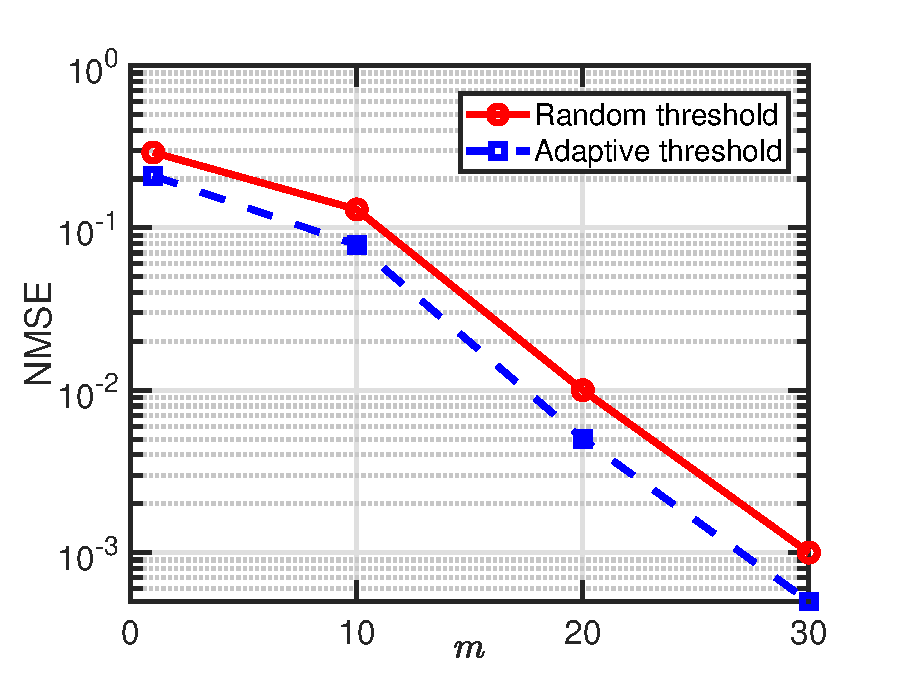
\includegraphics[width=0.47\columnwidth]{matrix-sensing-abundance.eps}}
    \subfloat[]
		{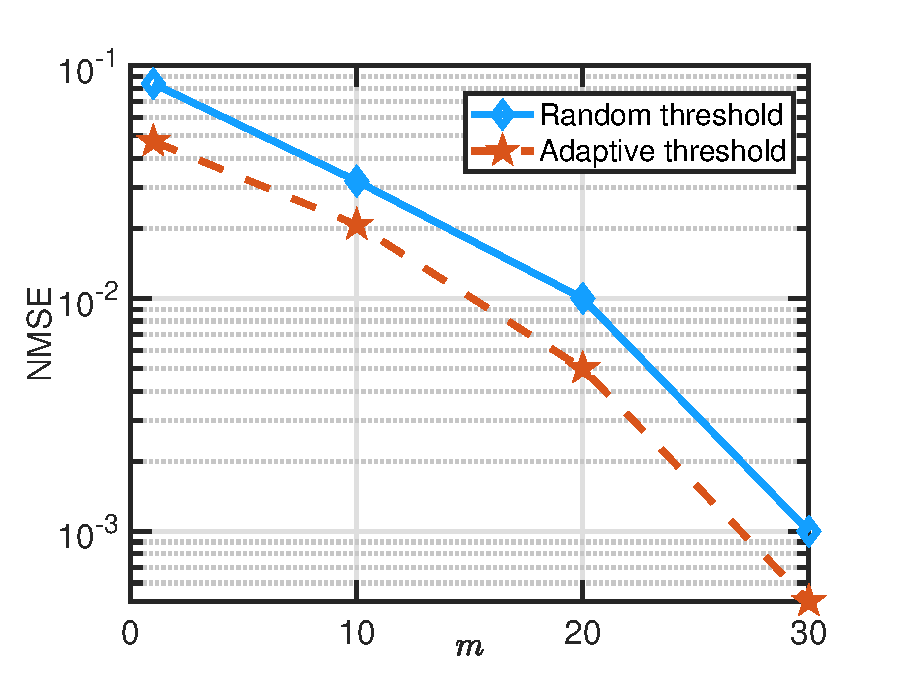
\includegraphics[width=0.47\columnwidth]{cs-abundance.eps}}
	\caption{Comparison between the recovery performance of Block SKM using random thresholds and adaptive thresholds in the sample abundance scenario for (a) one-bit low-rank matrix sensing, and (ii) one-bit CS.
  \vspace{-15pt}
 }
	\label{figure_2}
\end{figure}
%-------------------------------------------------------
\subsection{Sample Scarcity}
Similar to sample abundance, herein we investigate the performance of our proposed methods for one-bit low-rank matrix sensing and one-bit CS when we have a limited number of samples. Note that in all experiments, the high-resolution measurements were contaminated by the additive Gaussian noise with the standard deviation $0.1$ except the case related to low-rank matrix sensing by SVP-ORKA which was considered to be noiseless.
\\
\textbf{One-bit low-rank matrix sensing.} We generated a collection of sampling matrices $\{\mbA_j\}_{j=1}^{n}$, where each entry is independently sampled from a standard normal distribution. The desired matrix $\mbX_{\star}\in\mathbb{R}^{30\times 30}$ was generated with $\operatorname{rank}(\mbX_{\star})=2$. Define the oversampling factor as $\lambda=\frac{n}{n_1r}=\frac{n}{60}$. In our experiments, we have set 
%the oversampling factor to 
$\log(\lambda)\in\{3,4,5,6\}$. The number of time-varying sampling threshold sequences was fixed at $m=1$. The generation of time-varying sampling thresholds followed the same procedure as in the previous cases. Fig.~\ref{figure_3}(a) compares the recovery performance of SVP-ORKA with hard singular value thresholding (HSVT) algorithm \cite{foucart2019recovering} in the noiseless scenario. As can be observed, SVP-ORKA outperforms HSVT over different values of the oversampling factor. In another experimental setting aimed at assessing the performance of Algorithm~\ref{algorithm_200} (ORKA with low-rank matrix factorization), we generated the desired matrix $\mbX_{\star}\in\mathbb{R}^{30\times 30}$ with $\operatorname{rank}(\mbX_{\star})=1$. The remaining parameter settings were identical to the previous example. Note that in this case we define the oversampling factor as $\beta=\frac{n}{n_1^2r}=\frac{n}{900}$. In our simulations, we have set $\beta=\{5,10,15,20\}$. As can be seen in Fig.~\ref{figure_3}(b), the recovery performance of Algorithm~\ref{algorithm_200} enhances as the value of the oversampling factor $\beta$ grows large.
%-------------------------------------------------------
\begin{figure}[t]
	\centering
	\subfloat[]
		{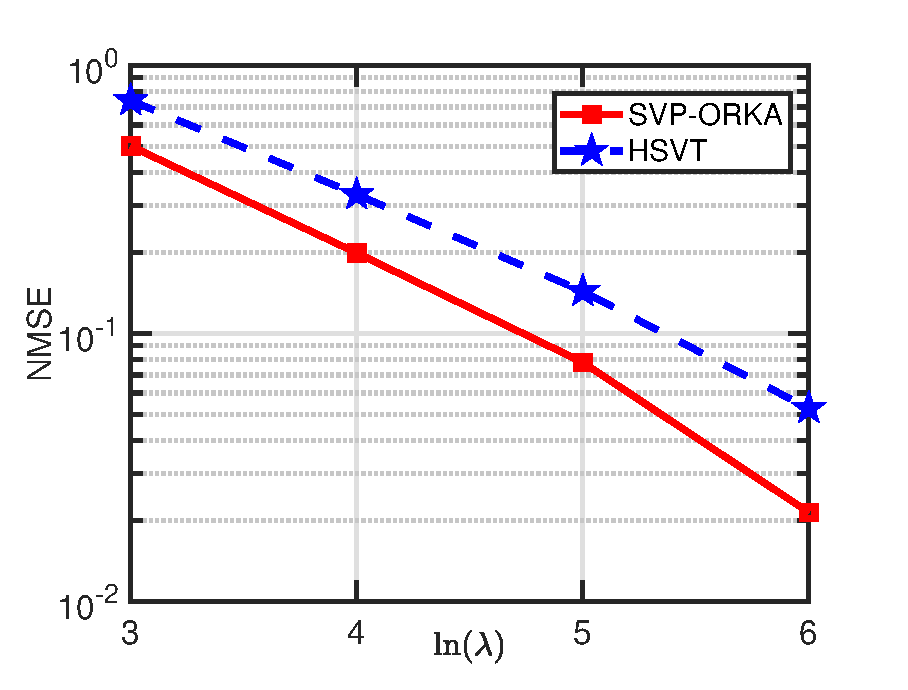
\includegraphics[width=0.47\columnwidth]{matrix-sensing-constraint.eps}}
    \subfloat[]
		{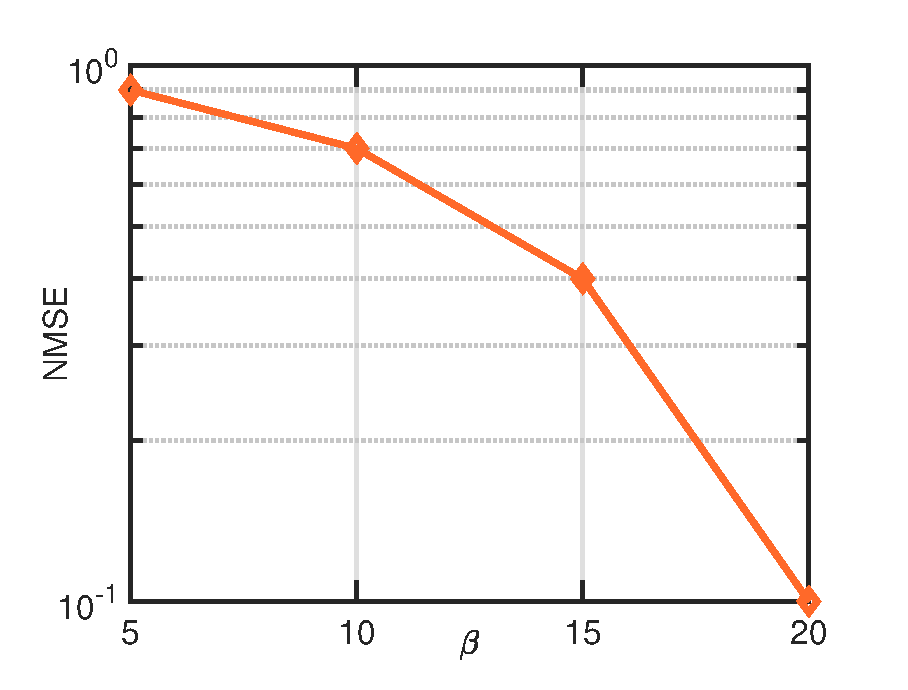
\includegraphics[width=0.47\columnwidth]{factorization.eps}}
	\caption{(a) Comparison between the recovery performance of SVP-ORKA and HSVT algorithm over different values of oversampling factor $\lambda$. (b) Recovery performance of Algorithm~\ref{algorithm_200} (ORKA with low-rank matrix factorization) over different values of sampling factor $\beta$.
  \vspace{-15pt}
 }
	\label{figure_3}
\end{figure}
%-------------------------------------------------------
%-------------------------------------------------------
\begin{figure}[t]
	\centering
	\subfloat[]
		{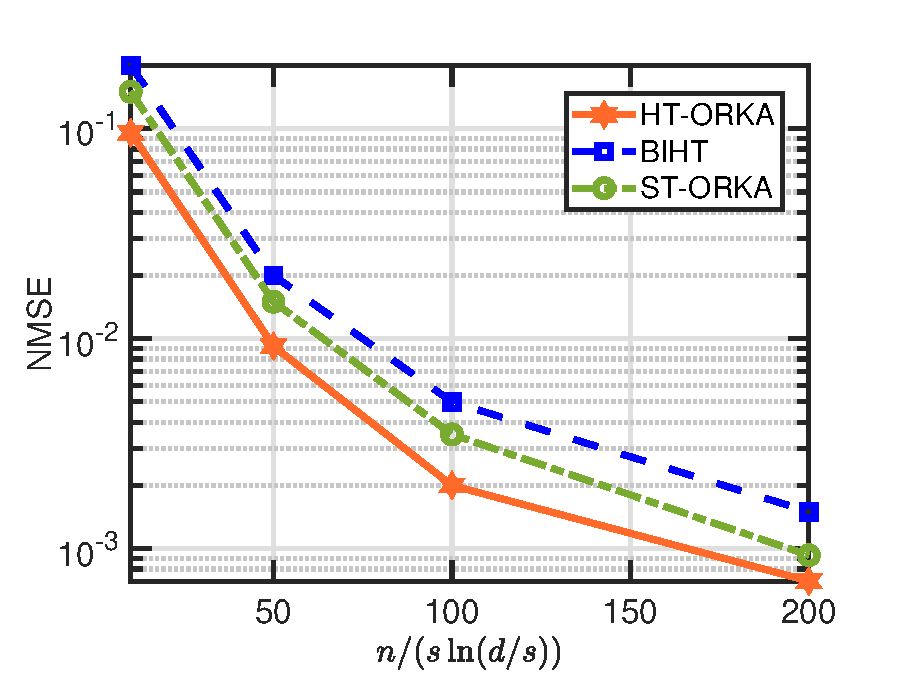
\includegraphics[width=0.47\columnwidth]{cs-constraint-threshold.eps}}
    \subfloat[]
		{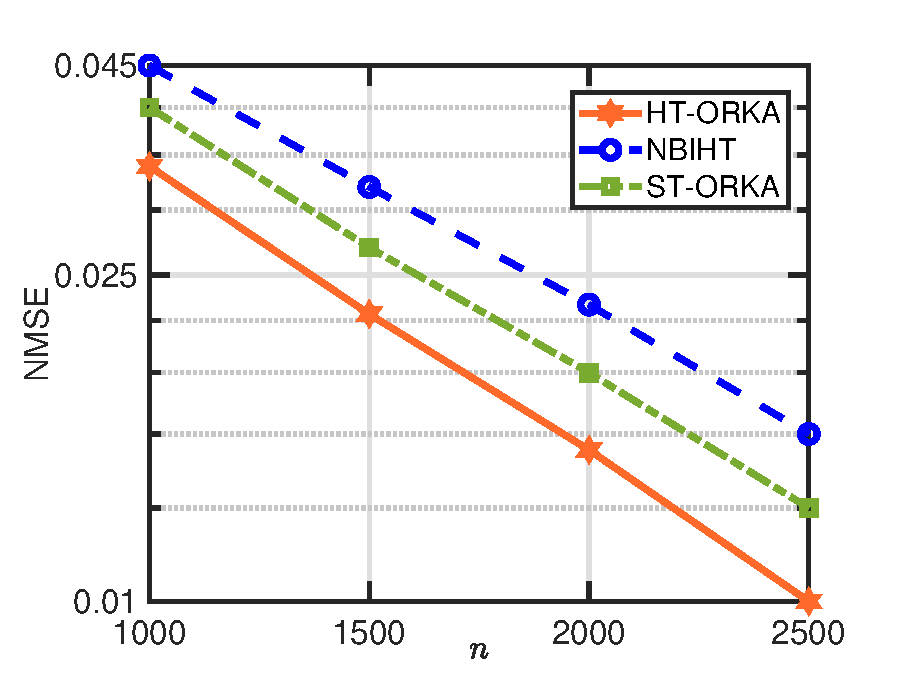
\includegraphics[width=0.47\columnwidth]{cs-constraint-zero.eps}}
	\caption{Comparison between the recovery performance of HT-ORKA, ST-ORKA and (a) BIHT with random thresholds, and (b) NBIHT in ditherless scenario.
  \vspace{-15pt}
 }
	\label{figure_4}
\end{figure}
%-------------------------------------------------------
\\
\textbf{One-bit CS.} Each element of the sensing matrix $\mbA\in\mathbb{R}^{n\times 100}$ was independently drawn from a standard normal distribution. The desired signal $\mbx_{\star}\in\mathbb{R}^{100}$ was assumed to have a sparsity level of $s=15$. Define the oversampling factor as $n/(s\log(d/s))$. In our experiments, we have set the oversampling factor to the values $\{10,50,100,200\}$. The number of time-varying sampling threshold sequences was fixed at $m=1$, and the generation of time-varying sampling thresholds followed the same procedure as in the previous cases. In Fig.~\ref{figure_4}(a), we compare the recovery performance of HT-ORKA, ST-ORKA, and BIHT algorithm with random time-varying sampling thresholds \cite{baraniuk2017exponential}. It is evident that HT-ORKA outperforms both ST-ORKA and BIHT in recovering the $s$-sparse signal in the one-bit CS problem. In the next example, we examine the effectiveness of our proposed algorithms, HT-ORKA and ST-ORKA, in recovering a sparse signal in a ditherless scenario. The sensing matrix $\mbA\in\mathbb{R}^{n\times 256}$ was generated in the same manner as in the previous example. The number of high-resolution samples was considered to be $n\in\{1000,1500,2000,2500\}$. The desired signal $\mbx_{\star}\in\mathbb{R}^{256}$ was assumed to have a sparsity level of $s=25$. In Fig.~\ref{figure_4}(b), we compare the recovery performance of HT-ORKA, ST-ORKA and the NBIHT algorithm \cite{friedlander2021nbiht}. Once again, similar to the previous example, HT-ORKA exhibits superior recovery performance compared to ST-ORKA and the NBIHT method.

\begin{comment}
\subsection{Low-Rank Matrix Sensing}
\label{NUM_matrix}
In this section, we numerically scrutinize the capability of the ORKA in the nuclear norm minimization problem (\ref{eq:1nnnnnnn}) instead of (\ref{eq:1nnnnnnn}) by the squared Frobenius norm of the error normalized by the squared Frobenius norm of the desired matrix $\mbX_{\star}$, defined as
\begin{equation}
\label{eq:4000}
\mathrm{NMSE}\triangleq\frac{\left\|\mbX_{\star}-\bar{\mbX}\right\|^{2}_{\mathrm{F}}}{\left\|\mbX_{\star}\right\|^{2}_{\mathrm{F}}}.
\end{equation}
We solve the overdetermined one-bit polyhedron in (\ref{eq:80n}) via the PrSKM and the Block SKM. To make this happen, we obtain the one-bit polyhedron from a linear feasibility problem $\mbA\mathbf{x}=\mathbf{y}$, where $\mbA\in\mathbb{R}^{200\times 25}$, $\mathbf{x}\in\mathbb{R}^{25}$ ($\mathbf{x}=\operatorname{vec}\left(\mbX\right)$ where $\mbX\in\mathbb{R}^{5\times 5}$), and $\mathbf{y}\in\mathbb{R}^{200}$. We consider the number of time-varying sampling threshold sequences to be $m\in\left\{10,20,30,40,50,60\right\}$. Each row of $\mbA$ is generated as $\mathbf{a}_{j}\sim\mathcal{N}\left(\mathbf{0},\mbI_{25}\right)$. For the desired matrix $\mbX$, we generate $\mbX=\mbK\mbK^{\top}$ where (i) $\mbK\in\mathbb{R}^{5\times 4}$ is the Gaussian matrix, and (ii) $\mbK\in\mathbb{R}^{5\times 1}$ is the Gaussian vector. Also, each time-varying sampling threshold $\boldsymbol{\uptau}^{(\ell)}$ is considered to have the distribution $\boldsymbol{\uptau}^{(\ell)}\sim\mathcal{N}\left(\mathbf{0},\mbI_{200}\right)$. Fig.~\ref{figure_2} appears to confirm the possibility of recovering the desired matrix $\mbX_{\star}$ in the one-bit polyhedron (\ref{eq:80n}) by ORKA. As expected, the performance of the recovery will be significantly enhanced as the number of time-varying sampling threshold sequences grows large. Also, similar to before, it can be seen that the Block SKM outperforms the PrSKM in the low-rank matrix recovery problem.

To improve the recovery performance, we proposed the adaptive time-varying sampling threshold in Section~\ref{ada_thresh}. Fig.~\ref{figure_3} illustrates the performance of the Block SKM in the low rank matrix recovery in the one-bit polyhedron (\ref{eq:80n}) when we have the high-dimensional input signal $\mathbf{x}\in \mathbb{R}^{128}$ and $\mbA\in\mathbb{R}^{20000\times 128}$, with (i) a random threshold, and (ii) an adaptive time-varying threshold. As can be seen, the recovery performance is significantly enhanced when the Block SKM is equipped with the adaptive time-varying threshold.
\subsection{One-Bit CS}
To examine the performance of ORKA in CS and to validate the theoretical results described in this paper, we consider signal recovery with different number of time-varying sampling threshold sequences $m\in\left\{10,20,30,40,50,60\right\}$. Input signals $\mathbf{x}_{\star}\in\mathbb{R}^{10}$ are generated with sparsity orders $k=2$ and $k=4$, respectively. The sparsity order $k$ is defined as the number of nonzero elements in a vector. Time-varying sampling thresholds and the constraint matrix $\mbA$ are generated as in Subsection~\ref{NUM_matrix}. To compare two proposed algorithms, the NMSE is utilized and the results are averaged over $15$ experiments.

As can be seen in Fig.~\ref{figure_4}, by increasing the number of time-varying sampling threshold sequences, the performance of our method is improved. Beside the possibility of increasing the number of measurements $n$, the higher number of samples are available in ORKA by comparing the measurements with multiple threshold sequences $\ell \in\left\{1,\cdots,m\right\}$. In other words, we have the opportunity to increase $n$ and $m$ simultaneously, when the number of samples is $m^{\prime}=m n$.

Same as Subsection~\ref{NUM_matrix}, the adaptive thresholding algorithm is applied to ORKA for the high-dimensional input signal $\mathbf{x}\in\mathbb{R}^{128}$ in order to enhance its recovery performance, whose outcome is presented in Fig.~\ref{figure_5}. The NMSE results are reported with sparsity orders $k=20$ and $k=40$.

\begin{table} [t]
\caption{Comparing CPU times and $\operatorname{NMSE}$ of ORKA and $\ell^{1}$-minimization.}
\centering
\begin{tabular}{ | c | c | c | c |}
\hline
\text {Algorithm} & \text {$m^{\star}$} & \text {CPU time (s)} & \text {$\operatorname{NMSE}$} \\[0.5 ex]
\hline \hline
\text{ORKA} & $500$ &  $3.1240e-04$ & $3.2052e-12$ \\[1 ex]
\hline
\text{$\ell^{1}$} & $100$ &  $0.0071$ & $2.4572e-11$ \\[1 ex]
\hline
\end{tabular}
\label{table_1}
\end{table}
To further investigate the efficacy of ORKA in CS, we compare our proposed approach with the well-known $\ell^{1}$-minimization approach formulated in (\ref{eq:1nnnnnnnm}) in terms of NMSE and CPU time. As presented in Table~\ref{table_1}, ORKA outperforms $\ell^{1}$-minimization in terms of both NMSE and CPU time. The results are obtained for $\mathbf{x}\in\mathbb{R}^{128}$ when the optimal number of samples are utilized, and where $m^{\star}=4k\log(n/k)$ and $m^{\star}=500$ are considered for the high-resolution method and ORKA, respectively. Herein, optimality of sample sizes means that the number of samples utilized by algorithms leads to their best performance, i.e. satisfying the criterion $\left\|\mathbf{x}_{i}-\mathbf{x}_{\star}\right\|_{2}^{2}\leq 5\times 10^{-11}\left\|\mathbf{x}_{\star}\right\|_{2}^{2}$. By this comparison, we remove the burden of the large number of samples from the $\ell^{1}$-minimization to fairly compare their optimal shape deploying incomplete measurements with that of ORKA.

It is worth pointing out that for a $64$-bit ADC, $m=100$ corresponds to $6400$ bits of information while ORKA solely employs $500$ bits. Therefore, it appears from Table~\ref{table_1} that ORKA achieves a better accuracy in terms of NMSE with not only fewer information bits but also a smaller computational cost.
\end{comment}
\section{Discussion}
In this paper, we have established the theoretical guarantees for uniform perfect reconstruction in dithered one-bit sensing. Our approach involves transforming the one-bit signal reconstruction problem into a linear feasibility problem. We then introduced the FVP theorem to analyze the possibility of creating a finite volume formed by the hyperplanes around the original signal.
The FVP theorem allows us to determine the minimum probability of achieving perfect reconstruction and the required number of samples to attain uniform perfect reconstruction. What sets this theorem apart from others, such as the random hyperplane tessellations theorem, is that it approaches one-bit sensing from the perspective of a linear feasibility problem. It investigates the number of samples needed to capture the original signal within the space of hyperplanes.
An intriguing aspect of the FVP theorem is its capability to provide guarantees not only for Uniform dithering and restricted sampling matrices considered in previous efforts. Leveraging this theorem, we were able to derive theoretical guarantees for deterministic matrices like DCT as well. The only restriction in the FVP theorem is that the distances between the original signals and the surrounding hyperplanes defined in \eqref{distance}, should be considered as \emph{sub-Gaussian}. It remains an open problem for other distributions, which may be explored in future research. 

This work represents a pioneering effort in the literature, as it explores the performance of \emph{randomized algorithms} in one-bit sensing for the first time. We introduced two novel variations of the Kaczmarz algorithm, PrSKM and Block SKM, which served as the foundation for our proposed algorithm, ORKA.
In our investigation of ORKA, we analyzed its upper recovery bound and demonstrated that it decays concerning the number of measurements. Specifically, for both compressed sensing and low-rank matrix recovery, the decay rate is $\mathcal{O}\left(m^{\prime-\frac{2}{3}}\right)$. These findings contribute valuable insights into the potential of randomized algorithms in one-bit sensing applications. 
To the best of our knowledge, we are the first to derive the convergence rate of RKA for a noisy linear \emph{inequality} system. This novel finding highlights the robustness of the algorithm, even in the presence of noise.

We have introduced an improved update process for designing the thresholding process. Unlike the sigma-delta thresholding design discussed in references \cite{baraniuk2017exponential,foucart2019recovering}, our approach does not require updating the one-bit data, eliminating the need for feedback in the sampling scheme. Through numerical demonstrations, we showed that this adaptive thresholding process enhances signal reconstruction performance from one-bit data.
Through numerical experiments, we experimentally demonstrated that the proposed algorithm exhibits superior reconstruction performance in one-bit CS compared to the NBIHT for the ditherless scenario and BIHT adapted with dithering for the dithered scenario. Furthermore, our results show that the proposed SVP-ORKA outperforms the HSVT algorithm in terms of recovery accuracy. 

In addition to the common situation of sample abundance in dithered one-bit quantization, we also address scenarios with sample restrictions. For these scenarios, we further develop the proposed randomized algorithms into storage-friendly approaches, such as random sketching and low-rank matrix factorization. This extension allows for efficient handling of limited samples, broadening the applicability of the algorithms to a wider range of practical settings. The convergence rate of ORKA with low-rank matrix factorization remains an open problem. This is because it employs the idea of cyclic algorithms or AltMin, whose convergence is still an ongoing topic of research in the literature \cite{chi2019nonconvex}. 

%\newpage


%\newpage
%\section*{SUPPLEMENTARY MATERIAL}
\appendices
%\subsection{yeganeh}

\section{Proof of Theorem~\ref{stprskm}}
\label{ak}
Since $\mbN\in\mathbb{R}^{m\times s}$ is a Gaussian matrix with sketch size $s=\mathcal{O}\left(n/\epsilon^{2}\right)$ and $\epsilon=\frac{1}{2}$, the $\epsilon$-subspace embedding property holds with high probability for all $\mbx\in\mathbb{R}^{n}$ \cite{martinsson2020randomized},
\begin{equation}
\label{stprskm2}
\left(1-\epsilon\right)\left\|\mbC\mbx\right\|_{2}^{2}\leq\|\mbN^{\top}\mbC\mbx\|_{2}^{2}\leq (1+\epsilon)\|\mbC\mbx\|_{2}^{2}.
\end{equation}
As studied in \cite{martinsson2020randomized}, we can use this result to show that the preconditioned system $\mbC\mbR_{s}^{-1}$ preserves the length of vectors in the range of $\mbC$. To see how, substitute $\mbx$ in \eqref{stprskm2} with $\mbR_{s}^{-1}\mbz$. By the subspace embedding property,
\begin{equation}
\label{stprskm3}
\frac{1}{1+\epsilon}\|\mbN^{\top}\mbC\mbR_{s}^{-1}\mbz\|_{2}^{2}\leq\|\mbC\mbR_{s}^{-1}\mbz\|_{2}^{2}\leq\frac{1}{1-\epsilon}\|\mbN^{\top}\mbC\mbR_{s}^{-1}\mbz\|_{2}^{2}.
\end{equation}
Now using $\|\mbN^{\top}\mbC\mbR_{s}^{-1}\mbz\|_{2}^{2}=\|\mbQ_{s}\mbz\|_{2}^{2}=\|\mbz\|_{2}^{2}$, the relation \eqref{stprskm3} becomes
\begin{equation}
\label{stprskm4}
\frac{1}{1+\epsilon}\|\mbz\|_{2}^{2}\leq\|\mbC\mbR_{s}^{-1}\mbz\|_{2}^{2}\leq\frac{1}{1-\epsilon}\|\mbz\|_{2}^{2},
\end{equation}
which bounds the condition number $\varrho\left(\mbC\mbR_{s}^{-1}\right)\leq\sqrt{\frac{1+\epsilon}{1-\epsilon}}$. Setting $\epsilon=\frac{1}{2}$, we have $\varrho\left(\mbC\mbR_{s}^{-1}\right)\leq\sqrt{3}$ and based on \eqref{gorang}, $\kappa\left(\mbC\mbR_{s}^{-1}\right)\leq \sqrt{3n}$ . Therefore, according to \eqref{eq:15}
%, \eqref{gorang} 
and the result that we have obtained here, one can conclude the convergence bound \eqref{stprskm1}.

\section{Convergence analysis of Block SKM with the sparse Gaussian sketch \eqref{St_3}}
\label{A}
The Block SKM algorithm can be considered to be a special case of the more general \emph{sketch-and-project} method with a sparse block sketch matrix as defined in \cite{derezinski2022sharp}. 
\begin{equation}
\label{neg_2}
\mbx_{i+1}= \underset{\mbx}{\textrm{argmin}}~\left\|\mbx-\mbx_{i}\right\|^{2}_{2}\quad \textrm{subject to}\quad \mbS^{\top}\mbB\mbx\succeq\mbS^{\top}\mbb,
\end{equation}
where $\mbS\in\mathbb{R}^{m n\times n}$ is the sketch matrix choosing a block uniformly at random from the main matrix $\mbB$ similar to step $1$ of Algorithm~\ref{algorithm_2}. The second step of sketch-and-project method follows the Motzkin sampling where the index $j^{\star}_{i}$ is chosen in $i$-th iteration as 
\begin{equation}
j^{\star}_{i}=\underset{j}{\textrm{argmax}}\left\{ \left(\left(\mbS^{\top}\mbb\right)_{j}-\left(\mbS^{\top}\mbB\right)_{j}\mbx_{i}\right)^{+}\right\},\end{equation}
with $(\cdot)_{j}$ denoting the $j$-th row of the matrix/vector argument (this step is similar to steps $2-4$ of Algorithm~\ref{algorithm_2} with $k^{\prime}=1$).
%Note that here we consider $k^{\prime}=1$ in Algorithm~\ref{algorithm_2}. 
In the Block SKM algorithm, the sketch matrix is given by
\begin{equation}
\label{St_2}
\mbS=\left[\begin{array}{c|c|c}
\mathbf{0}_{n\times p} &\mbI_{n} &\mathbf{0}_{n\times (m n-n-p)}
\end{array}\right]^{\top}, ~ \mbS\in\mathbb{R}^{m n\times n},
\end{equation}
where 
%$k^{\prime}$ is the block size and 
$p=n\alpha,~\alpha\in\left\{1,\cdots,m-1\right\}$. Note that the literature does not offer any theoretical guarantees for the convergence of the Block SKM with the identity matrix~\cite{rebrova2021block}. To derive our theoretical guarantees for the Block SKM algorithm,
%used to solve the one-bit QCS, 
we change the sketch matrix to the sparse \emph{Gaussian} sketch matrix as follows:
\begin{equation}
\label{St_3}
\mbS=\left[\begin{array}{c|c|c}
\mathbf{0}_{n\times p} &\mbG &\mathbf{0}_{n\times (m n-n-p)}
\end{array}\right]^{\top}, ~ \mbS\in\mathbb{R}^{m n\times n},
\end{equation}
where $\mbG$ is a $n\times n$ Gaussian matrix, whose entries are i.i.d. following the distribution $\mathcal{N}\left(0,1\right)$. In this framework, we are able to provide some theoretical guarantees by taking advantage of the favorable properties of Gaussian random variables.
\begin{comment}
It is worth pointing out that the Block SKM algorithm can be considered to be a special case of the more general \emph{sketch-and-project} method, defined as\cite{derezinski2022sharp}:
\begin{equation}
\label{neg_2}
\mbx_{i+1}= \underset{\mbx}{\textrm{argmin}}~\left\|\mbx-\mbx_{i}\right\|^{2}_{2}\quad \textrm{subject to}\quad \mbS^{\top}\mbB\mbx\preceq \mbS^{\top}\mbb,
\end{equation}
where $\mbS\in\mathbb{R}^{m_{1}m\times k^{\prime}}$ is the sketch matrix choosing a block uniformly at random from the main matrix as mentioned in step $1$. The second step of the proposed algorithm follows the Motzkin sampling
where the index $j^{\star}_{i}$ is chosen in $i$-th iteration as follows:
\begin{equation}
\label{St_1}   
j^{\star}_{i}=\underset{j}{\textrm{argmax}}\left\{ \left(\left(\mbS^{\top}\mbB\right)_{j}\mbx_{i}- \left(\mbS^{\top}\mbb\right)_{j}\right)^{+}\right\}
\end{equation}
with $(\cdot)_{i}$ denoting the $i$th row of the matrix argument.

In the Block SKM algorithm, the sketch matrix is given by
\begin{equation}
\label{St_2}
\mbS=\left[\begin{array}{c|c|c}
\mathbf{0}_{k^{\prime}\times p} &\mbI_{k^{\prime}} &\mathbf{0}_{k^{\prime}\times (m_{1}m-k^{\prime}-p)}
\end{array}\right]^{\top}, ~ \mbS\in\mathbb{R}^{m_{1}m\times k^{\prime}}
\end{equation}
where $k^{\prime}$ is the block size and $p=k^{\prime}\alpha,~\alpha\in\left\{1,\cdots,\left\lfloor\frac{m_{1}m}{k\prime}\right\rfloor\right\}$. Note that the literature does not offer any theoretical guarantees for the convergence of the Block SKM with the above sketch matrix~\cite{rebrova2021block}. To derive our theoretical guarantees for the algorithm used to solve the one-bit QCS, we change the sketch matrix to the \emph{Gaussian} sketch matrix as follows:
\begin{equation}
\label{St_3}
\mbS=\left[\begin{array}{c|c|c}
\mathbf{0}_{k^{\prime}\times p} &\mbG &\mathbf{0}_{k^{\prime}\times (m_{1}m-k^{\prime}-p)}
\end{array}\right]^{\top}, ~ \mbS\in\mathbb{R}^{m_{1}m\times k^{\prime}}
\end{equation}
where $\mbG$ is a $k^{\prime}\times k^{\prime}$ Gaussian matrix, whose entries are i.i.d. following the distribution $\mathcal{N}\left(0,1\right)$. In this framework, we are able to provide some theoretical guarantees by taking advantage of the favorable properties of Gaussian random variables.
\end{comment}
Assume that $\mathcal{P}_{\mbx}$ denotes a nonempty solution set of $\mbB\mbx\succeq\mbb$ and $\widehat{\mbx}\in\mathcal{P}_{\mbx}$.
%the polyhedron (\ref{eq:80n}). 
%Owing to the fact that $\mathbb{E}\left\{\left\|\mbx_{i+1}-\mathcal{S}\right\|_{2}^{2}\right\}\leq\mathbb{E}\left\{\left\|\mbx_{i+1}-\mbx_{\star}\right\|_{2}^{2}\right\}$ \cite{leventhal2010randomized}, then we proceed to prove the convergence rate by employing $\mathbb{E}\left\{\left\|\mbx_{i+1}-\mbx_{\star}\right\|_{2}^{2}\right\}$. 
 Considering the sparse Gaussian sketch \eqref{St_3} which satisfies the set of inequalities $\mbS^{\top}\mbB\mbx\succeq\mbS^{\top}\mbb$, we have,
%Using the fact that $\mbx_{i+1}-\mbx_{\star}$ is orthogonal to $(\mbS^{T}\mbB)_{j^{\star}_{i}}$ \cite{rebrova2021block}, where $j^{\star}_{i}$ is the index chosen based on the Motzkin sampling for the $i$-th iteration, we have the following Pythagorean relation \cite{rebrova2021block,derezinski2022sharp}:
%
\begin{equation}
\label{St_200}
\begin{aligned}
&\left\|\mbx_{i+1}-\widehat{\mbx}\right\|_2^2=\\
&\left\|\left(\mbx_i-\widehat{\mbx}\right)+\frac{\left(\left(\mbS^{\top} \mbb\right)_{j^{\star}_{i}}-\left(\mbS^{\top}\mbB\right)_{j^{\star}_{i}}\mbx_{i}\right)^{+} \left(\mbS^{\top}\mbB\right)^{\mathrm{H}}_{j^{\star}_{i}}}{\left\|\left(\mbS^{\top}\mbB\right)_{j^{\star}_{i}}\right\|^2_2}\right\|^2_2\\
&=\left\|\mbx_i-\widehat{\mbx}\right\|^2_2+\frac{\left(\left(\left(\mbS^{\top} \mbb\right)_{j^{\star}_{i}}-\left(\mbS^{\top}\mbB\right)_{j^{\star}_{i}}\mbx_{i}\right)^{+}\right)^2}{\left\|\left(\mbS^{\top}\mbB\right)_{j^{\star}_{i}}\right\|^2_2}+\\&\frac{2\left(\left(\mbS^{\top} \mbb\right)_{j^{\star}_{i}}-\left(\mbS^{\top}\mbB\right)_{j^{\star}_{i}}\mbx_{i}\right)^{+}\left(\mbS^{\top}\mbB\right)_{j^{\star}_{i}}}{\left\|\left(\mbS^{\top}\mbB\right)_{j^{\star}_{i}}\right\|^2_2}\left(\mbx_i-\widehat{\mbx}\right).
\end{aligned}
\end{equation}
We can observe that $\left(\mbS^{\top}\mbB\right)_{j^{\star}_{i}}\left(\mbx_i-\widehat{\mbx}\right)\leq\left(\mbS^{\top}\mbB\right)_{j^{\star}_{i}}\mbx_i-\left(\mbS^{\top} \mbb\right)_{j^{\star}_{i}}$, therefore, the left-hand side of \eqref{St_200} is less than or equal to, %the last equation of \eqref{St_200} is lower than the following relation:
\begin{equation}
\label{obi_one}
\begin{aligned}
&\left\|\mbx_i-\widehat{\mbx}\right\|^2_2+\frac{\left(\left(\left(\mbS^{\top} \mbb\right)_{j^{\star}_{i}}-\left(\mbS^{\top}\mbB\right)_{j^{\star}_{i}}\mbx_{i}\right)^{+}\right)^2}{\left\|\left(\mbS^{\top}\mbB\right)_{j^{\star}_{i}}\right\|^2_2}+\\&\frac{2\left(\left(\mbS^{\top} \mbb\right)_{j^{\star}_{i}}-\left(\mbS^{\top}\mbB\right)_{j^{\star}_{i}}\mbx_{i}\right)^{+}\left(\left(\mbS^{\top}\mbB\right)_{j^{\star}_{i}}\mbx_{i}-\left(\mbS^{\top} \mbb\right)_{j^{\star}_{i}}\right)}{\left\|\left(\mbS^{\top}\mbB\right)_{j^{\star}_{i}}\right\|^2_2}
\\ &=\left\|\mbx_i-\widehat{\mbx}\right\|^2_2-\frac{\left(\left(\left(\mbS^{\top} \mbb\right)_{j^{\star}_{i}}-\left(\mbS^{\top}\mbB\right)_{j^{\star}_{i}}\mbx_{i}\right)^{+}\right)^2}{\left\|\left(\mbS^{\top}\mbB\right)_{j^{\star}_{i}}\right\|^2_2}.
\end{aligned}
\end{equation}
Based on the definition of $j_{i}^{\star}$, one can rewrite \eqref{obi_one} as,
%In the linear inequality system, the Kaczmarz algorithms only updates the solution when $\mbS^{\top}\mbB\mbx_{i}\succeq \mbS^{\top}\mbb$ at $i$-th iteration. Also, because of Motzkin sampling $\left(\left(\mbS^{\top}\mbB\right)_{j^{\star}_{i}}\mbx_{i}-\left(\mbS^{\top} \mbb\right)_{j^{\star}_{i}}\right)^2=\left\|\mbS^{\top}\mbB\mbx_i-\mbS^{\top} \mbb \right\|_{\infty}^2$. Therefore, one can readily rewrite \eqref{St_200} at iteration $i$ where the condition $\mbS^{\top}\mbB\mbx_{i}\succeq\mbS^{\top}\mbb$ is met:
\begin{equation}
\label{St_100}
\begin{aligned}
\left\|\mbx_{i+1}-\widehat{\mbx}\right\|_2^2\leq\left\|\mbx_i-\widehat{\mbx}\right\|_2^2-\frac{\left\|\left(\mbS^{\top} \mbb-\mbS^{\top}\mbB\mbx_i\right)^{+} \right\|_{\infty}^2}{\left\|\left(\mbS^{\top}\mbB\right)_{j^{\star}_{i}}\right\|_2^2}.
\end{aligned}
\end{equation}
By taking the expectation over the error, we have
\begin{equation}
\label{St_110}
\mathbb{E}_{\mbS}\left\{\left\|\mbx_{i+1}-\widehat{\mbx}\right\|_2^2\right\} \leq\left\|\mbx_i-\widehat{\mbx}\right\|_2^2-\mathbb{E}_{\mbS} \left\{\frac{\left\|\left(\mbS^{\top} \mbb-\mbS^{\top}\mbB\mbx_i\right)^{+} \right\|_{\infty}^2}{\left\|\left(\mbS^{\top}\mbB\right)_{j^{\star}_{i}}\right\|_2^2}\right\}.
\end{equation}\normalsize
In addition, we have that
\begin{equation}
\label{St_1020}
\begin{aligned}
\mathbb{E}_{\mbS}\left\{\left\|\left(\mbS^{\top} \mbB\right)_{j^{\star}_{i}}\right\|_2^2\right\}=\sum_{k=1}^{d} \mathbb{E}_{\mbS}\left\{\left(\sum_{l=1}^{m n} \mbS_{j_{i}^{\star}l}\mbB_{l k}\right)^2\right\},
\end{aligned}
\end{equation}
\begin{comment}
\begin{equation}
\label{St_1020}
\begin{aligned}
\mathbb{E}_{\mbS}\left\{\left\|\left(\mbS^{\top} \mbB\right)_{j^{\star}_{i}}\right\|_2^2\right\}=\sum_{k=1}^{n} \mathbb{E}_{\mbS}\left\{\left(\sum_{i_{1}=1}^{m_{1}m} \mbS_{j i_{1}}\mbB_{i_{1} i_{2}}\right)^2\right\},
\end{aligned}
\end{equation}
\end{comment}
or equivalently, in terms of $\mbG$ in \eqref{St_3},
\begin{equation}
\label{St_120}
\begin{aligned}
\sum_{k=1}^{d} \mathbb{E}_{\mbG}\left\{\left(\sum_{l=1}^{n} \mbG^{\top}_{j_{i}^{\star}l} \mbB_{l k}\right)^2\right\}&=\\
\sum_{k=1}^{d} &\sum_{l=1}^{n} \mathbb{E}_{\mbG}\left\{\left(\mbG^{\top}_{j_{i}^{\star} l}\right)^{2}\right\} \mbB^{2}_{l k},
\end{aligned}
\end{equation}
with $\mathbb{E}_{\mbG}\left\{\left(\mbG^{\top}_{j_{i}^{\star} l}\right)^{2}\right\}=1$, which helps to simplify \eqref{St_120} as
\begin{equation}
\label{St_1200}
\begin{aligned}
\sum_{k=1}^{d}\sum_{l=1}^{n} \mbB^{2}_{l k }=\|\hat{\mbB}\|_{\mathrm{F}}^2,
\end{aligned}
\end{equation}
where $\hat{\mbB}$ is the $n\times d$ submatrix of $\mbB$ (one of the candidates of $\mbB_{j}$ in Algorithm~\ref{algorithm_2}). Due to the fact that the second term in the right-hand side of \eqref{St_110} is an expectation over the convex function $f(x,y)=x^{2}/y$, we can apply Jensen's inequality as follows:
\begin{equation}
\label{St_1300}
\begin{aligned}
\mathbb{E}_{\mbS}\left\{ \frac{\left\|\left(\mbS^{\top} \mbb-\mbS^{\top}\mbB\mbx_i\right)^{+} \right\|_{\infty}^2}{\left\|\left(\mbS^{\top} \mbB\right)_{j^{\star}_{i}}\right\|_2^2}\right\} \geq \frac{\left(\mathbb{E}_{\mbS}\left\{\left\|\left(\mbS^{\top} \mbb-\mbS^{\top}\mbB\mbx_i\right)^{+} \right\|_{\infty}\right\}\right)^2}{\mathbb{E}_{\mbS}\left\{\left\|\left(\mbS^{\top} \mbB\right)_{j^{\star}_{i}}\right\|_2^2\right\}}.
\end{aligned}
\end{equation}
\begin{comment}
Since $\mbS^{\top}\mbB\mbx_{\star}\preceq \mbS^{\top}\mbb$ and $\mbS^{\top}\mbB\mbx_{i}\succeq\mbS^{\top}\mbb$, one can conclude 
\begin{equation}
\label{NegA}
\left\|\mbS^{\top}\mbB\mbx_i-\mbS^{\top} \mbb \right\|_{\infty}\geq \left\|\mbS^{\top}\mbB\mbx_i-\mbS^{\top}\mbB\mbx_{\star}\right\|_{\infty}.
\end{equation}
It follows from the above that
\begin{equation}
\label{St_130}
\begin{aligned}
\mathbb{E}_{\mbS}\left\{ \frac{\left\|\mbS^{\top}\mbB\mbx_i-\mbS^{\top} \mbb \right\|_{\infty}^2}{\left\|\left(\mbS^{\top} \mbB\right)_{j^{\star}_{i}}\right\|_2^2}\right\} \geq \frac{\left(\mathbb{E}_{\mbS}\left\{\left\|\mbS^{\top} \mbB\left(\mbx_{i}-\mbx_{\star}\right)\right\|_{\infty}\right\}\right)^2}{\|\hat{\mbB}\|_{\mathrm{F}}^2}.
\end{aligned}
\end{equation}
\end{comment}
Consider the following lemma regarding the estimate 
%We can additionally take advantage of the estimate for 
of the maximum of independent normal random variables:
\begin{lemma}\cite[Section~2.5.2]{vershynin2018high}
\label{ghoorak}
Let $X_1,\cdots,X_n$ be independent $\mathcal{N}(0,1)$ random variables. Then we have
\begin{equation}
\label{B1_4}
\mathbb{E}\left\{\max_{i\leq n}X_i\right\}\geq c\sqrt{\log n},
\end{equation}
where $c$ is an absolute constant.
\end{lemma}
By taking advantage of Lemma~\ref{ghoorak}, we have

\begin{equation}
\label{St_1400}
\begin{aligned}
\mathbb{E}_{\mbS}\left\{\left\|\left(\mbS^{\top} \mbb-\mbS^{\top}\mbB\mbx_i\right)^{+}\right\|_{\infty}\right\} &=\mathbb{E}_{\mbS}\left\{\max_{t\in[n]}\left(\left\langle \mbs_t, \mbb-\mbB\mbx_{i}\right\rangle\right)^{+}\right\}\\
&\geq\mathbb{E}_{\mbS}\left\{\max_{t\in[n]}\left\langle \mbs_t, \left(\mbb-\mbB\mbx_{i}\right)^{+}\right\rangle\right\}\\
&=\mathbb{E}_{\mbG}\left\{\max_{t\in[n]}\left\langle \mbg_t, \left(\hat{\mbb}-\hat{\mbB}\mbx_{i}\right)^{+}\right\rangle\right\}\\
&\geq c\left\|\left(\hat{\mbb}-\hat{\mbB}\mbx_{i}\right)^{+}\right\|_2 \sqrt{\log n},
\end{aligned}
\end{equation}\normalsize
where $\hat{\mbb}\in\mathbb{R}^{n}$ is a block of $\mbb$, $\mbs_{t}$ and $\mbg_{t}$ are the $t$-th columns of $\mbS$ and $\mbG$, respectively, $[n]=\left\{1,2,\cdots,n\right\}$, and $c$ is a positive value.
By plugging the inequality \eqref{St_1400} into \eqref{St_110} and using the Hoffman bound \cite[Theorem~4.2]{leventhal2010randomized}, we have
\begin{comment}
\begin{equation}
\label{St_250}
\left\|\hat{\mbB}\left(\mbx_{i}-\mbx_{\star}\right)\right\|_2^2\geq \sigma^{2}_{\textrm{min}}\left(\hat{\mbB}\right) \left\|\mbx_{i}-\mbx_{\star}\right\|^{2}_{2},
\end{equation}
where $\sigma^{2}_{\textrm{min}}$ is the minimum singular value. Thus, we obtain
\end{comment}
\begin{equation}
\label{St_1600}
\begin{aligned}
\mathbb{E}\left\{\left\|\mbx_{i+1}-\widehat{\mbx}\right\|_2^2\right\}&\leq\left\|\mbx_i-\widehat{\mbx}\right\|_2^2-\frac{c\|(\hat{\mbb}-\hat{\mbB}\mbx_{i})^{+}\|_2^2 \log n}{\|\hat{\mbB}\|_{\mathrm{F}}^2}\\
\quad &\leq\left\|\mbx_i-\widehat{\mbx}\right\|_2^2-\frac{c \sigma_{\min }^2(\hat{\mbB}) \log n}{\|\hat{\mbB}\|_{\mathrm{F}}^2}\left\|\mbx_i-\widehat{\mbx}\right\|_2^2\\
\quad &\leq \left(1-\frac{c \sigma_{\min }^2(\hat{\mbB}) \log n}{\|\hat{\mbB}\|_{\mathrm{F}}^2}\right)\left\|\mbx_i-\widehat{\mbx}\right\|_2^2,
\end{aligned}
\end{equation}
which can be recast as the following \emph{convergence rate}, after $K$ updates:
\begin{equation}
\label{St_170}
\begin{aligned}
\mathbb{E}\left\{\left\|\mbx_{i+1}-\widehat{\mbx}\right\|_2^2\right\}\leq \left(1-\frac{c \sigma_{\min }^2(\hat{\mbB}) \log n}{\|\hat{\mbB}\|_{\mathrm{F}}^2}\right)^{K}\left\|\mbx_0-\widehat{\mbx}\right\|_2^2.
\end{aligned}
\end{equation}

\begin{comment}
\section{Proof of Theorem~\ref{theorem_0}}
\label{A2}
To prove the bound \eqref{eq:hoeffding_cher}, we start by the Chernoff bound in \eqref{eq:theorem_cher}, 
\begin{equation}
\label{A2_1}
\begin{aligned}
\operatorname{Pr}\left(\frac{1}{m^{\prime}}\sum^{m^{\prime}}_{j,\ell=1}d^{(\ell)}_{j}\left(\mbx_{\star},\tau^{(\ell)}_{j^{\prime}(j)}\right)\geq a\right)&=\\\operatorname{Pr}\left(\sum^{m^{\prime}}_{j,\ell=1}d^{(\ell)}_{j}\left(\mbx_{\star},\tau^{(\ell)}_{j^{\prime}(j)}\right)\geq am^{\prime}\right)&\leq\inf_{t\geq 0}\frac{\Psi_{_{T_{\mathrm{ave}}}}}{e^{t am^{\prime}}}.
\end{aligned}
\end{equation}
Simply denote $d^{(\ell)}_{j}\left(\mbx_{\star},\tau^{(\ell)}_{j^{\prime}(j)}\right)$ by $d^{(\ell)}_{j}$. Then the right-hand side of \eqref{A2_1} can be alternatively represented as
\begin{equation}
\label{A2_2}
\inf_{t\geq 0}\frac{\Psi_{_{T_{\mathrm{ave}}}}}{e^{t am^{\prime}}}=\inf_{t\geq 0}\frac{\mathbb{E}\left\{\prod_{j,\ell=1}^{m^{\prime}}e^{td^{(\ell)}_{j}}\right\}}{e^{t am^{\prime}}}=\inf_{t\geq 0}\frac{\left(\mathbb{E}\left\{e^{td^{(\ell)}_{j}}\right\}\right)^{m^{\prime}}}{e^{t am^{\prime}}}.
\end{equation}
Now, consider the following Lemma:
\begin{lemma}\cite[Lemma~1]{hoeffding1994probability}
\label{lemma_mgf}
If $X$ is a random variable such that $a\leq X\leq b$, then for any real number $t$
\begin{equation}
\label{eq:mgf}
\mathbb{E}\left\{e^{tX}\right\}\leq \frac{b-\mathbb{E}\left\{X\right\}}{b-a}e^{ta}+\frac{\mathbb{E}\left\{X\right\}-a}{b-a}e^{tb}.
\end{equation}
\end{lemma}
In Theorem~\ref{theorem_0}, we have assumed that $\mathbb{E}\left\{d^{(\ell)}_{j}\right\}=\mu$ and $0\leq d^{(\ell)}_{j}\leq b$. Therefore, following the inequality \eqref{eq:mgf}, we have
\begin{equation}
\label{A2_3}
\mathbb{E}\left\{e^{td^{(\ell)}_{j}}\right\}\leq\left(\frac{b-\mu}{b}\right)+\left(\frac{\mu}{b}\right)e^{tb}.
\end{equation}
In \cite{hoeffding1994probability}, it was proved that the right-hand side of \eqref{A2_3} can be bounded as
\begin{equation}
\label{A2_4}
\left(\frac{b-\mu}{b}\right)+\left(\frac{\mu}{b}\right)e^{tb}\leq \mu t+\frac{1}{8}b^{2}t^{2}.
\end{equation}
Combining the results in \eqref{A2_2}, \eqref{A2_3} and \eqref{A2_4} with the bound \eqref{A2_1} results in
\begin{equation}
\label{A2_5}
\operatorname{Pr}\left(\sum^{m^{\prime}}_{j,\ell=1}d^{(\ell)}_{j}\left(\mbx_{\star},\tau^{(\ell)}_{j^{\prime}(j)}\right)\geq am^{\prime}\right)\leq\inf_{t\geq 0}e^{\left((\mu-a)t+\frac{1}{8}b^{2}t^{2}\right)m^{\prime}}.
\end{equation}
It is easy to verify that $t=\frac{4(a-\mu)}{b^{2}}$ makes the right-hand side of \eqref{A2_5} infimum. Therefore, we will have
\begin{equation}
\label{A2_6}
\operatorname{Pr}\left(\frac{1}{m^{\prime}}\sum^{m^{\prime}}_{j,\ell=1}d^{(\ell)}_{j}\left(\mbx_{\star},\tau^{(\ell)}_{j^{\prime}(j)}\right)\geq a\right)\leq e^{-\frac{2(a-\mu)^2}{b^2}m^{\prime}},
\end{equation}
which completes the proof.
\end{comment}

\begin{comment}
\section{Proof of Theorem~\ref{TH1}}
\label{A3}
To prove Theorem~\ref{TH1}, we alternatively define the distances in \eqref{distance} as
\begin{equation}
\label{A3_1}
d^{(\ell)}_{j}\left(\mathbf{x}_{\star},\tau_{j^{\prime}(j)}^{(\ell)}\right)=\left|\mba_{_{j^{\prime}(j)}}\mathbf{x}_{\star}-\tau^{(\ell)}_{j^{\prime}(j)}\right|,\quad j\in\mathcal{J},~ \ell\in\mathcal{L}.
\end{equation}
Note that the definition presented in \eqref{A3_1} is exactly the same with the one in \eqref{distance} owing to the fact that each $r_{j^{\prime}(j)}^{(\ell)}$ is either $+1$ or $-1$. In Theorem~\ref{TH1}, we have assumed that each $\mba_{_{j^{\prime}(j)}}$ follows the normal distribution, $\mba_{_{j^{\prime}(j)}}\sim\mathcal{N}\left(\mathbf{0},\mbI\right)$. We have utilized a similar assumption on the distribution of each sampling threshold, $\tau_{j^{\prime}(j)}^{(\ell)}\sim\mathcal{N}\left(0,\sigma^2\right)$. Based on the assumption $\left\|\mbx_{\star}\right\|^{2}_{2}=M$, it can be easily derived that $\mba_{_{j^{\prime}(j)}}\mathbf{x}_{\star}\sim\mathcal{N}\left(0,M\right)$. Due to the independency of $\mba_{_{j^{\prime}(j)}}\mathbf{x}_{\star}$ and $\tau_{j^{\prime}(j)}^{(\ell)}$, $\left(\mba_{_{j^{\prime}(j)}}\mathbf{x}_{\star}-\tau^{(\ell)}_{j^{\prime}(j)}\right)$ is distributed as $\left(\mba_{_{j^{\prime}(j)}}\mathbf{x}_{\star}-\tau^{(\ell)}_{j^{\prime}(j)}\right)\sim\mathcal{N}\left(0,M+\sigma^{2}\right)$. Denote $\alpha^{2}=M+\sigma^2$. Then, each $d^{(\ell)}_{j}\left(\mathbf{x}_{\star},\tau_{j^{\prime}(j)}^{(\ell)}\right)$ defined in \eqref{A3_1} follows the folded normal distribution with the following MGF:
\begin{equation}
\label{A3_2}
\Psi_{_{d^{(\ell)}_{j}}}=2e^{\frac{\alpha^2t^2}{2}}\Phi\left(\alpha t\right),
\end{equation}
where $\Phi(\cdot)$ is the normal cumulative distribution function. Combining \eqref{A3_2} with the Eqs we have obtained in \eqref{A2_1} and \eqref{A2_2} will result in
\begin{equation}
\label{A3_3}
\operatorname{Pr}\left(\sum^{m^{\prime}}_{j,\ell=1}d^{(\ell)}_{j}\left(\mbx_{\star},\tau^{(\ell)}_{j^{\prime}(j)}\right)\geq am^{\prime}\right)\leq\inf_{t\geq 0}\frac{\left(2e^{\frac{\alpha^2t^2}{2}}\Phi\left(\alpha t\right)\right)^{m^{\prime}}}{e^{t am^{\prime}}}.
\end{equation}
Since $0\leq\Phi(\alpha t)\leq 1$, then \eqref{A3_3} can be rewritten as
\begin{equation}
\label{A3_4}
\operatorname{Pr}\left(\sum^{m^{\prime}}_{j,\ell=1}d^{(\ell)}_{j}\left(\mbx_{\star},\tau^{(\ell)}_{j^{\prime}(j)}\right)\geq am^{\prime}\right)\leq\inf_{t\geq 0}2^{m^{\prime}}e^{\frac{\alpha^2 m^{\prime}}{2}t^2 -am^{\prime}t}.
\end{equation}
It is easy to verify that $t=\frac{a}{\alpha^2}$ makes the right-hand side of \eqref{A3_4} infimum. Therefore, we will have
\begin{equation}
\label{A3_5}
\operatorname{Pr}\left(\frac{1}{m^{\prime}}\sum^{m^{\prime}}_{j,\ell=1}d^{(\ell)}_{j}\left(\mbx_{\star},\tau^{(\ell)}_{j^{\prime}(j)}\right)\geq a\right)\leq 2^{m^{\prime}}e^{-\left(\frac{a}{\alpha}\right)^2 m^{\prime}}.
\end{equation}
Assuming $a>\alpha\sqrt{\ln 2}$ makes the right-hand side of \eqref{A3_5} a decreasing function respect to $m^{\prime}$. Based on this assumption, $2^{m^{\prime}}e^{-\left(\frac{a}{\alpha}\right)^2 m^{\prime}}<\eta$ will lead to the bound \eqref{numsample}.
\end{comment}

\section{Proof of Theorem~\ref{TH10-ST}}
\label{ealmaz}
To prove Theorem~\ref{TH10-ST}, define the set $\mathcal{T}=\left\{\mbx\in\mathbb{R}^d\mid \|\mbx\|_2\leq 1\right\}$. 
%Suppose $\mbx_{\star}\in\mathcal{T}$. 
Assume that $\mathbb{E}\left\{T_{\mathrm{ave}}\right\}=\mu$ and $\left\|d_j^{(\ell)}\right\|_{\psi_2}^2\leq K$. Then our goal is to obtain the required number of one-bit samples $m^{\prime}$ to achieve the uniform perfect reconstruction criterion with $\bar{\mbx}\in\mathcal{B}_{\rho}(\mbx_{\star})$ considering all $\mbx_{\star},\bar{\mbx}\in\mathcal{T}$. The condition $\bar{\mbx}\in\mathcal{B}_{\rho}(\mbx_{\star})$ or equivalently $\|\bar{\mbx}-\mbx_{\star}\|_2\leq\rho$ implies a creation of finite-volume in $\mathbb{R}^d$ with a maximum radius of $\rho$.
%Based on this criterion, 
To see the connection between this condition, $\|\bar{\mbx}-\mbx_{\star}\|_2\leq\rho$, and $T_{\mathrm{ave}}$, there exists a set $\mathcal{G}$ with the minimum cardinality $\operatorname{card}(\mathcal{G})\sim d$~\footnote{In $\mathbb{R}^d$, we need at least $d+1$ number of hyperplanes to create a finite-volume space.} which contains $\operatorname{card}(\mathcal{G})$ minimum distances $d_j^{(\ell)}$ such that $\frac{1}{\operatorname{card}(\mathcal{G})}\sum_{d_j^{(\ell)}\in\mathcal{G}}d_j^{(\ell)}\sim\rho$. For the complement of the set $\mathcal{G}$ denoted by $\bar{\mathcal{G}}$, we have $d_j^{(\ell)}\geq\rho$ for all $d_j^{(\ell)}\in\bar{\mathcal{G}}$ which leads to $\frac{1}{\operatorname{card}(\bar{\mathcal{G}})}\sum_{d_j^{(\ell)}\in\bar{\mathcal{G}}}d_j^{(\ell)}\geq\rho$. Therefore, we can conclude that $T_{\mathrm{ave}}\geq\rho$. To see why the set $\mathcal{G}$ with the minimum cardinality $\operatorname{card}(\mathcal{G})\sim d$ exists such that $\frac{1}{\operatorname{card}(\mathcal{G})}\sum_{d_j^{(\ell)}\in\mathcal{G}}d_j^{(\ell)}\sim\rho$, we present the following lemma:
\begin{lemma}
\label{gol}
%Based on the definitions of $\rho$ and $\mu$ in the proof of Theorem~\ref{TH10-ST}, if a small positive constant $\delta$ satisfies $\delta<\mu-\rho$,
%for a small positive constant $\delta$, 
%then 
%satisfying $\|\bar{\mbx}-\mbx_{\star}\|_2\leq\rho$ implies that 
In $\mathbb{R}^d$, with high probability 
%(near $1$) 
there exists a set $\mathcal{G}$ with the minimum cardinality $\operatorname{card}(\mathcal{G})\sim d$ which contains $\operatorname{card}(\mathcal{G})$ minimum distances $d_j^{(\ell)}$ such that $\frac{1}{\operatorname{card}(\mathcal{G})}\sum_{d_j^{(\ell)}\in\mathcal{G}}d_j^{(\ell)}\sim\rho$ implying $\|\bar{\mbx}-\mbx_{\star}\|_2\leq\rho$.
\end{lemma}
\begin{IEEEproof}
For simplicity denote $T_{\mathrm{ave}}^{\mathcal{G}}=\frac{1}{\operatorname{card}(\mathcal{G})}\sum_{d_j^{(\ell)}\in\mathcal{G}}d_j^{(\ell)}$. If $\exists\rho^{\prime}>\rho$ such that $T_{\mathrm{ave}}^{\mathcal{G}}\sim\rho^{\prime}$, then $\exists\mathcal{G}^{\prime}\subseteq\mathcal{G}$ such that $T_{\mathrm{ave}}^{\mathcal{G}^{\prime}}\sim\rho$ with $\operatorname{card}\left(\mathcal{G}^{\prime}\right)<\operatorname{card}\left(\mathcal{G}\right)\sim d$. This property, $\operatorname{card}\left(\mathcal{G}^{\prime}\right)<\operatorname{card}\left(\mathcal{G}\right)\sim d$, contradicts the creation of a finite-volume with the maximum radius of $\rho$ in $\mathbb{R}^d$. Therefore, we can only assume that $T_{\mathrm{ave}}^{\mathcal{G}}<\rho$. Define a set $\widehat{\mathcal{G}}=\mathcal{G}\cup\Tilde{\mathcal{G}}$ such that $T_{\mathrm{ave}}^{\widehat{\mathcal{G}}}\sim\rho$, where $\Tilde{\mathcal{G}}$ is a set with $J$ minimum distances of the set $\bar{\mathcal{G}}$. If $J<\operatorname{card}(\bar{\mathcal{G}})$, then such set $\widehat{\mathcal{G}}$ exists which partitions all distances $d_j^{(\ell)}$ into $\widehat{\mathcal{G}}$ with $T_{\mathrm{ave}}^{\widehat{\mathcal{G}}}\sim\rho$ and $\bar{\mathcal{G}}\setminus\Tilde{\mathcal{G}}$ with $T_{\mathrm{ave}}^{\bar{\mathcal{G}}\setminus\Tilde{\mathcal{G}}}\geq\rho$. The existence of the set $\widehat{\mathcal{G}}$ with $\operatorname{card}(\widehat{\mathcal{G}})\sim d+J$ such that $T_{\mathrm{ave}}^{\widehat{\mathcal{G}}}\sim\rho$ implies the creation of a finite-volume space with the maximum radius of $\rho$ in $\mathbb{R}^d$. If $J>\operatorname{card}(\bar{\mathcal{G}})$, the set $\widehat{\mathcal{G}}$ does not exist which informs $T_{\mathrm{ave}}<\rho$. Since $m^{\prime}\geq\operatorname{card}\left(\mathcal{G}\right)\sim d$, the result $T_{\mathrm{ave}}<\rho$ implies the creation of a finite-volume space in $\mathbb^{R}^d$ with the maximum radius less than $\rho$ with high probability. In fact, one can apply
%Based on 
the general Hoeffding's inequality \cite[Theorem~2.6.2]{vershynin2018high}
%, we have
to the random variable $T_{\mathrm{ave}}$ as follows:
\begin{equation}
\label{gaur}
\operatorname{Pr}\left(T_{\mathrm{ave}}\leq\mu-\delta\right)\leq e^{-\frac{c_1\delta^2 m^{\prime}}{K}},
\end{equation}
where $\delta$ and $c_1$ are positive constants. If $\delta\geq\mu-\rho$,
%for a small positive constant $\delta$, 
then with probability at most $e^{-\frac{c_1\delta^2 m^{\prime}}{K}}$ we have $T_{\mathrm{ave}}\leq\rho$.
%which also informs $T_{\mathrm{ave}}\leq \rho$. 
Based on this result and the fact $m^{\prime}\geq\operatorname{card}\left(\mathcal{G}\right)\sim d$, we can conclude that $T_{\mathrm{ave}}\geq\rho$ with high probability. This, in turn, indicates the existence of a set $\mathcal{G}$ with the minimum cardinality $\operatorname{card}(\mathcal{G})\sim d$ such that $T_{\mathrm{ave}}^{\mathcal{G}}\sim\rho$.
\end{IEEEproof}
%It is straightforward to verify that if $\operatorname{vol}\left(\mathcal{P}_{\mbx}\right)\subseteq\operatorname{vol}\left(\mathcal{B}_{\rho}\left(\mbx_{\star}\right)\right)$, $\exists\mathcal{G}^{\prime}\subseteq\mathcal{G}$ such that $\frac{1}{\operatorname{card}(\mathcal{G}^{\prime})}\sum_{d_j^{(\ell)}\in\mathcal{G}^{\prime}}d_j^{(\ell)}\leq\rho$
Based on Lemma~\ref{gol},
%since with high probability, there 
existing a set $\mathcal{G}$ with the minimum cardinality $\operatorname{card}(\mathcal{G})\sim d$ such that $\frac{1}{\operatorname{card}(\mathcal{G})}\sum_{d_j^{(\ell)}\in\mathcal{G}}d_j^{(\ell)}\sim\rho$ with high probability informs that $\|\bar{\mbx}-\mbx_{\star}\|_2\leq\rho$.
To meet $\|\bar{\mbx}-\mbx_{\star}\|_2\leq\rho$, 
%the uniform reconstruction criterion with $\bar{\mbx}\in\mathcal{B}_{\rho}(\mbx_{\star})$ for all $\bar{\mbx}\in\mathcal{T}$ and fixed $\mbx_{\star}\in\mathcal{T}$, 
$\exists C>0$ such that $T_{\mathrm{ave}}\leq C\rho$, where $C\rho=\mu+\delta$ with a positive constant $\delta$. To derive the probability of the event $\|\bar{\mbx}-\mbx_{\star}\|_2\leq\rho$ for a specific $\mbx_{\star}\in\mathcal{T}$, we apply the general Hoeffding's inequality \cite[Theorem~2.6.2]{vershynin2018high} to the event $T_{\mathrm{ave}}\leq C\rho$ as follows:
\begin{equation}
\label{sol_1}
\operatorname{Pr}\left(T_{\mathrm{ave}}\geq C \rho\right)\leq e^{\frac{-c_1\left(C\rho-\mu\right)^{2}}{K}m^{\prime}}.
\end{equation}
Consider the following lemma:
\begin{lemma}
\label{bound}
Define $T_{\mathrm{ave}}(\mbx_{\star})$ as in \eqref{ave}. Then for any $\mbx_{\star},\bar{\mbx}\in\mathcal{T}$ we have
\begin{equation}
\label{e1}
T_{\mathrm{ave}}(\mbx_{\star})\leq\frac{1}{m^{\prime}}\sum_{\ell=1}^{m}\left\|\boldsymbol{\uptau}^{(\ell)}\right\|_1+c_{\mbA}\left(\|\mbx_{\star}-\bar{\mbx}\|_2+1\right),
\end{equation}
where $c_{\mbA}=\frac{1}{n}\sum_{j=1}^{n}\|\mba_j\|_2$.
\end{lemma}
\begin{IEEEproof}
For any $j\in[n],\ell\in[m]$ and any $\mbx_{\star},\bar{\mbx}\in\mathcal{T}$ we have
\begin{equation}
\begin{aligned}
\label{e2}
\left|\mba_j\left(\mbx_{\star}-\bar{\mbx}\right)-\tau_j^{(\ell)}\right|&\leq\left|\tau_j^{(\ell)}\right|+\left|\mba_j\left(\mbx_{\star}-\bar{\mbx}\right)\right|\\&\leq\left|\tau_j^{(\ell)}\right|+\left\|\mba_j\right\|_2\left\|\mbx_{\star}-\bar{\mbx}\right\|_2,
\end{aligned}
\end{equation}
where the last step is derived based on the Cauchy–Schwarz inequality. By averaging the left and the right-hand sides of \eqref{e2} over all $j\in[n],\ell\in[m]$ we have
\begin{equation}
\begin{aligned}
\label{e3}
\frac{1}{m^{\prime}}\sum_{j,\ell=1}^{m^{\prime}}\left|\mba_j\left(\mbx_{\star}-\bar{\mbx}\right)-\tau_j^{(\ell)}\right|&\leq\frac{1}{m^{\prime}}\sum_{\ell=1}^{m}\left\|\boldsymbol{\uptau}^{(\ell)}\right\|_1+\left\|\mbx_{\star}-\bar{\mbx}\right\|_2\left(\frac{1}{n}\sum_{j=1}^{n}\|\mba_j\|_2\right)\\&=\frac{1}{m^{\prime}}\sum_{\ell=1}^{m}\left\|\boldsymbol{\uptau}^{(\ell)}\right\|_1+c_{\mbA}\left\|\mbx_{\star}-\bar{\mbx}\right\|_2,
\end{aligned}
\end{equation}
where $T_{\mathrm{ave}}(\mbx_{\star}-\bar{\mbx})=\frac{1}{m^{\prime}}\sum_{j,\ell=1}^{m^{\prime}}\left|\mba_j\left(\mbx_{\star}-\bar{\mbx}\right)-\tau_j^{(\ell)}\right|$. Note that $T_{\mathrm{ave}}(\mbx_{\star}-\bar{\mbx})$ and $T_{\mathrm{ave}}(\mbx_{\star})$ are related because
\begin{equation}
\begin{aligned}
\label{e4}
\left|\mba_j\left(\mbx_{\star}-\bar{\mbx}\right)-\tau_j^{(\ell)}\right|&=\left|\mba_j\mbx_{\star}-\tau_j^{(\ell)}-\mba_j\bar{\mbx}\right|\\&\geq\left|\mba_j\mbx_{\star}-\tau_j^{(\ell)}\right|-\left|\mba_j\bar{\mbx}\right|\\&\geq\left|\mba_j\mbx_{\star}-\tau_j^{(\ell)}\right|-\left\|\mba_j\right\|_2\left\|\bar{\mbx}\right\|_2.
\end{aligned}
\end{equation}
Averaging both sides of \eqref{e4} over all $j\in[n],\ell\in[m]$ leads to
\begin{equation}
\label{e5}
\frac{1}{m^{\prime}}\sum_{j,\ell=1}^{m^{\prime}}\left|\mba_j\left(\mbx_{\star}-\bar{\mbx}\right)-\tau_j^{(\ell)}\right|\geq\frac{1}{m^{\prime}}\sum_{j,\ell=1}^{m^{\prime}}\left|\mba_j\mbx_{\star}-\tau_j^{(\ell)}\right|-c_{\mbA}\left\|\bar{\mbx}\right\|_2,
\end{equation}
which informs $T_{\mathrm{ave}}(\mbx_{\star})\leq T_{\mathrm{ave}}(\mbx_{\star}-\bar{\mbx})+c_{\mbA}\left\|\bar{\mbx}\right\|_2$. Combining this result with \eqref{e3} completes the proof.
\end{IEEEproof}
Based on Lemma~\ref{bound}, to ensure that the event $T_{\mathrm{ave}}\leq C\rho=\mu+\delta$ implies $\|\bar{\mbx}-\mbx_{\star}\|_2\leq\rho$ with a failure probability at most $e^{\frac{-c_1\delta^2}{K}m^{\prime}}$, we should have
\begin{equation}
\label{e6}
\delta\ll\frac{1}{m^{\prime}}\sum_{\ell=1}^{m}\left\|\boldsymbol{\uptau}^{(\ell)}\right\|_1-\mu
+c_{\mbA}\left(\rho+1\right).
\end{equation}
Now to include all possible $\mbx_{\star},\bar{\mbx}\in\mathcal{T}$ that satisfy the uniform perfect reconstruction criterion with $\bar{\mbx}\in\mathcal{B}_{\rho}(\mbx_{\star})$, we consider a $\rho$-net $\left\{\bar{\mbx}_1,\cdots,\bar{\mbx}_K\right\}$ for the set $\mathcal{T}$ which means that, for any $\mbx_{\star}\in\mathcal{T}$, one can find $k\in[1:K]$ such that $\|\mbx_{\star}-\bar{\mbx}_k\|_2\leq\rho$. 
%According to \cite[Lemma~3.1]{candes2011tight}, 
We can take $K\leq\left(1+\frac{3}{\rho}\right)^{d}$ \cite{vershynin2007math} and
%hence $K\leq e^{\frac{18nr}{\rho_r}}$. 
employ the union bound to obtain the general case of \eqref{sol_1} as follows:
\begin{equation}
\label{sol_2}
\begin{aligned}
&\operatorname{Pr}\left(T_{\mathrm{ave}}\geq C\rho~\text{for some}~k\in[1:K]\right)\\&\leq Ke^{\frac{-c_1\left(C\rho-\mu\right)^{2}}{K}m^{\prime}}\\&\leq\left(1+\frac{3}{\rho}\right)^{d}e^{\frac{-c_1\left(C\rho-\mu\right)^{2}}{K}m^{\prime}}\\&\leq e^{d\log\left(1+\frac{3}{\rho}\right)-\frac{c_1\left(C\rho-\mu\right)^{2}}{K}m^{\prime}}\\&\leq e^{\frac{3d}{\rho}-\frac{c_1\left(C\rho-\mu\right)^{2}}{K}m^{\prime}}.
\end{aligned}
\end{equation}
%Denote $\delta=C\rho-\mu$. 
Considering the bound on $\delta$ in \eqref{e6},
%derive an upper bound for the positive constant $\delta$
to achieve a minimum probability of $1-\eta$, it is sufficient to ensure that the upper bound of \eqref{sol_2} is lower than $\eta$ which results in
\begin{equation}
\label{sol_3}
m^{\prime}\geq \frac{K}{c_1}\delta^{-2}\left(\frac{3d}{\rho}+\log\left(\frac{1}{\eta}\right)\right), 
\end{equation}
Therefore, the constant $C_1$ in Theorem~\ref{TH10-ST} is $C_1=\frac{K}{c_1}$.

\section{Proof of Corollary~\ref{uniform_dither}}
\label{kvm_5}
%In the following corollary, we present the result of Theorem~\ref{TH10-ST} in the case of the discrete cosine transform (DCT) sensing matrix $\mbA$ and uniform dither \Ae{add motivation, why Uniform dither here?}:
To prove Corollary~\ref{uniform_dither}, we alternatively define the distances in \eqref{distance} as
\begin{equation}
\label{kvm_6}
d^{(\ell)}_{j}\left(\mathbf{x}_{\star},\tau_{j}^{(\ell)}\right)=\left|\mba_{_{j}}\mathbf{x}_{\star}-\tau^{(\ell)}_{j}\right|,\quad j\in [n],~ \ell\in[m].
\end{equation}
Note that the definition presented in \eqref{kvm_6} is exactly the same with the one in \eqref{distance} owing to the fact that each $r_{j}^{(\ell)}$ is either $+1$ or $-1$. The dct coefficients $\{f_j=\mba_j\mbx_{\star}\}$ are defined as
\begin{equation}
\label{kvm_7}
f_j=\sqrt{\frac{2}{d}}\sum_{i}^{d}\Lambda_{i}\cos\left(\frac{\pi j}{2 d}(2 i+1)\right) (\mbx_{\star})_{i},\quad j\in[n],
\end{equation}
where $\Lambda_i$ is
\begin{equation}
\label{kvm_8}
\Lambda_i=\left\{\begin{array}{cl}
\frac{1}{\sqrt{2}} & \text { for } i=0,\\
1 & \text {otherwise.}
\end{array}\right.
\end{equation}
Note that when the distances defined in \eqref{distance} are bounded random variables, $0\leq d^{(\ell)}_{j}\left(\mathbf{x}_{\star},\tau^{(\ell)}_{j}\right)\leq b$, we will have $\operatorname{Pr}\left(T_{\mathrm{ave}}\geq C \rho\right)\leq e^{\frac{-2\left(C\rho-\mu\right)^{2}}{b^2}m^{\prime}}$ \cite[Theorem~2]{hoeffding1994probability}.
%the bound \eqref{goodarz} can be replaced with $m^{\prime}\geq\frac{1}{2}\delta^{-2}b^2\ln\left(\frac{1}{\eta}\right)$. 
Therefore, to prove the Corollary~\ref{uniform_dither}, we only need to obtain the parameters $\mu$ and $b$. It is easy to verify that
\begin{equation}
\label{kvm_9}
b=\max\left\{\left|\sup_{j\in[n]}f_j+\bt\right|, \left|\inf_{j\in[n]}f_j-\bt\right|\right\}.
\end{equation}
To obtain the first term in \eqref{kvm_9}, we need to compute $\sup_{j\in[n]}f_j$. By the assumption $\|\mbx_{\star}\|_2\leq 1$, we have $\|\mbx_{\star}\|_1\leq\sqrt{d}\|\mbx_{\star}\|_2\leq\sqrt{d}$. Therefore, $\sup_{j\in[n]}f_j$ can be computed as
%$\sup_{i\in[d]}|(\mbx_{\star})_i|\leq 1$. Therefore,
%Since $\mbx_{\star}$ is nonnegative, 
%we can write
\begin{equation}
\label{kvm_10}
\begin{aligned}
f_j&=\sqrt{\frac{2}{d}}\sum_{i}^{d}\Lambda_{i}\cos\left(\frac{\pi j}{2 d}(2 i+1)\right) (\mbx_{\star})_{i}\\&\leq\sqrt{\frac{2}{d}}\sum_{i}^{d}\Lambda_{i}(\mbx_{\star})_{i}\leq\sqrt{\frac{2}{d}}\sum_{i}^{d}(\mbx_{\star})_{i}\\&\leq\sqrt{\frac{2}{d}}\sum_{i}^{d}|(\mbx_{\star})_{i}|=\sqrt{\frac{2}{d}}\|\mbx_{\star}\|_1\leq\sqrt{2}.
%\leq\sqrt{2d}M.
\end{aligned}
\end{equation}
Therefore, $\sup_{j\in[n]}f_j=\sqrt{2}$. Similarly, we can obtain $\inf_{j\in[n]}f_j=-\sqrt{2}$. Based on \eqref{kvm_9}, we have $b=\sqrt{2}+\bt$. For simplicity, denote $d^{(\ell)}_{j}\left(\mathbf{x}_{\star},\tau_{j}^{(\ell)}\right)$ by $d_{j}^{(\ell)}$.
To obtain $\mu$, we should compute %$\mathbb{E}\left\{\left|f_j-\tau^{(\ell)}_{j}\right|\right\}$
\begin{equation}
\label{kvm_11}
\begin{aligned}
\mu=\mathbb{E}\left\{\frac{1}{m^{\prime}}\sum_{j,\ell=1}^{m^{\prime}}d_{j}^{(\ell)}\right\}&=\mathbb{E}\left\{\frac{1}{m^{\prime}}\sum_{j,\ell=1}^{m^{\prime}}\left|f_{j}-\tau^{(\ell)}_{j}\right|\right\}\\&=\mathbb{E}\left\{\frac{1}{n}\sum_{j=1}^{n}\left|f_{j}-\tau^{(\ell)}_{j}\right|\right\}.
\end{aligned}
\end{equation}
Based on \eqref{kvm_11}, we should consider three scenarios: (i) $-\bt\leq f_j\leq \bt$, (ii) $f_j\geq\bt$, and (iii) $f_j\leq -\bt$. For simplicity, denote $\tau_{j}^{(\ell)}=\tau$. Under scenario (i), $\mathbb{E}\left\{\left|f_j-\tau\right|\right\}$ can be computed as:

\begin{equation}
\label{kvm_12}
\begin{aligned}
\mathbb{E}\left\{\left|f_j-\tau\right|\right\}&=\frac{1}{2\bt}\int_{-\bt}^{\bt}\left|f_j-\tau\right|\,d\tau\\&=\frac{1}{2\bt}\left[\int_{-\bt}^{f_j}f_j-\tau\,d\tau+\int_{f_j}^{\bt}\tau-f_j\,d\tau\right]=\frac{1}{2\bt}\left(\bt^2+f_{j}^2\right).
\end{aligned}
\end{equation}\normalsize
Under scenario (ii), we have
\begin{equation}
\label{kvm_13}
\mathbb{E}\left\{\left|f_j-\tau\right|\right\}=\frac{1}{2\bt}\int_{-\bt}^{\bt}\left|f_j-\tau\right|\,d\tau=\frac{1}{2\bt}\int_{-\bt}^{\bt}f_j-\tau\,d\tau=f_j,
\end{equation}
and in scenario (iii)
\begin{equation}
\label{kvm_14}
\mathbb{E}\left\{\left|f_j-\tau\right|\right\}=\frac{1}{2\bt}\int_{-\bt}^{\bt}\left|f_j-\tau\right|\,d\tau=\frac{1}{2\bt}\int_{-\bt}^{\bt}\tau-f_j\,d\tau=-f_j.
\end{equation}
Combining \eqref{kvm_12}, \eqref{kvm_13} and \eqref{kvm_14} with \eqref{kvm_11} leads to \eqref{kvm_4} which completes the proof.

\section{Proof of Corollary~\ref{jennifer}}
\label{A6}
To prove Corollary~\ref{jennifer},
%In Corollary~\ref{jennifer}, we have assumed that each $\mba_{_{j^{\prime}(j)}}$ follows the normal distribution, $\mba_{_{j^{\prime}(j)}}\sim\mathcal{N}\left(\mathbf{0},\mbI\right)$. We have utilized a similar assumption on the distribution of each sampling threshold, $\tau_{j^{\prime}(j)}^{(\ell)}\sim\mathcal{N}\left(0,\sigma^2\right)$. 
assume $\left\|\mbx_{\star}\right\|^{2}_{2}=M^{\prime}\leq 1$. Then, it can be easily derived that $\mba_{_{j}}\mathbf{x}_{\star}\sim\mathcal{N}\left(0,M^{\prime}\right)$. Due to the independency of $\mba_{_{j}}\mathbf{x}_{\star}$ and $\tau_{j}^{(\ell)}$, $\left(\mba_{_{j}}\mathbf{x}_{\star}-\tau^{(\ell)}_{j}\right)$ is distributed as $\left(\mba_{_{j}}\mathbf{x}_{\star}-\tau^{(\ell)}_{j}\right)\sim\mathcal{N}\left(0,\alpha^2\right)$, where $\alpha^2=M^{\prime}+\sigma^2$. Consequently, each distance in \eqref{kvm_6} follows the folded normal distribution characterized by a location parameter zero and a scale parameter $\alpha^2$. To complete the proof of Corollary~\ref{jennifer}, our remaining task is to determine the parameters $\mu$ and $K$ based on the proof of Theorem~\ref{TH10-ST} for each distance stated in \eqref{kvm_6}. 
It can be easily confirmed that, for each distance mentioned in \eqref{kvm_6} with the folded normal distribution as previously described, the value of $\mu$ satisfies
\begin{equation}
\label{A6_2}
\mu=\alpha\sqrt{\frac{2}{\pi}}=\sqrt{\frac{2}{\pi}\left(\sigma^2+M^{\prime}\right)}\leq\sqrt{\frac{2}{\pi}\left(\sigma^2+1\right)}.
\end{equation}
To find $K$, we need to obtain 
%an upper bound for 
the sub-Gaussian norm of the folded normal random variable. To achieve this, we begin by expressing the sub-Gaussian norm of the Gaussian random variable $X$ characterized by $X\sim\mathcal{N}\left(0,\alpha^2\right)$:
\begin{equation}
\label{A6_3}
\|X\|_{\psi_2}=\inf \left\{t>0: \mathbb{E}\left\{e^{X^2/t^2}\right\} \leq 2\right\},
\end{equation}
which leads to
\begin{equation}
\label{A6_4}
\begin{aligned}
\|X\|_{\psi_2}&=\inf \left\{t>0: \frac{1}{\sqrt{2\pi\alpha^2}}\int_{-\infty}^{\infty}e^{x^2/t^2}e^{-x^2/(2\alpha^2)}\,dx\leq 2\right\}\\&=\inf \left\{t>0: \sqrt{\frac{2}{\pi\alpha^2}}\int_{0}^{\infty}e^{x^2/t^2}e^{-x^2/(2\alpha^2)}\,dx\leq 2\right\}.
\end{aligned}
\end{equation}
In \cite[Page~28]{vershynin2018high}, it is presented that solving \eqref{A6_4} leads to $\|X\|_{\psi_2}\leq c_2\alpha$ for a positive value $c_2$. To obtain the value of $c_2$ that satisfies $\|X\|_{\psi_2}= c_2\alpha$, we should find $\inf c_2>0$ such that
\begin{equation}
\label{kum_1}
\frac{1}{\sqrt{2\pi\alpha^2}}\int_{-\infty}^{\infty}e^{x^2/c_2^2\alpha^2}e^{-x^2/(2\alpha^2)}\,dx\leq 2,
\end{equation}
or equivalently
\begin{equation}
\label{kum_2}
\frac{1}{\sqrt{2\pi\alpha^2}}\int_{-\infty}^{\infty}e^{-x^2/(2\alpha^2)\left[1-2/c_2^2\right]}\,dx\leq 2.
\end{equation}
Set $\beta^2=1-2/c_2^2$ and $u=\beta x$, we can rewrite \eqref{kum_2} as
\begin{equation}
\label{kum_3}
\frac{1}{\beta}\int_{-\infty}^{\infty}\frac{1}{\sqrt{2\pi\alpha^2}}e^{-u^2/(2\alpha^2)}\,du\leq 2,
\end{equation}
which results in $c_2\geq\sqrt{\frac{8}{3}}$. Therefore, we have $\|X\|_{\psi_2}=\sqrt{\frac{8}{3}}\alpha$. The probability density function (PDF) of the folded normal random variable $|X|$ with a location parameter zero and a scale parameter $\alpha^2$ can be presented as $f_{X}(x)=\sqrt{\frac{2}{\pi\alpha^2}}e^{-x^2/(2\alpha^2)}$ for $x\geq 0$. Then, based on the definition of the sub-Gaussian norm, we have
\begin{equation}
\label{A6_5}
\||X|\|_{\psi_2}=\inf \left\{t>0: \sqrt{\frac{2}{\pi\alpha^2}}\int_{0}^{\infty}e^{x^2/t^2}e^{-x^2/(2\alpha^2)}\,dx\leq 2\right\},
\end{equation}
which is the same as the result we have obtained in \eqref{A6_4}. As a result, the sub-Gaussian norm of the folded normal random variable $|X|$ is 
%bounded by 
$\||X|\|_{\psi_2}=\sqrt{\frac{8}{3}}\alpha$. By setting $C_1=\frac{8}{3c_1}$ and combining this result %and \eqref{A6_2} 
with \eqref{sol_3}, the proof is now complete.
%completes the proof.
\begin{comment}
results in
\begin{equation}
\label{A6_6}
m^{\prime}\geq C^{\prime}\delta^{-2}\alpha^2\log\left(\frac{1}{\eta}\right),
%\frac{c_2\alpha\ln\left(\frac{1}{\eta}\right)}{c_1\left(cr-\alpha\sqrt{\frac{2}{\pi}}\right)^2}.
\end{equation}
where $C^{\prime}=\frac{8}{3c_1}$. Based on $\left\|\mbx_{\star}\right\|_{2}^{2}\leq d\left\|\mbx_{\star}\right\|_{\infty}^{2}$, we have $M^{\prime}\leq dM^{2}$. Therefore, the bound in \eqref{A6_6} can be updated as
%the numerator of the right-hand side of \eqref{A6_6} is bounded as:
\begin{equation}
\label{A6_7}
m^{\prime}\geq C^{\prime}\delta^{-2}\left(dM^2+\sigma^2\right)\log\left(\frac{1}{\eta}\right),
\end{equation}
which completes the proof.
\end{comment}

\begin{comment}
Generally, the parameter $\mu$ in \eqref{A6_2} is a function of signal dimension $d$. In most cases (random or deterministic), it is an increasing function of $d$. Note that the value of $r$ in \eqref{A6_6} is fixed over the signal dimension $d$. Then $\exists c>1$ in \eqref{A6_6} such that $cr\geq\mu$ and $cr-\mu$ is constant respect to $d$. Similarly, $\exists c_3>0$ such that $cr\geq c_3\sup(\mu)\geq\mu$. It is easy to observe that $\sup(\mu)=\sqrt{\frac{2}{\pi}\left(dM^2+\sigma^2\right)}$. Therefore, for the denominator of \eqref{A6_6} we have
\begin{equation}
\label{A6_8}
\left(cr-\alpha\sqrt{\frac{2}{\pi}}\right)^2\geq\left(cr-c_3\sqrt{\frac{2}{\pi}\left(dM^2+\sigma^2\right)}\right)^2.
\end{equation}
Combining \eqref{A6_7} and \eqref{A6_8} with \eqref{A6_6} completes the proof.
\end{comment}

\begin{comment}
or equivalently $m^{\prime}\geq\frac{c^{\prime}\sqrt{M^{\prime}+\sigma^2}\ln\left(\frac{1}{\eta}\right)}{\left(r-\sqrt{\frac{2}{\pi}\left(M^{\prime}+\sigma^2\right)}\right)^2}$ with $c^{\prime}=\frac{c_2}{c_1}$. Based on $\left\|\mbx_{\star}\right\|_{2}^{2}\leq d\left\|\mbx_{\star}\right\|_{\infty}^{2}$, we have $M^{\prime}\leq dM^{2}$. Taking this result into account with the bound on $m^{\prime}$ completes the proof.
\end{comment}

\section{Proof of Theorem~\ref{TH10-Stephania}}
\label{arian}
%\textcolor{red}{think}
For simplicity denote $d_j^{(\ell)s}(\mbx_{\star}^{(s)},\tau_j^{(\ell)})$ by $d_j^{(\ell)s}$. Define the average of such distances as
\begin{equation}
\label{kvm_18}
T_{\mathrm{ave}}^{s}=\frac{1}{m^{\prime}}\sum_{j,\ell=1}^{m^{\prime}}d_j^{(\ell)s}.
\end{equation}
Assume that $\mathbb{E}\left\{T_{\mathrm{ave}}^{s}\right\}=\mu_s$ and $\left\|d_j^{(\ell)s}\right\|_{\psi_2}^2\leq K_s$. 
%Suppose $\mathcal{K}_s$ is the cardinality of the set of hyperplanes presented in \eqref{Stefanie_50}, a portion of the whole sample size, i.e., $\mathcal{K}_s\leq m^{\prime}$, which will effectively form a finite-volume around 
%the $s$-sparse solution $\mbx_{\star}^{(s)}$ in $\mathbb{R}^{s}$. Based on the definition of $\mathcal{K}_s$, we have $\mathcal{K}_s=\mathcal{O}(s)$. 
Fix an index set $S$ of size $s$ and identify the space $\bSigma_{S}=\left\{\mbx\in\mathbb{R}^n:\operatorname{supp}(\mbx)\subseteq S,\|\mbx\|_2\leq 1\right\}$ with $\mathbb{R}^s$. 
%Consider $\mbx_{\star}\in\bSigma_{S}$. 
Then our goal is to obtain the required number of hyperplanes (one-bit data) to achieve the uniform perfect reconstruction criterion with $\mbx^{\prime}\in\mathcal{B}_{\rho}(\mbx_{\star})$ considering all $\mbx_{\star},\mbx^{\prime}\in\bSigma_{S}$.
\begin{comment}
which for any $\mbx^{\prime}\in\bSigma_{S}$ with
%we have $\mbx^{\prime}\in\mathcal{B}_{\rho_s}(\mbx_{\star})$ and simultaneously satisfies
\begin{equation}
\label{kvm_27}
\operatorname{sgn}(\mba_j^{(s)}\mbx_{\star}^{(s)}-\tau_{j}^{(\ell)})=\operatorname{sgn}(\mba_j^{(s)}\mbx^{\prime(s)}-\tau_{j}^{(\ell)}),~j\in[n],~\ell\in[m],
\end{equation}
we have $\mbx^{\prime}\in\mathcal{B}_{\rho_s}(\mbx_{\star})$ with $0<\rho_s<1$. The condition stated in \eqref{kvm_27} is commonly referred to as the \emph{consistent reconstruction} in one-bit settings in prior literature
%The condition in \eqref{kvm_27} is called the \emph{consistent reconstruction} in one-bit settings in previous literature 
\cite{baraniuk2017exponential,jacques2013robust,laska2011trust,boufounos20081}. It is important to note that all
%Note that all 
$\mbx^{\prime}\in\bSigma_{S}$ that fulfill the consistent reconstruction criterion in \eqref{kvm_27} must lie within the finite-volume created around
%centered at
%that satisfy the consistent reconstruction criterion in \eqref{kvm_27} should be inside the finite-volume centered at 
$\mbx_{\star}$, otherwise $\exists j^{\prime}\in[n],\exists\ell^{\prime}\in[m]$ such that
\begin{equation}
\label{kkvvmm}
\operatorname{sgn}(\mba_{j^{\prime}}^{(s)}\mbx_{\star}^{(s)}-\tau_{j^{\prime}}^{(\ell^{\prime})})\neq\operatorname{sgn}(\mba_{j^{\prime}}^{(s)}\mbx^{\prime(s)}-\tau_{j^{\prime}}^{(\ell^{\prime})}).
\end{equation}
\end{comment}
Based on this criterion and the conclusion made in Lemma~\ref{gol}, to see the connection between $\|\mbx^{\prime}-\mbx_{\star}\|_2\leq\rho_s$ and $T_{\mathrm{ave}}^{s}$, there exists a set $\mathcal{G}_s$ with the minimum cardinality $\operatorname{card}(\mathcal{G}_s)\sim s$ which contains $\operatorname{card}(\mathcal{G}_s)$ minimum distances $d_j^{(\ell)s}$ such that $\frac{1}{\operatorname{card}(\mathcal{G}_s)}\sum_{d_j^{(\ell)s}\in\mathcal{G}_s}d_j^{(\ell)s}\sim\rho_s$. Existing such a set $\mathcal{G}_s$ with high probability implies $\|\mbx^{\prime}-\mbx_{\star}\|_2\leq\rho_s$. For the complement of the set $\mathcal{G}_s$ denoted by $\bar{\mathcal{G}}_s$, we have $d_j^{(\ell)s}\geq\rho_s$ for all $d_j^{(\ell)s}\in\bar{\mathcal{G}}_s$ which leads to $\frac{1}{\operatorname{card}(\bar{\mathcal{G}}_s)}\sum_{d_j^{(\ell)s}\in\bar{\mathcal{G}}_s}d_j^{(\ell)s}\geq\rho_s$. Therefore, we can conclude that $T_{\mathrm{ave}}^{s}\geq\rho_s$.
\begin{comment}
and the definition of $\mathcal{K}_s$, we have
\begin{equation}
\label{kvm_20}
\|\mbx^{\prime}-\mbx_{\star}\|_2\leq \frac{1}{\mathcal{K}_s}\sum_{j,\ell=1}^{\mathcal{K}_s}d_{j}^{(\ell)s},~\forall \mbx^{\prime}\in\bSigma_{S}.
\end{equation} 
Then by setting $\frac{1}{\mathcal{K}_s}\sum_{j,\ell=1}^{\mathcal{K}_s}d_{j}^{(\ell)s}\leq\rho_s$ in \eqref{kvm_20}, we can guarantee that $\|\mbx^{\prime}-\mbx_{\star}\|_2\leq\rho_s$ or equivalently $\mbx^{\prime}\in\mathcal{B}_{\rho_s}(\mbx_{\star})$ for all $\mbx^{\prime}\in\bSigma_{S}$. Therefore, to obtain the required number of hyperplanes in this case, it suffices to derive $\operatorname{Pr}\left(\frac{1}{\mathcal{K}_s}\sum_{j,\ell=1}^{\mathcal{K}_s}d_{j}^{(\ell)s}\leq\rho_s\right)$.
\end{comment}
\begin{comment}
which indicates for $\mbx^{\prime},\mbx_{\star}\in\bSigma_{S}$
\begin{equation}
\label{kvm_21}
\operatorname{Pr}\left(\|\mbx^{\prime}-\mbx_{\star}\|_2\leq\rho_s\right)=\operatorname{Pr}\left(\frac{1}{\mathcal{K}_s}\sum_{j,\ell=1}^{\mathcal{K}_s}d_{j}^{(\ell)s}\leq\rho_s\right).
\end{equation}
\end{comment}
%Accordingly, we use the fact that if $\frac{1}{\mathcal{K}_s}\sum_{j,\ell=1}^{\mathcal{K}_s}d_{j}^{(\ell)s}\leq\rho_s$, 
To meet the condition $\|\mbx^{\prime}-\mbx_{\star}\|_2\leq\rho_s$,
%for all $\mbx^{\prime}\in\bSigma_{S}$ that satisfy the perfect reconstruction condition,
%the consistent reconstruction criterion in \eqref{kvm_27}, 
$\exists C>0$ such that $T_{\mathrm{ave}}^{s}\leq C\rho_s$, where $C\rho_s=\mu_s+\delta$ with a positive constant $\delta$. To derive the probability of the event $\|\mbx^{\prime}-\mbx_{\star}\|_2\leq\rho_s$ for a specific $\mbx_{\star}\in\bSigma_{S}$, we apply
\begin{comment}
Therefore, we have
\begin{equation}
\label{kvm_22}
\operatorname{Pr}\left(\frac{1}{\mathcal{K}_s}\sum_{j,\ell=1}^{\mathcal{K}_s}d_{j}^{(\ell)s}\leq\rho_s\right)=\operatorname{Pr}\left(T_{\mathrm{ave}}^{s}\leq C\rho_s\right).
\end{equation}
\end{comment}
%Based on 
the general Hoeffding's inequality \cite[Theorem~2.6.2]{vershynin2018high} to the event $T_{\mathrm{ave}}^{s}\leq C\rho_s$ as follows:
%the right-hand side of \eqref{kvm_22} is bounded as
\begin{equation}
\label{kvm_26}
\operatorname{Pr}\left(T_{\mathrm{ave}}^{s}\geq C\rho_s\geq C\|\mbx^{\prime}-\mbx_{\star}\|_2\right)\leq e^{\frac{-c_1\left(C\rho_s-\mu_s\right)^{2}}{K_s}m^{\prime}}.
\end{equation}
Based on Lemma~\ref{bound}, to ensure that the event $T_{\mathrm{ave}}^s\leq C\rho_s=\mu_s+\delta$ implies $\|\bar{\mbx}-\mbx_{\star}\|_2\leq\rho_s$ with a failure probability at most $e^{\frac{-c_1\delta^2}{K_s}m^{\prime}}$, we should have
\begin{equation}
\label{e7}
\delta\ll\frac{1}{m^{\prime}}\sum_{\ell=1}^{m}\left\|\boldsymbol{\uptau}^{(\ell)}\right\|_1-\mu_s
+c_{\mbA_s}\left(\rho_s+1\right).
\end{equation}
Now to include all possible $\mbx_{\star},\mbx^{\prime}\in\bSigma_S$ that satisfy the uniform perfect reconstruction criterion, we consider a $\rho_s$-net $\left\{\mbx^{\prime}_1,\cdots,\mbx^{\prime}_K\right\}$ for the set $\bSigma_S$ which means that, for any $\mbx_{\star}\in\bSigma_S$, one can find $k\in[1:K]$ such that $\|\mbx_{\star}-\mbx^{\prime}_k\|_2\leq\rho_s$. We can take $K\leq\left(1+\frac{3}{\rho_s}\right)^s$ and employ the union bound to derive the general case of \eqref{kvm_26} as follows:
\begin{equation}
\label{kvm_100}
\begin{aligned}
&\operatorname{Pr}\left(T_{\mathrm{ave}^s}\geq C\rho_s~\text{for some}~k\in[1:K]\right)\\&\leq Ke^{\frac{-c_1\left(C\rho_s-\mu_s\right)^{2}}{K_s}m^{\prime}}\\&\leq\left(1+\frac{3}{\rho}\right)^{s}e^{\frac{-c_1\left(C\rho_s-\mu_s\right)^{2}}{K_s}m^{\prime}}\\&\leq e^{s\log\left(1+\frac{3}{\rho}\right)-\frac{c_1\left(C\rho_s-\mu_s\right)^{2}}{K_s}m^{\prime}}\\&\leq e^{\frac{3s}{\rho_s}-\frac{c_1\left(C\rho_s-\mu_s\right)^{2}}{K_s}m^{\prime}}.
\end{aligned}
\end{equation}
The probability mentioned earlier corresponds to a single possibility of a fixed index set $S$. However, to account for all possible $s$-sparse solutions, we unfix the index set $S$ and employ the union bound and express the general case of \eqref{kvm_100} as follows:
\begin{equation}
\label{kvm_28}
\begin{aligned}
&\operatorname{Pr}\left(T_{\mathrm{ave}}^{s}\geq C\rho_s~\text{for some}~S\subseteq[1:n]~\text{with}~\operatorname{card}(S)=s\right)\\&=\binom{d}{s}e^{\frac{3s}{\rho_s}-\frac{c_1\left(C\rho_s-\mu_s\right)^{2}}{K_s}m^{\prime}}\\&\leq e^{s\log\left(\frac{ed}{s}\right)+\frac{3}{\rho_s}s-\frac{c_1\left(C\rho_s-\mu_s\right)^{2}}{K_s}m^{\prime}}\\&=e^{s\left(\log\left(\frac{ed}{s}\right)+\frac{3}{\rho_s}\right)-\frac{c_1\left(C\rho_s-\mu_s\right)^{2}}{K_s}m^{\prime}},
\end{aligned}
\end{equation}
where we have used the inequality $\binom{d}{s}\leq\left(\frac{ed}{s}\right)^s$. 
%Denote $\delta=C\rho_s-\mu_s$. 
Considering the bound on $\delta$ in \eqref{e7},
%In order 
to achieve a minimum probability of $1-\eta$, it is sufficient to ensure that the upper bound of \eqref{kvm_28} is lower than $\eta$ which results in
\begin{equation}
\label{kvm_29}
m^{\prime}\geq\frac{K_s}{c_1}\delta^{-2}\left(\log\left(\frac{1}{\eta}\right)+s\left(\log\left(\frac{ed}{s}\right)+\frac{3}{\rho_s}\right)\right).
\end{equation}
Therefore, the constant $\delta_s$ in Theorem~\ref{TH10-Stephania} is $\delta_s=\frac{K_s}{c_1}\delta^{-2}$.
\begin{comment}
In Corollary~\ref{kvm_35}, we have assumed that $\bar{\mbx}\in\mathcal{H}_{d,s}$, which means that apart from satisfying the constraint $\|\bar{\mbx}\|_1\leq\sqrt{s}$, it is also required to fulfill the condition $\|\bar{\mbx}\|_2\leq 1$. To enforce the constraint $\|\mbx\|_2\leq 1$ within each iteration of the update process described in \eqref{St_21}, we introduce the radial retraction map
\begin{equation}
\label{kvm_38}
\mathcal{D}(\mbx)\triangleq\left\{ \begin{array}{ll}
\frac{\mbx}{\|\mbx\|_{2}} & \mbox{if}~\|\mbx\|_{2}\geq 1,\\
\mbx & \mbox{if}~\|\mbx\|_{2}\leq 1,\end{array}\right.
\end{equation}
which results in the following update process:
\begin{equation}
\label{kvm_44}
\left\{\begin{array}{l}
\mbz_{i+1}=\mathrm{KA}_r\left(\mbx_i\right),\\
%\mbx_i+\frac{\left(r^{(\ell)}_j\uptau^{(\ell)}_j-r^{(\ell)}_j\mba_j\mbx_i\right)^{+}}{\left\|\mba_{j}\right\|^{2}_2} \mba^{\mathrm{H}}_j\\
\mbx_{i+1} = S_{\upkappa}\left(\mbz_{i+1}\right),\\
\Tilde{\mbx}_{i+1}=\mathcal{D}(\mbx_{i+1}).
\end{array}\right.
\end{equation}
Note that the map $\mathcal{D}(\mbx)$ defined in \eqref{kvm_38} is $L$-Lipschitz continuous with $L=1$ \cite{kapoor1983metric}.
Therefore, the convergence analysis for the integration of ST-ORKA with the map $\mathcal{D}(\mbx)$ defined in \eqref{kvm_38} can be easily concluded based on Lemma~\ref{Ea1}.
\end{comment}
\begin{comment}
\begin{equation}
\label{kvm_43}
\|\mathcal{D}(\mbx_1)-\mathcal{D}(\mbx_2)\|_2\leq\|\mbx_1-\mbx_2\|_2,~\forall \mbx_1,\mbx_2\in\mathcal{H},
\end{equation}
where $\mathcal{H}$ denotes the Hilbert space.
\end{comment}

\section{Proof of Theorem~\ref{TH10-Stephania❤️}}
\label{soli}
Define the set $\mathcal{K}_{n_1,r}$ as
\begin{equation}
\label{kvm_45}
\mathcal{K}_{n_1,r}=\left\{\mbX\in\mathbb{R}^{n_1\times n_1}\mid \operatorname{rank}(\mbX)\leq r,\|\mbX\|_{\mathrm{F}}\leq 1\right\}.
\end{equation}
Assume $\mbX_{\star}\in\mathcal{K}_{n_1,r}$. Based on our formulations in Section~\ref{SVP}, define the distance $d_j^{(\ell)r}$ as
\begin{equation}
\label{kvm_46}
d_j^{(\ell)r}=\left|\operatorname{Tr}\left(\mbA_j^{\top}\mbX_{\star}\right)-\tau_j^{(\ell)}\right|,~j\in[n],~\ell\in[m],
\end{equation}
where the average of such distances is formulated as
\begin{equation}
\label{kvm_47}
T_{\mathrm{ave}}^r=\frac{1}{m^{\prime}}\sum_{j,\ell=1}^{m^{\prime}}d_j^{(\ell)r}.
\end{equation}
Assume that $\mathbb{E}\left\{T_{\mathrm{ave}}^{r}\right\}=\mu_r$ and $\left\|d_j^{(\ell)r}\right\|_{\psi_2}^2\leq K_r$. 
%Suppose $\mathcal{K}_r$ is the cardinality of the set of hyperplanes presented in \eqref{Stefanie_5} which will effectively form a finite-volume around $\mbX_{\star}\in\mathcal{K}_{n,r}$. Note that when $\mbX_{\star}\in\mathcal{K}_{n,r}$, by performing the SVD of $\mbX_{\star}$, one can simply obtain $\mathcal{K}_r=\mathcal{O}(nr)$. 
Our goal is to obtain the required number of hyperplanes to achieve the uniform perfect reconstruction criterion with $\mbX^{\prime}\in\mathcal{B}_{\rho}(\operatorname{vec}\left(\mbX_{\star}\right))$ considering all $\mbX_{\star},\mbX^{\prime}\in\mathcal{K}_{n_1,r}$.
\begin{comment}
which for any $\mbX_{\star},\mbX^{\prime}\in\mathcal{K}_{n,r}$ with 

\begin{equation}
\label{kvm_48}
\operatorname{sgn}\left(\operatorname{Tr}\left(\mbA_j^{\top}\mbX_{\star}\right)-\tau_j^{(\ell)}\right)=\operatorname{sgn}\left(\operatorname{Tr}\left(\mbA_j^{\top}\mbX^{\prime}\right)-\tau_j^{(\ell)}\right),j\in[n],\ell\in[m],
\end{equation} \normalsize
we have $\mbX^{\prime}\in\mathcal{B}_{\rho_r}(\mbX_{\star})$ with $0<\rho_r<1$. 
\end{comment}
\begin{comment}
Following our discussion in the proof of Theorem~\ref{TH10-Stephania}, for a specific $\mbX^{\prime}\in\mathcal{K}_{n,r}$ that satisfies the consistent reconstruction criterion in \eqref{kvm_48}, we can write
\begin{equation}
\label{kvm_49}
\|\mbX^{\prime}-\mbX_{\star}\|_{\mathrm{F}}\leq \frac{1}{\mathcal{K}_r}\sum_{j,\ell=1}^{\mathcal{K}_r}d_{j}^{(\ell)r}.
\end{equation}
Then by setting $\frac{1}{\mathcal{K}_r}\sum_{j,\ell=1}^{\mathcal{K}_r}d_{j}^{(\ell)r}\leq\rho_r$ in \eqref{kvm_49}, we can guarantee that $\|\mbX^{\prime}-\mbX_{\star}\|_{\mathrm{F}}\leq\rho_r$ or equivalently $\mbX^{\prime}\in\mathcal{B}_{\rho_r}(\mbX_{\star})$.
\end{comment}
%Similar to the proof of Theorem~\ref{TH10-Stephania}, based on this criterion we establish the connection between
Based on this criterion and the conclusion made in Lemma~\ref{gol}, we establish the connection between
%to see the connection between 
$\|\mbX^{\prime}-\mbX_{\star}\|_{\mathrm{F}}\leq\rho_r$ and $T_{\mathrm{ave}}^r$ by identifying
%there exists 
a set $\mathcal{G}_r$ with a minimum cardinality $\operatorname{card}(\mathcal{G}_r)\sim n_1r$, containing $\operatorname{card}(\mathcal{G}_r)$ minimum distances $d_j^{(\ell)r}$ such that $\frac{1}{\operatorname{card}(\mathcal{G}_r)}\sum_{d_j^{(\ell)r}\in\mathcal{G}_r}d_j^{(\ell)r}\sim\rho_r$. Existing such a set $\mathcal{G}_r$ with high probability implies $\|\mbX^{\prime}-\mbX_{\star}\|_{\mathrm{F}}\leq\rho_r$. For the complement of the set $\mathcal{G}_r$ denoted by $\bar{\mathcal{G}}_r$, we have $d_j^{(\ell)r}\geq\rho_r$ for all $d_j^{(\ell)r}\in\bar{\mathcal{G}}_r$ which leads to $\frac{1}{\operatorname{card}(\bar{\mathcal{G}}_r)}\sum_{d_j^{(\ell)r}\in\bar{\mathcal{G}}_r}d_j^{(\ell)r}\geq\rho_r$. Consequently, we can conclude that
%Therefore, we can conclude that 
$T_{\mathrm{ave}}^{r}\geq\rho_r$. To meet $\|\mbX^{\prime}-\mbX_{\star}\|_{\mathrm{F}}\leq\rho_r$, $\exists \, C>0$ such that $T_{\mathrm{ave}}^r\leq C\rho_r$, where $C\rho_r=\mu_r+\delta$ with a positive constant $\delta$. Note that in the probabilistic sense, to derive the probability of the event $\|\mbX^{\prime}-\mbX_{\star}\|_{\mathrm{F}}\leq\rho_r$ for a specific $\mbX_{\star}\in\mathcal{K}_{n_1,r}$ we can utilize
%is bounded by 
the probability of $T_{\mathrm{ave}}^r\leq C\rho_r$. Therefore, by the general Hoeffding's inequality \cite[Theorem~2.6.2]{vershynin2018high}, we have
%$\frac{1}{\mathcal{K}_r}\sum_{j,\ell=1}^{\mathcal{K}_r}d_{j}^{(\ell)r}\leq\rho_r$. 
%Similar to the proof of Theorem~\ref{TH10-Stephania}, we use the fact that if $\frac{1}{\mathcal{K}_r}\sum_{j,\ell=1}^{\mathcal{K}_r}d_{j}^{(\ell)r}\leq\rho_r$, $\exists \, C>1$ such that $T_{\mathrm{ave}}^r\leq C\rho_r$. Therefore, to bound the probability of the event $\|\mbX^{\prime}-\mbX_{\star}\|_{\mathrm{F}}\leq\rho_r$, we can write
\begin{equation}
\label{kvm_50}
\operatorname{Pr}\left(T_{\mathrm{ave}}^{r}\geq C\rho_r\geq C\|\mbX^{\prime}-\mbX_{\star}\|_{\mathrm{F}}\right)\leq e^{\frac{-c_1\left(C\rho_r-\mu_r\right)^{2}}{K_r}m^{\prime}}.
\end{equation}
Based on Lemma~\ref{bound}, to ensure that the event $T_{\mathrm{ave}}^r\leq C\rho_r=\mu_r+\delta$ implies $\|\mbX^{\prime}-\mbX_{\star}\|_{\mathrm{F}}\leq\rho_r$ with a failure probability at most $e^{\frac{-c_1\delta^2}{K_r}m^{\prime}}$, we should have
\begin{equation}
\label{e8}
\delta\ll\frac{1}{m^{\prime}}\sum_{\ell=1}^{m}\left\|\boldsymbol{\uptau}^{(\ell)}\right\|_1-\mu_r
+c_{\mbV}\left(\rho_r+1\right),
\end{equation}
where $\mbV$ is defined in Lemma~\ref{Ea}.
%where in the second step, we have utilized the general Hoeffding's inequality \cite[Theorem~2.6.2]{vershynin2018high}. 
Now to include all possible $\mbX_{\star},\mbX^{\prime}\in\mathcal{K}_{n_1,r}$ that satisfy the uniform perfect reconstruction criterion,
%such that the consistent reconstruction criterion \eqref{kvm_48} holds, 
we consider a $\rho_r$-net $\left\{\mbX^{\prime}_1,\cdots,\mbX^{\prime}_K\right\}$ for the set $\mathcal{K}_{n_1,r}$ which means that, for any $\mbX_{\star}\in\mathcal{K}_{n_1,r}$, one can find $k\in[1:K]$ such that $\|\mbX_{\star}-\mbX^{\prime}_k\|_{\mathrm{F}}\leq\rho_r$. According to \cite[Lemma~3.1]{candes2011tight}, we can take $K\leq\left(1+\frac{6}{\rho_r}\right)^{(2n_1+1)r}$.
%hence $K\leq e^{\frac{18nr}{\rho_r}}$. 
Then by employing the union bound, the general case of \eqref{kvm_50} can be expressed as
\begin{equation}
\label{kvm_51}
\begin{aligned}
&\operatorname{Pr}\left(T_{\mathrm{ave}}^{r}\geq C\rho_r~\text{for some}~k\in[1:K]\right)\\&\leq Ke^{\frac{-c_1\left(C\rho_r-\mu_r\right)^{2}}{K_r}m^{\prime}}\\&\leq\left(1+\frac{6}{\rho_r}\right)^{(2n_1+1)r}e^{\frac{-c_1\left(C\rho_r-\mu_r\right)^{2}}{K_r}m^{\prime}}\\&\leq e^{\frac{18n_1r}{\rho_r}-\frac{c_1\left(C\rho_r-\mu_r\right)^{2}}{K_r}m^{\prime}}.
\end{aligned}
\end{equation}
%Denote $\delta=C\rho_r-\mu_r$. 
Considering the bound on $\delta$ in \eqref{e8}, to achieve a minimum probability of $1-\eta$, it is sufficient to ensure that the upper bound of \eqref{kvm_51} is lower than $\eta$ which results in
\begin{equation}
\label{kvm_52}
m^{\prime}\geq\frac{K_r}{c_1}\delta^{-2}\left(\frac{18n_1r}{\rho_r}+\log\left(\frac{1}{\eta}\right)\right).
\end{equation}
Therefore, the constant $\delta_r$ in Theorem~\ref{TH10-Stephania❤️} is $\delta_r=\frac{K_r}{c_1}\delta^{-2}$.
\begin{comment}
In order to incorporate the constraint $\|\mbX\|_{\mathrm{F}}\leq 1$ into each iteration of SVP-ORKA described in \eqref{St_20}, we utilize the following map:
\begin{equation}
\label{kvm_55}
\Tilde{\mathcal{D}}(\mbX)\triangleq\left\{ \begin{array}{ll}
\frac{\mbX}{\|\mbX\|_{\mathrm{F}}} & \mbox{if}~\|\mbX\|_{\mathrm{F}}\geq 1,\\
\mbX & \mbox{if}~\|\mbX\|_{\mathrm{F}}\leq 1,\end{array}\right.
\end{equation}
which leads to the following update process:
\begin{equation}
\label{kvm_56}
\left\{\begin{array}{l}
\mbZ_{i+1}=\mathrm{KA}_r\left(\mbX_i\right),\\
%\mbx_i+\frac{\left(r^{(\ell)}_j\uptau^{(\ell)}_j-r^{(\ell)}_j\mba_j\mbx_i\right)^{+}}{\left\|\mba_{j}\right\|^{2}_2} \mba^{\mathrm{H}}_j\\
\mbX_{i+1} = P_{r}\left(\mbZ_{i+1}\right),\\
\Tilde{\mbX}_{i+1}=\Tilde{\mathcal{D}}(\mbX_{i+1}).
\end{array}\right.
\end{equation}
The convergence analysis for the update process \eqref{kvm_56} can be readily inferred from Lemma~\ref{Ea1} and the fact that $\Tilde{\mathcal{D}}(\mbX)$ is a $L$-Lipschitz continuous map with $L=1$ \cite{kapoor1983metric}.
\end{comment}

\section{Proof of Lemma~\ref{kvm_57}}
\label{fy}
Consider the following lemma:
\begin{lemma}\cite[Section~2.5.2]{vershynin2018high}
\label{kvm_58}
Let $X_1,X_2,\cdots,X_n$ be a sequence of sub-Gaussian random variables with $K=\max_i\|X_i\|_{\psi_2}$. Then for $n\geq 2$ we have
\begin{equation}
\label{kvm_59}
\mathbb{E}\left\{\max_{i \leq n}\left|X_i\right|\right\} \leq C K \sqrt{\log n},
\end{equation}
where $C$ is an absolute constant.
\end{lemma}
Denote the uniform samples of $\mby$ by $\{y_j\}_{j=1}^{n}$. 
%Also assume that $\mba_j$ represents the $j$-th row of the sampling matrix $\mbA$. 
The DR of the high-resolution measurements is defined as $\text{DR}_{\mby}=\|\mby\|_{\infty}$. Based on Lemma~\ref{kvm_58}, the expected value of the random variable $\text{DR}_{\mby}$ is bounded by
\begin{equation}
\label{kvm_60}
\begin{aligned}
\mathbb{E}\left\{\text{DR}_{\mby}=\|\mby\|_{\infty}\right\}&=\mathbb{E}\left\{\|\mbA\mbx\|_{\infty}\right\}\\&=\mathbb{E}\left\{\max_{j \leq n}\left|\mba_j\mbx\right|\right\}\\&\leq CK\|\mbx\|_2\sqrt{\log n}\\&\leq CKR\sqrt{\log n},
\end{aligned}
\end{equation}
where $K=\max_j\|\mba_j\mbx\|_{\psi_2}$. 
%Note that $\mba_j\mbx\sim\mathcal{N}\left(0,\|\mbx\|_2^2\right)$ and based on the proof of Corollary~\ref{jennifer}, we have $K=\sqrt{\frac{8}{3}}\|\mbx\|_2\leq\sqrt{\frac{8}{3}}R$. Plugging in this result in the upper bound obtained in \eqref{kvm_60} leads to $\mathbb{E}\left\{\text{DR}_{\mby}\right\}\leq CR\sqrt{\frac{8}{3}}\sqrt{\log n}$. 
Similar to this, we can obtain the bound on the DR of Gaussian dither as $\mathbb{E}\left\{\max_{j \leq n}\left|\tau_j^{g}\right|\right\}\leq C\sqrt{\frac{8}{3}}\sigma\sqrt{\log n}$. For the DR of the Uniform dither we have $\mathbb{E}\left\{\max_{j \leq n}\left|\tau_j^{u}\right|\right\}\leq C\frac{\Tilde{b}}{\log (2)}\sqrt{\log n}$ \cite[Section~2.5.2]{vershynin2018high}. Therefore, by setting $\sigma=\mathcal{O}(\sqrt{\frac{3}{8}}KR)$ in the Gaussian dither and $\Tilde{b}=\mathcal{O}\left(\log(2) KR\right)$ in the Uniform dither, we can guarantee that the DR of high-resolution measurements $\mby$ can be covered with a high probability.

\section{Proof of Theorem~\ref{theorem_2}}
\label{akk}
Assume that $\left\{\sigma_{i\mbP}\right\}$ and $\left\{\sigma_{i\mbA}\right\}$ denote the singular values of the matrices $\mbP$ and $\mbA$, respectively.
To obtain the singular values of $\mbP$, the matrix $\mbW = \mbP^{\top}\mbP$ is computed as 
\begin{equation}
\label{proof_th}
\begin{aligned}
\mbW &= \mbP^{\top}\mbP\\&=  \left[\begin{array}{c|c|c}
\mbA^{\top}\bOmega^{(1)} &\cdots &\mbA^{\top}\bOmega^{(m)}
\end{array}\right]\left[\begin{array}{c|c|c}
\mbA^{\top}\bOmega^{(1)} &\cdots &\mbA^{\top}\bOmega^{(m)}
\end{array}\right]^{\top}\\
&=\mbA^{\top}\bOmega^{(1)}\bOmega^{(1)}\mbA+\cdots+\mbA^{\top}\bOmega^{(m)}\bOmega^{(m)}\mbA\\
&= m\mbA^{\top}\mbI\mbA=m\mbA^{\top}\mbA,
\end{aligned}
\end{equation}\normalsize
which means that the singular values of $\mbP$ are $\left\{\sigma_{i\mbP}\right\}=\sqrt{m}\left\{\sigma_{i\mbA}\right\}$. Also, the Frobenius norm of  
$\mbP$ is obtained as
\begin{equation}
\label{frob}
\begin{aligned}
\|\mbP\|^{2}_{\mathrm{F}}&=\operatorname{Tr}\left(\mbP^{\top}\mbP\right)\\ &= \operatorname{Tr}\left(m\mbA^{\top}\mbA\right) = m\|\mbA\|^{2}_{\mathrm{F}}.
\end{aligned}
\end{equation}
Plugging in \eqref{proof_th} and \eqref{frob} in the definition of the scaled condition number provided in Section~\ref{sec_RKA}, one can conclude that $\kappa\left(\mbP\right)=\kappa\left(\mbA\right)$.

\section{Proof of Corollary~\ref{:-)}}
\label{A4}
\begin{comment}

\end{comment}
%In the following corollary, we present the required number of iterations $i$
%one-bit samples 
%such that ORKA obtains an upper recovery bound $\mathbb{E}\left\{\left\|\mbx_{i+1}-\mbx_{\star}\right\|^2_2\right\}\leq \epsilon_0$ at the $i$-th iteration under various conditions on the number of one-bit samples $m^{\prime}$:
Based on the convergence rate of ORKA in the sample abundance scenario \eqref{bound2},
%and the sample size-dependent penalty function $\Upsilon(m^{\prime})$ \eqref{ST?}, 
the upper recovery bound of ORKA $\mathbb{E}\left\{\left\|\mbx_{i+1}-\mbx_{\star}\right\|^2_2\right\}\leq \epsilon_0$ can be met when $q^i\omega_0+\rho^2\leq\epsilon_0$, where $q=1-\kappa^{-2}(\mbA)$.
\begin{comment}
\begin{equation}
\label{A4_1}
q^i\omega_0+\rho\leq\epsilon_0,
\end{equation}
When $m^{\prime}\geq\frac{K\log\left(\frac{1}{\eta}\right)}{c_1\left(C\rho-\mu\right)^2}$, one can easily show that $e^{-\frac{c_1 m^{\prime} \left(C\rho-\mu\right)^2}{K}}<\eta$. In this case, \eqref{A4_1} becomes $q^i\omega_0\leq\epsilon_0$ which
\end{comment}
This leads to
\begin{equation}
\label{A4_2}
i\geq\frac{\log\left(\epsilon_0-\rho^2\right)}{\log\left(1-\kappa^{-2}(\mbA)\right)}.
\end{equation}
The right-hand side of \eqref{A4_2} can be approximated by \cite{strohmer2009randomized}:
\begin{equation}
\label{A4_3}
\frac{\log(\epsilon_0-\rho^2)}{\log\left(1-\kappa^{-2}(\mbA)\right)}\approx\kappa^2(\mbA)\log\left(\frac{1}{\epsilon_0-\rho^2}\right).
\end{equation}
For a well conditioned sensing matrix $\mbA$, i.e. $\varrho\left(\mbA\right)=\mathcal{O}(1)$, we have $\kappa^2(\mbA)=\mathcal{O}(d)$. 
%Therefore, in the case of $m^{\prime}\geq\frac{K\log\left(\frac{1}{\eta}\right)}{c_1\left(C\rho-\mu\right)^2}$, 
Therefore, the required number of iterations for ORKA to meet the aforementioned upper recovery bound is $i=\mathcal{O}\left(d\log\left(\frac{1}{\epsilon_0-\rho^2}\right)\right)$. %When $m^{\prime}<\frac{K\log\left(\frac{1}{\eta}\right)}{c_1\left(C\rho-\mu\right)^2}$, we have $\left(e^{-\frac{c_1 m^{\prime} \left(C\rho-\mu\right)^2}{K}}-\eta\right)^{+}=e^{-\frac{c_1 m^{\prime} \left(C\rho-\mu\right)^2}{K}}-\eta$. In order to compute the number of iterations $i$, we should have $c_2\left(e^{-\frac{c_1 m^{\prime} \left(C\rho-\mu\right)^2}{K}}-\eta\right)\leq\epsilon_0$ which results in $m^{\prime}\geq\frac{K\log\left(\frac{c_2}{c_2\eta+\epsilon_0}\right)}{c_1\left(C\rho-\mu\right)^2}$. Denote $\epsilon_1(m^{\prime})=\epsilon_0-c_2\left(e^{-\frac{c_1 m^{\prime} \left(C\rho-\mu\right)^2}{K}}-\eta\right)$. Then, based on \eqref{A4_1} we have $q^i\omega_0\leq\epsilon_{1}(m^{\prime})$ or equivalently $i=\mathcal{O}\left(d\log\left(\frac{1}{\epsilon_{1}(m^{\prime})}\right)\right)$.

\section{Proof of Proposition~\ref{prop_noisyRKA}}
\label{A5}
We begin the proof by presenting the following lemma:
\begin{lemma}
\label{A5_1}
Let $\mathcal{H}_{j}=\left\{\mbx:\mbc_{j}\mbx\geq b_{j}-n_{j}\right\}$ 
%with knowledge of noise (known $n_j$) 
be the solution spaces of the noisy linear inequalities. Let $\bar{\mathcal{H}}_{j}=\left\{\mbx:\mbc_{j}\mbx\geq b_{j}\right\}$ be the solution spaces of the system run by the noisy RKA.
%noisy linear inequalities (without knowledge of noise). 
Then 
%Let $\mathcal{H}_{j}$ be the affine halfspaces of $\mathbb{R}^{n}$ consisting of the solutions to the unperturbed linear inequalities, $\mathcal{H}_{j}=\left\{\mbx:\mbc_{j}\mbx\geq b_{j}\right\}$. Let $\bar{\mathcal{H}}_{j}$ be the solution spaces of the noisy linear inequalities, $\bar{\mathcal{H}}_{j}=\left\{\mbx:\mbc_{j}\mbx\geq b_{j}-n_{j}\right\}$. Then 
$\bar{\mathcal{H}}_{j}=\left\{\mbx+\alpha_{j}\mbc_{j}^{\mathrm{H}}:\mbx\in\mathcal{H}_{j}\right\}$, where $\alpha_{j}=\frac{n_{j}}{\left\|\mbc_{j}\right\|_{2}^{2}}$.% with $\zeta_{j}\geq-n_{j}$.
\begin{IEEEproof}
Assume $\mbx\in\mathcal{H}_{j}$, then we can write
\begin{equation}
\label{A5_2}
\mbc_{j}\left(\mbx+\alpha_{j}\mbc_{j}^{\mathrm{H}}\right)\geq b_{j}-n_j+\alpha_{j}\left\|\mbc_{j}\right\|_{2}^{2}.
\end{equation}
By plugging $\alpha_{j}=\frac{n_{j}}{\left\|\mbc_{j}\right\|_{2}^{2}}$ in \eqref{A5_2}, we can obtain
\begin{equation}
\label{A5_3}
\mbc_{j}\left(\mbx+\alpha_{j}\mbc_{j}^{\mathrm{H}}\right)\geq b_{j},
%-n_j,
\end{equation}
\begin{comment}
where by assuming $\zeta_{j}\geq-n_{j}$, we have
\begin{equation}
\label{A5_3_1}
\mbc_{j}\left(\mbx+\alpha_{j}\mbc_{j}^{\mathrm{H}}\right)\geq b_{j}-n_{j},
\end{equation}
\end{comment}
which implies $\mbx+\alpha_{j}\mbc_{j}^{\mathrm{H}}\in\bar{\mathcal{H}}_{j}$.
\end{IEEEproof}
\end{lemma}
Assume $\bar{\mbx}_{i}$ denotes the $i$-th iterate of the noisy RKA run with $\mbC\mbx\succeq\mbb$. Denote $\widehat{\mbx}\in\cap_{j=1}^{m}\mathcal{H}_j$. Based on Lemma~\ref{A5_1}, we can write
%and $\mbx_{i}$ be 
%the $i$-th iterate of running 
%the noisy RKA and (noiseless) RKA run with the noisy linear feasibility $\mbC\mbx+\mbn\succeq\mbb$ and (noiseless) linear feasibility $\mbC\mbx\succeq\mbb$, respectively. Based on Lemma~\ref{A5_1}, we can write
\begin{equation}
\label{A5_4}
\bar{\mbx}_{i}-\widehat{\mbx}=\mbx_{i}-\widehat{\mbx}+\alpha_{j}\mbc_{j}^{\mathrm{H}}.
\end{equation}
where $\mbx_{i}\in\mathcal{H}_j$. For $\mbx_{i}\in\mathcal{H}_{j}$, we have $\mbc_{j}\mbx_{i}\geq b_{j}-n_j$. Then, assuming $n_{j}\leq 0$, we still have $\mbc_{j}\mbx_{i}\geq b_{j}$ which informs $\mathcal{H}_{j}\subseteq \bar{\mathcal{H}}_{j}$ and there is no inequality flip in the $i$-th iteration of the noisy RKA. As a result, we modify $\alpha_{j}$ in \eqref{A5_4} to $\left(\alpha_{j}\right)^{+}$ to take into account our above discussion. Taking the norm-$2$ of \eqref{A5_4} leads to
\begin{equation}
\label{A5_5}
\begin{aligned}
\left\|\bar{\mbx}_{i}-\widehat{\mbx}\right\|_{2}^{2}&=\left\|\mbx_{i}-\widehat{\mbx}+\left(\alpha_{j}\right)^{+}\mbc_{j}^{\mathrm{H}}\right\|_{2}^{2}\\&\leq\left\|\mbx_{i}-\widehat{\mbx}\right\|_{2}^{2}+\left\|\left(\alpha_{j}\right)^{+}\mbc_{j}^{\mathrm{H}}\right\|_{2}^{2}\\&=\left\|\mbx_{i}-\widehat{\mbx}\right\|_{2}^{2}+\frac{\left(\left(n_{j}\right)^{+}\right)^2}{\left\|\mbc_{j}\right\|_{2}^{2}}.
\end{aligned}
\end{equation}
%To derive a tight convergence bound of the noisy RKA, we consider $\left(\zeta_{j}\right)^{+}=\left(-n_{j}\right)^{+}$ which results in:
\begin{comment}
\begin{equation}
\label{A5_5_1}
\left\|\bar{\mbx}_{i}-\mbx_{\star}\right\|_{2}^{2}\leq\left\|\mbx_{i}-\mbx_{\star}\right\|_{2}^{2}+\frac{\left(\left(-n_j\right)^{+}\right)^2}{\left\|\mbc_{j}\right\|_{2}^{2}}.
\end{equation}
\end{comment}
\begin{comment}
Note that the solution $\mbx_{\star}$ satisfies
\begin{equation}
\label{kvm_40}
\mbc_j\widehat{\mbx}-b_j\geq -n_j,~j\in[m],
\end{equation}
and also
\begin{equation}
\label{kvm_41}
\left(\mbc_j\widehat{\mbx}-b_j\right)^{+}\geq \left(-n_j\right)^{+},~j\in[m].
\end{equation}
Based on \eqref{kvm_41}, the bound in \eqref{A5_5} can be rewritten as
\begin{equation}
\label{kvm_42}
\left\|\bar{\mbx}_{i}-\widehat{\mbx}\right\|_{2}^{2}\leq\left\|\mbx_{i}-\widehat{\mbx}\right\|_{2}^{2}+\frac{\left(\left(\mbc_j\widehat{\mbx}-b_j\right)^{+}\right)^2}{\left\|\mbc_{j}\right\|_{2}^{2}}.
\end{equation}
\end{comment}
Denote the scaled condition number of the matrix $\mbC$ by $\kappa(\mbC)=\sqrt{R}$. Then by considering the convergence rate of the RKA in \eqref{eq:15} and drawing inspiration from \cite[Lemma~2.2]{needell2010randomized} in the context of linear system of inequalities, we have
\begin{equation}
\label{A5_6}
\begin{aligned}
\mathbb{E}\left\{\left\|\bar{\mbx}_{i}-\widehat{\mbx}\right\|_{2}^{2}\right\}&\leq\left(1-\frac{1}{R}\right)\left\|\bar{\mbx}_{i-1}-\widehat{\mbx}\right\|_{2}^{2}+\frac{\left(\left(n_{j}\right)^{+}\right)^2}{\left\|\mbc_{j}\right\|_{2}^{2}}\\&\leq\left(1-\frac{1}{R}\right)\left\|\bar{\mbx}_{i-1}-\widehat{\mbx}\right\|_{2}^{2}+\max_{j}\gamma_{j},
\end{aligned}
\end{equation}
where $\gamma_{j}$ is defined in Proposition~\ref{prop_noisyRKA}, and the expectation is conditioned upon the choice of the random selections in the first $i-1$ iterations. Then applying this recursive relation iteratively and taking full expectation, we have
\begin{equation}
\label{A5_7}
\begin{aligned}
\mathbb{E}\left\{\left\|\bar{\mbx}_{i}-\widehat{\mbx}\right\|_{2}^{2}\right\}&\leq\left(1-\frac{1}{R}\right)^{i}\left\|\mbx_{0}-\widehat{\mbx}\right\|_{2}^{2}\\&+\sum_{k=0}^{i}\left(1-\frac{1}{R}\right)^k\max_{j}\gamma_{j}\\&\leq\left(1-\frac{1}{R}\right)^{i}\left\|\mbx_{0}-\widehat{\mbx}\right\|_{2}^{2}+R\max_{j}\gamma_{j},
\end{aligned}
\end{equation}
which completes the proof.
%\vspace{-15pt}

\section{Convergence analysis of ST-ORKA, SVP-ORKA, and HT-ORKA}
\label{MY-ST}
In this section, we prove the convergence, and derive the convergence rates of ST-ORKA, SVP-ORKA, and HT-ORKA. %Additionally, we provide proofs of the convergence of these algorithms when integrated with the radial retraction map, as defined in \eqref{kvm_18} and \eqref{kvm_29}.
%\vspace{-18pt}
\subsection{Convergence Analysis for ST-ORKA}
\label{sta}
As discussed in \cite{escalante2011alternating}, if $\Omega_c$ is a closed and convex set in any Hilbert space $\mathcal{H}$, then the projection operator
$P: \mathcal{H} \rightarrow \Omega_c$ is non-expansive, i.e., for any vectors $\mbx_1, \mbx_2 \in \mathcal{H}$, $\left\|P(\mbx_1)-P(\mbx_2)\right\|_2\leq\left\|\mbx_1-\mbx_2\right\|_2$. Due to the fact that the ST operator projects the signal to $\left\|\mbx\right\|_1\leq \epsilon$ which is a closed and convex set,
%hall, 
we can write that for any vectors $\mbx_1,\mbx_2\in\mathcal{H}$, $\left\|S_{\upkappa}(\mbx_1)-S_{\upkappa}(\mbx_2)\right\|_2\leq\left\|\mbx_1-\mbx_2\right\|_2$.

Define $\mbe_i=\mbx_i-\widehat{\mbx}$, $t^{(\ell)}_{j}=r^{(\ell)}_j\tau^{(\ell)}_j$ and $\mbp^{(\ell)}_j=r^{(\ell)}_j\mba_j$, we derive the convergence rate of ST-ORKA as

\begin{equation}
\begin{aligned}
\label{kvm_31}
&\left\|\mbe_{i+1}\right\|^2_2=\left\|S_{\upkappa}\left(\mbz_{i+1}\right)-S_{\upkappa}\left(\widehat{\mbx}\right)\right\|^2_2\\ &\leq\left\|\mbz_{i+1}-\widehat{\mbx}\right\|^2_2\\
&=\left\|\mbe_i+\frac{\left(t^{(\ell)}_j-\mbp^{(\ell)}_j\mbx_{i}\right)^+}{\left\|\mbp^{(\ell)}_j\right\|^2_2}  \mbp^{(\ell)\mathrm{H}}_j\right\|^2_2\\
&= \left\|\mbe_i\right\|^2_2+\frac{\left(\left(t^{(\ell)}_j-\mbp^{(\ell)}_j\mbx_{i}\right)^+\right)^2}{\left\|\mbp^{(\ell)}_j\right\|^2_2}+\frac{2\left(t^{(\ell)}_j-\mbp^{(\ell)}_j\mbx_{i}\right)^+\mbp^{(\ell)}_j \mbe_i}{\left\|\mbp^{(\ell)}_j\right\|^2_2}.
\end{aligned}
\end{equation} \normalsize
Since $\mbp^{(\ell)}_j\widehat{\mbx}\geq t^{(\ell)}_j$, we have
%Due to the fact that 
$\mbp^{(\ell)}_j\mbe_i=\mbp^{(\ell)}_j\left(\mbx_i-\widehat{\mbx}\right)\leq \mbp^{(\ell)}_j\mbx_i-t^{(\ell)}_j$. Therefore, one can rewrite \eqref{kvm_31} as
%one can observe 

\begin{equation}
\begin{aligned}
\label{kvm_32}
&\left\|\mbe_{i+1}\right\|^2_2\leq \left\|\mbe_i\right\|^2_2+\frac{\left(\left(t^{(\ell)}_j-\mbp^{(\ell)}_j\mbx_{i}\right)^+\right)^2}{\left\|\mbp^{(\ell)}_j\right\|^2_2}+\frac{2\left(t^{(\ell)}_j-\mbp^{(\ell)}_j\mbx_{i}\right)^+\mbp^{(\ell)}_j}{\left\|\mbp^{(\ell)}_j\right\|^2_2}\mbe_i \\
&\leq\left\|\mbe_i\right\|^2_2+\frac{\left(\left(t^{(\ell)}_j-\mbp^{(\ell)}_j\mbx_{i}\right)^+\right)^2}{\left\|\mbp^{(\ell)}_j\right\|^2_2}-2\frac{\left(t^{(\ell)}_j-\mbp^{(\ell)}_j\mbx_{i}\right)^+\left(t^{(\ell)}_j-\mbp^{(\ell)}_j\mbx_{i}\right)}{\left\|\mbp^{(\ell)}_j\right\|^2_2}\\
&= \left\|\mbe_i\right\|^2_2-\frac{\left(\left(t^{(\ell)}_j-\mbp^{(\ell)}_j\mbx_{i}\right)^+\right)^2}{\left\|\mbp^{(\ell)}_j\right\|^2_2}.
\end{aligned}
\end{equation}\normalsize
Define $\mbt=\left[\begin{array}{c|c|c}
\mbt_1^{\top} &\cdots &\mbt_m^{\top}
\end{array}\right]^{\top}$, where $\mbt_{\ell}=\left[t_j^{(\ell)}\right]_{j=1}^{n}$ for $\ell\in[m]$. Taking the expectation from both sides of \eqref{kvm_32} results in 
\begin{equation}
\begin{aligned}
\label{kvm_33}
\mathbb{E}\left\{\left\|\mbe_{i+1}\right\|^2_2\right\}&\leq \left\|\mbe_i\right\|^2_2-\sum_{j,\ell=1}^{m^{\prime}}\frac{\left\|\mbp^{(\ell)}_j\right\|^2_2}{\left\|\mbP\right\|^2_{\mathrm{F}}}\frac{\left(\left(t^{(\ell)}_j-\mbp^{(\ell)}_j\mbx_{i}\right)^+\right)^2}{\left\|\mbp^{(\ell)}_j\right\|^2_2}\\
&= \left\|\mbe_i\right\|^2_2-\frac{\left\|\left(\mbt-\mbP\mbx_{i}\right)^+\right\|^2_2}{\left\|\mbP\right\|^2_{\mathrm{F}}}.
\end{aligned}
\end{equation} \normalsize
Based on the Hoffman bound \cite[Theorem~4.2]{leventhal2010randomized}, we have $\left\|\mbe_i\right\|^2_2\leq L_1\left\|\left(\mbt-\mbP\mbx_{i}\right)^+\right\|^2_2$, where $L_1=1/\sigma^2_{\text{min}}\left(\mbP\right)$. Combining this result with \eqref{kvm_33} leads to
\begin{equation}
\begin{aligned}
\mathbb{E}\left\{\left\|\mbe_{i+1}\right\|^2_2\right\} &\leq \left(1-\frac{\sigma^2_{\text{min}}\left(\mbP\right)}{\left\|\mbP\right\|^2_{\mathrm{F}}}\right) \left\|\mbe_i\right\|^2_2\\
&= \left(1-\frac{1}{\kappa^{2}\left(\mbP\right)}\right) \left\|\mbe_i\right\|^2_2.
\end{aligned}
\end{equation}
According to Theorem~\ref{theorem_2}, we know $\kappa\left(\mbA\right)=\kappa\left(\mbP\right)$. Thus, after $i$ iterations we have
\begin{equation}
\label{Conv}
\mathbb{E}\left\{\left\|\mathbf{e}_{i+1}\right\|^2_2\right\}\leq\left(1-\frac{1}{\kappa^{2}\left(\mbA\right)}\right)^{i} \left\|\mbe_0\right\|^2_2.
\end{equation}
It is evident that the rest of the proof follows the same logic as the proof of Proposition~\ref{penaltyyy}.
Note that the convergence rate \eqref{Conv} can be derived for any operator follows $P:\mathcal{H}\rightarrow\Omega_c$. This underscores the versatility of the algorithm and its ability to accommodate various types of operators.

\subsection{Convergence Analysis for SVP-ORKA}
\label{svp_proof}
To prove the convergence of SVP-ORKA, %as comprehensively discussed in \cite{carlsson2021lipschitz} and \cite[Theorem~4.2]{andersson2016operator}, 
consider an operator function $\mathcal{G}_f$ applied to a matrix $\mbX$ with rank $r^{\prime}$ as follows:
%For the SVP-ORKA, consider an operator function $\mathcal{G}_f$ applied to a matrix $\mbX$ with rank $r$ as follows:
%as comprehensively discussed in \cite{carlsson2021lipschitz} and \cite[Theorem~4.2]{andersson2016operator}, if we have an operator function applied to a matrix $\mbX$ with rank $r$ as follows:
\begin{equation}
\label{kvm_34}
\mathcal{G}_f\left(\mbX\right)=\sum^{r^{\prime}}_{k=1} f\left(\sigma_k\right)\mbu_k\mbv^{\mathrm{H}}_k,
\end{equation}
where $\left\{\sigma_k, \mbu_k, \mbv_k\right\}^{r^{\prime}}_{k=1}$ are singular values of $\mbX$ and its corresponding singular 
%value 
vectors, and $f$ is a $L$-Lipschitz continuous projector function. %defined in \eqref{Lip}, 
As comprehensively discussed in \cite{carlsson2021lipschitz} and \cite[Theorem~4.2]{andersson2016operator}, the following relation holds for two matrices $\mbX_1$ and $\mbX_2$ belonging to the Hilbert space $\mathcal{H}$:
\begin{equation}
\label{Lip1}
\left\|\mathcal{G}_f\left(\mbX_1\right)-\mathcal{G}_f\left(\mbX_2\right)\right\|_{\mathrm{F}} \leq L \left\|\mbX_1-\mbX_2\right\|_{\mathrm{F}}.
\end{equation}
In %the 
SVP-ORKA, $f$ %function 
is an operator which only chooses the $r$-largest singular values. 
%which 
It is straightforward to verify that such $f$ satisfies \eqref{Lip1} with $L=1$. Therefore, one can conclude
\begin{equation}
\label{Lip2}
\left\|P_r\left(\mbX_1\right)-P_r\left(\mbX_2\right)\right\|_{\mathrm{F}} \leq \left\|\mbX_1-\mbX_2\right\|_{\mathrm{F}},~\forall\mbX_1, \mbX_2 \in \mathcal{H}.
\end{equation}
Since $\left\|\mbX_1-\mbX_2\right\|_{\mathrm{F}}=\left\|\operatorname{vec}\left(\mbX_1\right)-\operatorname{vec}\left(\mbX_2\right)\right\|_2$, the convergence proof of SVP-ORKA is identical to that of ST-ORKA from this point forward. It is worth noting that using the SVT operator instead of SVP can lead to the same convergence proof for finding the solution in $\mathcal{P}^{(M)}_1$. This is because in %the 
SVT operator, the function $f(\cdot)$ is $f(\mbx) = \left(\mbx-\boldsymbol{\uptau}\right)^{+}$, where $\boldsymbol{\uptau}$ is a predefined threshold. As discussed for the ST operator in Appendix~\ref{sta},
%Section H-(1) of the Supplementary Material, 
this function also satisfies the Lipschitz continuity.

%\section{Convergence Analysis of HT-ORKA}
%\label{MY-STttt}
\subsection{Convergence Analysis for HT-ORKA}
\label{htt_orka}
%By 
Define $\mbe_i=\mbx_i-\widehat{\mbx}$, $t^{(\ell)}_{j}=r^{(\ell)}_j\tau^{(\ell)}_j$, and $\mbp^{(\ell)}_j=r^{(\ell)}_j\mba_j$. Since $\mathcal{T}_{s}(\cdot)$ is an operator that selects the best $s$-sparse approximation of the solution at each iteration, we can determine the convergence rate of HT-ORKA as follows:
\begin{equation}
\label{Khoshgele}
\begin{aligned}
\left\|\mbe_{i+1}\right\|^2_2&=\left\|\mathcal{T}_{s}\left(\mbz_{i+1}\right)-\widehat{\mbx}\right\|^2_2\\ &\leq\left\|\mathcal{T}_{s}\left(\mbz_{i+1}\right)-\widehat{\mbx}\right\|^2_2+\left\|\mbz_{i+1}-\widehat{\mbx}\right\|^2_2\\
&\leq 2 \left\|\mbz_{i+1}-\widehat{\mbx}\right\|^2_2.
\end{aligned}
\end{equation}
As presented earlier, the term $\left\|\mbz_{i+1}-\widehat{\mbx}\right\|^2_2$ can be bounded as 
\begin{equation}
\begin{aligned}
\left\|\mbz_{i+1}-\widehat{\mbx}\right\|^2_2
\leq \left\|\mbe_i\right\|^2_2-\frac{\left(\left(t^{(\ell)}_j-\mbp^{(\ell)}_j\mbx_{i}\right)^+\right)^2}{\left\|\mbp^{(\ell)}_j\right\|^2_2},
\end{aligned}
\end{equation} \normalsize
and
\begin{equation}
\begin{aligned}
\mathbb{E}\left\{\left\|\mbz_{i+1}-\widehat{\mbx}\right\|^2_2\right\}\leq \left\|\mbe_i\right\|^2_2-\frac{\left\|\left(\mbt-\mbP\mbx_{i}\right)^+\right\|^2_2}{\left\|\mbP\right\|^2_{\mathrm{F}}}.
\end{aligned}
\end{equation}
According to the Hoffman bound \cite[Theorem~4.2]{leventhal2010randomized} and \eqref{Khoshgele}, we have
\begin{equation}
\label{khoshgele1}
\begin{aligned}
\mathbb{E}\left\{\left\|\mathbf{e}_{i+1}\right\|^2_2\right\}\leq2\left(1-\frac{1}{\kappa^{2}\left(\mbA\right)}\right)^{i} \left\|\mbe_0\right\|^2_2.
\end{aligned}
\end{equation}
It is straightforward to verify that a similar roadmap to the proof of Proposition~\ref{penaltyyy} may be followed.
\begin{comment}
\subsubsection{Discussion on the effect of radial retraction map defined in \eqref{kvm_18} and \eqref{kvm_29} on the convergence}
Without loss of generality, since $\|\mbX\|_{\mathrm{F}}=\|\operatorname{vec}(\mbx)\|_2$, we prove the convergence for the integration of ST-ORKA with the map \eqref{kvm_29} following the update process
%Since $\|\mbX\|_{\mathrm{F}}=\|\operatorname{vec}(\mbx)\|_2$, we show the convergence proof for the radial retraction map defined in \eqref{kvm_29}. Without loss of generality, consider the integration of ST-ORKA with the map \eqref{kvm_29} following the update process
\begin{equation}
\label{kvm_35}
\left\{\begin{array}{l}
\mbz_{i+1}=\Delta_r\left(\mbx_i\right),\\
%\mbx_i+\frac{\left(r^{(\ell)}_j\uptau^{(\ell)}_j-r^{(\ell)}_j\mba_j\mbx_i\right)^{+}}{\left\|\mba_{j}\right\|^{2}_2} \mba^{\mathrm{H}}_j\\
\mbx_{i+1} = S_{\upkappa}\left(\mbz_{i+1}\right),\\
\Tilde{\mbx}_{i+1}=\mathcal{D}(\mbx_{i+1}).
\end{array}\right.
\end{equation}
Define $\mbe_i=\Tilde{\mbx}_i-\mbx_{\star}$. According to \cite{kapoor1983metric}, the radial retraction map $\mathcal{D}$ is Lipschitz continuous
\begin{equation}
\label{kvm_36}
\|\mathcal{D}(\mbx_1)-\mathcal{D}(\mbx_2)\|_2\leq\|\mbx_1-\mbx_2\|_2,~\forall \mbx_1,\mbx_2\in\mathcal{H},
\end{equation}
where $\mathcal{H}$ denotes the Hilbert space. Therefore, the convergence for the update process \eqref{kvm_35} can be presented as follows
\begin{equation}
\label{kvm_37}
\left\|\mbe_{i+1}\right\|_2^2=\left\|\mathcal{D}(\mbx_{i+1})-\mathcal{D}(\mbx_{\star})\right\|_2^2\leq\left\|\mbx_{i+1}-\mbx_{\star}\right\|_2^2,
\end{equation}
where the remaining steps of the proof follow the procedure outlined in Appendix~\ref{sta}.
\end{comment}

\begin{comment}
is presented in the following lemma:
\begin{lemma}
\label{kvm_39}
The update process in \eqref{kvm_44} (integration of ST-ORKA with the map \eqref{kvm_38}) has the following convergence rate:
\begin{equation}
\label{kvmm}
\mathbb{E}\left\{\left\|\mbx_{i+1}-\mbx_{\star}\right\|^2_{2}\right\}\leq\left(1-\frac{1}{\kappa^{2}\left(\mbA\right)}\right)^{i} \left\|\mbx_{0}-\mbx_{\star}\right\|^2_{2}.
\end{equation}
\end{lemma}
The proof of lemma~\ref{kvm_39} is straightforward since the map $\mathcal{D}(\mbx)$ defined in \eqref{kvm_38} is Lipschitz continuous \cite{kapoor1983metric}
\begin{equation}
\label{kvm_43}
\|\mathcal{D}(\mbx_1)-\mathcal{D}(\mbx_2)\|_2\leq\|\mbx_1-\mbx_2\|_2,~\forall \mbx_1,\mbx_2\in\mathcal{H},
\end{equation}
where $\mathcal{H}$ denotes the Hilbert space.
\end{comment}
%\Ae{make it more concrete}
\begin{comment}
\section{Proof of Proposition~\ref{kvm_20}}
\label{B2}
We will prove this proposition by considering the following Theorem \cite[Section~\rom{3}-C]{plan2012robust}\cite[Theorem~3.1]{plan2014dimension}:
\begin{theorem}[\textit{Random Hyperplane Tessellations of $\Tilde{\mathcal{K}}_{n_1,n_2,r}$ defined in \eqref{B2_1}}]
\label{versh_rank}
Define 
\begin{equation}
\label{B2_1}
\Tilde{\mathcal{K}}_{n_1,n_2,r}=\left\{\mbX\in\mathbb{R}^{n_1\times n_2}\mid\|\mbX\|_{\star}\leq\sqrt{r},\|\mbX\|_{\mathrm{F}}=1\right\}.
\end{equation}
Assume each element of $\mbA_j$ for $j\in[n]$ is drawn independently from standard normal distribution. If $n\geq C\delta^{-4}(n_1+n_2)r$, then with probability at least $1-2e^{-c\delta^4n}$, all $\mbX,\mbX^{\prime}\in\Tilde{\mathcal{K}}_{n_1,n_2,r}$ with
\begin{equation}
\label{B2_2}
\operatorname{sgn}\left(\operatorname{Tr}\left(\mbA_j^{\top}\mbX\right)\right)=\operatorname{sgn}\left(\operatorname{Tr}\left(\mbA_j^{\top}\mbX^{\prime}\right)\right),~j\in[n],
\end{equation}
satisfy $\|\mbX-\mbX^{\prime}\|_{\mathrm{F}}\leq \delta$.
\end{theorem}
%Define $\bar{\mathcal{K}}_{n_1,n_2,r}=\left\{\mbX\in\mathbb{R}^{n_1\times n_2}\mid\operatorname{rank}(\mbX)\leq r,\|\mbX\|_{\mathrm{F}}\leq 1\right\}$. It is clear that for any $\mbX\in\bar{\mathcal{K}}_{n_1,n_2,r}$, we have $\mbX\in\mathcal{K}_{n_1,n_2,r}$, i.e. $\bar{\mathcal{K}}_{n_1,n_2,r}\subseteq\mathcal{K}_{n_1,n_2,r}$. Therefore, the results that we will obtain for $\mathcal{K}_{n_1,n_2,r}$ also hold true for $\bar{\mathcal{K}}_{n_1,n_2,r}$. 
It is obvious that Proposition~\ref{kvm_20} is a translation of Theorem~\ref{versh_rank} in the case of time-varying sampling thresholds for a tessellation of $\mathcal{K}_{n_1,n_2,r}$ defined in \eqref{kvm_21} with $R=1$.
Define $\Tilde{\mbA}_{j}\in\mathbb{R}^{(n_1+1)\times (n_2+1)}$ as
\begin{equation}
\label{B2_4}
\Tilde{\mbA}_j=
\begin{bmatrix}
\mbA_j & \mbu_j \\
\mbv_j^{\top} & -\tau_j 
\end{bmatrix},~j\in[n],
\end{equation}
where each element of $\mbu_j\in\mathbb{R}^{n_1}$ and $\mbv_j\in\mathbb{R}^{n_2}$ is drawn independently from the standard normal distribution. Similarly, define $\Tilde{\mbX}\in\mathbb{R}^{(n_1+1)\times (n_2+1)}$ as
\begin{equation}
\label{B2_5}
\Tilde{\mbX}=\begin{bmatrix}
\mbX & \mathbf{0}_{n_1} \\
\mathbf{0}_{n_2}^{\top} & 1 
\end{bmatrix},
\end{equation}
where $\mathbf{0}_{n_1}$ represents the zero vector in an $n_1$-dimensional space, while $\mathbf{0}_{n_2}$ represents the zero vector in an $n_2$-dimensional space. Based on the definition of $\Tilde{\mbA}_{j}$ and $\Tilde{\mbX}$, for any matrix $\mbX\in\mathcal{K}_{n_1,n_2,r}$ 
%with $\mathcal{K}_{n_1,n_2,r}$ defined in \eqref{kvm_21} 
with $R=1$, we notice that
\begin{equation}
\label{B2_6}
\operatorname{sgn}\left(\operatorname{Tr}\left(\mbA_j^{\top}\mbX\right)-\tau_j\right)=\operatorname{sgn}\left(\operatorname{Tr}\left(\Tilde{\mbA}_j^{\top}\Tilde{\mbX}\right)\right),~j\in[n].
\end{equation}
Thus, we have moved to the ditherless setup in the augmented space presented by $\Tilde{\mbA}_j$ and $\Tilde{\mbX}$. Note that $\Tilde{\mbX}$ has the rank at most $r+1$, which informs $\|\Tilde{\mbX}\|_{\star}\leq\sqrt{r+1}$. Since $\|\Tilde{\mbX}\|_{\mathrm{F}}\geq 1$, we may apply Theorem~\ref{versh_rank} after projecting on the space $\|\mbX\|_{\mathrm{F}}=1$ to derive
\begin{equation}
\label{B2_7}
\left\|\frac{\Tilde{\mbX}}{\|\Tilde{\mbX}\|_{\mathrm{F}}}-\frac{\Tilde{\mbX}^{\prime}}{\|\Tilde{\mbX}^{\prime}\|_{\mathrm{F}}}\right\|_{\mathrm{F}}\leq \delta.
\end{equation}
To derive the corresponding bound on $\|\mbX-\mbX^{\prime}\|_{\mathrm{F}}$, consider the following lemma:
\begin{lemma}\cite[Lemma~7]{foucart2019recovering}
\label{gavazn}
If $\Tilde{\mbX},\Tilde{\mbZ}\in\mathbb{R}^{(n_1+1)\times (n_2+1)}$ take the form
\begin{equation}
\label{B2_8}
\Tilde{\mbX}=\begin{bmatrix}
\mbX & \star \\
\star & x 
\end{bmatrix},\qquad
\Tilde{\mbZ}=\begin{bmatrix}
\mbZ & \star \\
\star & z 
\end{bmatrix},
\end{equation}
then
\begin{equation}
\label{B2_9}
\left\|\frac{\mathbf{X}}{x}-\frac{\mathbf{Z}}{z}\right\|_{\mathrm{F}} \leq \frac{\|\Tilde{\mathbf{X}}\|_{\mathrm{F}}\|\Tilde{\mathbf{Z}}\|_{\mathrm{F}}}{|x||z|}\left\|\frac{\Tilde{\mathbf{X}}}{\|\Tilde{\mathbf{X}}\|_{\mathrm{F}}}-\frac{\Tilde{\mathbf{Z}}}{\|\Tilde{\mathbf{Z}}\|_{\mathrm{F}}}\right\|_{\mathrm{F}}.
\end{equation}
\end{lemma}
Based on Lemma~\ref{gavazn} and the bound in \eqref{B2_7}, we have
\begin{equation}
\label{B2_10}
\|\mbX-\mbX^{\prime}\|_{\mathrm{F}}\leq\|\Tilde{\mbX}\|_{\mathrm{F}}\|\Tilde{\mbX}^{\prime}\|_{\mathrm{F}}\left\|\frac{\Tilde{\mbX}}{\|\Tilde{\mbX}\|_{\mathrm{F}}}-\frac{\Tilde{\mbX}^{\prime}}{\|\Tilde{\mbX}^{\prime}\|_{\mathrm{F}}}\right\|_{\mathrm{F}}.
\end{equation}
Since $\mbX\in\mathcal{K}_{n_1,n_2,r}$ with $R=1$, the term $\|\Tilde{\mbX}\|_{\mathrm{F}}$ is bounded as
\begin{equation}
\label{B2_11}
\|\Tilde{\mbX}\|_{\mathrm{F}}=\sqrt{\|\mbX\|_{\mathrm{F}}^{2}+1}\leq \sqrt{2}.
\end{equation}
%In obtaining the bound \eqref{B2_11}, we have used the fact that $\mbX\in\mathcal{K}_{n_1,n_2,r}$ with $\mathcal{K}_{n_1,n_2,r}$ defined in \eqref{kvm_21}. 
Considering the bound \eqref{B2_11} in \eqref{B2_10} results in
\begin{equation}
\label{B2_12}
\|\mbX-\mbX^{\prime}\|_{\mathrm{F}}\leq 2\left\|\frac{\Tilde{\mbX}}{\|\Tilde{\mbX}\|_{\mathrm{F}}}-\frac{\Tilde{\mbX}^{\prime}}{\|\Tilde{\mbX}^{\prime}\|_{\mathrm{F}}}\right\|_{\mathrm{F}}\leq 2\delta.
\end{equation}
\end{comment}

\bibliographystyle{IEEEbib}
\bibliography{strings,refs}

\end{document}